\documentclass[twoside]{book}

% Packages required by doxygen
\usepackage{calc}
\usepackage{doxygen}
\usepackage{graphicx}
\usepackage[utf8]{inputenc}
\usepackage{makeidx}
\usepackage{multicol}
\usepackage{multirow}
\usepackage{textcomp}
\usepackage[table]{xcolor}

% Font selection
\usepackage[T1]{fontenc}
\usepackage{mathptmx}
\usepackage[scaled=.90]{helvet}
\usepackage{courier}
\usepackage{amssymb}
\usepackage{sectsty}
\renewcommand{\familydefault}{\sfdefault}
\allsectionsfont{%
  \fontseries{bc}\selectfont%
  \color{darkgray}%
}
\renewcommand{\DoxyLabelFont}{%
  \fontseries{bc}\selectfont%
  \color{darkgray}%
}

% Page & text layout
\usepackage{geometry}
\geometry{%
  a4paper,%
  top=2.5cm,%
  bottom=2.5cm,%
  left=2.5cm,%
  right=2.5cm%
}
\tolerance=750
\hfuzz=15pt
\hbadness=750
\setlength{\emergencystretch}{15pt}
\setlength{\parindent}{0cm}
\setlength{\parskip}{0.2cm}
\makeatletter
\renewcommand{\paragraph}{%
  \@startsection{paragraph}{4}{0ex}{-1.0ex}{1.0ex}{%
    \normalfont\normalsize\bfseries\SS@parafont%
  }%
}
\renewcommand{\subparagraph}{%
  \@startsection{subparagraph}{5}{0ex}{-1.0ex}{1.0ex}{%
    \normalfont\normalsize\bfseries\SS@subparafont%
  }%
}
\makeatother

% Headers & footers
\usepackage{fancyhdr}
\pagestyle{fancyplain}
\fancyhead[LE]{\fancyplain{}{\bfseries\thepage}}
\fancyhead[CE]{\fancyplain{}{}}
\fancyhead[RE]{\fancyplain{}{\bfseries\leftmark}}
\fancyhead[LO]{\fancyplain{}{\bfseries\rightmark}}
\fancyhead[CO]{\fancyplain{}{}}
\fancyhead[RO]{\fancyplain{}{\bfseries\thepage}}
\fancyfoot[LE]{\fancyplain{}{}}
\fancyfoot[CE]{\fancyplain{}{}}
\fancyfoot[RE]{\fancyplain{}{\bfseries\scriptsize Generated on Sun Apr 12 2015 15\-:42\-:33 for Corewar by Doxygen }}
\fancyfoot[LO]{\fancyplain{}{\bfseries\scriptsize Generated on Sun Apr 12 2015 15\-:42\-:33 for Corewar by Doxygen }}
\fancyfoot[CO]{\fancyplain{}{}}
\fancyfoot[RO]{\fancyplain{}{}}
\renewcommand{\footrulewidth}{0.4pt}
\renewcommand{\chaptermark}[1]{%
  \markboth{#1}{}%
}
\renewcommand{\sectionmark}[1]{%
  \markright{\thesection\ #1}%
}

% Indices & bibliography
\usepackage{natbib}
\usepackage[titles]{tocloft}
\setcounter{tocdepth}{3}
\setcounter{secnumdepth}{5}
\makeindex

% Hyperlinks (required, but should be loaded last)
\usepackage{ifpdf}
\ifpdf
  \usepackage[pdftex,pagebackref=true]{hyperref}
\else
  \usepackage[ps2pdf,pagebackref=true]{hyperref}
\fi
\hypersetup{%
  colorlinks=true,%
  linkcolor=blue,%
  citecolor=blue,%
  unicode%
}

% Custom commands
\newcommand{\clearemptydoublepage}{%
  \newpage{\pagestyle{empty}\cleardoublepage}%
}


%===== C O N T E N T S =====

\begin{document}

% Titlepage & ToC
\hypersetup{pageanchor=false}
\pagenumbering{roman}
\begin{titlepage}
\vspace*{7cm}
\begin{center}%
{\Large Corewar \\[1ex]\large 1.\-0 }\\
\vspace*{1cm}
{\large Generated by Doxygen 1.8.5}\\
\vspace*{0.5cm}
{\small Sun Apr 12 2015 15:42:33}\\
\end{center}
\end{titlepage}
\clearemptydoublepage
\tableofcontents
\clearemptydoublepage
\pagenumbering{arabic}
\hypersetup{pageanchor=true}

%--- Begin generated contents ---
\chapter{Data Structure Index}
\section{Data Structures}
Here are the data structures with brief descriptions\-:\begin{DoxyCompactList}
\item\contentsline{section}{\hyperlink{structheader__s}{header\-\_\-s} }{\pageref{d0/de9/structheader__s}}{}
\item\contentsline{section}{\hyperlink{structop__s}{op\-\_\-s} }{\pageref{d8/d2a/structop__s}}{}
\item\contentsline{section}{\hyperlink{structs__champion}{s\-\_\-champion} }{\pageref{d3/d96/structs__champion}}{}
\item\contentsline{section}{\hyperlink{structs__char}{s\-\_\-char} }{\pageref{d8/d55/structs__char}}{}
\item\contentsline{section}{\hyperlink{structs__corewar}{s\-\_\-corewar} }{\pageref{da/de1/structs__corewar}}{}
\item\contentsline{section}{\hyperlink{structs__glist}{s\-\_\-glist} }{\pageref{d2/d6e/structs__glist}}{}
\item\contentsline{section}{\hyperlink{structs__latinfo}{s\-\_\-latinfo} }{\pageref{d7/d84/structs__latinfo}}{}
\item\contentsline{section}{\hyperlink{structs__list}{s\-\_\-list} }{\pageref{d0/d97/structs__list}}{}
\item\contentsline{section}{\hyperlink{structs__pos__info}{s\-\_\-pos\-\_\-info} }{\pageref{de/d1d/structs__pos__info}}{}
\item\contentsline{section}{\hyperlink{unionu__int}{u\-\_\-int} }{\pageref{da/dce/unionu__int}}{}
\item\contentsline{section}{\hyperlink{unionu__int__rev}{u\-\_\-int\-\_\-rev} }{\pageref{da/dec/unionu__int__rev}}{}
\end{DoxyCompactList}

\chapter{File Index}
\section{File List}
Here is a list of all files with brief descriptions\-:\begin{DoxyCompactList}
\item\contentsline{section}{asm/includes/\hyperlink{check_8h}{check.\-h} }{\pageref{d6/d38/check_8h}}{}
\item\contentsline{section}{asm/includes/\hyperlink{compile_8h}{compile.\-h} }{\pageref{d4/d03/compile_8h}}{}
\item\contentsline{section}{asm/includes/\hyperlink{get__argv_8h}{get\-\_\-argv.\-h} }{\pageref{df/db6/get__argv_8h}}{}
\item\contentsline{section}{asm/includes/\hyperlink{lexer_8h}{lexer.\-h} }{\pageref{d5/df3/lexer_8h}}{}
\item\contentsline{section}{asm/includes/\hyperlink{list__lab__in_8h}{list\-\_\-lab\-\_\-in.\-h} }{\pageref{d0/dea/list__lab__in_8h}}{}
\item\contentsline{section}{asm/includes/\hyperlink{process_8h}{process.\-h} }{\pageref{da/d42/process_8h}}{}
\item\contentsline{section}{asm/includes/\hyperlink{write__argvs_8h}{write\-\_\-argvs.\-h} }{\pageref{de/ddd/write__argvs_8h}}{}
\item\contentsline{section}{asm/srcs/\hyperlink{check__param_8c}{check\-\_\-param.\-c} }{\pageref{de/d36/check__param_8c}}{}
\item\contentsline{section}{asm/srcs/\hyperlink{compil_8c}{compil.\-c} }{\pageref{d1/d21/compil_8c}}{}
\item\contentsline{section}{asm/srcs/\hyperlink{gen__list_8c}{gen\-\_\-list.\-c} }{\pageref{d0/db6/gen__list_8c}}{}
\item\contentsline{section}{asm/srcs/\hyperlink{get__argv_8c}{get\-\_\-argv.\-c} }{\pageref{db/da1/get__argv_8c}}{}
\item\contentsline{section}{asm/srcs/\hyperlink{label_8c}{label.\-c} }{\pageref{dc/d7e/label_8c}}{}
\item\contentsline{section}{asm/srcs/\hyperlink{lexer_8c}{lexer.\-c} }{\pageref{d8/d33/lexer_8c}}{}
\item\contentsline{section}{asm/srcs/\hyperlink{asm_2srcs_2main_8c}{main.\-c} }{\pageref{d7/d13/asm_2srcs_2main_8c}}{}
\item\contentsline{section}{asm/srcs/\hyperlink{process_8c}{process.\-c} }{\pageref{d0/d85/process_8c}}{}
\item\contentsline{section}{asm/srcs/\hyperlink{write__argvs_8c}{write\-\_\-argvs.\-c} }{\pageref{d1/d50/write__argvs_8c}}{}
\item\contentsline{section}{asm/srcs/\hyperlink{write__header_8c}{write\-\_\-header.\-c} }{\pageref{df/dd9/write__header_8c}}{}
\item\contentsline{section}{corewar/includes/\hyperlink{aff_8h}{aff.\-h} }{\pageref{de/d32/aff_8h}}{}
\item\contentsline{section}{corewar/includes/\hyperlink{calcul_8h}{calcul.\-h} }{\pageref{df/d83/calcul_8h}}{}
\item\contentsline{section}{corewar/includes/\hyperlink{champion_8h}{champion.\-h} }{\pageref{d0/dd1/champion_8h}}{}
\item\contentsline{section}{corewar/includes/\hyperlink{corewar_8h}{corewar.\-h} }{\pageref{d2/d31/corewar_8h}}{}
\item\contentsline{section}{corewar/includes/\hyperlink{fork_8h}{fork.\-h} }{\pageref{d4/d7a/fork_8h}}{}
\item\contentsline{section}{corewar/includes/\hyperlink{ldi_8h}{ldi.\-h} }{\pageref{d5/d4f/ldi_8h}}{}
\item\contentsline{section}{corewar/includes/\hyperlink{live_8h}{live.\-h} }{\pageref{d3/df2/live_8h}}{}
\item\contentsline{section}{corewar/includes/\hyperlink{lldi_8h}{lldi.\-h} }{\pageref{d3/d23/lldi_8h}}{}
\item\contentsline{section}{corewar/includes/\hyperlink{lload_8h}{lload.\-h} }{\pageref{d8/d9a/lload_8h}}{}
\item\contentsline{section}{corewar/includes/\hyperlink{load_8h}{load.\-h} }{\pageref{dc/d61/load_8h}}{}
\item\contentsline{section}{corewar/includes/\hyperlink{operation_8h}{operation.\-h} }{\pageref{d8/dbd/operation_8h}}{}
\item\contentsline{section}{corewar/includes/\hyperlink{sti_8h}{sti.\-h} }{\pageref{d7/d1a/sti_8h}}{}
\item\contentsline{section}{corewar/includes/\hyperlink{store_8h}{store.\-h} }{\pageref{d5/d3f/store_8h}}{}
\item\contentsline{section}{corewar/includes/\hyperlink{the__game_8h}{the\-\_\-game.\-h} }{\pageref{d2/d4d/the__game_8h}}{}
\item\contentsline{section}{corewar/includes/\hyperlink{vm_8h}{vm.\-h} }{\pageref{da/d0a/vm_8h}}{}
\item\contentsline{section}{corewar/includes/\hyperlink{zjump_8h}{zjump.\-h} }{\pageref{d1/dd5/zjump_8h}}{}
\item\contentsline{section}{corewar/srcs/\hyperlink{aff_8c}{aff.\-c} }{\pageref{d2/dfa/aff_8c}}{}
\item\contentsline{section}{corewar/srcs/\hyperlink{calcul_8c}{calcul.\-c} }{\pageref{d7/d6c/calcul_8c}}{}
\item\contentsline{section}{corewar/srcs/\hyperlink{champion_8c}{champion.\-c} }{\pageref{df/d27/champion_8c}}{}
\item\contentsline{section}{corewar/srcs/\hyperlink{fork_8c}{fork.\-c} }{\pageref{dd/d97/fork_8c}}{}
\item\contentsline{section}{corewar/srcs/\hyperlink{ldi_8c}{ldi.\-c} }{\pageref{d8/de0/ldi_8c}}{}
\item\contentsline{section}{corewar/srcs/\hyperlink{live_8c}{live.\-c} }{\pageref{d3/d42/live_8c}}{}
\item\contentsline{section}{corewar/srcs/\hyperlink{lldi_8c}{lldi.\-c} }{\pageref{d2/df4/lldi_8c}}{}
\item\contentsline{section}{corewar/srcs/\hyperlink{lload_8c}{lload.\-c} }{\pageref{d8/d80/lload_8c}}{}
\item\contentsline{section}{corewar/srcs/\hyperlink{load_8c}{load.\-c} }{\pageref{d9/dd4/load_8c}}{}
\item\contentsline{section}{corewar/srcs/\hyperlink{corewar_2srcs_2main_8c}{main.\-c} }{\pageref{d1/de6/corewar_2srcs_2main_8c}}{}
\item\contentsline{section}{corewar/srcs/\hyperlink{operation_8c}{operation.\-c} }{\pageref{d0/dd6/operation_8c}}{}
\item\contentsline{section}{corewar/srcs/\hyperlink{sti_8c}{sti.\-c} }{\pageref{d4/dd5/sti_8c}}{}
\item\contentsline{section}{corewar/srcs/\hyperlink{store_8c}{store.\-c} }{\pageref{d9/d7e/store_8c}}{}
\item\contentsline{section}{corewar/srcs/\hyperlink{the__game_8c}{the\-\_\-game.\-c} }{\pageref{dc/d96/the__game_8c}}{}
\item\contentsline{section}{corewar/srcs/\hyperlink{vm_8c}{vm.\-c} }{\pageref{de/de9/vm_8c}}{}
\item\contentsline{section}{corewar/srcs/\hyperlink{zjump_8c}{zjump.\-c} }{\pageref{d0/d10/zjump_8c}}{}
\item\contentsline{section}{lib/includes/\hyperlink{gen__list_8h}{gen\-\_\-list.\-h} }{\pageref{d3/d09/gen__list_8h}}{}
\item\contentsline{section}{lib/includes/\hyperlink{get__next__line_8h}{get\-\_\-next\-\_\-line.\-h} }{\pageref{de/d21/get__next__line_8h}}{}
\item\contentsline{section}{lib/includes/\hyperlink{my__fprintf_8h}{my\-\_\-fprintf.\-h} }{\pageref{de/de1/my__fprintf_8h}}{}
\item\contentsline{section}{lib/includes/\hyperlink{my__malloc_8h}{my\-\_\-malloc.\-h} }{\pageref{d3/d59/my__malloc_8h}}{}
\item\contentsline{section}{lib/includes/\hyperlink{nbr_8h}{nbr.\-h} }{\pageref{d5/d2b/nbr_8h}}{}
\item\contentsline{section}{lib/includes/\hyperlink{op_8h}{op.\-h} }{\pageref{d5/d6c/op_8h}}{}
\item\contentsline{section}{lib/includes/\hyperlink{string_8h}{string.\-h} }{\pageref{da/d66/string_8h}}{}
\item\contentsline{section}{lib/includes/\hyperlink{string__compare_8h}{string\-\_\-compare.\-h} }{\pageref{d5/d54/string__compare_8h}}{}
\item\contentsline{section}{lib/includes/\hyperlink{string__copy_8h}{string\-\_\-copy.\-h} }{\pageref{d2/d46/string__copy_8h}}{}
\item\contentsline{section}{lib/srcs/\hyperlink{get__next__line_8c}{get\-\_\-next\-\_\-line.\-c} }{\pageref{db/d44/get__next__line_8c}}{}
\item\contentsline{section}{lib/srcs/\hyperlink{malloc__gen__list_8c}{malloc\-\_\-gen\-\_\-list.\-c} }{\pageref{db/dea/malloc__gen__list_8c}}{}
\item\contentsline{section}{lib/srcs/\hyperlink{my__fprintf_8c}{my\-\_\-fprintf.\-c} }{\pageref{d6/da3/my__fprintf_8c}}{}
\item\contentsline{section}{lib/srcs/\hyperlink{my__malloc_8c}{my\-\_\-malloc.\-c} }{\pageref{d0/d7c/my__malloc_8c}}{}
\item\contentsline{section}{lib/srcs/\hyperlink{nbr_8c}{nbr.\-c} }{\pageref{d5/d9a/nbr_8c}}{}
\item\contentsline{section}{lib/srcs/\hyperlink{op_8c}{op.\-c} }{\pageref{d5/db0/op_8c}}{}
\item\contentsline{section}{lib/srcs/\hyperlink{string_8c}{string.\-c} }{\pageref{d1/db0/string_8c}}{}
\item\contentsline{section}{lib/srcs/\hyperlink{string__compare_8c}{string\-\_\-compare.\-c} }{\pageref{d8/dd2/string__compare_8c}}{}
\item\contentsline{section}{lib/srcs/\hyperlink{string__copy_8c}{string\-\_\-copy.\-c} }{\pageref{d1/d03/string__copy_8c}}{}
\end{DoxyCompactList}

\chapter{Data Structure Documentation}
\hypertarget{structheader__s}{\section{header\-\_\-s Struct Reference}
\label{structheader__s}\index{header\-\_\-s@{header\-\_\-s}}
}


{\ttfamily \#include $<$op.\-h$>$}

\subsection*{Data Fields}
\begin{DoxyCompactItemize}
\item 
int \hyperlink{structheader__s_a6480f97b5704e0c84200f69c08d46870}{magic}
\item 
char \hyperlink{structheader__s_a397ee88e66607c854d21ac8cf34490db}{prog\-\_\-name} \mbox{[}\hyperlink{op_8h_a2bd1b5655c5d92af5ebe7f4bb3436b73}{P\-R\-O\-G\-\_\-\-N\-A\-M\-E\-\_\-\-L\-E\-N\-G\-T\-H}+1\mbox{]}
\item 
int \hyperlink{structheader__s_ad2581b30c4292bde684ada555e8c23ce}{prog\-\_\-size}
\item 
char \hyperlink{structheader__s_ae6da1ff2fd8abd8f79b0a42acf5b98b9}{comment} \mbox{[}\hyperlink{op_8h_a31a10f5d8e8f9085ce0224cf043cb5fa}{C\-O\-M\-M\-E\-N\-T\-\_\-\-L\-E\-N\-G\-T\-H}+1\mbox{]}
\end{DoxyCompactItemize}


\subsection{Detailed Description}


Definition at line 81 of file op.\-h.



\subsection{Field Documentation}
\hypertarget{structheader__s_ae6da1ff2fd8abd8f79b0a42acf5b98b9}{\index{header\-\_\-s@{header\-\_\-s}!comment@{comment}}
\index{comment@{comment}!header_s@{header\-\_\-s}}
\subsubsection[{comment}]{\setlength{\rightskip}{0pt plus 5cm}char comment\mbox{[}{\bf C\-O\-M\-M\-E\-N\-T\-\_\-\-L\-E\-N\-G\-T\-H}+1\mbox{]}}}\label{structheader__s_ae6da1ff2fd8abd8f79b0a42acf5b98b9}


Definition at line 87 of file op.\-h.

\hypertarget{structheader__s_a6480f97b5704e0c84200f69c08d46870}{\index{header\-\_\-s@{header\-\_\-s}!magic@{magic}}
\index{magic@{magic}!header_s@{header\-\_\-s}}
\subsubsection[{magic}]{\setlength{\rightskip}{0pt plus 5cm}int magic}}\label{structheader__s_a6480f97b5704e0c84200f69c08d46870}


Definition at line 83 of file op.\-h.

\hypertarget{structheader__s_a397ee88e66607c854d21ac8cf34490db}{\index{header\-\_\-s@{header\-\_\-s}!prog\-\_\-name@{prog\-\_\-name}}
\index{prog\-\_\-name@{prog\-\_\-name}!header_s@{header\-\_\-s}}
\subsubsection[{prog\-\_\-name}]{\setlength{\rightskip}{0pt plus 5cm}char prog\-\_\-name\mbox{[}{\bf P\-R\-O\-G\-\_\-\-N\-A\-M\-E\-\_\-\-L\-E\-N\-G\-T\-H}+1\mbox{]}}}\label{structheader__s_a397ee88e66607c854d21ac8cf34490db}


Definition at line 85 of file op.\-h.

\hypertarget{structheader__s_ad2581b30c4292bde684ada555e8c23ce}{\index{header\-\_\-s@{header\-\_\-s}!prog\-\_\-size@{prog\-\_\-size}}
\index{prog\-\_\-size@{prog\-\_\-size}!header_s@{header\-\_\-s}}
\subsubsection[{prog\-\_\-size}]{\setlength{\rightskip}{0pt plus 5cm}int prog\-\_\-size}}\label{structheader__s_ad2581b30c4292bde684ada555e8c23ce}


Definition at line 86 of file op.\-h.



The documentation for this struct was generated from the following file\-:\begin{DoxyCompactItemize}
\item 
lib/includes/\hyperlink{op_8h}{op.\-h}\end{DoxyCompactItemize}

\hypertarget{structop__s}{\section{op\-\_\-s Struct Reference}
\label{structop__s}\index{op\-\_\-s@{op\-\_\-s}}
}


{\ttfamily \#include $<$op.\-h$>$}

\subsection*{Data Fields}
\begin{DoxyCompactItemize}
\item 
char $\ast$ \hyperlink{structop__s_a814bd20fa5dd2cbf82039374f08c0aa0}{mnemonique}
\item 
char \hyperlink{structop__s_aca9388e05ed27c0837deb9e4320a3bb3}{nbr\-\_\-args}
\item 
\hyperlink{op_8h_a4819392a6eb5f0799ea856ae99557fba}{args\-\_\-type\-\_\-t} \hyperlink{structop__s_a7fb3bacccb9ce7408a05193c7457a21d}{type} \mbox{[}\hyperlink{op_8h_acf0c8d7a85fa32c4c8be29d26bda0268}{M\-A\-X\-\_\-\-A\-R\-G\-S\-\_\-\-N\-U\-M\-B\-E\-R}\mbox{]}
\item 
char \hyperlink{structop__s_a29e1fac89cdd53c25682b8470ec6bcda}{code}
\item 
int \hyperlink{structop__s_a0b18918052dbe752738c906b8c285cfb}{nbr\-\_\-cycles}
\item 
char $\ast$ \hyperlink{structop__s_a25dae25c3bf9b28d54eb4df7afb2a491}{comment}
\end{DoxyCompactItemize}


\subsection{Detailed Description}


Definition at line 47 of file op.\-h.



\subsection{Field Documentation}
\hypertarget{structop__s_a29e1fac89cdd53c25682b8470ec6bcda}{\index{op\-\_\-s@{op\-\_\-s}!code@{code}}
\index{code@{code}!op_s@{op\-\_\-s}}
\subsubsection[{code}]{\setlength{\rightskip}{0pt plus 5cm}char code}}\label{structop__s_a29e1fac89cdd53c25682b8470ec6bcda}


Definition at line 52 of file op.\-h.

\hypertarget{structop__s_a25dae25c3bf9b28d54eb4df7afb2a491}{\index{op\-\_\-s@{op\-\_\-s}!comment@{comment}}
\index{comment@{comment}!op_s@{op\-\_\-s}}
\subsubsection[{comment}]{\setlength{\rightskip}{0pt plus 5cm}char$\ast$ comment}}\label{structop__s_a25dae25c3bf9b28d54eb4df7afb2a491}


Definition at line 54 of file op.\-h.

\hypertarget{structop__s_a814bd20fa5dd2cbf82039374f08c0aa0}{\index{op\-\_\-s@{op\-\_\-s}!mnemonique@{mnemonique}}
\index{mnemonique@{mnemonique}!op_s@{op\-\_\-s}}
\subsubsection[{mnemonique}]{\setlength{\rightskip}{0pt plus 5cm}char$\ast$ mnemonique}}\label{structop__s_a814bd20fa5dd2cbf82039374f08c0aa0}


Definition at line 49 of file op.\-h.

\hypertarget{structop__s_aca9388e05ed27c0837deb9e4320a3bb3}{\index{op\-\_\-s@{op\-\_\-s}!nbr\-\_\-args@{nbr\-\_\-args}}
\index{nbr\-\_\-args@{nbr\-\_\-args}!op_s@{op\-\_\-s}}
\subsubsection[{nbr\-\_\-args}]{\setlength{\rightskip}{0pt plus 5cm}char nbr\-\_\-args}}\label{structop__s_aca9388e05ed27c0837deb9e4320a3bb3}


Definition at line 50 of file op.\-h.

\hypertarget{structop__s_a0b18918052dbe752738c906b8c285cfb}{\index{op\-\_\-s@{op\-\_\-s}!nbr\-\_\-cycles@{nbr\-\_\-cycles}}
\index{nbr\-\_\-cycles@{nbr\-\_\-cycles}!op_s@{op\-\_\-s}}
\subsubsection[{nbr\-\_\-cycles}]{\setlength{\rightskip}{0pt plus 5cm}int nbr\-\_\-cycles}}\label{structop__s_a0b18918052dbe752738c906b8c285cfb}


Definition at line 53 of file op.\-h.

\hypertarget{structop__s_a7fb3bacccb9ce7408a05193c7457a21d}{\index{op\-\_\-s@{op\-\_\-s}!type@{type}}
\index{type@{type}!op_s@{op\-\_\-s}}
\subsubsection[{type}]{\setlength{\rightskip}{0pt plus 5cm}{\bf args\-\_\-type\-\_\-t} type\mbox{[}{\bf M\-A\-X\-\_\-\-A\-R\-G\-S\-\_\-\-N\-U\-M\-B\-E\-R}\mbox{]}}}\label{structop__s_a7fb3bacccb9ce7408a05193c7457a21d}


Definition at line 51 of file op.\-h.



The documentation for this struct was generated from the following file\-:\begin{DoxyCompactItemize}
\item 
lib/includes/\hyperlink{op_8h}{op.\-h}\end{DoxyCompactItemize}

\hypertarget{structs__champion}{\section{s\-\_\-champion Struct Reference}
\label{structs__champion}\index{s\-\_\-champion@{s\-\_\-champion}}
}


Collaboration diagram for s\-\_\-champion\-:
\nopagebreak
\begin{figure}[H]
\begin{center}
\leavevmode
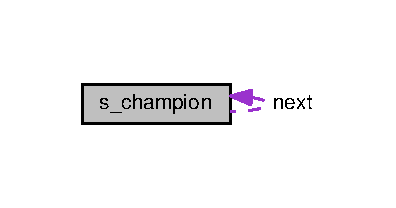
\includegraphics[width=190pt]{structs__champion__coll__graph}
\end{center}
\end{figure}
\subsection*{Data Fields}
\begin{DoxyCompactItemize}
\item 
\hypertarget{structs__champion_a28dc0293f716f3fbb2d0bd1cb83f93a2}{char {\bfseries name} \mbox{[}P\-R\-O\-G\-\_\-\-N\-A\-M\-E\-\_\-\-L\-E\-N\-G\-T\-H+1\mbox{]}}\label{structs__champion_a28dc0293f716f3fbb2d0bd1cb83f93a2}

\item 
\hypertarget{structs__champion_a439227feff9d7f55384e8780cfc2eb82}{int {\bfseries size}}\label{structs__champion_a439227feff9d7f55384e8780cfc2eb82}

\item 
\hypertarget{structs__champion_ae6da1ff2fd8abd8f79b0a42acf5b98b9}{char {\bfseries comment} \mbox{[}C\-O\-M\-M\-E\-N\-T\-\_\-\-L\-E\-N\-G\-T\-H+1\mbox{]}}\label{structs__champion_ae6da1ff2fd8abd8f79b0a42acf5b98b9}

\item 
\hypertarget{structs__champion_a7106e2abc437ad981830d14176d15f09}{int {\bfseries number}}\label{structs__champion_a7106e2abc437ad981830d14176d15f09}

\item 
\hypertarget{structs__champion_a45c6bc6d1135dc398bf8deae861a2ebc}{int {\bfseries address}}\label{structs__champion_a45c6bc6d1135dc398bf8deae861a2ebc}

\item 
\hypertarget{structs__champion_a10a8d8076a169aad66a5134a4b372c91}{unsigned char $\ast$ {\bfseries code}}\label{structs__champion_a10a8d8076a169aad66a5134a4b372c91}

\item 
\hypertarget{structs__champion_a2cb50263f0f7a37d88d397a1d0e66f3a}{int {\bfseries live}}\label{structs__champion_a2cb50263f0f7a37d88d397a1d0e66f3a}

\item 
\hypertarget{structs__champion_ac8c81e61335635fa4709d82412b31f06}{int {\bfseries pc}}\label{structs__champion_ac8c81e61335635fa4709d82412b31f06}

\item 
\hypertarget{structs__champion_a1853c17443a5893d3acd539b3c7a9289}{int {\bfseries wait\-\_\-time}}\label{structs__champion_a1853c17443a5893d3acd539b3c7a9289}

\item 
\hypertarget{structs__champion_a205e2cf1e11ba6a2f7110d4b650e971c}{int {\bfseries reg} \mbox{[}R\-E\-G\-\_\-\-N\-U\-M\-B\-E\-R+1\mbox{]}}\label{structs__champion_a205e2cf1e11ba6a2f7110d4b650e971c}

\item 
\hypertarget{structs__champion_ac33dd0ad72380ad7b52434992811c5a7}{int {\bfseries carry}}\label{structs__champion_ac33dd0ad72380ad7b52434992811c5a7}

\item 
\hypertarget{structs__champion_a2d18ffa3b1babc703aa8b1cd3812f7ad}{struct \hyperlink{structs__champion}{s\-\_\-champion} $\ast$ {\bfseries next}}\label{structs__champion_a2d18ffa3b1babc703aa8b1cd3812f7ad}

\end{DoxyCompactItemize}


\subsection{Detailed Description}


Definition at line 17 of file champion.\-h.



The documentation for this struct was generated from the following file\-:\begin{DoxyCompactItemize}
\item 
corewar/includes/champion.\-h\end{DoxyCompactItemize}

\hypertarget{structs__char}{\section{s\-\_\-char Struct Reference}
\label{structs__char}\index{s\-\_\-char@{s\-\_\-char}}
}


{\ttfamily \#include $<$get\-\_\-next\-\_\-line.\-h$>$}



Collaboration diagram for s\-\_\-char\-:\nopagebreak
\begin{figure}[H]
\begin{center}
\leavevmode
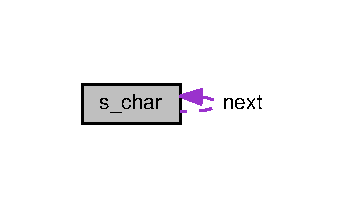
\includegraphics[width=166pt]{de/d73/structs__char__coll__graph}
\end{center}
\end{figure}
\subsection*{Data Fields}
\begin{DoxyCompactItemize}
\item 
char \hyperlink{structs__char_ac6027d2dbb9ac08b3b6729341c0bcf8f}{character}
\item 
struct \hyperlink{structs__char}{s\-\_\-char} $\ast$ \hyperlink{structs__char_a948ac1df44de106ac471ed05df56482c}{next}
\end{DoxyCompactItemize}


\subsection{Detailed Description}


Definition at line 16 of file get\-\_\-next\-\_\-line.\-h.



\subsection{Field Documentation}
\hypertarget{structs__char_ac6027d2dbb9ac08b3b6729341c0bcf8f}{\index{s\-\_\-char@{s\-\_\-char}!character@{character}}
\index{character@{character}!s_char@{s\-\_\-char}}
\subsubsection[{character}]{\setlength{\rightskip}{0pt plus 5cm}char character}}\label{structs__char_ac6027d2dbb9ac08b3b6729341c0bcf8f}


Definition at line 18 of file get\-\_\-next\-\_\-line.\-h.

\hypertarget{structs__char_a948ac1df44de106ac471ed05df56482c}{\index{s\-\_\-char@{s\-\_\-char}!next@{next}}
\index{next@{next}!s_char@{s\-\_\-char}}
\subsubsection[{next}]{\setlength{\rightskip}{0pt plus 5cm}struct {\bf s\-\_\-char}$\ast$ next}}\label{structs__char_a948ac1df44de106ac471ed05df56482c}


Definition at line 19 of file get\-\_\-next\-\_\-line.\-h.



The documentation for this struct was generated from the following file\-:\begin{DoxyCompactItemize}
\item 
lib/includes/\hyperlink{get__next__line_8h}{get\-\_\-next\-\_\-line.\-h}\end{DoxyCompactItemize}

\hypertarget{structs__corewar}{\section{s\-\_\-corewar Struct Reference}
\label{structs__corewar}\index{s\-\_\-corewar@{s\-\_\-corewar}}
}


Collaboration diagram for s\-\_\-corewar\-:
\nopagebreak
\begin{figure}[H]
\begin{center}
\leavevmode
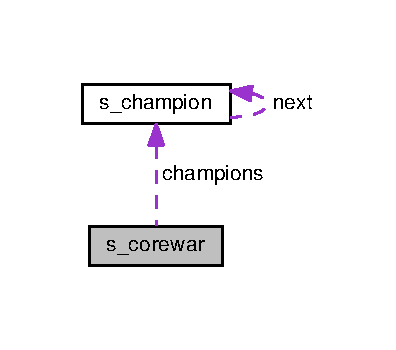
\includegraphics[width=190pt]{structs__corewar__coll__graph}
\end{center}
\end{figure}
\subsection*{Data Fields}
\begin{DoxyCompactItemize}
\item 
\hypertarget{structs__corewar_a28773f3c282d16757e3a3e1027825a17}{int {\bfseries dump}}\label{structs__corewar_a28773f3c282d16757e3a3e1027825a17}

\item 
\hypertarget{structs__corewar_a5a44dad6cc6d5d67cb34464b4f25e171}{unsigned int {\bfseries nbr\-\_\-champions}}\label{structs__corewar_a5a44dad6cc6d5d67cb34464b4f25e171}

\item 
\hypertarget{structs__corewar_a2d2d5697f388905b044f2cde1f481d2d}{\hyperlink{structs__champion}{t\-\_\-champion} $\ast$ {\bfseries champions}}\label{structs__corewar_a2d2d5697f388905b044f2cde1f481d2d}

\end{DoxyCompactItemize}


\subsection{Detailed Description}


Definition at line 16 of file corewar.\-h.



The documentation for this struct was generated from the following file\-:\begin{DoxyCompactItemize}
\item 
corewar/includes/corewar.\-h\end{DoxyCompactItemize}

\hypertarget{structs__glist}{\section{s\-\_\-glist Struct Reference}
\label{structs__glist}\index{s\-\_\-glist@{s\-\_\-glist}}
}


Collaboration diagram for s\-\_\-glist\-:
\nopagebreak
\begin{figure}[H]
\begin{center}
\leavevmode
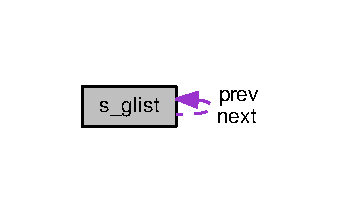
\includegraphics[width=165pt]{structs__glist__coll__graph}
\end{center}
\end{figure}
\subsection*{Data Fields}
\begin{DoxyCompactItemize}
\item 
\hypertarget{structs__glist_a735984d41155bc1032e09bece8f8d66d}{void $\ast$ {\bfseries data}}\label{structs__glist_a735984d41155bc1032e09bece8f8d66d}

\item 
\hypertarget{structs__glist_a20c22490f3a95677fd45a335958ea5da}{\hyperlink{structs__glist}{t\-\_\-glist} $\ast$ {\bfseries next}}\label{structs__glist_a20c22490f3a95677fd45a335958ea5da}

\item 
\hypertarget{structs__glist_a3d44f907f8e9a16abd22ce7aa098a912}{\hyperlink{structs__glist}{t\-\_\-glist} $\ast$ {\bfseries prev}}\label{structs__glist_a3d44f907f8e9a16abd22ce7aa098a912}

\end{DoxyCompactItemize}


\subsection{Detailed Description}


Definition at line 16 of file my\-\_\-malloc.\-h.



The documentation for this struct was generated from the following file\-:\begin{DoxyCompactItemize}
\item 
lib/includes/my\-\_\-malloc.\-h\end{DoxyCompactItemize}

\hypertarget{structs__latinfo}{\section{s\-\_\-latinfo Struct Reference}
\label{structs__latinfo}\index{s\-\_\-latinfo@{s\-\_\-latinfo}}
}


Collaboration diagram for s\-\_\-latinfo\-:
\nopagebreak
\begin{figure}[H]
\begin{center}
\leavevmode
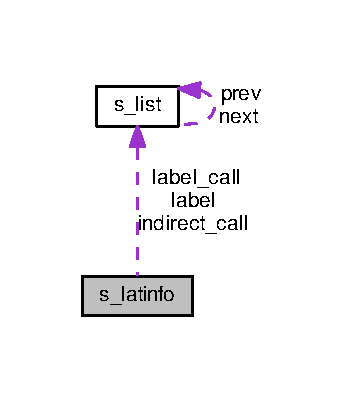
\includegraphics[width=166pt]{structs__latinfo__coll__graph}
\end{center}
\end{figure}
\subsection*{Data Fields}
\begin{DoxyCompactItemize}
\item 
\hypertarget{structs__latinfo_a565ba05926f2219e68cf55a13f15fbab}{int {\bfseries nbrinstruction}}\label{structs__latinfo_a565ba05926f2219e68cf55a13f15fbab}

\item 
\hypertarget{structs__latinfo_a53b5fc61b57ec971b013fa338a3adfc7}{\hyperlink{structs__list}{t\-\_\-list} $\ast$ {\bfseries label}}\label{structs__latinfo_a53b5fc61b57ec971b013fa338a3adfc7}

\item 
\hypertarget{structs__latinfo_ab7161df38e24c00cc4f576cec776ea81}{\hyperlink{structs__list}{t\-\_\-list} $\ast$ {\bfseries label\-\_\-call}}\label{structs__latinfo_ab7161df38e24c00cc4f576cec776ea81}

\item 
\hypertarget{structs__latinfo_a2644eca4f289d61e8f2e5923cf5a3a6c}{\hyperlink{structs__list}{t\-\_\-list} $\ast$ {\bfseries indirect\-\_\-call}}\label{structs__latinfo_a2644eca4f289d61e8f2e5923cf5a3a6c}

\end{DoxyCompactItemize}


\subsection{Detailed Description}


Definition at line 16 of file list\-\_\-lab\-\_\-in.\-h.



The documentation for this struct was generated from the following file\-:\begin{DoxyCompactItemize}
\item 
asm/includes/list\-\_\-lab\-\_\-in.\-h\end{DoxyCompactItemize}

\hypertarget{structs__list}{\section{s\-\_\-list Struct Reference}
\label{structs__list}\index{s\-\_\-list@{s\-\_\-list}}
}


{\ttfamily \#include $<$gen\-\_\-list.\-h$>$}



Collaboration diagram for s\-\_\-list\-:\nopagebreak
\begin{figure}[H]
\begin{center}
\leavevmode
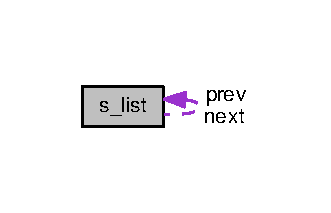
\includegraphics[width=159pt]{dd/d04/structs__list__coll__graph}
\end{center}
\end{figure}
\subsection*{Data Fields}
\begin{DoxyCompactItemize}
\item 
int \hyperlink{structs__list_a08f6b479f237e672809735f0764104e6}{num\-\_\-value\-\_\-a}
\item 
int \hyperlink{structs__list_a067e0fca9eda0eeac39cd8c6e7fe50c5}{num\-\_\-value\-\_\-b}
\item 
int \hyperlink{structs__list_a6709d69fcc8bb060ac025b812ac45550}{num\-\_\-value\-\_\-c}
\item 
char $\ast$ \hyperlink{structs__list_a50b6bdca20b777174be4fbdb217ca8d6}{str\-\_\-value}
\item 
\hyperlink{gen__list_8h_aefde00352c5326bb1c28ebd4404c4795}{t\-\_\-list} $\ast$ \hyperlink{structs__list_afb31ca295a227d12dae42eb9d7a61f40}{next}
\item 
\hyperlink{gen__list_8h_aefde00352c5326bb1c28ebd4404c4795}{t\-\_\-list} $\ast$ \hyperlink{structs__list_a58d5321b61e8202cbad3ede333207719}{prev}
\end{DoxyCompactItemize}


\subsection{Detailed Description}


Definition at line 16 of file gen\-\_\-list.\-h.



\subsection{Field Documentation}
\hypertarget{structs__list_afb31ca295a227d12dae42eb9d7a61f40}{\index{s\-\_\-list@{s\-\_\-list}!next@{next}}
\index{next@{next}!s_list@{s\-\_\-list}}
\subsubsection[{next}]{\setlength{\rightskip}{0pt plus 5cm}{\bf t\-\_\-list}$\ast$ next}}\label{structs__list_afb31ca295a227d12dae42eb9d7a61f40}


Definition at line 22 of file gen\-\_\-list.\-h.

\hypertarget{structs__list_a08f6b479f237e672809735f0764104e6}{\index{s\-\_\-list@{s\-\_\-list}!num\-\_\-value\-\_\-a@{num\-\_\-value\-\_\-a}}
\index{num\-\_\-value\-\_\-a@{num\-\_\-value\-\_\-a}!s_list@{s\-\_\-list}}
\subsubsection[{num\-\_\-value\-\_\-a}]{\setlength{\rightskip}{0pt plus 5cm}int num\-\_\-value\-\_\-a}}\label{structs__list_a08f6b479f237e672809735f0764104e6}


Definition at line 18 of file gen\-\_\-list.\-h.

\hypertarget{structs__list_a067e0fca9eda0eeac39cd8c6e7fe50c5}{\index{s\-\_\-list@{s\-\_\-list}!num\-\_\-value\-\_\-b@{num\-\_\-value\-\_\-b}}
\index{num\-\_\-value\-\_\-b@{num\-\_\-value\-\_\-b}!s_list@{s\-\_\-list}}
\subsubsection[{num\-\_\-value\-\_\-b}]{\setlength{\rightskip}{0pt plus 5cm}int num\-\_\-value\-\_\-b}}\label{structs__list_a067e0fca9eda0eeac39cd8c6e7fe50c5}


Definition at line 19 of file gen\-\_\-list.\-h.

\hypertarget{structs__list_a6709d69fcc8bb060ac025b812ac45550}{\index{s\-\_\-list@{s\-\_\-list}!num\-\_\-value\-\_\-c@{num\-\_\-value\-\_\-c}}
\index{num\-\_\-value\-\_\-c@{num\-\_\-value\-\_\-c}!s_list@{s\-\_\-list}}
\subsubsection[{num\-\_\-value\-\_\-c}]{\setlength{\rightskip}{0pt plus 5cm}int num\-\_\-value\-\_\-c}}\label{structs__list_a6709d69fcc8bb060ac025b812ac45550}


Definition at line 20 of file gen\-\_\-list.\-h.

\hypertarget{structs__list_a58d5321b61e8202cbad3ede333207719}{\index{s\-\_\-list@{s\-\_\-list}!prev@{prev}}
\index{prev@{prev}!s_list@{s\-\_\-list}}
\subsubsection[{prev}]{\setlength{\rightskip}{0pt plus 5cm}{\bf t\-\_\-list}$\ast$ prev}}\label{structs__list_a58d5321b61e8202cbad3ede333207719}


Definition at line 23 of file gen\-\_\-list.\-h.

\hypertarget{structs__list_a50b6bdca20b777174be4fbdb217ca8d6}{\index{s\-\_\-list@{s\-\_\-list}!str\-\_\-value@{str\-\_\-value}}
\index{str\-\_\-value@{str\-\_\-value}!s_list@{s\-\_\-list}}
\subsubsection[{str\-\_\-value}]{\setlength{\rightskip}{0pt plus 5cm}char$\ast$ str\-\_\-value}}\label{structs__list_a50b6bdca20b777174be4fbdb217ca8d6}


Definition at line 21 of file gen\-\_\-list.\-h.



The documentation for this struct was generated from the following file\-:\begin{DoxyCompactItemize}
\item 
lib/includes/\hyperlink{gen__list_8h}{gen\-\_\-list.\-h}\end{DoxyCompactItemize}

\hypertarget{structs__pos__info}{\section{s\-\_\-pos\-\_\-info Struct Reference}
\label{structs__pos__info}\index{s\-\_\-pos\-\_\-info@{s\-\_\-pos\-\_\-info}}
}


{\ttfamily \#include $<$compile.\-h$>$}

\subsection*{Data Fields}
\begin{DoxyCompactItemize}
\item 
int \hyperlink{structs__pos__info_a3d2291cda4e654eefa396b1bc08e0a67}{whereiam}
\item 
int \hyperlink{structs__pos__info_a6a372b8459e7ab7a3f7dadc86300eeca}{to\-\_\-cur\-\_\-in}
\end{DoxyCompactItemize}


\subsection{Detailed Description}


Definition at line 21 of file compile.\-h.



\subsection{Field Documentation}
\hypertarget{structs__pos__info_a6a372b8459e7ab7a3f7dadc86300eeca}{\index{s\-\_\-pos\-\_\-info@{s\-\_\-pos\-\_\-info}!to\-\_\-cur\-\_\-in@{to\-\_\-cur\-\_\-in}}
\index{to\-\_\-cur\-\_\-in@{to\-\_\-cur\-\_\-in}!s_pos_info@{s\-\_\-pos\-\_\-info}}
\subsubsection[{to\-\_\-cur\-\_\-in}]{\setlength{\rightskip}{0pt plus 5cm}int to\-\_\-cur\-\_\-in}}\label{structs__pos__info_a6a372b8459e7ab7a3f7dadc86300eeca}


Definition at line 24 of file compile.\-h.

\hypertarget{structs__pos__info_a3d2291cda4e654eefa396b1bc08e0a67}{\index{s\-\_\-pos\-\_\-info@{s\-\_\-pos\-\_\-info}!whereiam@{whereiam}}
\index{whereiam@{whereiam}!s_pos_info@{s\-\_\-pos\-\_\-info}}
\subsubsection[{whereiam}]{\setlength{\rightskip}{0pt plus 5cm}int whereiam}}\label{structs__pos__info_a3d2291cda4e654eefa396b1bc08e0a67}


Definition at line 23 of file compile.\-h.



The documentation for this struct was generated from the following file\-:\begin{DoxyCompactItemize}
\item 
asm/includes/\hyperlink{compile_8h}{compile.\-h}\end{DoxyCompactItemize}

\hypertarget{unionu__int}{\section{u\-\_\-int Union Reference}
\label{unionu__int}\index{u\-\_\-int@{u\-\_\-int}}
}


{\ttfamily \#include $<$corewar.\-h$>$}

\subsection*{Data Fields}
\begin{DoxyCompactItemize}
\item 
int \hyperlink{unionu__int_acb559820d9ca11295b4500f179ef6392}{i}
\item 
char \hyperlink{unionu__int_a4430fee26e106ac5b7a95a966e1de8fb}{c} \mbox{[}4\mbox{]}
\end{DoxyCompactItemize}


\subsection{Detailed Description}


Definition at line 23 of file corewar.\-h.



\subsection{Field Documentation}
\hypertarget{unionu__int_a4430fee26e106ac5b7a95a966e1de8fb}{\index{u\-\_\-int@{u\-\_\-int}!c@{c}}
\index{c@{c}!u_int@{u\-\_\-int}}
\subsubsection[{c}]{\setlength{\rightskip}{0pt plus 5cm}char c\mbox{[}4\mbox{]}}}\label{unionu__int_a4430fee26e106ac5b7a95a966e1de8fb}


Definition at line 26 of file corewar.\-h.

\hypertarget{unionu__int_acb559820d9ca11295b4500f179ef6392}{\index{u\-\_\-int@{u\-\_\-int}!i@{i}}
\index{i@{i}!u_int@{u\-\_\-int}}
\subsubsection[{i}]{\setlength{\rightskip}{0pt plus 5cm}int i}}\label{unionu__int_acb559820d9ca11295b4500f179ef6392}


Definition at line 25 of file corewar.\-h.



The documentation for this union was generated from the following file\-:\begin{DoxyCompactItemize}
\item 
corewar/includes/\hyperlink{corewar_8h}{corewar.\-h}\end{DoxyCompactItemize}

\hypertarget{unionu__int__rev}{\section{u\-\_\-int\-\_\-rev Union Reference}
\label{unionu__int__rev}\index{u\-\_\-int\-\_\-rev@{u\-\_\-int\-\_\-rev}}
}


{\ttfamily \#include $<$corewar.\-h$>$}

\subsection*{Data Fields}
\begin{DoxyCompactItemize}
\item 
char \hyperlink{unionu__int__rev_a4430fee26e106ac5b7a95a966e1de8fb}{c} \mbox{[}4\mbox{]}
\item 
int \hyperlink{unionu__int__rev_acb559820d9ca11295b4500f179ef6392}{i}
\end{DoxyCompactItemize}


\subsection{Detailed Description}


Definition at line 16 of file corewar.\-h.



\subsection{Field Documentation}
\hypertarget{unionu__int__rev_a4430fee26e106ac5b7a95a966e1de8fb}{\index{u\-\_\-int\-\_\-rev@{u\-\_\-int\-\_\-rev}!c@{c}}
\index{c@{c}!u_int_rev@{u\-\_\-int\-\_\-rev}}
\subsubsection[{c}]{\setlength{\rightskip}{0pt plus 5cm}char c\mbox{[}4\mbox{]}}}\label{unionu__int__rev_a4430fee26e106ac5b7a95a966e1de8fb}


Definition at line 18 of file corewar.\-h.

\hypertarget{unionu__int__rev_acb559820d9ca11295b4500f179ef6392}{\index{u\-\_\-int\-\_\-rev@{u\-\_\-int\-\_\-rev}!i@{i}}
\index{i@{i}!u_int_rev@{u\-\_\-int\-\_\-rev}}
\subsubsection[{i}]{\setlength{\rightskip}{0pt plus 5cm}int i}}\label{unionu__int__rev_acb559820d9ca11295b4500f179ef6392}


Definition at line 19 of file corewar.\-h.



The documentation for this union was generated from the following file\-:\begin{DoxyCompactItemize}
\item 
corewar/includes/\hyperlink{corewar_8h}{corewar.\-h}\end{DoxyCompactItemize}

\chapter{File Documentation}
\hypertarget{check_8h}{\section{asm/includes/check.h File Reference}
\label{check_8h}\index{asm/includes/check.\-h@{asm/includes/check.\-h}}
}
This graph shows which files directly or indirectly include this file\-:\nopagebreak
\begin{figure}[H]
\begin{center}
\leavevmode
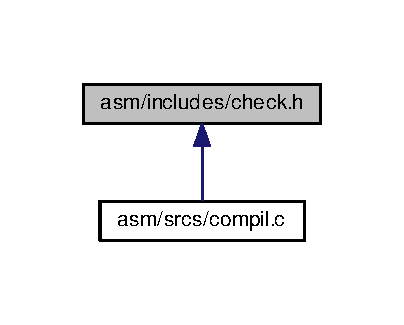
\includegraphics[width=194pt]{d8/dae/check_8h__dep__incl}
\end{center}
\end{figure}
\subsection*{Functions}
\begin{DoxyCompactItemize}
\item 
int \hyperlink{check_8h_a3733c5d12a474ef3f52f2b842588a5e9}{my\-\_\-check\-\_\-param} (\hyperlink{op_8h_a4819392a6eb5f0799ea856ae99557fba}{args\-\_\-type\-\_\-t} type, char $\ast$param)
\item 
int \hyperlink{check_8h_aca2977c58b7518e22098bd8bd5a5f313}{my\-\_\-check\-\_\-params} (int i, \hyperlink{op_8h_a51ce7549e6b9948b233d73c4c0d0fe02}{op\-\_\-t} $\ast$optodo, char $\ast$$\ast$lexed\-\_\-line)
\end{DoxyCompactItemize}


\subsection{Function Documentation}
\hypertarget{check_8h_a3733c5d12a474ef3f52f2b842588a5e9}{\index{check.\-h@{check.\-h}!my\-\_\-check\-\_\-param@{my\-\_\-check\-\_\-param}}
\index{my\-\_\-check\-\_\-param@{my\-\_\-check\-\_\-param}!check.h@{check.\-h}}
\subsubsection[{my\-\_\-check\-\_\-param}]{\setlength{\rightskip}{0pt plus 5cm}int my\-\_\-check\-\_\-param (
\begin{DoxyParamCaption}
\item[{{\bf args\-\_\-type\-\_\-t}}]{type, }
\item[{char $\ast$}]{param}
\end{DoxyParamCaption}
)}}\label{check_8h_a3733c5d12a474ef3f52f2b842588a5e9}


Definition at line 21 of file check\-\_\-param.\-c.



Here is the call graph for this function\-:\nopagebreak
\begin{figure}[H]
\begin{center}
\leavevmode
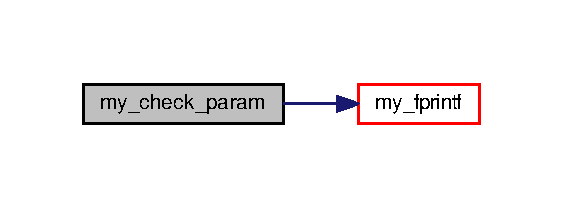
\includegraphics[width=270pt]{d6/d38/check_8h_a3733c5d12a474ef3f52f2b842588a5e9_cgraph}
\end{center}
\end{figure}




Here is the caller graph for this function\-:\nopagebreak
\begin{figure}[H]
\begin{center}
\leavevmode
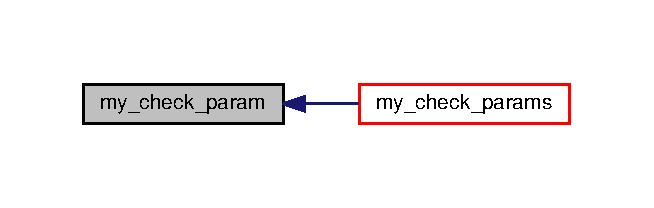
\includegraphics[width=314pt]{d6/d38/check_8h_a3733c5d12a474ef3f52f2b842588a5e9_icgraph}
\end{center}
\end{figure}


\hypertarget{check_8h_aca2977c58b7518e22098bd8bd5a5f313}{\index{check.\-h@{check.\-h}!my\-\_\-check\-\_\-params@{my\-\_\-check\-\_\-params}}
\index{my\-\_\-check\-\_\-params@{my\-\_\-check\-\_\-params}!check.h@{check.\-h}}
\subsubsection[{my\-\_\-check\-\_\-params}]{\setlength{\rightskip}{0pt plus 5cm}int my\-\_\-check\-\_\-params (
\begin{DoxyParamCaption}
\item[{int}]{i, }
\item[{{\bf op\-\_\-t} $\ast$}]{optodo, }
\item[{char $\ast$$\ast$}]{lexed\-\_\-line}
\end{DoxyParamCaption}
)}}\label{check_8h_aca2977c58b7518e22098bd8bd5a5f313}


Definition at line 48 of file check\-\_\-param.\-c.



Here is the call graph for this function\-:\nopagebreak
\begin{figure}[H]
\begin{center}
\leavevmode
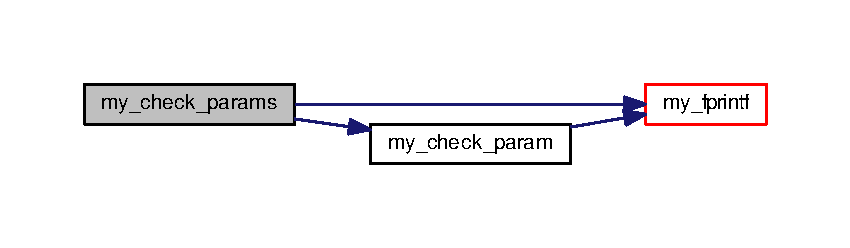
\includegraphics[width=350pt]{d6/d38/check_8h_aca2977c58b7518e22098bd8bd5a5f313_cgraph}
\end{center}
\end{figure}




Here is the caller graph for this function\-:\nopagebreak
\begin{figure}[H]
\begin{center}
\leavevmode
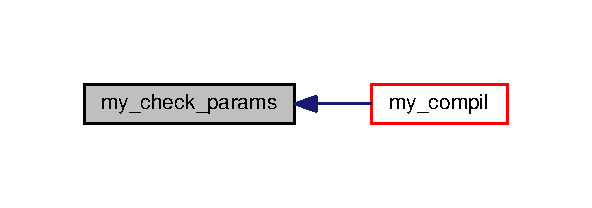
\includegraphics[width=284pt]{d6/d38/check_8h_aca2977c58b7518e22098bd8bd5a5f313_icgraph}
\end{center}
\end{figure}



\hypertarget{compile_8h}{\section{asm/includes/compile.h File Reference}
\label{compile_8h}\index{asm/includes/compile.\-h@{asm/includes/compile.\-h}}
}
{\ttfamily \#include \char`\"{}list\-\_\-lab\-\_\-in.\-h\char`\"{}}\\*
{\ttfamily \#include \char`\"{}op.\-h\char`\"{}}\\*
Include dependency graph for compile.\-h\-:
\nopagebreak
\begin{figure}[H]
\begin{center}
\leavevmode
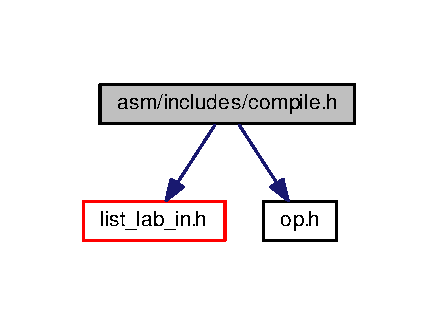
\includegraphics[width=210pt]{d9/d70/compile_8h__incl}
\end{center}
\end{figure}
This graph shows which files directly or indirectly include this file\-:
\nopagebreak
\begin{figure}[H]
\begin{center}
\leavevmode
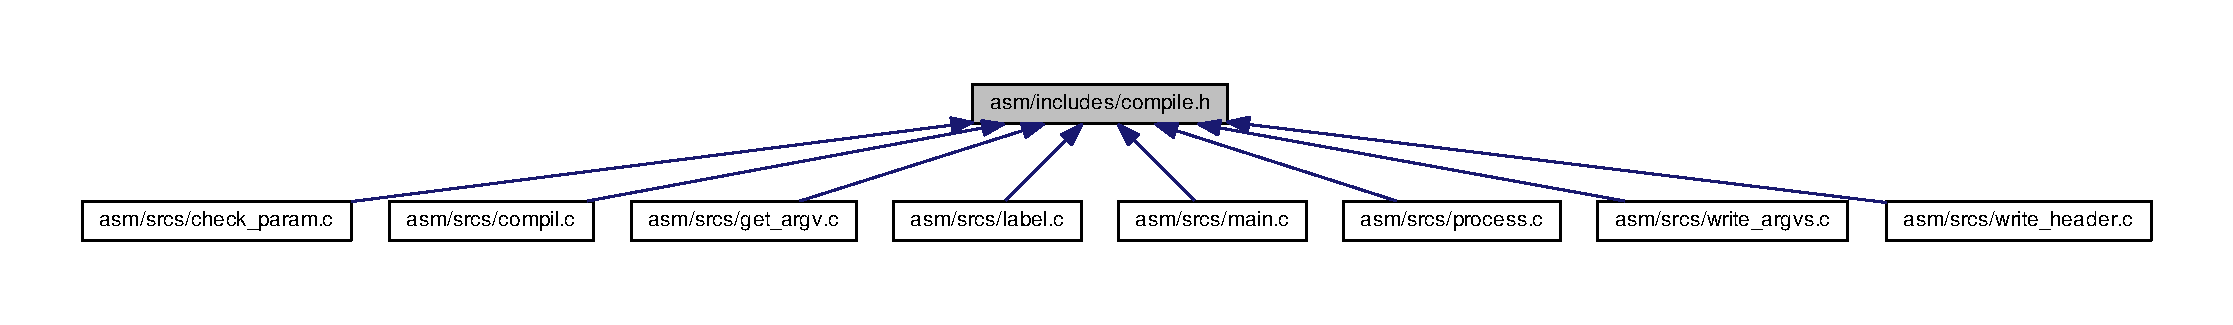
\includegraphics[width=350pt]{d3/d75/compile_8h__dep__incl}
\end{center}
\end{figure}
\subsection*{Data Structures}
\begin{DoxyCompactItemize}
\item 
struct \hyperlink{structs__pos__info}{s\-\_\-pos\-\_\-info}
\end{DoxyCompactItemize}
\subsection*{Macros}
\begin{DoxyCompactItemize}
\item 
\#define \hyperlink{compile_8h_a49999be01380f41cc0d0f1f1406fb277}{H\-E\-A\-D\-E\-R\-\_\-\-S\-I\-Z\-E}~(8 + \hyperlink{op_8h_a2bd1b5655c5d92af5ebe7f4bb3436b73}{P\-R\-O\-G\-\_\-\-N\-A\-M\-E\-\_\-\-L\-E\-N\-G\-T\-H} + \hyperlink{op_8h_a31a10f5d8e8f9085ce0224cf043cb5fa}{C\-O\-M\-M\-E\-N\-T\-\_\-\-L\-E\-N\-G\-T\-H})
\item 
\#define \hyperlink{compile_8h_a5cb439d9f933fde4cf23caa370c030e7}{W\-A\-R\-N\-I\-N\-G}~\char`\"{}\textbackslash{}33\mbox{[}33;1m\-Warning \-:\textbackslash{}33\mbox{[}0m\char`\"{}
\item 
\#define \hyperlink{compile_8h_a8fe83ac76edc595f6b98cd4a4127aed5}{E\-R\-R\-O\-R}~\char`\"{}\textbackslash{}33\mbox{[}31;1m\-Error \-:\textbackslash{}33\mbox{[}0m\char`\"{}
\item 
\#define \hyperlink{compile_8h_a1ad73526ce07d2f3564dfd83c982ca3f}{N\-O\-T\-E}~\char`\"{}\textbackslash{}33\mbox{[}32;1m\-Note \-:\textbackslash{}33\mbox{[}0m\char`\"{}
\end{DoxyCompactItemize}
\subsection*{Typedefs}
\begin{DoxyCompactItemize}
\item 
typedef struct \hyperlink{structs__pos__info}{s\-\_\-pos\-\_\-info} \hyperlink{compile_8h_a55d668897c420e8b402208277c8fc669}{t\-\_\-pos\-\_\-info}
\end{DoxyCompactItemize}
\subsection*{Functions}
\begin{DoxyCompactItemize}
\item 
\hyperlink{compile_8h_a55d668897c420e8b402208277c8fc669}{t\-\_\-pos\-\_\-info} \hyperlink{compile_8h_ab8d8242eec2c52dd2b194c3df9db1bb9}{my\-\_\-fuse} (int pos, int instruc)
\item 
int \hyperlink{compile_8h_ac90570dbce495f89534c76073a2c1831}{my\-\_\-compil} (char $\ast$$\ast$lexed\-\_\-line, \hyperlink{op_8h_a51ce7549e6b9948b233d73c4c0d0fe02}{op\-\_\-t} $\ast$optodo, int fd\-\_\-binary)
\item 
int \hyperlink{compile_8h_ae9aa8d794f6c75aa3c6b131a15fcb7ca}{my\-\_\-parsefile} (int fd\-\_\-champ, int fd\-\_\-binary)
\item 
char $\ast$ \hyperlink{compile_8h_aa932b29ee343cca4dc71dc5922c8e899}{get\-\_\-quotes} (const char $\ast$str)
\item 
int \hyperlink{compile_8h_a07317474f4f23ef25856daa71b8534da}{header\-\_\-size\-\_\-prog} (int fd\-\_\-bin, int writed)
\item 
int \hyperlink{compile_8h_af66636c0f888f33983f6630fa1911bae}{late\-\_\-operation} (int fd\-\_\-bin, int writed, \hyperlink{list__lab__in_8h_a91fca2551b14cd3e3c189afabae27a0b}{t\-\_\-lateinfo} $\ast$info)
\item 
int \hyperlink{compile_8h_a1ad3c381180e678695983d1c91157f3c}{check\-\_\-if\-\_\-valid\-\_\-label} (char $\ast$str)
\item 
int \hyperlink{compile_8h_a68e75f6dc19bf1ad207e4ede39a78a91}{get\-\_\-label\-\_\-def} (\hyperlink{list__lab__in_8h_a91fca2551b14cd3e3c189afabae27a0b}{t\-\_\-lateinfo} $\ast$info, char $\ast$$\ast$lexed\-\_\-line, int fileoffset)
\item 
int \hyperlink{compile_8h_ace181743a8765de7c256cfd2ceb042a6}{get\-\_\-lateparam} (\hyperlink{list__lab__in_8h_a91fca2551b14cd3e3c189afabae27a0b}{t\-\_\-lateinfo} $\ast$info, char $\ast$$\ast$lexed\-\_\-line, int fileoffset, \hyperlink{op_8h_a51ce7549e6b9948b233d73c4c0d0fe02}{op\-\_\-t} $\ast$optodo)
\item 
char $\ast$ \hyperlink{compile_8h_ac304120f3bbaed766d710046bdfe0e2e}{put\-\_\-in\-\_\-char} (int nbr, int size)
\end{DoxyCompactItemize}


\subsection{Macro Definition Documentation}
\hypertarget{compile_8h_a8fe83ac76edc595f6b98cd4a4127aed5}{\index{compile.\-h@{compile.\-h}!E\-R\-R\-O\-R@{E\-R\-R\-O\-R}}
\index{E\-R\-R\-O\-R@{E\-R\-R\-O\-R}!compile.h@{compile.\-h}}
\subsubsection[{E\-R\-R\-O\-R}]{\setlength{\rightskip}{0pt plus 5cm}\#define E\-R\-R\-O\-R~\char`\"{}\textbackslash{}33\mbox{[}31;1m\-Error \-:\textbackslash{}33\mbox{[}0m\char`\"{}}}\label{compile_8h_a8fe83ac76edc595f6b98cd4a4127aed5}


Definition at line 18 of file compile.\-h.

\hypertarget{compile_8h_a49999be01380f41cc0d0f1f1406fb277}{\index{compile.\-h@{compile.\-h}!H\-E\-A\-D\-E\-R\-\_\-\-S\-I\-Z\-E@{H\-E\-A\-D\-E\-R\-\_\-\-S\-I\-Z\-E}}
\index{H\-E\-A\-D\-E\-R\-\_\-\-S\-I\-Z\-E@{H\-E\-A\-D\-E\-R\-\_\-\-S\-I\-Z\-E}!compile.h@{compile.\-h}}
\subsubsection[{H\-E\-A\-D\-E\-R\-\_\-\-S\-I\-Z\-E}]{\setlength{\rightskip}{0pt plus 5cm}\#define H\-E\-A\-D\-E\-R\-\_\-\-S\-I\-Z\-E~(8 + {\bf P\-R\-O\-G\-\_\-\-N\-A\-M\-E\-\_\-\-L\-E\-N\-G\-T\-H} + {\bf C\-O\-M\-M\-E\-N\-T\-\_\-\-L\-E\-N\-G\-T\-H})}}\label{compile_8h_a49999be01380f41cc0d0f1f1406fb277}


Definition at line 16 of file compile.\-h.

\hypertarget{compile_8h_a1ad73526ce07d2f3564dfd83c982ca3f}{\index{compile.\-h@{compile.\-h}!N\-O\-T\-E@{N\-O\-T\-E}}
\index{N\-O\-T\-E@{N\-O\-T\-E}!compile.h@{compile.\-h}}
\subsubsection[{N\-O\-T\-E}]{\setlength{\rightskip}{0pt plus 5cm}\#define N\-O\-T\-E~\char`\"{}\textbackslash{}33\mbox{[}32;1m\-Note \-:\textbackslash{}33\mbox{[}0m\char`\"{}}}\label{compile_8h_a1ad73526ce07d2f3564dfd83c982ca3f}


Definition at line 19 of file compile.\-h.

\hypertarget{compile_8h_a5cb439d9f933fde4cf23caa370c030e7}{\index{compile.\-h@{compile.\-h}!W\-A\-R\-N\-I\-N\-G@{W\-A\-R\-N\-I\-N\-G}}
\index{W\-A\-R\-N\-I\-N\-G@{W\-A\-R\-N\-I\-N\-G}!compile.h@{compile.\-h}}
\subsubsection[{W\-A\-R\-N\-I\-N\-G}]{\setlength{\rightskip}{0pt plus 5cm}\#define W\-A\-R\-N\-I\-N\-G~\char`\"{}\textbackslash{}33\mbox{[}33;1m\-Warning \-:\textbackslash{}33\mbox{[}0m\char`\"{}}}\label{compile_8h_a5cb439d9f933fde4cf23caa370c030e7}


Definition at line 17 of file compile.\-h.



\subsection{Typedef Documentation}
\hypertarget{compile_8h_a55d668897c420e8b402208277c8fc669}{\index{compile.\-h@{compile.\-h}!t\-\_\-pos\-\_\-info@{t\-\_\-pos\-\_\-info}}
\index{t\-\_\-pos\-\_\-info@{t\-\_\-pos\-\_\-info}!compile.h@{compile.\-h}}
\subsubsection[{t\-\_\-pos\-\_\-info}]{\setlength{\rightskip}{0pt plus 5cm}typedef struct {\bf s\-\_\-pos\-\_\-info}		 {\bf t\-\_\-pos\-\_\-info}}}\label{compile_8h_a55d668897c420e8b402208277c8fc669}


\subsection{Function Documentation}
\hypertarget{compile_8h_a1ad3c381180e678695983d1c91157f3c}{\index{compile.\-h@{compile.\-h}!check\-\_\-if\-\_\-valid\-\_\-label@{check\-\_\-if\-\_\-valid\-\_\-label}}
\index{check\-\_\-if\-\_\-valid\-\_\-label@{check\-\_\-if\-\_\-valid\-\_\-label}!compile.h@{compile.\-h}}
\subsubsection[{check\-\_\-if\-\_\-valid\-\_\-label}]{\setlength{\rightskip}{0pt plus 5cm}int check\-\_\-if\-\_\-valid\-\_\-label (
\begin{DoxyParamCaption}
\item[{char $\ast$}]{str}
\end{DoxyParamCaption}
)}}\label{compile_8h_a1ad3c381180e678695983d1c91157f3c}


Definition at line 74 of file check\-\_\-param.\-c.



Here is the call graph for this function\-:\nopagebreak
\begin{figure}[H]
\begin{center}
\leavevmode
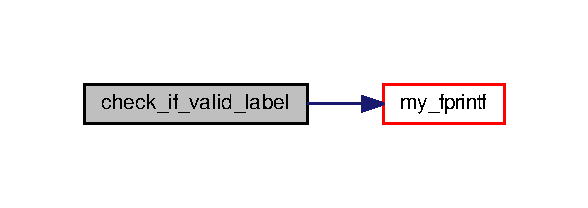
\includegraphics[width=282pt]{d4/d03/compile_8h_a1ad3c381180e678695983d1c91157f3c_cgraph}
\end{center}
\end{figure}




Here is the caller graph for this function\-:\nopagebreak
\begin{figure}[H]
\begin{center}
\leavevmode
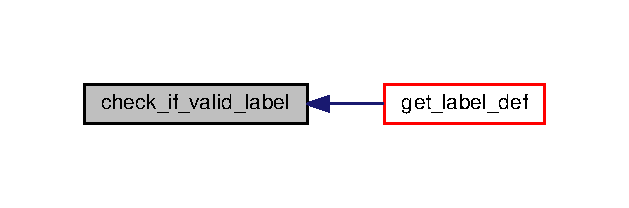
\includegraphics[width=302pt]{d4/d03/compile_8h_a1ad3c381180e678695983d1c91157f3c_icgraph}
\end{center}
\end{figure}


\hypertarget{compile_8h_a68e75f6dc19bf1ad207e4ede39a78a91}{\index{compile.\-h@{compile.\-h}!get\-\_\-label\-\_\-def@{get\-\_\-label\-\_\-def}}
\index{get\-\_\-label\-\_\-def@{get\-\_\-label\-\_\-def}!compile.h@{compile.\-h}}
\subsubsection[{get\-\_\-label\-\_\-def}]{\setlength{\rightskip}{0pt plus 5cm}int get\-\_\-label\-\_\-def (
\begin{DoxyParamCaption}
\item[{{\bf t\-\_\-lateinfo} $\ast$}]{info, }
\item[{char $\ast$$\ast$}]{lexed\-\_\-line, }
\item[{int}]{fileoffset}
\end{DoxyParamCaption}
)}}\label{compile_8h_a68e75f6dc19bf1ad207e4ede39a78a91}


Definition at line 84 of file label.\-c.



Here is the call graph for this function\-:\nopagebreak
\begin{figure}[H]
\begin{center}
\leavevmode
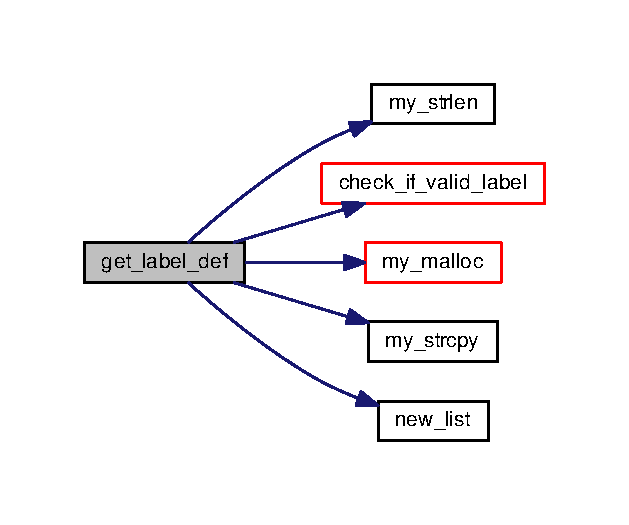
\includegraphics[width=302pt]{d4/d03/compile_8h_a68e75f6dc19bf1ad207e4ede39a78a91_cgraph}
\end{center}
\end{figure}




Here is the caller graph for this function\-:\nopagebreak
\begin{figure}[H]
\begin{center}
\leavevmode
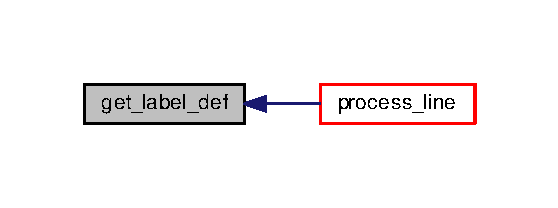
\includegraphics[width=268pt]{d4/d03/compile_8h_a68e75f6dc19bf1ad207e4ede39a78a91_icgraph}
\end{center}
\end{figure}


\hypertarget{compile_8h_ace181743a8765de7c256cfd2ceb042a6}{\index{compile.\-h@{compile.\-h}!get\-\_\-lateparam@{get\-\_\-lateparam}}
\index{get\-\_\-lateparam@{get\-\_\-lateparam}!compile.h@{compile.\-h}}
\subsubsection[{get\-\_\-lateparam}]{\setlength{\rightskip}{0pt plus 5cm}int get\-\_\-lateparam (
\begin{DoxyParamCaption}
\item[{{\bf t\-\_\-lateinfo} $\ast$}]{info, }
\item[{char $\ast$$\ast$}]{lexed\-\_\-line, }
\item[{int}]{fileoffset, }
\item[{{\bf op\-\_\-t} $\ast$}]{optodo}
\end{DoxyParamCaption}
)}}\label{compile_8h_ace181743a8765de7c256cfd2ceb042a6}


Definition at line 143 of file label.\-c.



Here is the call graph for this function\-:\nopagebreak
\begin{figure}[H]
\begin{center}
\leavevmode
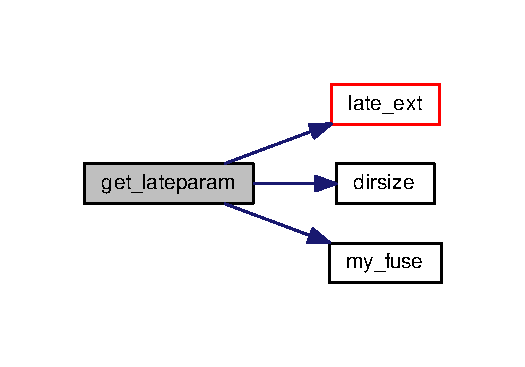
\includegraphics[width=252pt]{d4/d03/compile_8h_ace181743a8765de7c256cfd2ceb042a6_cgraph}
\end{center}
\end{figure}




Here is the caller graph for this function\-:\nopagebreak
\begin{figure}[H]
\begin{center}
\leavevmode
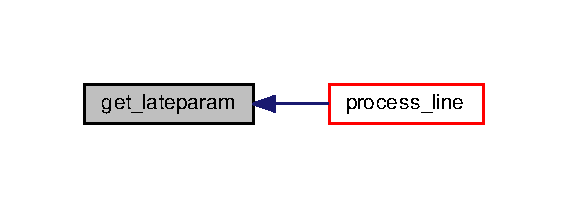
\includegraphics[width=272pt]{d4/d03/compile_8h_ace181743a8765de7c256cfd2ceb042a6_icgraph}
\end{center}
\end{figure}


\hypertarget{compile_8h_aa932b29ee343cca4dc71dc5922c8e899}{\index{compile.\-h@{compile.\-h}!get\-\_\-quotes@{get\-\_\-quotes}}
\index{get\-\_\-quotes@{get\-\_\-quotes}!compile.h@{compile.\-h}}
\subsubsection[{get\-\_\-quotes}]{\setlength{\rightskip}{0pt plus 5cm}char$\ast$ get\-\_\-quotes (
\begin{DoxyParamCaption}
\item[{const char $\ast$}]{str}
\end{DoxyParamCaption}
)}}\label{compile_8h_aa932b29ee343cca4dc71dc5922c8e899}
\hypertarget{compile_8h_a07317474f4f23ef25856daa71b8534da}{\index{compile.\-h@{compile.\-h}!header\-\_\-size\-\_\-prog@{header\-\_\-size\-\_\-prog}}
\index{header\-\_\-size\-\_\-prog@{header\-\_\-size\-\_\-prog}!compile.h@{compile.\-h}}
\subsubsection[{header\-\_\-size\-\_\-prog}]{\setlength{\rightskip}{0pt plus 5cm}int header\-\_\-size\-\_\-prog (
\begin{DoxyParamCaption}
\item[{int}]{fd\-\_\-bin, }
\item[{int}]{writed}
\end{DoxyParamCaption}
)}}\label{compile_8h_a07317474f4f23ef25856daa71b8534da}


Definition at line 31 of file label.\-c.



Here is the call graph for this function\-:\nopagebreak
\begin{figure}[H]
\begin{center}
\leavevmode
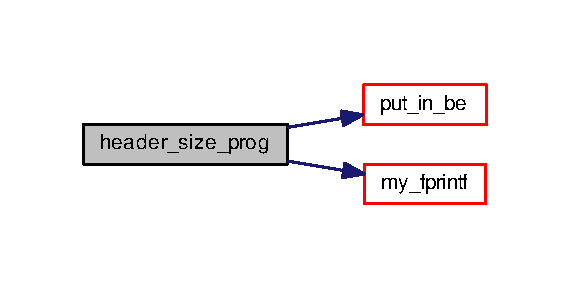
\includegraphics[width=274pt]{d4/d03/compile_8h_a07317474f4f23ef25856daa71b8534da_cgraph}
\end{center}
\end{figure}




Here is the caller graph for this function\-:\nopagebreak
\begin{figure}[H]
\begin{center}
\leavevmode
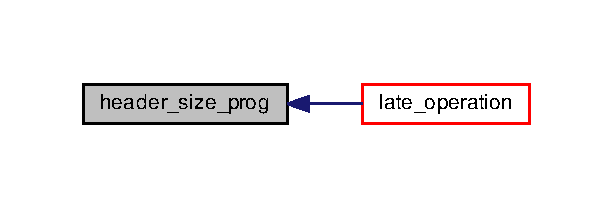
\includegraphics[width=294pt]{d4/d03/compile_8h_a07317474f4f23ef25856daa71b8534da_icgraph}
\end{center}
\end{figure}


\hypertarget{compile_8h_af66636c0f888f33983f6630fa1911bae}{\index{compile.\-h@{compile.\-h}!late\-\_\-operation@{late\-\_\-operation}}
\index{late\-\_\-operation@{late\-\_\-operation}!compile.h@{compile.\-h}}
\subsubsection[{late\-\_\-operation}]{\setlength{\rightskip}{0pt plus 5cm}int late\-\_\-operation (
\begin{DoxyParamCaption}
\item[{int}]{fd\-\_\-bin, }
\item[{int}]{writed, }
\item[{{\bf t\-\_\-lateinfo} $\ast$}]{info}
\end{DoxyParamCaption}
)}}\label{compile_8h_af66636c0f888f33983f6630fa1911bae}


Definition at line 50 of file label.\-c.



Here is the call graph for this function\-:\nopagebreak
\begin{figure}[H]
\begin{center}
\leavevmode
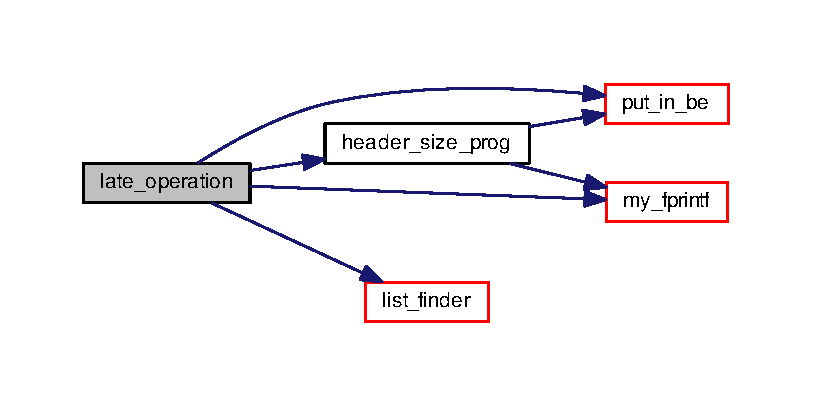
\includegraphics[width=350pt]{d4/d03/compile_8h_af66636c0f888f33983f6630fa1911bae_cgraph}
\end{center}
\end{figure}




Here is the caller graph for this function\-:\nopagebreak
\begin{figure}[H]
\begin{center}
\leavevmode
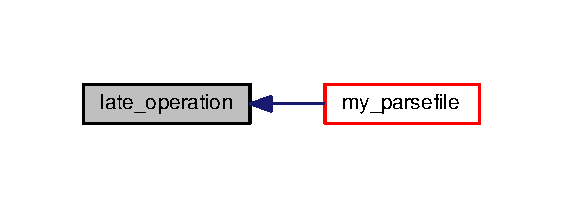
\includegraphics[width=270pt]{d4/d03/compile_8h_af66636c0f888f33983f6630fa1911bae_icgraph}
\end{center}
\end{figure}


\hypertarget{compile_8h_ac90570dbce495f89534c76073a2c1831}{\index{compile.\-h@{compile.\-h}!my\-\_\-compil@{my\-\_\-compil}}
\index{my\-\_\-compil@{my\-\_\-compil}!compile.h@{compile.\-h}}
\subsubsection[{my\-\_\-compil}]{\setlength{\rightskip}{0pt plus 5cm}int my\-\_\-compil (
\begin{DoxyParamCaption}
\item[{char $\ast$$\ast$}]{lexed\-\_\-line, }
\item[{{\bf op\-\_\-t} $\ast$}]{optodo, }
\item[{int}]{fd\-\_\-binary}
\end{DoxyParamCaption}
)}}\label{compile_8h_ac90570dbce495f89534c76073a2c1831}


Definition at line 33 of file compil.\-c.



Here is the call graph for this function\-:\nopagebreak
\begin{figure}[H]
\begin{center}
\leavevmode
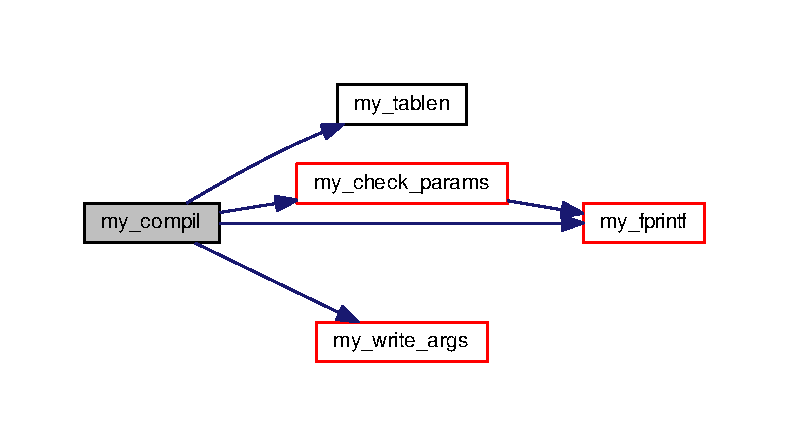
\includegraphics[width=350pt]{d4/d03/compile_8h_ac90570dbce495f89534c76073a2c1831_cgraph}
\end{center}
\end{figure}




Here is the caller graph for this function\-:\nopagebreak
\begin{figure}[H]
\begin{center}
\leavevmode
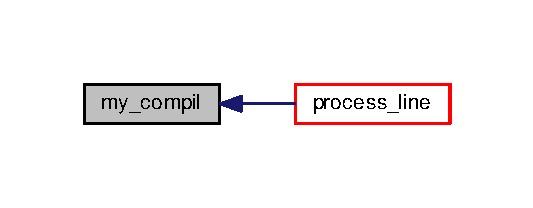
\includegraphics[width=256pt]{d4/d03/compile_8h_ac90570dbce495f89534c76073a2c1831_icgraph}
\end{center}
\end{figure}


\hypertarget{compile_8h_ab8d8242eec2c52dd2b194c3df9db1bb9}{\index{compile.\-h@{compile.\-h}!my\-\_\-fuse@{my\-\_\-fuse}}
\index{my\-\_\-fuse@{my\-\_\-fuse}!compile.h@{compile.\-h}}
\subsubsection[{my\-\_\-fuse}]{\setlength{\rightskip}{0pt plus 5cm}{\bf t\-\_\-pos\-\_\-info} my\-\_\-fuse (
\begin{DoxyParamCaption}
\item[{int}]{pos, }
\item[{int}]{instruc}
\end{DoxyParamCaption}
)}}\label{compile_8h_ab8d8242eec2c52dd2b194c3df9db1bb9}


Definition at line 114 of file process.\-c.



Here is the caller graph for this function\-:\nopagebreak
\begin{figure}[H]
\begin{center}
\leavevmode
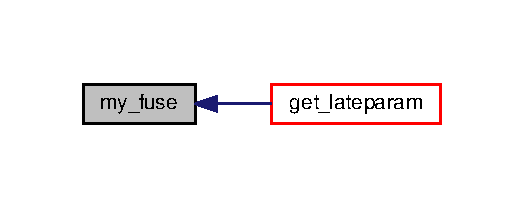
\includegraphics[width=252pt]{d4/d03/compile_8h_ab8d8242eec2c52dd2b194c3df9db1bb9_icgraph}
\end{center}
\end{figure}


\hypertarget{compile_8h_ae9aa8d794f6c75aa3c6b131a15fcb7ca}{\index{compile.\-h@{compile.\-h}!my\-\_\-parsefile@{my\-\_\-parsefile}}
\index{my\-\_\-parsefile@{my\-\_\-parsefile}!compile.h@{compile.\-h}}
\subsubsection[{my\-\_\-parsefile}]{\setlength{\rightskip}{0pt plus 5cm}int my\-\_\-parsefile (
\begin{DoxyParamCaption}
\item[{int}]{fd\-\_\-champ, }
\item[{int}]{fd\-\_\-binary}
\end{DoxyParamCaption}
)}}\label{compile_8h_ae9aa8d794f6c75aa3c6b131a15fcb7ca}


Definition at line 113 of file compil.\-c.



Here is the call graph for this function\-:
\nopagebreak
\begin{figure}[H]
\begin{center}
\leavevmode
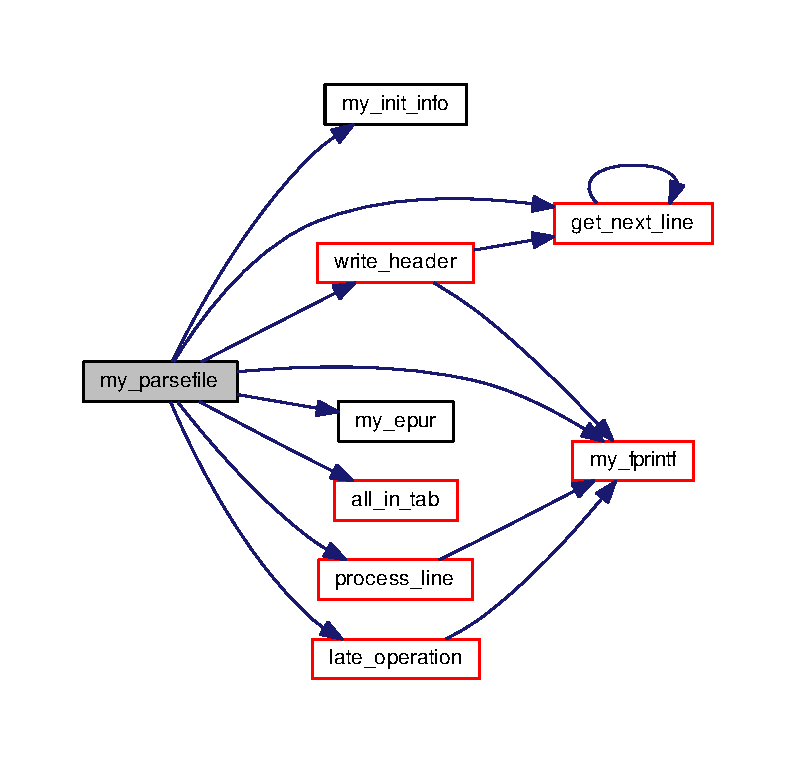
\includegraphics[width=350pt]{d4/d03/compile_8h_ae9aa8d794f6c75aa3c6b131a15fcb7ca_cgraph}
\end{center}
\end{figure}




Here is the caller graph for this function\-:\nopagebreak
\begin{figure}[H]
\begin{center}
\leavevmode
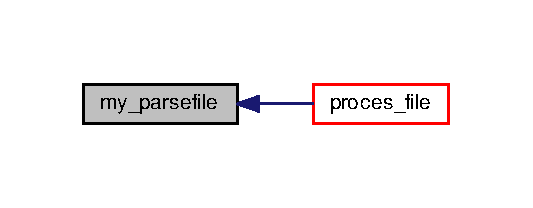
\includegraphics[width=256pt]{d4/d03/compile_8h_ae9aa8d794f6c75aa3c6b131a15fcb7ca_icgraph}
\end{center}
\end{figure}


\hypertarget{compile_8h_ac304120f3bbaed766d710046bdfe0e2e}{\index{compile.\-h@{compile.\-h}!put\-\_\-in\-\_\-char@{put\-\_\-in\-\_\-char}}
\index{put\-\_\-in\-\_\-char@{put\-\_\-in\-\_\-char}!compile.h@{compile.\-h}}
\subsubsection[{put\-\_\-in\-\_\-char}]{\setlength{\rightskip}{0pt plus 5cm}char$\ast$ put\-\_\-in\-\_\-char (
\begin{DoxyParamCaption}
\item[{int}]{nbr, }
\item[{int}]{size}
\end{DoxyParamCaption}
)}}\label{compile_8h_ac304120f3bbaed766d710046bdfe0e2e}

\hypertarget{get__argv_8h}{\section{asm/includes/get\-\_\-argv.h File Reference}
\label{get__argv_8h}\index{asm/includes/get\-\_\-argv.\-h@{asm/includes/get\-\_\-argv.\-h}}
}
This graph shows which files directly or indirectly include this file\-:\nopagebreak
\begin{figure}[H]
\begin{center}
\leavevmode
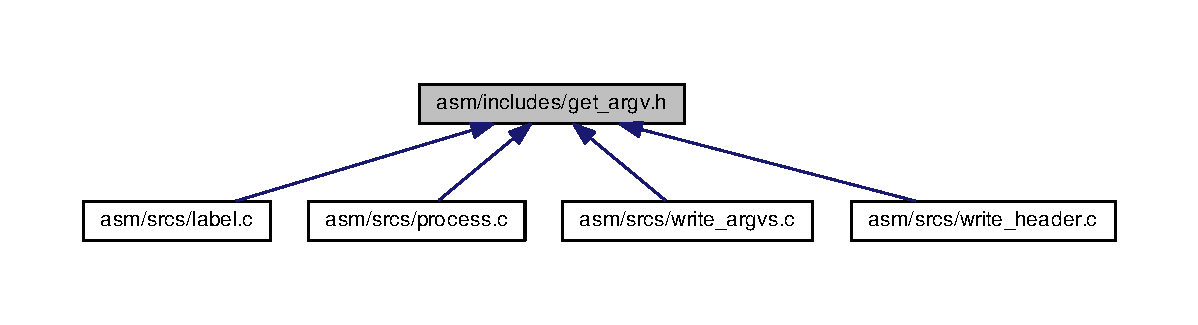
\includegraphics[width=350pt]{d9/d1d/get__argv_8h__dep__incl}
\end{center}
\end{figure}
\subsection*{Functions}
\begin{DoxyCompactItemize}
\item 
char $\ast$ \hyperlink{get__argv_8h_a0b2ae2ba08582e01f1fa3a02a42e4014}{get\-\_\-fname} (char $\ast$fname, char $\ast$str)
\item 
char $\ast$ \hyperlink{get__argv_8h_a4e291b57bd0c553d7bbad7f3e5b7cd50}{get\-\_\-quotes\-\_\-name} (const char $\ast$str, char ret\mbox{[}$\,$\mbox{]})
\item 
char $\ast$ \hyperlink{get__argv_8h_a91d9889f105aba2ceba52a0554c4d872}{get\-\_\-quotes\-\_\-comment} (const char $\ast$str, char ret\mbox{[}$\,$\mbox{]})
\end{DoxyCompactItemize}


\subsection{Function Documentation}
\hypertarget{get__argv_8h_a0b2ae2ba08582e01f1fa3a02a42e4014}{\index{get\-\_\-argv.\-h@{get\-\_\-argv.\-h}!get\-\_\-fname@{get\-\_\-fname}}
\index{get\-\_\-fname@{get\-\_\-fname}!get_argv.h@{get\-\_\-argv.\-h}}
\subsubsection[{get\-\_\-fname}]{\setlength{\rightskip}{0pt plus 5cm}char$\ast$ get\-\_\-fname (
\begin{DoxyParamCaption}
\item[{char $\ast$}]{fname, }
\item[{char $\ast$}]{str}
\end{DoxyParamCaption}
)}}\label{get__argv_8h_a0b2ae2ba08582e01f1fa3a02a42e4014}


Definition at line 24 of file get\-\_\-argv.\-c.



Here is the call graph for this function\-:\nopagebreak
\begin{figure}[H]
\begin{center}
\leavevmode
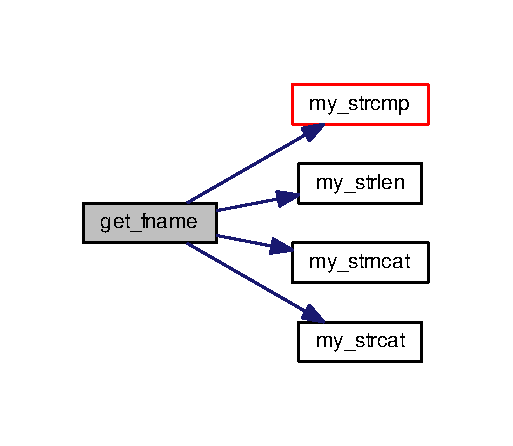
\includegraphics[width=246pt]{df/db6/get__argv_8h_a0b2ae2ba08582e01f1fa3a02a42e4014_cgraph}
\end{center}
\end{figure}




Here is the caller graph for this function\-:\nopagebreak
\begin{figure}[H]
\begin{center}
\leavevmode
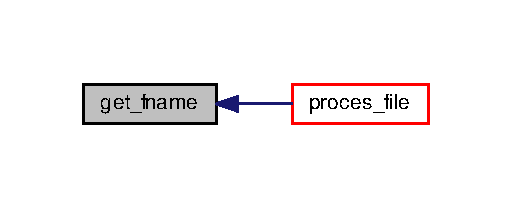
\includegraphics[width=246pt]{df/db6/get__argv_8h_a0b2ae2ba08582e01f1fa3a02a42e4014_icgraph}
\end{center}
\end{figure}


\hypertarget{get__argv_8h_a91d9889f105aba2ceba52a0554c4d872}{\index{get\-\_\-argv.\-h@{get\-\_\-argv.\-h}!get\-\_\-quotes\-\_\-comment@{get\-\_\-quotes\-\_\-comment}}
\index{get\-\_\-quotes\-\_\-comment@{get\-\_\-quotes\-\_\-comment}!get_argv.h@{get\-\_\-argv.\-h}}
\subsubsection[{get\-\_\-quotes\-\_\-comment}]{\setlength{\rightskip}{0pt plus 5cm}char$\ast$ get\-\_\-quotes\-\_\-comment (
\begin{DoxyParamCaption}
\item[{const char $\ast$}]{str, }
\item[{char}]{ret\mbox{[}$\,$\mbox{]}}
\end{DoxyParamCaption}
)}}\label{get__argv_8h_a91d9889f105aba2ceba52a0554c4d872}


Definition at line 45 of file get\-\_\-argv.\-c.



Here is the call graph for this function\-:\nopagebreak
\begin{figure}[H]
\begin{center}
\leavevmode
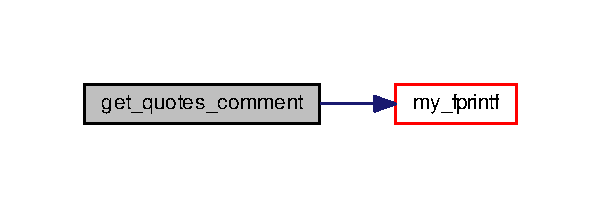
\includegraphics[width=288pt]{df/db6/get__argv_8h_a91d9889f105aba2ceba52a0554c4d872_cgraph}
\end{center}
\end{figure}




Here is the caller graph for this function\-:\nopagebreak
\begin{figure}[H]
\begin{center}
\leavevmode
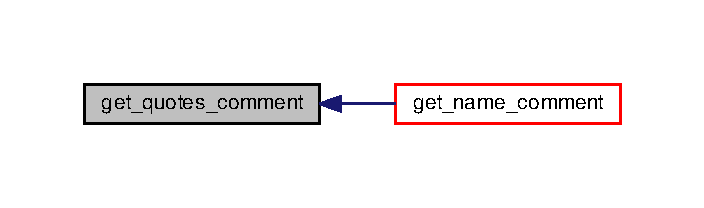
\includegraphics[width=338pt]{df/db6/get__argv_8h_a91d9889f105aba2ceba52a0554c4d872_icgraph}
\end{center}
\end{figure}


\hypertarget{get__argv_8h_a4e291b57bd0c553d7bbad7f3e5b7cd50}{\index{get\-\_\-argv.\-h@{get\-\_\-argv.\-h}!get\-\_\-quotes\-\_\-name@{get\-\_\-quotes\-\_\-name}}
\index{get\-\_\-quotes\-\_\-name@{get\-\_\-quotes\-\_\-name}!get_argv.h@{get\-\_\-argv.\-h}}
\subsubsection[{get\-\_\-quotes\-\_\-name}]{\setlength{\rightskip}{0pt plus 5cm}char$\ast$ get\-\_\-quotes\-\_\-name (
\begin{DoxyParamCaption}
\item[{const char $\ast$}]{str, }
\item[{char}]{ret\mbox{[}$\,$\mbox{]}}
\end{DoxyParamCaption}
)}}\label{get__argv_8h_a4e291b57bd0c553d7bbad7f3e5b7cd50}


Definition at line 79 of file get\-\_\-argv.\-c.



Here is the call graph for this function\-:\nopagebreak
\begin{figure}[H]
\begin{center}
\leavevmode
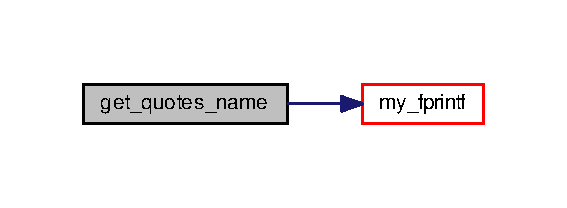
\includegraphics[width=272pt]{df/db6/get__argv_8h_a4e291b57bd0c553d7bbad7f3e5b7cd50_cgraph}
\end{center}
\end{figure}




Here is the caller graph for this function\-:\nopagebreak
\begin{figure}[H]
\begin{center}
\leavevmode
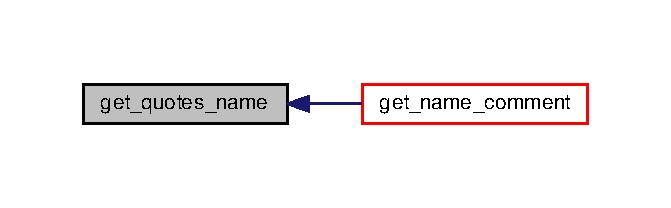
\includegraphics[width=322pt]{df/db6/get__argv_8h_a4e291b57bd0c553d7bbad7f3e5b7cd50_icgraph}
\end{center}
\end{figure}



\hypertarget{lexer_8h}{\section{asm/includes/lexer.h File Reference}
\label{lexer_8h}\index{asm/includes/lexer.\-h@{asm/includes/lexer.\-h}}
}
This graph shows which files directly or indirectly include this file\-:\nopagebreak
\begin{figure}[H]
\begin{center}
\leavevmode
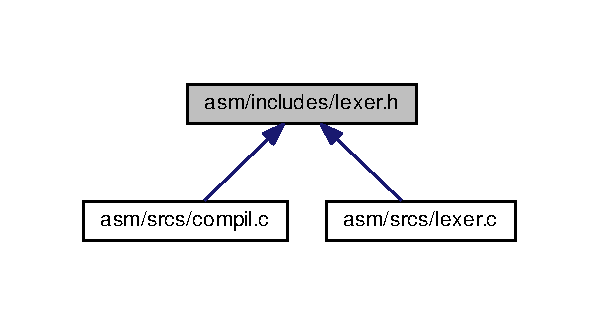
\includegraphics[width=287pt]{dc/d58/lexer_8h__dep__incl}
\end{center}
\end{figure}
\subsection*{Macros}
\begin{DoxyCompactItemize}
\item 
\#define \hyperlink{lexer_8h_aef8ab998cdd9d9dde4bf02dc8a2e00dd}{S\-E\-P\-A\-R\-A\-T\-O\-R\-\_\-\-C\-H\-A\-R2}~' '
\end{DoxyCompactItemize}
\subsection*{Functions}
\begin{DoxyCompactItemize}
\item 
int \hyperlink{lexer_8h_a5b06789e7faa2a3d6702a45ea299d028}{my\-\_\-add\-\_\-all} (int $\ast$i, char $\ast$str, int $\ast$j, char $\ast$$\ast$tabl)
\item 
void \hyperlink{lexer_8h_ab6ee845de2d75fa50b3afbc3112cc98d}{my\-\_\-add\-\_\-param} (char $\ast$str, int $\ast$j, char $\ast$$\ast$tabl, int i)
\item 
char $\ast$$\ast$ \hyperlink{lexer_8h_a9d987a70c88ab33366a6178db448c456}{all\-\_\-in\-\_\-tab\-\_\-base} (char $\ast$str, int word)
\item 
char $\ast$$\ast$ \hyperlink{lexer_8h_a5ebef41d60c4e6b6aa88bd8fd44e8422}{all\-\_\-in\-\_\-tab} (char $\ast$str)
\item 
void \hyperlink{lexer_8h_ae07e4d968ee702cb282f6d1235fdecff}{remove\-\_\-str\-\_\-in\-\_\-tab} (char $\ast$$\ast$tab, int x)
\end{DoxyCompactItemize}


\subsection{Macro Definition Documentation}
\hypertarget{lexer_8h_aef8ab998cdd9d9dde4bf02dc8a2e00dd}{\index{lexer.\-h@{lexer.\-h}!S\-E\-P\-A\-R\-A\-T\-O\-R\-\_\-\-C\-H\-A\-R2@{S\-E\-P\-A\-R\-A\-T\-O\-R\-\_\-\-C\-H\-A\-R2}}
\index{S\-E\-P\-A\-R\-A\-T\-O\-R\-\_\-\-C\-H\-A\-R2@{S\-E\-P\-A\-R\-A\-T\-O\-R\-\_\-\-C\-H\-A\-R2}!lexer.h@{lexer.\-h}}
\subsubsection[{S\-E\-P\-A\-R\-A\-T\-O\-R\-\_\-\-C\-H\-A\-R2}]{\setlength{\rightskip}{0pt plus 5cm}\#define S\-E\-P\-A\-R\-A\-T\-O\-R\-\_\-\-C\-H\-A\-R2~' '}}\label{lexer_8h_aef8ab998cdd9d9dde4bf02dc8a2e00dd}


Definition at line 14 of file lexer.\-h.



\subsection{Function Documentation}
\hypertarget{lexer_8h_a5ebef41d60c4e6b6aa88bd8fd44e8422}{\index{lexer.\-h@{lexer.\-h}!all\-\_\-in\-\_\-tab@{all\-\_\-in\-\_\-tab}}
\index{all\-\_\-in\-\_\-tab@{all\-\_\-in\-\_\-tab}!lexer.h@{lexer.\-h}}
\subsubsection[{all\-\_\-in\-\_\-tab}]{\setlength{\rightskip}{0pt plus 5cm}char$\ast$$\ast$ all\-\_\-in\-\_\-tab (
\begin{DoxyParamCaption}
\item[{char $\ast$}]{str}
\end{DoxyParamCaption}
)}}\label{lexer_8h_a5ebef41d60c4e6b6aa88bd8fd44e8422}


Definition at line 105 of file lexer.\-c.



Here is the call graph for this function\-:\nopagebreak
\begin{figure}[H]
\begin{center}
\leavevmode
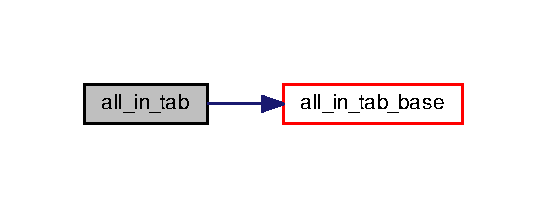
\includegraphics[width=262pt]{d5/df3/lexer_8h_a5ebef41d60c4e6b6aa88bd8fd44e8422_cgraph}
\end{center}
\end{figure}




Here is the caller graph for this function\-:\nopagebreak
\begin{figure}[H]
\begin{center}
\leavevmode
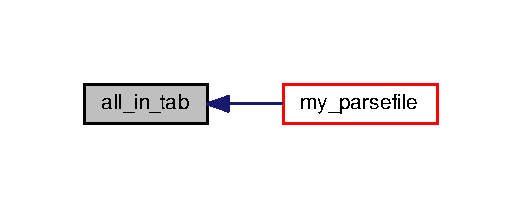
\includegraphics[width=250pt]{d5/df3/lexer_8h_a5ebef41d60c4e6b6aa88bd8fd44e8422_icgraph}
\end{center}
\end{figure}


\hypertarget{lexer_8h_a9d987a70c88ab33366a6178db448c456}{\index{lexer.\-h@{lexer.\-h}!all\-\_\-in\-\_\-tab\-\_\-base@{all\-\_\-in\-\_\-tab\-\_\-base}}
\index{all\-\_\-in\-\_\-tab\-\_\-base@{all\-\_\-in\-\_\-tab\-\_\-base}!lexer.h@{lexer.\-h}}
\subsubsection[{all\-\_\-in\-\_\-tab\-\_\-base}]{\setlength{\rightskip}{0pt plus 5cm}char$\ast$$\ast$ all\-\_\-in\-\_\-tab\-\_\-base (
\begin{DoxyParamCaption}
\item[{char $\ast$}]{str, }
\item[{int}]{word}
\end{DoxyParamCaption}
)}}\label{lexer_8h_a9d987a70c88ab33366a6178db448c456}


Definition at line 78 of file lexer.\-c.



Here is the call graph for this function\-:\nopagebreak
\begin{figure}[H]
\begin{center}
\leavevmode
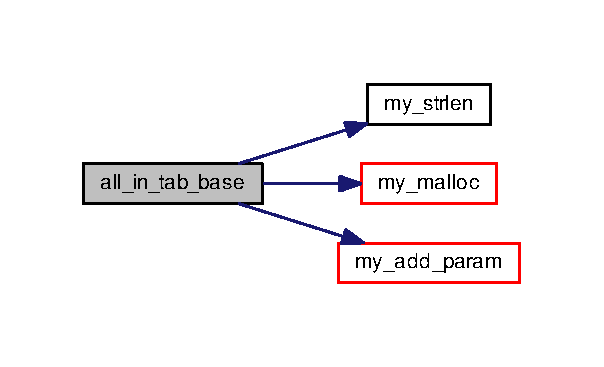
\includegraphics[width=290pt]{d5/df3/lexer_8h_a9d987a70c88ab33366a6178db448c456_cgraph}
\end{center}
\end{figure}




Here is the caller graph for this function\-:\nopagebreak
\begin{figure}[H]
\begin{center}
\leavevmode
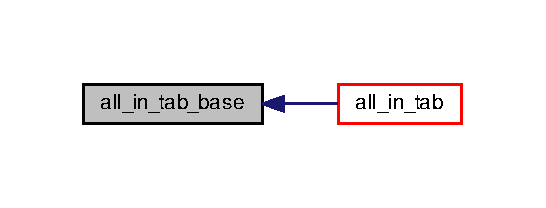
\includegraphics[width=262pt]{d5/df3/lexer_8h_a9d987a70c88ab33366a6178db448c456_icgraph}
\end{center}
\end{figure}


\hypertarget{lexer_8h_a5b06789e7faa2a3d6702a45ea299d028}{\index{lexer.\-h@{lexer.\-h}!my\-\_\-add\-\_\-all@{my\-\_\-add\-\_\-all}}
\index{my\-\_\-add\-\_\-all@{my\-\_\-add\-\_\-all}!lexer.h@{lexer.\-h}}
\subsubsection[{my\-\_\-add\-\_\-all}]{\setlength{\rightskip}{0pt plus 5cm}int my\-\_\-add\-\_\-all (
\begin{DoxyParamCaption}
\item[{int $\ast$}]{i, }
\item[{char $\ast$}]{str, }
\item[{int $\ast$}]{j, }
\item[{char $\ast$$\ast$}]{tabl}
\end{DoxyParamCaption}
)}}\label{lexer_8h_a5b06789e7faa2a3d6702a45ea299d028}


Definition at line 17 of file lexer.\-c.



Here is the call graph for this function\-:\nopagebreak
\begin{figure}[H]
\begin{center}
\leavevmode
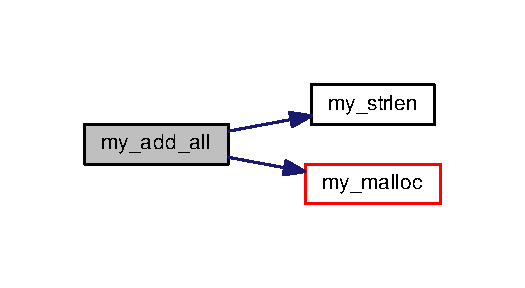
\includegraphics[width=252pt]{d5/df3/lexer_8h_a5b06789e7faa2a3d6702a45ea299d028_cgraph}
\end{center}
\end{figure}


\hypertarget{lexer_8h_ab6ee845de2d75fa50b3afbc3112cc98d}{\index{lexer.\-h@{lexer.\-h}!my\-\_\-add\-\_\-param@{my\-\_\-add\-\_\-param}}
\index{my\-\_\-add\-\_\-param@{my\-\_\-add\-\_\-param}!lexer.h@{lexer.\-h}}
\subsubsection[{my\-\_\-add\-\_\-param}]{\setlength{\rightskip}{0pt plus 5cm}void my\-\_\-add\-\_\-param (
\begin{DoxyParamCaption}
\item[{char $\ast$}]{str, }
\item[{int $\ast$}]{j, }
\item[{char $\ast$$\ast$}]{tabl, }
\item[{int}]{i}
\end{DoxyParamCaption}
)}}\label{lexer_8h_ab6ee845de2d75fa50b3afbc3112cc98d}


Definition at line 49 of file lexer.\-c.



Here is the call graph for this function\-:\nopagebreak
\begin{figure}[H]
\begin{center}
\leavevmode
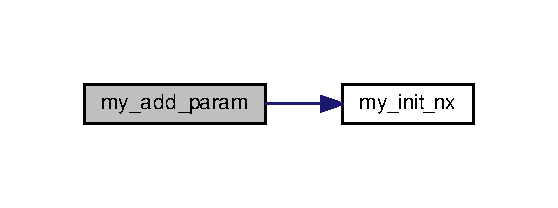
\includegraphics[width=268pt]{d5/df3/lexer_8h_ab6ee845de2d75fa50b3afbc3112cc98d_cgraph}
\end{center}
\end{figure}




Here is the caller graph for this function\-:\nopagebreak
\begin{figure}[H]
\begin{center}
\leavevmode
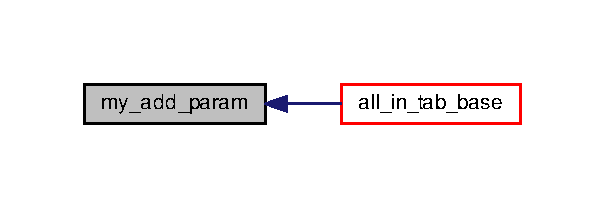
\includegraphics[width=290pt]{d5/df3/lexer_8h_ab6ee845de2d75fa50b3afbc3112cc98d_icgraph}
\end{center}
\end{figure}


\hypertarget{lexer_8h_ae07e4d968ee702cb282f6d1235fdecff}{\index{lexer.\-h@{lexer.\-h}!remove\-\_\-str\-\_\-in\-\_\-tab@{remove\-\_\-str\-\_\-in\-\_\-tab}}
\index{remove\-\_\-str\-\_\-in\-\_\-tab@{remove\-\_\-str\-\_\-in\-\_\-tab}!lexer.h@{lexer.\-h}}
\subsubsection[{remove\-\_\-str\-\_\-in\-\_\-tab}]{\setlength{\rightskip}{0pt plus 5cm}void remove\-\_\-str\-\_\-in\-\_\-tab (
\begin{DoxyParamCaption}
\item[{char $\ast$$\ast$}]{tab, }
\item[{int}]{x}
\end{DoxyParamCaption}
)}}\label{lexer_8h_ae07e4d968ee702cb282f6d1235fdecff}

\hypertarget{list__lab__in_8h}{\section{asm/includes/list\-\_\-lab\-\_\-in.h File Reference}
\label{list__lab__in_8h}\index{asm/includes/list\-\_\-lab\-\_\-in.\-h@{asm/includes/list\-\_\-lab\-\_\-in.\-h}}
}
{\ttfamily \#include \char`\"{}gen\-\_\-list.\-h\char`\"{}}\\*
Include dependency graph for list\-\_\-lab\-\_\-in.\-h\-:\nopagebreak
\begin{figure}[H]
\begin{center}
\leavevmode
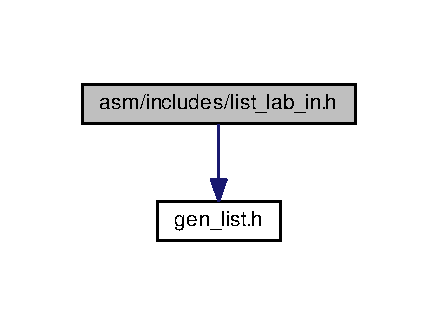
\includegraphics[width=210pt]{d3/dd0/list__lab__in_8h__incl}
\end{center}
\end{figure}
This graph shows which files directly or indirectly include this file\-:\nopagebreak
\begin{figure}[H]
\begin{center}
\leavevmode
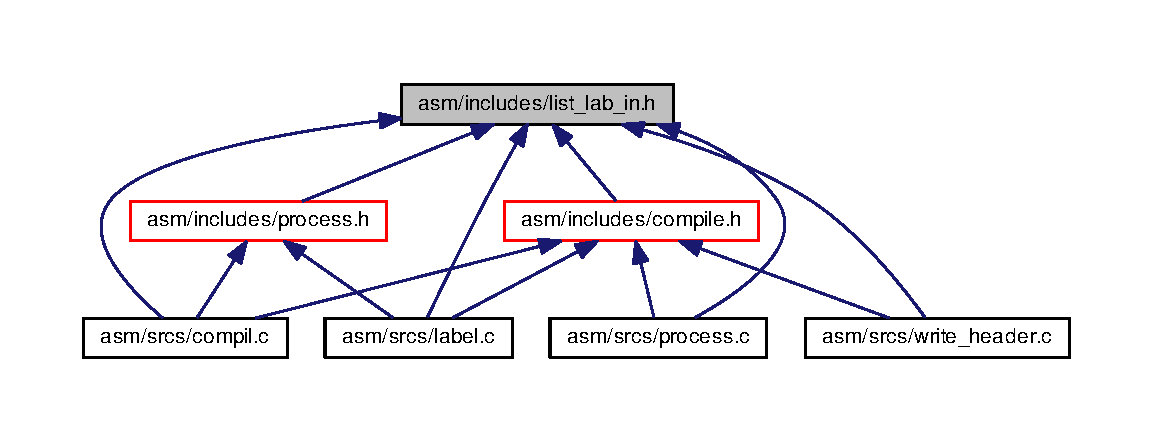
\includegraphics[width=350pt]{d5/dd0/list__lab__in_8h__dep__incl}
\end{center}
\end{figure}
\subsection*{Data Structures}
\begin{DoxyCompactItemize}
\item 
struct \hyperlink{structs__latinfo}{s\-\_\-latinfo}
\end{DoxyCompactItemize}
\subsection*{Typedefs}
\begin{DoxyCompactItemize}
\item 
typedef struct \hyperlink{structs__latinfo}{s\-\_\-latinfo} \hyperlink{list__lab__in_8h_a91fca2551b14cd3e3c189afabae27a0b}{t\-\_\-lateinfo}
\end{DoxyCompactItemize}


\subsection{Typedef Documentation}
\hypertarget{list__lab__in_8h_a91fca2551b14cd3e3c189afabae27a0b}{\index{list\-\_\-lab\-\_\-in.\-h@{list\-\_\-lab\-\_\-in.\-h}!t\-\_\-lateinfo@{t\-\_\-lateinfo}}
\index{t\-\_\-lateinfo@{t\-\_\-lateinfo}!list_lab_in.h@{list\-\_\-lab\-\_\-in.\-h}}
\subsubsection[{t\-\_\-lateinfo}]{\setlength{\rightskip}{0pt plus 5cm}typedef struct {\bf s\-\_\-latinfo}		 {\bf t\-\_\-lateinfo}}}\label{list__lab__in_8h_a91fca2551b14cd3e3c189afabae27a0b}

\hypertarget{process_8h}{\section{asm/includes/process.h File Reference}
\label{process_8h}\index{asm/includes/process.\-h@{asm/includes/process.\-h}}
}
{\ttfamily \#include \char`\"{}list\-\_\-lab\-\_\-in.\-h\char`\"{}}\\*
{\ttfamily \#include \char`\"{}op.\-h\char`\"{}}\\*
Include dependency graph for process.\-h\-:
\nopagebreak
\begin{figure}[H]
\begin{center}
\leavevmode
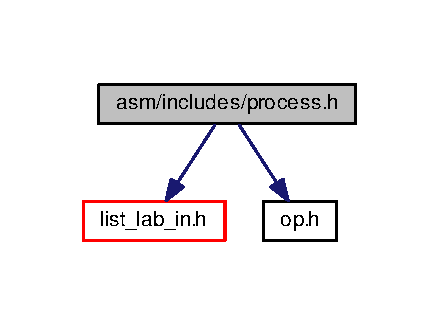
\includegraphics[width=210pt]{d5/dab/process_8h__incl}
\end{center}
\end{figure}
This graph shows which files directly or indirectly include this file\-:\nopagebreak
\begin{figure}[H]
\begin{center}
\leavevmode
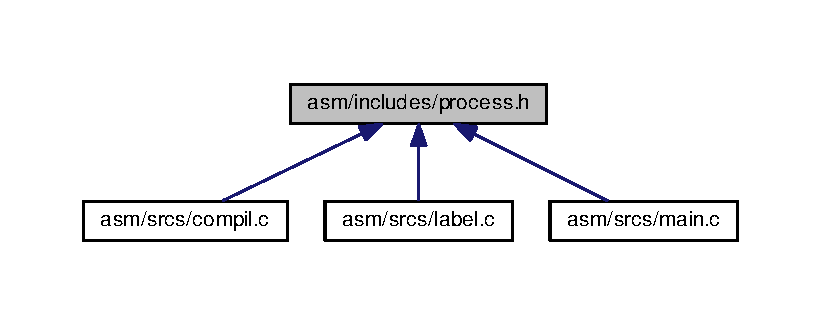
\includegraphics[width=350pt]{d1/d54/process_8h__dep__incl}
\end{center}
\end{figure}
\subsection*{Functions}
\begin{DoxyCompactItemize}
\item 
int \hyperlink{process_8h_aa60c0c2eb4c97682a8dd4be02b96072b}{process\-\_\-line} (char $\ast$$\ast$lexed\-\_\-line, int fd\-\_\-binary, int $\ast$fileoffset, \hyperlink{list__lab__in_8h_a91fca2551b14cd3e3c189afabae27a0b}{t\-\_\-lateinfo} $\ast$info)
\item 
int \hyperlink{process_8h_a7f171e754b7d166cad2b4cfe4dc9c7af}{proces\-\_\-file} (char $\ast$str)
\item 
void \hyperlink{process_8h_aec1bc88ba24446c583bfb77a27e38847}{dir\-\_\-to\-\_\-ind} (char $\ast$$\ast$lines, \hyperlink{op_8h_a51ce7549e6b9948b233d73c4c0d0fe02}{op\-\_\-t} $\ast$op)
\item 
int \hyperlink{process_8h_a22ea18f0981a9a88dcf20d45e1202143}{dirsize} (\hyperlink{op_8h_a51ce7549e6b9948b233d73c4c0d0fe02}{op\-\_\-t} $\ast$op, int i)
\end{DoxyCompactItemize}


\subsection{Function Documentation}
\hypertarget{process_8h_aec1bc88ba24446c583bfb77a27e38847}{\index{process.\-h@{process.\-h}!dir\-\_\-to\-\_\-ind@{dir\-\_\-to\-\_\-ind}}
\index{dir\-\_\-to\-\_\-ind@{dir\-\_\-to\-\_\-ind}!process.h@{process.\-h}}
\subsubsection[{dir\-\_\-to\-\_\-ind}]{\setlength{\rightskip}{0pt plus 5cm}void dir\-\_\-to\-\_\-ind (
\begin{DoxyParamCaption}
\item[{char $\ast$$\ast$}]{lines, }
\item[{{\bf op\-\_\-t} $\ast$}]{op}
\end{DoxyParamCaption}
)}}\label{process_8h_aec1bc88ba24446c583bfb77a27e38847}
\hypertarget{process_8h_a22ea18f0981a9a88dcf20d45e1202143}{\index{process.\-h@{process.\-h}!dirsize@{dirsize}}
\index{dirsize@{dirsize}!process.h@{process.\-h}}
\subsubsection[{dirsize}]{\setlength{\rightskip}{0pt plus 5cm}int dirsize (
\begin{DoxyParamCaption}
\item[{{\bf op\-\_\-t} $\ast$}]{op, }
\item[{int}]{i}
\end{DoxyParamCaption}
)}}\label{process_8h_a22ea18f0981a9a88dcf20d45e1202143}


Definition at line 100 of file process.\-c.



Here is the caller graph for this function\-:\nopagebreak
\begin{figure}[H]
\begin{center}
\leavevmode
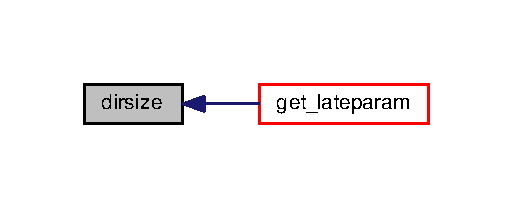
\includegraphics[width=246pt]{da/d42/process_8h_a22ea18f0981a9a88dcf20d45e1202143_icgraph}
\end{center}
\end{figure}


\hypertarget{process_8h_a7f171e754b7d166cad2b4cfe4dc9c7af}{\index{process.\-h@{process.\-h}!proces\-\_\-file@{proces\-\_\-file}}
\index{proces\-\_\-file@{proces\-\_\-file}!process.h@{process.\-h}}
\subsubsection[{proces\-\_\-file}]{\setlength{\rightskip}{0pt plus 5cm}int proces\-\_\-file (
\begin{DoxyParamCaption}
\item[{char $\ast$}]{str}
\end{DoxyParamCaption}
)}}\label{process_8h_a7f171e754b7d166cad2b4cfe4dc9c7af}


Definition at line 67 of file process.\-c.



Here is the call graph for this function\-:\nopagebreak
\begin{figure}[H]
\begin{center}
\leavevmode
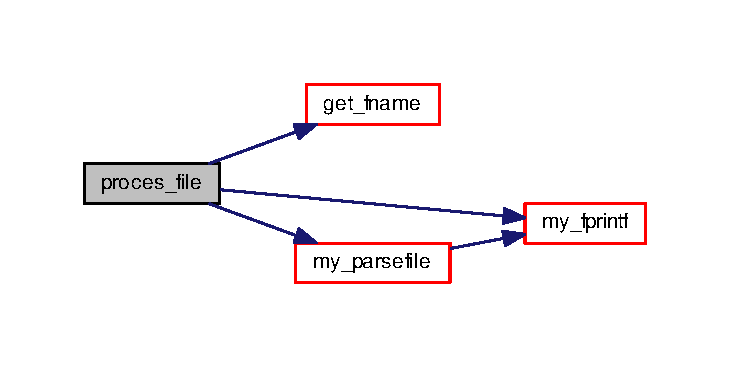
\includegraphics[width=350pt]{da/d42/process_8h_a7f171e754b7d166cad2b4cfe4dc9c7af_cgraph}
\end{center}
\end{figure}




Here is the caller graph for this function\-:\nopagebreak
\begin{figure}[H]
\begin{center}
\leavevmode
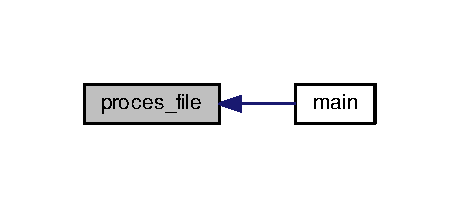
\includegraphics[width=220pt]{da/d42/process_8h_a7f171e754b7d166cad2b4cfe4dc9c7af_icgraph}
\end{center}
\end{figure}


\hypertarget{process_8h_aa60c0c2eb4c97682a8dd4be02b96072b}{\index{process.\-h@{process.\-h}!process\-\_\-line@{process\-\_\-line}}
\index{process\-\_\-line@{process\-\_\-line}!process.h@{process.\-h}}
\subsubsection[{process\-\_\-line}]{\setlength{\rightskip}{0pt plus 5cm}int process\-\_\-line (
\begin{DoxyParamCaption}
\item[{char $\ast$$\ast$}]{lexed\-\_\-line, }
\item[{int}]{fd\-\_\-binary, }
\item[{int $\ast$}]{fileoffset, }
\item[{{\bf t\-\_\-lateinfo} $\ast$}]{info}
\end{DoxyParamCaption}
)}}\label{process_8h_aa60c0c2eb4c97682a8dd4be02b96072b}


Definition at line 30 of file process.\-c.



Here is the call graph for this function\-:\nopagebreak
\begin{figure}[H]
\begin{center}
\leavevmode
\includegraphics[width=350pt]{da/d42/process_8h_aa60c0c2eb4c97682a8dd4be02b96072b_cgraph}
\end{center}
\end{figure}




Here is the caller graph for this function\-:\nopagebreak
\begin{figure}[H]
\begin{center}
\leavevmode
\includegraphics[width=264pt]{da/d42/process_8h_aa60c0c2eb4c97682a8dd4be02b96072b_icgraph}
\end{center}
\end{figure}



\hypertarget{write__argvs_8h}{\section{asm/includes/write\-\_\-argvs.h File Reference}
\label{write__argvs_8h}\index{asm/includes/write\-\_\-argvs.\-h@{asm/includes/write\-\_\-argvs.\-h}}
}
This graph shows which files directly or indirectly include this file\-:\nopagebreak
\begin{figure}[H]
\begin{center}
\leavevmode
\includegraphics[width=350pt]{da/dc6/write__argvs_8h__dep__incl}
\end{center}
\end{figure}
\subsection*{Macros}
\begin{DoxyCompactItemize}
\item 
\#define \hyperlink{write__argvs_8h_a1248d9825b1bd2636625e5bc6caf7a40}{T\-R\-U\-E\-\_\-\-R\-E\-G\-\_\-\-S\-I\-Z\-E}~1
\item 
\#define \hyperlink{write__argvs_8h_a9e00a7d6a4ed36ffa8f6d8c49e94d9eb}{T\-R\-U\-E\-\_\-\-D\-I\-R\-\_\-\-S\-I\-Z\-E}~2
\end{DoxyCompactItemize}
\subsection*{Functions}
\begin{DoxyCompactItemize}
\item 
int \hyperlink{write__argvs_8h_a83c24ebd7432a6084218b8e502bb9210}{my\-\_\-write\-\_\-arg} (int $\ast$writed, int fd\-\_\-binary, char $\ast$str, int cast)
\item 
int \hyperlink{write__argvs_8h_a929d5b863c4fbaa09c4a9fefaad3f6f4}{my\-\_\-write\-\_\-args} (char $\ast$$\ast$lexed\-\_\-line, \hyperlink{op_8h_a51ce7549e6b9948b233d73c4c0d0fe02}{op\-\_\-t} $\ast$optodo, int fd\-\_\-binary)
\item 
int \hyperlink{write__argvs_8h_ac7480a208dfb8ea7470dc43058e663e8}{write\-\_\-header} (int fd\-\_\-champ, int fd\-\_\-bin)
\item 
int \hyperlink{write__argvs_8h_ab2bbae199c6b0e2f0b46063cbd915755}{get\-\_\-name\-\_\-comment} (char $\ast$line, \hyperlink{op_8h_a4eb4dd7e74c119ccddb3032242467d65}{header\-\_\-t} $\ast$header, char $\ast$isdonename, char $\ast$isdonecom)
\item 
int \hyperlink{write__argvs_8h_a225b6690cd240c078bc78aee420e3133}{put\-\_\-in\-\_\-be} (char $\ast$arg, int size)
\item 
int \hyperlink{write__argvs_8h_a22a24dd72ba8a953542db66e3e482297}{write\-\_\-header\-\_\-ext} (int fd\-\_\-bin, int fd\-\_\-champ, \hyperlink{op_8h_a4eb4dd7e74c119ccddb3032242467d65}{header\-\_\-t} $\ast$header)
\end{DoxyCompactItemize}


\subsection{Macro Definition Documentation}
\hypertarget{write__argvs_8h_a9e00a7d6a4ed36ffa8f6d8c49e94d9eb}{\index{write\-\_\-argvs.\-h@{write\-\_\-argvs.\-h}!T\-R\-U\-E\-\_\-\-D\-I\-R\-\_\-\-S\-I\-Z\-E@{T\-R\-U\-E\-\_\-\-D\-I\-R\-\_\-\-S\-I\-Z\-E}}
\index{T\-R\-U\-E\-\_\-\-D\-I\-R\-\_\-\-S\-I\-Z\-E@{T\-R\-U\-E\-\_\-\-D\-I\-R\-\_\-\-S\-I\-Z\-E}!write_argvs.h@{write\-\_\-argvs.\-h}}
\subsubsection[{T\-R\-U\-E\-\_\-\-D\-I\-R\-\_\-\-S\-I\-Z\-E}]{\setlength{\rightskip}{0pt plus 5cm}\#define T\-R\-U\-E\-\_\-\-D\-I\-R\-\_\-\-S\-I\-Z\-E~2}}\label{write__argvs_8h_a9e00a7d6a4ed36ffa8f6d8c49e94d9eb}


Definition at line 15 of file write\-\_\-argvs.\-h.

\hypertarget{write__argvs_8h_a1248d9825b1bd2636625e5bc6caf7a40}{\index{write\-\_\-argvs.\-h@{write\-\_\-argvs.\-h}!T\-R\-U\-E\-\_\-\-R\-E\-G\-\_\-\-S\-I\-Z\-E@{T\-R\-U\-E\-\_\-\-R\-E\-G\-\_\-\-S\-I\-Z\-E}}
\index{T\-R\-U\-E\-\_\-\-R\-E\-G\-\_\-\-S\-I\-Z\-E@{T\-R\-U\-E\-\_\-\-R\-E\-G\-\_\-\-S\-I\-Z\-E}!write_argvs.h@{write\-\_\-argvs.\-h}}
\subsubsection[{T\-R\-U\-E\-\_\-\-R\-E\-G\-\_\-\-S\-I\-Z\-E}]{\setlength{\rightskip}{0pt plus 5cm}\#define T\-R\-U\-E\-\_\-\-R\-E\-G\-\_\-\-S\-I\-Z\-E~1}}\label{write__argvs_8h_a1248d9825b1bd2636625e5bc6caf7a40}


Definition at line 14 of file write\-\_\-argvs.\-h.



\subsection{Function Documentation}
\hypertarget{write__argvs_8h_ab2bbae199c6b0e2f0b46063cbd915755}{\index{write\-\_\-argvs.\-h@{write\-\_\-argvs.\-h}!get\-\_\-name\-\_\-comment@{get\-\_\-name\-\_\-comment}}
\index{get\-\_\-name\-\_\-comment@{get\-\_\-name\-\_\-comment}!write_argvs.h@{write\-\_\-argvs.\-h}}
\subsubsection[{get\-\_\-name\-\_\-comment}]{\setlength{\rightskip}{0pt plus 5cm}int get\-\_\-name\-\_\-comment (
\begin{DoxyParamCaption}
\item[{char $\ast$}]{line, }
\item[{{\bf header\-\_\-t} $\ast$}]{header, }
\item[{char $\ast$}]{isdonename, }
\item[{char $\ast$}]{isdonecom}
\end{DoxyParamCaption}
)}}\label{write__argvs_8h_ab2bbae199c6b0e2f0b46063cbd915755}


Definition at line 30 of file write\-\_\-header.\-c.



Here is the call graph for this function\-:\nopagebreak
\begin{figure}[H]
\begin{center}
\leavevmode
\includegraphics[width=350pt]{de/ddd/write__argvs_8h_ab2bbae199c6b0e2f0b46063cbd915755_cgraph}
\end{center}
\end{figure}




Here is the caller graph for this function\-:\nopagebreak
\begin{figure}[H]
\begin{center}
\leavevmode
\includegraphics[width=300pt]{de/ddd/write__argvs_8h_ab2bbae199c6b0e2f0b46063cbd915755_icgraph}
\end{center}
\end{figure}


\hypertarget{write__argvs_8h_a83c24ebd7432a6084218b8e502bb9210}{\index{write\-\_\-argvs.\-h@{write\-\_\-argvs.\-h}!my\-\_\-write\-\_\-arg@{my\-\_\-write\-\_\-arg}}
\index{my\-\_\-write\-\_\-arg@{my\-\_\-write\-\_\-arg}!write_argvs.h@{write\-\_\-argvs.\-h}}
\subsubsection[{my\-\_\-write\-\_\-arg}]{\setlength{\rightskip}{0pt plus 5cm}int my\-\_\-write\-\_\-arg (
\begin{DoxyParamCaption}
\item[{int $\ast$}]{writed, }
\item[{int}]{fd\-\_\-binary, }
\item[{char $\ast$}]{str, }
\item[{int}]{cast}
\end{DoxyParamCaption}
)}}\label{write__argvs_8h_a83c24ebd7432a6084218b8e502bb9210}


Definition at line 60 of file write\-\_\-argvs.\-c.



Here is the call graph for this function\-:\nopagebreak
\begin{figure}[H]
\begin{center}
\leavevmode
\includegraphics[width=350pt]{de/ddd/write__argvs_8h_a83c24ebd7432a6084218b8e502bb9210_cgraph}
\end{center}
\end{figure}




Here is the caller graph for this function\-:\nopagebreak
\begin{figure}[H]
\begin{center}
\leavevmode
\includegraphics[width=276pt]{de/ddd/write__argvs_8h_a83c24ebd7432a6084218b8e502bb9210_icgraph}
\end{center}
\end{figure}


\hypertarget{write__argvs_8h_a929d5b863c4fbaa09c4a9fefaad3f6f4}{\index{write\-\_\-argvs.\-h@{write\-\_\-argvs.\-h}!my\-\_\-write\-\_\-args@{my\-\_\-write\-\_\-args}}
\index{my\-\_\-write\-\_\-args@{my\-\_\-write\-\_\-args}!write_argvs.h@{write\-\_\-argvs.\-h}}
\subsubsection[{my\-\_\-write\-\_\-args}]{\setlength{\rightskip}{0pt plus 5cm}int my\-\_\-write\-\_\-args (
\begin{DoxyParamCaption}
\item[{char $\ast$$\ast$}]{lexed\-\_\-line, }
\item[{{\bf op\-\_\-t} $\ast$}]{optodo, }
\item[{int}]{fd\-\_\-binary}
\end{DoxyParamCaption}
)}}\label{write__argvs_8h_a929d5b863c4fbaa09c4a9fefaad3f6f4}


Definition at line 118 of file write\-\_\-argvs.\-c.



Here is the call graph for this function\-:\nopagebreak
\begin{figure}[H]
\begin{center}
\leavevmode
\includegraphics[width=302pt]{de/ddd/write__argvs_8h_a929d5b863c4fbaa09c4a9fefaad3f6f4_cgraph}
\end{center}
\end{figure}




Here is the caller graph for this function\-:\nopagebreak
\begin{figure}[H]
\begin{center}
\leavevmode
\includegraphics[width=264pt]{de/ddd/write__argvs_8h_a929d5b863c4fbaa09c4a9fefaad3f6f4_icgraph}
\end{center}
\end{figure}


\hypertarget{write__argvs_8h_a225b6690cd240c078bc78aee420e3133}{\index{write\-\_\-argvs.\-h@{write\-\_\-argvs.\-h}!put\-\_\-in\-\_\-be@{put\-\_\-in\-\_\-be}}
\index{put\-\_\-in\-\_\-be@{put\-\_\-in\-\_\-be}!write_argvs.h@{write\-\_\-argvs.\-h}}
\subsubsection[{put\-\_\-in\-\_\-be}]{\setlength{\rightskip}{0pt plus 5cm}int put\-\_\-in\-\_\-be (
\begin{DoxyParamCaption}
\item[{char $\ast$}]{arg, }
\item[{int}]{size}
\end{DoxyParamCaption}
)}}\label{write__argvs_8h_a225b6690cd240c078bc78aee420e3133}


Definition at line 62 of file write\-\_\-header.\-c.



Here is the call graph for this function\-:
\nopagebreak
\begin{figure}[H]
\begin{center}
\leavevmode
\includegraphics[width=242pt]{de/ddd/write__argvs_8h_a225b6690cd240c078bc78aee420e3133_cgraph}
\end{center}
\end{figure}




Here is the caller graph for this function\-:\nopagebreak
\begin{figure}[H]
\begin{center}
\leavevmode
\includegraphics[width=350pt]{de/ddd/write__argvs_8h_a225b6690cd240c078bc78aee420e3133_icgraph}
\end{center}
\end{figure}


\hypertarget{write__argvs_8h_ac7480a208dfb8ea7470dc43058e663e8}{\index{write\-\_\-argvs.\-h@{write\-\_\-argvs.\-h}!write\-\_\-header@{write\-\_\-header}}
\index{write\-\_\-header@{write\-\_\-header}!write_argvs.h@{write\-\_\-argvs.\-h}}
\subsubsection[{write\-\_\-header}]{\setlength{\rightskip}{0pt plus 5cm}int write\-\_\-header (
\begin{DoxyParamCaption}
\item[{int}]{fd\-\_\-champ, }
\item[{int}]{fd\-\_\-bin}
\end{DoxyParamCaption}
)}}\label{write__argvs_8h_ac7480a208dfb8ea7470dc43058e663e8}


Definition at line 118 of file write\-\_\-header.\-c.



Here is the call graph for this function\-:\nopagebreak
\begin{figure}[H]
\begin{center}
\leavevmode
\includegraphics[width=350pt]{de/ddd/write__argvs_8h_ac7480a208dfb8ea7470dc43058e663e8_cgraph}
\end{center}
\end{figure}




Here is the caller graph for this function\-:\nopagebreak
\begin{figure}[H]
\begin{center}
\leavevmode
\includegraphics[width=266pt]{de/ddd/write__argvs_8h_ac7480a208dfb8ea7470dc43058e663e8_icgraph}
\end{center}
\end{figure}


\hypertarget{write__argvs_8h_a22a24dd72ba8a953542db66e3e482297}{\index{write\-\_\-argvs.\-h@{write\-\_\-argvs.\-h}!write\-\_\-header\-\_\-ext@{write\-\_\-header\-\_\-ext}}
\index{write\-\_\-header\-\_\-ext@{write\-\_\-header\-\_\-ext}!write_argvs.h@{write\-\_\-argvs.\-h}}
\subsubsection[{write\-\_\-header\-\_\-ext}]{\setlength{\rightskip}{0pt plus 5cm}int write\-\_\-header\-\_\-ext (
\begin{DoxyParamCaption}
\item[{int}]{fd\-\_\-bin, }
\item[{int}]{fd\-\_\-champ, }
\item[{{\bf header\-\_\-t} $\ast$}]{header}
\end{DoxyParamCaption}
)}}\label{write__argvs_8h_a22a24dd72ba8a953542db66e3e482297}


Definition at line 92 of file write\-\_\-header.\-c.



Here is the call graph for this function\-:\nopagebreak
\begin{figure}[H]
\begin{center}
\leavevmode
\includegraphics[width=270pt]{de/ddd/write__argvs_8h_a22a24dd72ba8a953542db66e3e482297_cgraph}
\end{center}
\end{figure}




Here is the caller graph for this function\-:\nopagebreak
\begin{figure}[H]
\begin{center}
\leavevmode
\includegraphics[width=286pt]{de/ddd/write__argvs_8h_a22a24dd72ba8a953542db66e3e482297_icgraph}
\end{center}
\end{figure}



\hypertarget{check__param_8c}{\section{asm/srcs/check\-\_\-param.c File Reference}
\label{check__param_8c}\index{asm/srcs/check\-\_\-param.\-c@{asm/srcs/check\-\_\-param.\-c}}
}
{\ttfamily \#include $<$stdlib.\-h$>$}\\*
{\ttfamily \#include \char`\"{}string.\-h\char`\"{}}\\*
{\ttfamily \#include \char`\"{}compile.\-h\char`\"{}}\\*
{\ttfamily \#include \char`\"{}my\-\_\-fprintf.\-h\char`\"{}}\\*
{\ttfamily \#include \char`\"{}op.\-h\char`\"{}}\\*
Include dependency graph for check\-\_\-param.\-c\-:
\nopagebreak
\begin{figure}[H]
\begin{center}
\leavevmode
\includegraphics[width=350pt]{df/d87/check__param_8c__incl}
\end{center}
\end{figure}
\subsection*{Functions}
\begin{DoxyCompactItemize}
\item 
int \hyperlink{check__param_8c_a3733c5d12a474ef3f52f2b842588a5e9}{my\-\_\-check\-\_\-param} (\hyperlink{op_8h_a4819392a6eb5f0799ea856ae99557fba}{args\-\_\-type\-\_\-t} type, char $\ast$param)
\item 
int \hyperlink{check__param_8c_a7229d177ffd996a1f37989728c5c11d2}{my\-\_\-check\-\_\-params} (int i, \hyperlink{op_8h_a51ce7549e6b9948b233d73c4c0d0fe02}{op\-\_\-t} $\ast$op, char $\ast$$\ast$lexed\-\_\-line)
\item 
int \hyperlink{check__param_8c_a1ad3c381180e678695983d1c91157f3c}{check\-\_\-if\-\_\-valid\-\_\-label} (char $\ast$str)
\end{DoxyCompactItemize}


\subsection{Function Documentation}
\hypertarget{check__param_8c_a1ad3c381180e678695983d1c91157f3c}{\index{check\-\_\-param.\-c@{check\-\_\-param.\-c}!check\-\_\-if\-\_\-valid\-\_\-label@{check\-\_\-if\-\_\-valid\-\_\-label}}
\index{check\-\_\-if\-\_\-valid\-\_\-label@{check\-\_\-if\-\_\-valid\-\_\-label}!check_param.c@{check\-\_\-param.\-c}}
\subsubsection[{check\-\_\-if\-\_\-valid\-\_\-label}]{\setlength{\rightskip}{0pt plus 5cm}int check\-\_\-if\-\_\-valid\-\_\-label (
\begin{DoxyParamCaption}
\item[{char $\ast$}]{str}
\end{DoxyParamCaption}
)}}\label{check__param_8c_a1ad3c381180e678695983d1c91157f3c}


Definition at line 74 of file check\-\_\-param.\-c.



Here is the call graph for this function\-:\nopagebreak
\begin{figure}[H]
\begin{center}
\leavevmode
\includegraphics[width=282pt]{de/d36/check__param_8c_a1ad3c381180e678695983d1c91157f3c_cgraph}
\end{center}
\end{figure}




Here is the caller graph for this function\-:\nopagebreak
\begin{figure}[H]
\begin{center}
\leavevmode
\includegraphics[width=302pt]{de/d36/check__param_8c_a1ad3c381180e678695983d1c91157f3c_icgraph}
\end{center}
\end{figure}


\hypertarget{check__param_8c_a3733c5d12a474ef3f52f2b842588a5e9}{\index{check\-\_\-param.\-c@{check\-\_\-param.\-c}!my\-\_\-check\-\_\-param@{my\-\_\-check\-\_\-param}}
\index{my\-\_\-check\-\_\-param@{my\-\_\-check\-\_\-param}!check_param.c@{check\-\_\-param.\-c}}
\subsubsection[{my\-\_\-check\-\_\-param}]{\setlength{\rightskip}{0pt plus 5cm}int my\-\_\-check\-\_\-param (
\begin{DoxyParamCaption}
\item[{{\bf args\-\_\-type\-\_\-t}}]{type, }
\item[{char $\ast$}]{param}
\end{DoxyParamCaption}
)}}\label{check__param_8c_a3733c5d12a474ef3f52f2b842588a5e9}


Definition at line 21 of file check\-\_\-param.\-c.



Here is the call graph for this function\-:\nopagebreak
\begin{figure}[H]
\begin{center}
\leavevmode
\includegraphics[width=270pt]{de/d36/check__param_8c_a3733c5d12a474ef3f52f2b842588a5e9_cgraph}
\end{center}
\end{figure}




Here is the caller graph for this function\-:\nopagebreak
\begin{figure}[H]
\begin{center}
\leavevmode
\includegraphics[width=314pt]{de/d36/check__param_8c_a3733c5d12a474ef3f52f2b842588a5e9_icgraph}
\end{center}
\end{figure}


\hypertarget{check__param_8c_a7229d177ffd996a1f37989728c5c11d2}{\index{check\-\_\-param.\-c@{check\-\_\-param.\-c}!my\-\_\-check\-\_\-params@{my\-\_\-check\-\_\-params}}
\index{my\-\_\-check\-\_\-params@{my\-\_\-check\-\_\-params}!check_param.c@{check\-\_\-param.\-c}}
\subsubsection[{my\-\_\-check\-\_\-params}]{\setlength{\rightskip}{0pt plus 5cm}int my\-\_\-check\-\_\-params (
\begin{DoxyParamCaption}
\item[{int}]{i, }
\item[{{\bf op\-\_\-t} $\ast$}]{op, }
\item[{char $\ast$$\ast$}]{lexed\-\_\-line}
\end{DoxyParamCaption}
)}}\label{check__param_8c_a7229d177ffd996a1f37989728c5c11d2}


Definition at line 48 of file check\-\_\-param.\-c.



Here is the call graph for this function\-:\nopagebreak
\begin{figure}[H]
\begin{center}
\leavevmode
\includegraphics[width=350pt]{de/d36/check__param_8c_a7229d177ffd996a1f37989728c5c11d2_cgraph}
\end{center}
\end{figure}




Here is the caller graph for this function\-:\nopagebreak
\begin{figure}[H]
\begin{center}
\leavevmode
\includegraphics[width=284pt]{de/d36/check__param_8c_a7229d177ffd996a1f37989728c5c11d2_icgraph}
\end{center}
\end{figure}



\hypertarget{compil_8c}{\section{asm/srcs/compil.c File Reference}
\label{compil_8c}\index{asm/srcs/compil.\-c@{asm/srcs/compil.\-c}}
}
{\ttfamily \#include $<$unistd.\-h$>$}\\*
{\ttfamily \#include \char`\"{}stdlib.\-h\char`\"{}}\\*
{\ttfamily \#include \char`\"{}list\-\_\-lab\-\_\-in.\-h\char`\"{}}\\*
{\ttfamily \#include \char`\"{}process.\-h\char`\"{}}\\*
{\ttfamily \#include \char`\"{}get\-\_\-next\-\_\-line.\-h\char`\"{}}\\*
{\ttfamily \#include \char`\"{}my\-\_\-fprintf.\-h\char`\"{}}\\*
{\ttfamily \#include \char`\"{}op.\-h\char`\"{}}\\*
{\ttfamily \#include \char`\"{}string.\-h\char`\"{}}\\*
{\ttfamily \#include \char`\"{}my\-\_\-malloc.\-h\char`\"{}}\\*
{\ttfamily \#include \char`\"{}check.\-h\char`\"{}}\\*
{\ttfamily \#include \char`\"{}write\-\_\-argvs.\-h\char`\"{}}\\*
{\ttfamily \#include \char`\"{}lexer.\-h\char`\"{}}\\*
{\ttfamily \#include \char`\"{}compile.\-h\char`\"{}}\\*
Include dependency graph for compil.\-c\-:
\nopagebreak
\begin{figure}[H]
\begin{center}
\leavevmode
\includegraphics[width=350pt]{d3/dbb/compil_8c__incl}
\end{center}
\end{figure}
\subsection*{Functions}
\begin{DoxyCompactItemize}
\item 
int \hyperlink{compil_8c_ac90570dbce495f89534c76073a2c1831}{my\-\_\-compil} (char $\ast$$\ast$lexed\-\_\-line, \hyperlink{op_8h_a51ce7549e6b9948b233d73c4c0d0fe02}{op\-\_\-t} $\ast$optodo, int fd\-\_\-binary)
\item 
void \hyperlink{compil_8c_a4131ae481061ef0ee9686787e38e982d}{my\-\_\-init\-\_\-info} (\hyperlink{list__lab__in_8h_a91fca2551b14cd3e3c189afabae27a0b}{t\-\_\-lateinfo} $\ast$info)
\item 
char $\ast$$\ast$ \hyperlink{compil_8c_a81c29d4b2a8c6c27669b08812ab4e1a7}{my\-\_\-epur} (char $\ast$$\ast$tab)
\item 
int \hyperlink{compil_8c_ae9aa8d794f6c75aa3c6b131a15fcb7ca}{my\-\_\-parsefile} (int fd\-\_\-champ, int fd\-\_\-binary)
\end{DoxyCompactItemize}


\subsection{Function Documentation}
\hypertarget{compil_8c_ac90570dbce495f89534c76073a2c1831}{\index{compil.\-c@{compil.\-c}!my\-\_\-compil@{my\-\_\-compil}}
\index{my\-\_\-compil@{my\-\_\-compil}!compil.c@{compil.\-c}}
\subsubsection[{my\-\_\-compil}]{\setlength{\rightskip}{0pt plus 5cm}int my\-\_\-compil (
\begin{DoxyParamCaption}
\item[{char $\ast$$\ast$}]{lexed\-\_\-line, }
\item[{{\bf op\-\_\-t} $\ast$}]{optodo, }
\item[{int}]{fd\-\_\-binary}
\end{DoxyParamCaption}
)}}\label{compil_8c_ac90570dbce495f89534c76073a2c1831}


Definition at line 33 of file compil.\-c.



Here is the call graph for this function\-:\nopagebreak
\begin{figure}[H]
\begin{center}
\leavevmode
\includegraphics[width=350pt]{d1/d21/compil_8c_ac90570dbce495f89534c76073a2c1831_cgraph}
\end{center}
\end{figure}




Here is the caller graph for this function\-:\nopagebreak
\begin{figure}[H]
\begin{center}
\leavevmode
\includegraphics[width=256pt]{d1/d21/compil_8c_ac90570dbce495f89534c76073a2c1831_icgraph}
\end{center}
\end{figure}


\hypertarget{compil_8c_a81c29d4b2a8c6c27669b08812ab4e1a7}{\index{compil.\-c@{compil.\-c}!my\-\_\-epur@{my\-\_\-epur}}
\index{my\-\_\-epur@{my\-\_\-epur}!compil.c@{compil.\-c}}
\subsubsection[{my\-\_\-epur}]{\setlength{\rightskip}{0pt plus 5cm}char$\ast$$\ast$ my\-\_\-epur (
\begin{DoxyParamCaption}
\item[{char $\ast$$\ast$}]{tab}
\end{DoxyParamCaption}
)}}\label{compil_8c_a81c29d4b2a8c6c27669b08812ab4e1a7}


Definition at line 74 of file compil.\-c.



Here is the caller graph for this function\-:\nopagebreak
\begin{figure}[H]
\begin{center}
\leavevmode
\includegraphics[width=246pt]{d1/d21/compil_8c_a81c29d4b2a8c6c27669b08812ab4e1a7_icgraph}
\end{center}
\end{figure}


\hypertarget{compil_8c_a4131ae481061ef0ee9686787e38e982d}{\index{compil.\-c@{compil.\-c}!my\-\_\-init\-\_\-info@{my\-\_\-init\-\_\-info}}
\index{my\-\_\-init\-\_\-info@{my\-\_\-init\-\_\-info}!compil.c@{compil.\-c}}
\subsubsection[{my\-\_\-init\-\_\-info}]{\setlength{\rightskip}{0pt plus 5cm}void my\-\_\-init\-\_\-info (
\begin{DoxyParamCaption}
\item[{{\bf t\-\_\-lateinfo} $\ast$}]{info}
\end{DoxyParamCaption}
)}}\label{compil_8c_a4131ae481061ef0ee9686787e38e982d}


Definition at line 61 of file compil.\-c.



Here is the caller graph for this function\-:\nopagebreak
\begin{figure}[H]
\begin{center}
\leavevmode
\includegraphics[width=258pt]{d1/d21/compil_8c_a4131ae481061ef0ee9686787e38e982d_icgraph}
\end{center}
\end{figure}


\hypertarget{compil_8c_ae9aa8d794f6c75aa3c6b131a15fcb7ca}{\index{compil.\-c@{compil.\-c}!my\-\_\-parsefile@{my\-\_\-parsefile}}
\index{my\-\_\-parsefile@{my\-\_\-parsefile}!compil.c@{compil.\-c}}
\subsubsection[{my\-\_\-parsefile}]{\setlength{\rightskip}{0pt plus 5cm}int my\-\_\-parsefile (
\begin{DoxyParamCaption}
\item[{int}]{fd\-\_\-champ, }
\item[{int}]{fd\-\_\-binary}
\end{DoxyParamCaption}
)}}\label{compil_8c_ae9aa8d794f6c75aa3c6b131a15fcb7ca}


Definition at line 113 of file compil.\-c.



Here is the call graph for this function\-:
\nopagebreak
\begin{figure}[H]
\begin{center}
\leavevmode
\includegraphics[width=350pt]{d1/d21/compil_8c_ae9aa8d794f6c75aa3c6b131a15fcb7ca_cgraph}
\end{center}
\end{figure}




Here is the caller graph for this function\-:\nopagebreak
\begin{figure}[H]
\begin{center}
\leavevmode
\includegraphics[width=256pt]{d1/d21/compil_8c_ae9aa8d794f6c75aa3c6b131a15fcb7ca_icgraph}
\end{center}
\end{figure}



\hypertarget{gen__list_8c}{\section{asm/srcs/gen\-\_\-list.c File Reference}
\label{gen__list_8c}\index{asm/srcs/gen\-\_\-list.\-c@{asm/srcs/gen\-\_\-list.\-c}}
}
{\ttfamily \#include $<$stdlib.\-h$>$}\\*
{\ttfamily \#include \char`\"{}gen\-\_\-list.\-h\char`\"{}}\\*
{\ttfamily \#include \char`\"{}string.\-h\char`\"{}}\\*
{\ttfamily \#include \char`\"{}string\-\_\-compare.\-h\char`\"{}}\\*
{\ttfamily \#include \char`\"{}op.\-h\char`\"{}}\\*
Include dependency graph for gen\-\_\-list.\-c\-:
\nopagebreak
\begin{figure}[H]
\begin{center}
\leavevmode
\includegraphics[width=350pt]{d3/d81/gen__list_8c__incl}
\end{center}
\end{figure}
\subsection*{Functions}
\begin{DoxyCompactItemize}
\item 
\hyperlink{gen__list_8h_aefde00352c5326bb1c28ebd4404c4795}{t\-\_\-list} $\ast$ \hyperlink{gen__list_8c_a996418ddda561236678a0d866b0ae06a}{new\-\_\-list} (\hyperlink{gen__list_8h_aefde00352c5326bb1c28ebd4404c4795}{t\-\_\-list} $\ast$old, int num\-\_\-a, int num\-\_\-b, char $\ast$str)
\item 
void \hyperlink{gen__list_8c_a20852ea164cf7011db3e0ba5367f40ca}{free\-\_\-list} (\hyperlink{gen__list_8h_aefde00352c5326bb1c28ebd4404c4795}{t\-\_\-list} $\ast$s)
\item 
int \hyperlink{gen__list_8c_a2dfa3098ff9d3cf0f38ab89d1502463f}{my\-\_\-strcmp\-\_\-lab} (char $\ast$label, char $\ast$str)
\item 
int \hyperlink{gen__list_8c_a34fcfee2bee8985bfd57e10d1ac7b47a}{list\-\_\-finder} (\hyperlink{gen__list_8h_aefde00352c5326bb1c28ebd4404c4795}{t\-\_\-list} $\ast$s, char $\ast$label)
\end{DoxyCompactItemize}


\subsection{Function Documentation}
\hypertarget{gen__list_8c_a20852ea164cf7011db3e0ba5367f40ca}{\index{gen\-\_\-list.\-c@{gen\-\_\-list.\-c}!free\-\_\-list@{free\-\_\-list}}
\index{free\-\_\-list@{free\-\_\-list}!gen_list.c@{gen\-\_\-list.\-c}}
\subsubsection[{free\-\_\-list}]{\setlength{\rightskip}{0pt plus 5cm}void free\-\_\-list (
\begin{DoxyParamCaption}
\item[{{\bf t\-\_\-list} $\ast$}]{s}
\end{DoxyParamCaption}
)}}\label{gen__list_8c_a20852ea164cf7011db3e0ba5367f40ca}


Definition at line 47 of file gen\-\_\-list.\-c.

\hypertarget{gen__list_8c_a34fcfee2bee8985bfd57e10d1ac7b47a}{\index{gen\-\_\-list.\-c@{gen\-\_\-list.\-c}!list\-\_\-finder@{list\-\_\-finder}}
\index{list\-\_\-finder@{list\-\_\-finder}!gen_list.c@{gen\-\_\-list.\-c}}
\subsubsection[{list\-\_\-finder}]{\setlength{\rightskip}{0pt plus 5cm}int list\-\_\-finder (
\begin{DoxyParamCaption}
\item[{{\bf t\-\_\-list} $\ast$}]{s, }
\item[{char $\ast$}]{label}
\end{DoxyParamCaption}
)}}\label{gen__list_8c_a34fcfee2bee8985bfd57e10d1ac7b47a}


Definition at line 91 of file gen\-\_\-list.\-c.



Here is the call graph for this function\-:
\nopagebreak
\begin{figure}[H]
\begin{center}
\leavevmode
\includegraphics[width=260pt]{d0/db6/gen__list_8c_a34fcfee2bee8985bfd57e10d1ac7b47a_cgraph}
\end{center}
\end{figure}




Here is the caller graph for this function\-:\nopagebreak
\begin{figure}[H]
\begin{center}
\leavevmode
\includegraphics[width=256pt]{d0/db6/gen__list_8c_a34fcfee2bee8985bfd57e10d1ac7b47a_icgraph}
\end{center}
\end{figure}


\hypertarget{gen__list_8c_a2dfa3098ff9d3cf0f38ab89d1502463f}{\index{gen\-\_\-list.\-c@{gen\-\_\-list.\-c}!my\-\_\-strcmp\-\_\-lab@{my\-\_\-strcmp\-\_\-lab}}
\index{my\-\_\-strcmp\-\_\-lab@{my\-\_\-strcmp\-\_\-lab}!gen_list.c@{gen\-\_\-list.\-c}}
\subsubsection[{my\-\_\-strcmp\-\_\-lab}]{\setlength{\rightskip}{0pt plus 5cm}int my\-\_\-strcmp\-\_\-lab (
\begin{DoxyParamCaption}
\item[{char $\ast$}]{label, }
\item[{char $\ast$}]{str}
\end{DoxyParamCaption}
)}}\label{gen__list_8c_a2dfa3098ff9d3cf0f38ab89d1502463f}


Definition at line 68 of file gen\-\_\-list.\-c.



Here is the call graph for this function\-:
\nopagebreak
\begin{figure}[H]
\begin{center}
\leavevmode
\includegraphics[width=260pt]{d0/db6/gen__list_8c_a2dfa3098ff9d3cf0f38ab89d1502463f_cgraph}
\end{center}
\end{figure}




Here is the caller graph for this function\-:\nopagebreak
\begin{figure}[H]
\begin{center}
\leavevmode
\includegraphics[width=260pt]{d0/db6/gen__list_8c_a2dfa3098ff9d3cf0f38ab89d1502463f_icgraph}
\end{center}
\end{figure}


\hypertarget{gen__list_8c_a996418ddda561236678a0d866b0ae06a}{\index{gen\-\_\-list.\-c@{gen\-\_\-list.\-c}!new\-\_\-list@{new\-\_\-list}}
\index{new\-\_\-list@{new\-\_\-list}!gen_list.c@{gen\-\_\-list.\-c}}
\subsubsection[{new\-\_\-list}]{\setlength{\rightskip}{0pt plus 5cm}{\bf t\-\_\-list}$\ast$ new\-\_\-list (
\begin{DoxyParamCaption}
\item[{{\bf t\-\_\-list} $\ast$}]{old, }
\item[{int}]{num\-\_\-a, }
\item[{int}]{num\-\_\-b, }
\item[{char $\ast$}]{str}
\end{DoxyParamCaption}
)}}\label{gen__list_8c_a996418ddda561236678a0d866b0ae06a}


Definition at line 22 of file gen\-\_\-list.\-c.



Here is the caller graph for this function\-:\nopagebreak
\begin{figure}[H]
\begin{center}
\leavevmode
\includegraphics[width=248pt]{d0/db6/gen__list_8c_a996418ddda561236678a0d866b0ae06a_icgraph}
\end{center}
\end{figure}



\hypertarget{get__argv_8c}{\section{asm/srcs/get\-\_\-argv.c File Reference}
\label{get__argv_8c}\index{asm/srcs/get\-\_\-argv.\-c@{asm/srcs/get\-\_\-argv.\-c}}
}
{\ttfamily \#include $<$stdlib.\-h$>$}\\*
{\ttfamily \#include \char`\"{}string\-\_\-compare.\-h\char`\"{}}\\*
{\ttfamily \#include \char`\"{}my\-\_\-fprintf.\-h\char`\"{}}\\*
{\ttfamily \#include \char`\"{}string\-\_\-copy.\-h\char`\"{}}\\*
{\ttfamily \#include \char`\"{}string.\-h\char`\"{}}\\*
{\ttfamily \#include \char`\"{}op.\-h\char`\"{}}\\*
{\ttfamily \#include \char`\"{}compile.\-h\char`\"{}}\\*
Include dependency graph for get\-\_\-argv.\-c\-:
\nopagebreak
\begin{figure}[H]
\begin{center}
\leavevmode
\includegraphics[width=350pt]{d4/d71/get__argv_8c__incl}
\end{center}
\end{figure}
\subsection*{Functions}
\begin{DoxyCompactItemize}
\item 
char $\ast$ \hyperlink{get__argv_8c_a0b2ae2ba08582e01f1fa3a02a42e4014}{get\-\_\-fname} (char $\ast$fname, char $\ast$str)
\item 
char $\ast$ \hyperlink{get__argv_8c_a91d9889f105aba2ceba52a0554c4d872}{get\-\_\-quotes\-\_\-comment} (const char $\ast$str, char ret\mbox{[}$\,$\mbox{]})
\item 
char $\ast$ \hyperlink{get__argv_8c_a4e291b57bd0c553d7bbad7f3e5b7cd50}{get\-\_\-quotes\-\_\-name} (const char $\ast$str, char ret\mbox{[}$\,$\mbox{]})
\end{DoxyCompactItemize}


\subsection{Function Documentation}
\hypertarget{get__argv_8c_a0b2ae2ba08582e01f1fa3a02a42e4014}{\index{get\-\_\-argv.\-c@{get\-\_\-argv.\-c}!get\-\_\-fname@{get\-\_\-fname}}
\index{get\-\_\-fname@{get\-\_\-fname}!get_argv.c@{get\-\_\-argv.\-c}}
\subsubsection[{get\-\_\-fname}]{\setlength{\rightskip}{0pt plus 5cm}char$\ast$ get\-\_\-fname (
\begin{DoxyParamCaption}
\item[{char $\ast$}]{fname, }
\item[{char $\ast$}]{str}
\end{DoxyParamCaption}
)}}\label{get__argv_8c_a0b2ae2ba08582e01f1fa3a02a42e4014}


Definition at line 24 of file get\-\_\-argv.\-c.



Here is the call graph for this function\-:\nopagebreak
\begin{figure}[H]
\begin{center}
\leavevmode
\includegraphics[width=246pt]{db/da1/get__argv_8c_a0b2ae2ba08582e01f1fa3a02a42e4014_cgraph}
\end{center}
\end{figure}




Here is the caller graph for this function\-:\nopagebreak
\begin{figure}[H]
\begin{center}
\leavevmode
\includegraphics[width=246pt]{db/da1/get__argv_8c_a0b2ae2ba08582e01f1fa3a02a42e4014_icgraph}
\end{center}
\end{figure}


\hypertarget{get__argv_8c_a91d9889f105aba2ceba52a0554c4d872}{\index{get\-\_\-argv.\-c@{get\-\_\-argv.\-c}!get\-\_\-quotes\-\_\-comment@{get\-\_\-quotes\-\_\-comment}}
\index{get\-\_\-quotes\-\_\-comment@{get\-\_\-quotes\-\_\-comment}!get_argv.c@{get\-\_\-argv.\-c}}
\subsubsection[{get\-\_\-quotes\-\_\-comment}]{\setlength{\rightskip}{0pt plus 5cm}char$\ast$ get\-\_\-quotes\-\_\-comment (
\begin{DoxyParamCaption}
\item[{const char $\ast$}]{str, }
\item[{char}]{ret\mbox{[}$\,$\mbox{]}}
\end{DoxyParamCaption}
)}}\label{get__argv_8c_a91d9889f105aba2ceba52a0554c4d872}


Definition at line 45 of file get\-\_\-argv.\-c.



Here is the call graph for this function\-:\nopagebreak
\begin{figure}[H]
\begin{center}
\leavevmode
\includegraphics[width=288pt]{db/da1/get__argv_8c_a91d9889f105aba2ceba52a0554c4d872_cgraph}
\end{center}
\end{figure}




Here is the caller graph for this function\-:\nopagebreak
\begin{figure}[H]
\begin{center}
\leavevmode
\includegraphics[width=338pt]{db/da1/get__argv_8c_a91d9889f105aba2ceba52a0554c4d872_icgraph}
\end{center}
\end{figure}


\hypertarget{get__argv_8c_a4e291b57bd0c553d7bbad7f3e5b7cd50}{\index{get\-\_\-argv.\-c@{get\-\_\-argv.\-c}!get\-\_\-quotes\-\_\-name@{get\-\_\-quotes\-\_\-name}}
\index{get\-\_\-quotes\-\_\-name@{get\-\_\-quotes\-\_\-name}!get_argv.c@{get\-\_\-argv.\-c}}
\subsubsection[{get\-\_\-quotes\-\_\-name}]{\setlength{\rightskip}{0pt plus 5cm}char$\ast$ get\-\_\-quotes\-\_\-name (
\begin{DoxyParamCaption}
\item[{const char $\ast$}]{str, }
\item[{char}]{ret\mbox{[}$\,$\mbox{]}}
\end{DoxyParamCaption}
)}}\label{get__argv_8c_a4e291b57bd0c553d7bbad7f3e5b7cd50}


Definition at line 79 of file get\-\_\-argv.\-c.



Here is the call graph for this function\-:\nopagebreak
\begin{figure}[H]
\begin{center}
\leavevmode
\includegraphics[width=272pt]{db/da1/get__argv_8c_a4e291b57bd0c553d7bbad7f3e5b7cd50_cgraph}
\end{center}
\end{figure}




Here is the caller graph for this function\-:\nopagebreak
\begin{figure}[H]
\begin{center}
\leavevmode
\includegraphics[width=322pt]{db/da1/get__argv_8c_a4e291b57bd0c553d7bbad7f3e5b7cd50_icgraph}
\end{center}
\end{figure}



\hypertarget{label_8c}{\section{asm/srcs/label.c File Reference}
\label{label_8c}\index{asm/srcs/label.\-c@{asm/srcs/label.\-c}}
}
{\ttfamily \#include $<$unistd.\-h$>$}\\*
{\ttfamily \#include $<$fcntl.\-h$>$}\\*
{\ttfamily \#include $<$sys/stat.\-h$>$}\\*
{\ttfamily \#include \char`\"{}op.\-h\char`\"{}}\\*
{\ttfamily \#include \char`\"{}list\-\_\-lab\-\_\-in.\-h\char`\"{}}\\*
{\ttfamily \#include \char`\"{}get\-\_\-argv.\-h\char`\"{}}\\*
{\ttfamily \#include \char`\"{}compile.\-h\char`\"{}}\\*
{\ttfamily \#include \char`\"{}string\-\_\-copy.\-h\char`\"{}}\\*
{\ttfamily \#include \char`\"{}my\-\_\-fprintf.\-h\char`\"{}}\\*
{\ttfamily \#include \char`\"{}write\-\_\-argvs.\-h\char`\"{}}\\*
{\ttfamily \#include \char`\"{}string\-\_\-compare.\-h\char`\"{}}\\*
{\ttfamily \#include \char`\"{}my\-\_\-malloc.\-h\char`\"{}}\\*
{\ttfamily \#include \char`\"{}get\-\_\-next\-\_\-line.\-h\char`\"{}}\\*
{\ttfamily \#include \char`\"{}process.\-h\char`\"{}}\\*
{\ttfamily \#include \char`\"{}string.\-h\char`\"{}}\\*
Include dependency graph for label.\-c\-:
\nopagebreak
\begin{figure}[H]
\begin{center}
\leavevmode
\includegraphics[width=350pt]{dd/d21/label_8c__incl}
\end{center}
\end{figure}
\subsection*{Functions}
\begin{DoxyCompactItemize}
\item 
int \hyperlink{label_8c_a07317474f4f23ef25856daa71b8534da}{header\-\_\-size\-\_\-prog} (int fd\-\_\-bin, int writed)
\item 
int \hyperlink{label_8c_af66636c0f888f33983f6630fa1911bae}{late\-\_\-operation} (int fd\-\_\-bin, int writed, \hyperlink{list__lab__in_8h_a91fca2551b14cd3e3c189afabae27a0b}{t\-\_\-lateinfo} $\ast$info)
\item 
int \hyperlink{label_8c_a68e75f6dc19bf1ad207e4ede39a78a91}{get\-\_\-label\-\_\-def} (\hyperlink{list__lab__in_8h_a91fca2551b14cd3e3c189afabae27a0b}{t\-\_\-lateinfo} $\ast$info, char $\ast$$\ast$lexed\-\_\-line, int fileoffset)
\item 
int \hyperlink{label_8c_ad53c1fbf1e76c5dd094c957427c0995b}{late\-\_\-ext} (\hyperlink{list__lab__in_8h_a91fca2551b14cd3e3c189afabae27a0b}{t\-\_\-lateinfo} $\ast$info, char $\ast$word, int size, \hyperlink{compile_8h_a55d668897c420e8b402208277c8fc669}{t\-\_\-pos\-\_\-info} pos)
\item 
int \hyperlink{label_8c_a1a00bb23ce6bee936b9b966e61fba574}{get\-\_\-lateparam} (\hyperlink{list__lab__in_8h_a91fca2551b14cd3e3c189afabae27a0b}{t\-\_\-lateinfo} $\ast$info, char $\ast$$\ast$lines, int offset, \hyperlink{op_8h_a51ce7549e6b9948b233d73c4c0d0fe02}{op\-\_\-t} $\ast$op)
\end{DoxyCompactItemize}


\subsection{Function Documentation}
\hypertarget{label_8c_a68e75f6dc19bf1ad207e4ede39a78a91}{\index{label.\-c@{label.\-c}!get\-\_\-label\-\_\-def@{get\-\_\-label\-\_\-def}}
\index{get\-\_\-label\-\_\-def@{get\-\_\-label\-\_\-def}!label.c@{label.\-c}}
\subsubsection[{get\-\_\-label\-\_\-def}]{\setlength{\rightskip}{0pt plus 5cm}int get\-\_\-label\-\_\-def (
\begin{DoxyParamCaption}
\item[{{\bf t\-\_\-lateinfo} $\ast$}]{info, }
\item[{char $\ast$$\ast$}]{lexed\-\_\-line, }
\item[{int}]{fileoffset}
\end{DoxyParamCaption}
)}}\label{label_8c_a68e75f6dc19bf1ad207e4ede39a78a91}


Definition at line 84 of file label.\-c.



Here is the call graph for this function\-:\nopagebreak
\begin{figure}[H]
\begin{center}
\leavevmode
\includegraphics[width=302pt]{dc/d7e/label_8c_a68e75f6dc19bf1ad207e4ede39a78a91_cgraph}
\end{center}
\end{figure}




Here is the caller graph for this function\-:\nopagebreak
\begin{figure}[H]
\begin{center}
\leavevmode
\includegraphics[width=268pt]{dc/d7e/label_8c_a68e75f6dc19bf1ad207e4ede39a78a91_icgraph}
\end{center}
\end{figure}


\hypertarget{label_8c_a1a00bb23ce6bee936b9b966e61fba574}{\index{label.\-c@{label.\-c}!get\-\_\-lateparam@{get\-\_\-lateparam}}
\index{get\-\_\-lateparam@{get\-\_\-lateparam}!label.c@{label.\-c}}
\subsubsection[{get\-\_\-lateparam}]{\setlength{\rightskip}{0pt plus 5cm}int get\-\_\-lateparam (
\begin{DoxyParamCaption}
\item[{{\bf t\-\_\-lateinfo} $\ast$}]{info, }
\item[{char $\ast$$\ast$}]{lines, }
\item[{int}]{offset, }
\item[{{\bf op\-\_\-t} $\ast$}]{op}
\end{DoxyParamCaption}
)}}\label{label_8c_a1a00bb23ce6bee936b9b966e61fba574}


Definition at line 143 of file label.\-c.



Here is the call graph for this function\-:\nopagebreak
\begin{figure}[H]
\begin{center}
\leavevmode
\includegraphics[width=252pt]{dc/d7e/label_8c_a1a00bb23ce6bee936b9b966e61fba574_cgraph}
\end{center}
\end{figure}




Here is the caller graph for this function\-:\nopagebreak
\begin{figure}[H]
\begin{center}
\leavevmode
\includegraphics[width=272pt]{dc/d7e/label_8c_a1a00bb23ce6bee936b9b966e61fba574_icgraph}
\end{center}
\end{figure}


\hypertarget{label_8c_a07317474f4f23ef25856daa71b8534da}{\index{label.\-c@{label.\-c}!header\-\_\-size\-\_\-prog@{header\-\_\-size\-\_\-prog}}
\index{header\-\_\-size\-\_\-prog@{header\-\_\-size\-\_\-prog}!label.c@{label.\-c}}
\subsubsection[{header\-\_\-size\-\_\-prog}]{\setlength{\rightskip}{0pt plus 5cm}int header\-\_\-size\-\_\-prog (
\begin{DoxyParamCaption}
\item[{int}]{fd\-\_\-bin, }
\item[{int}]{writed}
\end{DoxyParamCaption}
)}}\label{label_8c_a07317474f4f23ef25856daa71b8534da}


Definition at line 31 of file label.\-c.



Here is the call graph for this function\-:\nopagebreak
\begin{figure}[H]
\begin{center}
\leavevmode
\includegraphics[width=274pt]{dc/d7e/label_8c_a07317474f4f23ef25856daa71b8534da_cgraph}
\end{center}
\end{figure}




Here is the caller graph for this function\-:\nopagebreak
\begin{figure}[H]
\begin{center}
\leavevmode
\includegraphics[width=294pt]{dc/d7e/label_8c_a07317474f4f23ef25856daa71b8534da_icgraph}
\end{center}
\end{figure}


\hypertarget{label_8c_ad53c1fbf1e76c5dd094c957427c0995b}{\index{label.\-c@{label.\-c}!late\-\_\-ext@{late\-\_\-ext}}
\index{late\-\_\-ext@{late\-\_\-ext}!label.c@{label.\-c}}
\subsubsection[{late\-\_\-ext}]{\setlength{\rightskip}{0pt plus 5cm}int late\-\_\-ext (
\begin{DoxyParamCaption}
\item[{{\bf t\-\_\-lateinfo} $\ast$}]{info, }
\item[{char $\ast$}]{word, }
\item[{int}]{size, }
\item[{{\bf t\-\_\-pos\-\_\-info}}]{pos}
\end{DoxyParamCaption}
)}}\label{label_8c_ad53c1fbf1e76c5dd094c957427c0995b}


Definition at line 113 of file label.\-c.



Here is the call graph for this function\-:\nopagebreak
\begin{figure}[H]
\begin{center}
\leavevmode
\includegraphics[width=234pt]{dc/d7e/label_8c_ad53c1fbf1e76c5dd094c957427c0995b_cgraph}
\end{center}
\end{figure}




Here is the caller graph for this function\-:\nopagebreak
\begin{figure}[H]
\begin{center}
\leavevmode
\includegraphics[width=250pt]{dc/d7e/label_8c_ad53c1fbf1e76c5dd094c957427c0995b_icgraph}
\end{center}
\end{figure}


\hypertarget{label_8c_af66636c0f888f33983f6630fa1911bae}{\index{label.\-c@{label.\-c}!late\-\_\-operation@{late\-\_\-operation}}
\index{late\-\_\-operation@{late\-\_\-operation}!label.c@{label.\-c}}
\subsubsection[{late\-\_\-operation}]{\setlength{\rightskip}{0pt plus 5cm}int late\-\_\-operation (
\begin{DoxyParamCaption}
\item[{int}]{fd\-\_\-bin, }
\item[{int}]{writed, }
\item[{{\bf t\-\_\-lateinfo} $\ast$}]{info}
\end{DoxyParamCaption}
)}}\label{label_8c_af66636c0f888f33983f6630fa1911bae}


Definition at line 50 of file label.\-c.



Here is the call graph for this function\-:\nopagebreak
\begin{figure}[H]
\begin{center}
\leavevmode
\includegraphics[width=350pt]{dc/d7e/label_8c_af66636c0f888f33983f6630fa1911bae_cgraph}
\end{center}
\end{figure}




Here is the caller graph for this function\-:\nopagebreak
\begin{figure}[H]
\begin{center}
\leavevmode
\includegraphics[width=270pt]{dc/d7e/label_8c_af66636c0f888f33983f6630fa1911bae_icgraph}
\end{center}
\end{figure}



\hypertarget{lexer_8c}{\section{asm/srcs/lexer.c File Reference}
\label{lexer_8c}\index{asm/srcs/lexer.\-c@{asm/srcs/lexer.\-c}}
}
{\ttfamily \#include $<$stdlib.\-h$>$}\\*
{\ttfamily \#include \char`\"{}string.\-h\char`\"{}}\\*
{\ttfamily \#include \char`\"{}op.\-h\char`\"{}}\\*
{\ttfamily \#include \char`\"{}my\-\_\-malloc.\-h\char`\"{}}\\*
{\ttfamily \#include \char`\"{}lexer.\-h\char`\"{}}\\*
Include dependency graph for lexer.\-c\-:
\nopagebreak
\begin{figure}[H]
\begin{center}
\leavevmode
\includegraphics[width=350pt]{d8/d70/lexer_8c__incl}
\end{center}
\end{figure}
\subsection*{Functions}
\begin{DoxyCompactItemize}
\item 
int \hyperlink{lexer_8c_a5b06789e7faa2a3d6702a45ea299d028}{my\-\_\-add\-\_\-all} (int $\ast$i, char $\ast$str, int $\ast$j, char $\ast$$\ast$tabl)
\item 
void \hyperlink{lexer_8c_a3f485cf9dfbf5731a6d9c06bd2e5f3d4}{my\-\_\-init\-\_\-nx} (int $\ast$n, int $\ast$x)
\item 
void \hyperlink{lexer_8c_ab6ee845de2d75fa50b3afbc3112cc98d}{my\-\_\-add\-\_\-param} (char $\ast$str, int $\ast$j, char $\ast$$\ast$tabl, int i)
\item 
char $\ast$$\ast$ \hyperlink{lexer_8c_a9d987a70c88ab33366a6178db448c456}{all\-\_\-in\-\_\-tab\-\_\-base} (char $\ast$str, int word)
\item 
char $\ast$$\ast$ \hyperlink{lexer_8c_a5ebef41d60c4e6b6aa88bd8fd44e8422}{all\-\_\-in\-\_\-tab} (char $\ast$str)
\end{DoxyCompactItemize}


\subsection{Function Documentation}
\hypertarget{lexer_8c_a5ebef41d60c4e6b6aa88bd8fd44e8422}{\index{lexer.\-c@{lexer.\-c}!all\-\_\-in\-\_\-tab@{all\-\_\-in\-\_\-tab}}
\index{all\-\_\-in\-\_\-tab@{all\-\_\-in\-\_\-tab}!lexer.c@{lexer.\-c}}
\subsubsection[{all\-\_\-in\-\_\-tab}]{\setlength{\rightskip}{0pt plus 5cm}char$\ast$$\ast$ all\-\_\-in\-\_\-tab (
\begin{DoxyParamCaption}
\item[{char $\ast$}]{str}
\end{DoxyParamCaption}
)}}\label{lexer_8c_a5ebef41d60c4e6b6aa88bd8fd44e8422}


Definition at line 105 of file lexer.\-c.



Here is the call graph for this function\-:\nopagebreak
\begin{figure}[H]
\begin{center}
\leavevmode
\includegraphics[width=262pt]{d8/d33/lexer_8c_a5ebef41d60c4e6b6aa88bd8fd44e8422_cgraph}
\end{center}
\end{figure}




Here is the caller graph for this function\-:\nopagebreak
\begin{figure}[H]
\begin{center}
\leavevmode
\includegraphics[width=250pt]{d8/d33/lexer_8c_a5ebef41d60c4e6b6aa88bd8fd44e8422_icgraph}
\end{center}
\end{figure}


\hypertarget{lexer_8c_a9d987a70c88ab33366a6178db448c456}{\index{lexer.\-c@{lexer.\-c}!all\-\_\-in\-\_\-tab\-\_\-base@{all\-\_\-in\-\_\-tab\-\_\-base}}
\index{all\-\_\-in\-\_\-tab\-\_\-base@{all\-\_\-in\-\_\-tab\-\_\-base}!lexer.c@{lexer.\-c}}
\subsubsection[{all\-\_\-in\-\_\-tab\-\_\-base}]{\setlength{\rightskip}{0pt plus 5cm}char$\ast$$\ast$ all\-\_\-in\-\_\-tab\-\_\-base (
\begin{DoxyParamCaption}
\item[{char $\ast$}]{str, }
\item[{int}]{word}
\end{DoxyParamCaption}
)}}\label{lexer_8c_a9d987a70c88ab33366a6178db448c456}


Definition at line 78 of file lexer.\-c.



Here is the call graph for this function\-:\nopagebreak
\begin{figure}[H]
\begin{center}
\leavevmode
\includegraphics[width=290pt]{d8/d33/lexer_8c_a9d987a70c88ab33366a6178db448c456_cgraph}
\end{center}
\end{figure}




Here is the caller graph for this function\-:\nopagebreak
\begin{figure}[H]
\begin{center}
\leavevmode
\includegraphics[width=262pt]{d8/d33/lexer_8c_a9d987a70c88ab33366a6178db448c456_icgraph}
\end{center}
\end{figure}


\hypertarget{lexer_8c_a5b06789e7faa2a3d6702a45ea299d028}{\index{lexer.\-c@{lexer.\-c}!my\-\_\-add\-\_\-all@{my\-\_\-add\-\_\-all}}
\index{my\-\_\-add\-\_\-all@{my\-\_\-add\-\_\-all}!lexer.c@{lexer.\-c}}
\subsubsection[{my\-\_\-add\-\_\-all}]{\setlength{\rightskip}{0pt plus 5cm}int my\-\_\-add\-\_\-all (
\begin{DoxyParamCaption}
\item[{int $\ast$}]{i, }
\item[{char $\ast$}]{str, }
\item[{int $\ast$}]{j, }
\item[{char $\ast$$\ast$}]{tabl}
\end{DoxyParamCaption}
)}}\label{lexer_8c_a5b06789e7faa2a3d6702a45ea299d028}


Definition at line 17 of file lexer.\-c.



Here is the call graph for this function\-:\nopagebreak
\begin{figure}[H]
\begin{center}
\leavevmode
\includegraphics[width=252pt]{d8/d33/lexer_8c_a5b06789e7faa2a3d6702a45ea299d028_cgraph}
\end{center}
\end{figure}


\hypertarget{lexer_8c_ab6ee845de2d75fa50b3afbc3112cc98d}{\index{lexer.\-c@{lexer.\-c}!my\-\_\-add\-\_\-param@{my\-\_\-add\-\_\-param}}
\index{my\-\_\-add\-\_\-param@{my\-\_\-add\-\_\-param}!lexer.c@{lexer.\-c}}
\subsubsection[{my\-\_\-add\-\_\-param}]{\setlength{\rightskip}{0pt plus 5cm}void my\-\_\-add\-\_\-param (
\begin{DoxyParamCaption}
\item[{char $\ast$}]{str, }
\item[{int $\ast$}]{j, }
\item[{char $\ast$$\ast$}]{tabl, }
\item[{int}]{i}
\end{DoxyParamCaption}
)}}\label{lexer_8c_ab6ee845de2d75fa50b3afbc3112cc98d}


Definition at line 49 of file lexer.\-c.



Here is the call graph for this function\-:\nopagebreak
\begin{figure}[H]
\begin{center}
\leavevmode
\includegraphics[width=268pt]{d8/d33/lexer_8c_ab6ee845de2d75fa50b3afbc3112cc98d_cgraph}
\end{center}
\end{figure}




Here is the caller graph for this function\-:\nopagebreak
\begin{figure}[H]
\begin{center}
\leavevmode
\includegraphics[width=290pt]{d8/d33/lexer_8c_ab6ee845de2d75fa50b3afbc3112cc98d_icgraph}
\end{center}
\end{figure}


\hypertarget{lexer_8c_a3f485cf9dfbf5731a6d9c06bd2e5f3d4}{\index{lexer.\-c@{lexer.\-c}!my\-\_\-init\-\_\-nx@{my\-\_\-init\-\_\-nx}}
\index{my\-\_\-init\-\_\-nx@{my\-\_\-init\-\_\-nx}!lexer.c@{lexer.\-c}}
\subsubsection[{my\-\_\-init\-\_\-nx}]{\setlength{\rightskip}{0pt plus 5cm}void my\-\_\-init\-\_\-nx (
\begin{DoxyParamCaption}
\item[{int $\ast$}]{n, }
\item[{int $\ast$}]{x}
\end{DoxyParamCaption}
)}}\label{lexer_8c_a3f485cf9dfbf5731a6d9c06bd2e5f3d4}


Definition at line 43 of file lexer.\-c.



Here is the caller graph for this function\-:\nopagebreak
\begin{figure}[H]
\begin{center}
\leavevmode
\includegraphics[width=268pt]{d8/d33/lexer_8c_a3f485cf9dfbf5731a6d9c06bd2e5f3d4_icgraph}
\end{center}
\end{figure}



\hypertarget{process_8c}{\section{asm/srcs/process.c File Reference}
\label{process_8c}\index{asm/srcs/process.\-c@{asm/srcs/process.\-c}}
}
{\ttfamily \#include $<$unistd.\-h$>$}\\*
{\ttfamily \#include $<$fcntl.\-h$>$}\\*
{\ttfamily \#include $<$sys/stat.\-h$>$}\\*
{\ttfamily \#include \char`\"{}op.\-h\char`\"{}}\\*
{\ttfamily \#include \char`\"{}list\-\_\-lab\-\_\-in.\-h\char`\"{}}\\*
{\ttfamily \#include \char`\"{}get\-\_\-argv.\-h\char`\"{}}\\*
{\ttfamily \#include \char`\"{}compile.\-h\char`\"{}}\\*
{\ttfamily \#include \char`\"{}my\-\_\-fprintf.\-h\char`\"{}}\\*
{\ttfamily \#include \char`\"{}string\-\_\-compare.\-h\char`\"{}}\\*
{\ttfamily \#include \char`\"{}my\-\_\-malloc.\-h\char`\"{}}\\*
Include dependency graph for process.\-c\-:
\nopagebreak
\begin{figure}[H]
\begin{center}
\leavevmode
\includegraphics[width=350pt]{dc/df7/process_8c__incl}
\end{center}
\end{figure}
\subsection*{Functions}
\begin{DoxyCompactItemize}
\item 
int \hyperlink{process_8c_aa60c0c2eb4c97682a8dd4be02b96072b}{process\-\_\-line} (char $\ast$$\ast$lexed\-\_\-line, int fd\-\_\-binary, int $\ast$fileoffset, \hyperlink{list__lab__in_8h_a91fca2551b14cd3e3c189afabae27a0b}{t\-\_\-lateinfo} $\ast$info)
\item 
int \hyperlink{process_8c_a7f171e754b7d166cad2b4cfe4dc9c7af}{proces\-\_\-file} (char $\ast$str)
\item 
int \hyperlink{process_8c_a22ea18f0981a9a88dcf20d45e1202143}{dirsize} (\hyperlink{op_8h_a51ce7549e6b9948b233d73c4c0d0fe02}{op\-\_\-t} $\ast$op, int i)
\item 
\hyperlink{compile_8h_a55d668897c420e8b402208277c8fc669}{t\-\_\-pos\-\_\-info} \hyperlink{process_8c_ab8d8242eec2c52dd2b194c3df9db1bb9}{my\-\_\-fuse} (int pos, int instruc)
\end{DoxyCompactItemize}


\subsection{Function Documentation}
\hypertarget{process_8c_a22ea18f0981a9a88dcf20d45e1202143}{\index{process.\-c@{process.\-c}!dirsize@{dirsize}}
\index{dirsize@{dirsize}!process.c@{process.\-c}}
\subsubsection[{dirsize}]{\setlength{\rightskip}{0pt plus 5cm}int dirsize (
\begin{DoxyParamCaption}
\item[{{\bf op\-\_\-t} $\ast$}]{op, }
\item[{int}]{i}
\end{DoxyParamCaption}
)}}\label{process_8c_a22ea18f0981a9a88dcf20d45e1202143}


Definition at line 100 of file process.\-c.



Here is the caller graph for this function\-:\nopagebreak
\begin{figure}[H]
\begin{center}
\leavevmode
\includegraphics[width=246pt]{d0/d85/process_8c_a22ea18f0981a9a88dcf20d45e1202143_icgraph}
\end{center}
\end{figure}


\hypertarget{process_8c_ab8d8242eec2c52dd2b194c3df9db1bb9}{\index{process.\-c@{process.\-c}!my\-\_\-fuse@{my\-\_\-fuse}}
\index{my\-\_\-fuse@{my\-\_\-fuse}!process.c@{process.\-c}}
\subsubsection[{my\-\_\-fuse}]{\setlength{\rightskip}{0pt plus 5cm}{\bf t\-\_\-pos\-\_\-info} my\-\_\-fuse (
\begin{DoxyParamCaption}
\item[{int}]{pos, }
\item[{int}]{instruc}
\end{DoxyParamCaption}
)}}\label{process_8c_ab8d8242eec2c52dd2b194c3df9db1bb9}


Definition at line 114 of file process.\-c.



Here is the caller graph for this function\-:\nopagebreak
\begin{figure}[H]
\begin{center}
\leavevmode
\includegraphics[width=252pt]{d0/d85/process_8c_ab8d8242eec2c52dd2b194c3df9db1bb9_icgraph}
\end{center}
\end{figure}


\hypertarget{process_8c_a7f171e754b7d166cad2b4cfe4dc9c7af}{\index{process.\-c@{process.\-c}!proces\-\_\-file@{proces\-\_\-file}}
\index{proces\-\_\-file@{proces\-\_\-file}!process.c@{process.\-c}}
\subsubsection[{proces\-\_\-file}]{\setlength{\rightskip}{0pt plus 5cm}int proces\-\_\-file (
\begin{DoxyParamCaption}
\item[{char $\ast$}]{str}
\end{DoxyParamCaption}
)}}\label{process_8c_a7f171e754b7d166cad2b4cfe4dc9c7af}


Definition at line 67 of file process.\-c.



Here is the call graph for this function\-:\nopagebreak
\begin{figure}[H]
\begin{center}
\leavevmode
\includegraphics[width=350pt]{d0/d85/process_8c_a7f171e754b7d166cad2b4cfe4dc9c7af_cgraph}
\end{center}
\end{figure}




Here is the caller graph for this function\-:\nopagebreak
\begin{figure}[H]
\begin{center}
\leavevmode
\includegraphics[width=220pt]{d0/d85/process_8c_a7f171e754b7d166cad2b4cfe4dc9c7af_icgraph}
\end{center}
\end{figure}


\hypertarget{process_8c_aa60c0c2eb4c97682a8dd4be02b96072b}{\index{process.\-c@{process.\-c}!process\-\_\-line@{process\-\_\-line}}
\index{process\-\_\-line@{process\-\_\-line}!process.c@{process.\-c}}
\subsubsection[{process\-\_\-line}]{\setlength{\rightskip}{0pt plus 5cm}int process\-\_\-line (
\begin{DoxyParamCaption}
\item[{char $\ast$$\ast$}]{lexed\-\_\-line, }
\item[{int}]{fd\-\_\-binary, }
\item[{int $\ast$}]{fileoffset, }
\item[{{\bf t\-\_\-lateinfo} $\ast$}]{info}
\end{DoxyParamCaption}
)}}\label{process_8c_aa60c0c2eb4c97682a8dd4be02b96072b}


Definition at line 30 of file process.\-c.



Here is the call graph for this function\-:\nopagebreak
\begin{figure}[H]
\begin{center}
\leavevmode
\includegraphics[width=350pt]{d0/d85/process_8c_aa60c0c2eb4c97682a8dd4be02b96072b_cgraph}
\end{center}
\end{figure}




Here is the caller graph for this function\-:\nopagebreak
\begin{figure}[H]
\begin{center}
\leavevmode
\includegraphics[width=264pt]{d0/d85/process_8c_aa60c0c2eb4c97682a8dd4be02b96072b_icgraph}
\end{center}
\end{figure}



\hypertarget{write__argvs_8c}{\section{asm/srcs/write\-\_\-argvs.c File Reference}
\label{write__argvs_8c}\index{asm/srcs/write\-\_\-argvs.\-c@{asm/srcs/write\-\_\-argvs.\-c}}
}
{\ttfamily \#include $<$stdlib.\-h$>$}\\*
{\ttfamily \#include $<$unistd.\-h$>$}\\*
{\ttfamily \#include \char`\"{}op.\-h\char`\"{}}\\*
{\ttfamily \#include \char`\"{}get\-\_\-next\-\_\-line.\-h\char`\"{}}\\*
{\ttfamily \#include \char`\"{}my\-\_\-fprintf.\-h\char`\"{}}\\*
{\ttfamily \#include \char`\"{}my\-\_\-malloc.\-h\char`\"{}}\\*
{\ttfamily \#include \char`\"{}string\-\_\-copy.\-h\char`\"{}}\\*
{\ttfamily \#include \char`\"{}nbr.\-h\char`\"{}}\\*
{\ttfamily \#include \char`\"{}string\-\_\-compare.\-h\char`\"{}}\\*
{\ttfamily \#include \char`\"{}get\-\_\-argv.\-h\char`\"{}}\\*
{\ttfamily \#include \char`\"{}compile.\-h\char`\"{}}\\*
{\ttfamily \#include \char`\"{}write\-\_\-argvs.\-h\char`\"{}}\\*
Include dependency graph for write\-\_\-argvs.\-c\-:
\nopagebreak
\begin{figure}[H]
\begin{center}
\leavevmode
\includegraphics[width=350pt]{d9/d0c/write__argvs_8c__incl}
\end{center}
\end{figure}
\subsection*{Functions}
\begin{DoxyCompactItemize}
\item 
int \hyperlink{write__argvs_8c_abaa0d0fe3402643178ed1e17969daaa3}{my\-\_\-sub\-\_\-write\-\_\-arg} (char $\ast$str, int $\ast$writed, int bin, int cast)
\item 
int \hyperlink{write__argvs_8c_a83c24ebd7432a6084218b8e502bb9210}{my\-\_\-write\-\_\-arg} (int $\ast$writed, int fd\-\_\-binary, char $\ast$str, int cast)
\item 
int \hyperlink{write__argvs_8c_a0d6e07be7b9f59e7e50b545de9c9411c}{my\-\_\-write\-\_\-oct\-\_\-code} (char $\ast$$\ast$lexed, \hyperlink{op_8h_a51ce7549e6b9948b233d73c4c0d0fe02}{op\-\_\-t} $\ast$op, int fd\-\_\-binary, int writed)
\item 
int \hyperlink{write__argvs_8c_a929d5b863c4fbaa09c4a9fefaad3f6f4}{my\-\_\-write\-\_\-args} (char $\ast$$\ast$lexed\-\_\-line, \hyperlink{op_8h_a51ce7549e6b9948b233d73c4c0d0fe02}{op\-\_\-t} $\ast$optodo, int fd\-\_\-binary)
\end{DoxyCompactItemize}


\subsection{Function Documentation}
\hypertarget{write__argvs_8c_abaa0d0fe3402643178ed1e17969daaa3}{\index{write\-\_\-argvs.\-c@{write\-\_\-argvs.\-c}!my\-\_\-sub\-\_\-write\-\_\-arg@{my\-\_\-sub\-\_\-write\-\_\-arg}}
\index{my\-\_\-sub\-\_\-write\-\_\-arg@{my\-\_\-sub\-\_\-write\-\_\-arg}!write_argvs.c@{write\-\_\-argvs.\-c}}
\subsubsection[{my\-\_\-sub\-\_\-write\-\_\-arg}]{\setlength{\rightskip}{0pt plus 5cm}int my\-\_\-sub\-\_\-write\-\_\-arg (
\begin{DoxyParamCaption}
\item[{char $\ast$}]{str, }
\item[{int $\ast$}]{writed, }
\item[{int}]{bin, }
\item[{int}]{cast}
\end{DoxyParamCaption}
)}}\label{write__argvs_8c_abaa0d0fe3402643178ed1e17969daaa3}


Definition at line 28 of file write\-\_\-argvs.\-c.



Here is the call graph for this function\-:
\nopagebreak
\begin{figure}[H]
\begin{center}
\leavevmode
\includegraphics[width=278pt]{d1/d50/write__argvs_8c_abaa0d0fe3402643178ed1e17969daaa3_cgraph}
\end{center}
\end{figure}




Here is the caller graph for this function\-:\nopagebreak
\begin{figure}[H]
\begin{center}
\leavevmode
\includegraphics[width=292pt]{d1/d50/write__argvs_8c_abaa0d0fe3402643178ed1e17969daaa3_icgraph}
\end{center}
\end{figure}


\hypertarget{write__argvs_8c_a83c24ebd7432a6084218b8e502bb9210}{\index{write\-\_\-argvs.\-c@{write\-\_\-argvs.\-c}!my\-\_\-write\-\_\-arg@{my\-\_\-write\-\_\-arg}}
\index{my\-\_\-write\-\_\-arg@{my\-\_\-write\-\_\-arg}!write_argvs.c@{write\-\_\-argvs.\-c}}
\subsubsection[{my\-\_\-write\-\_\-arg}]{\setlength{\rightskip}{0pt plus 5cm}int my\-\_\-write\-\_\-arg (
\begin{DoxyParamCaption}
\item[{int $\ast$}]{writed, }
\item[{int}]{fd\-\_\-binary, }
\item[{char $\ast$}]{str, }
\item[{int}]{cast}
\end{DoxyParamCaption}
)}}\label{write__argvs_8c_a83c24ebd7432a6084218b8e502bb9210}


Definition at line 60 of file write\-\_\-argvs.\-c.



Here is the call graph for this function\-:\nopagebreak
\begin{figure}[H]
\begin{center}
\leavevmode
\includegraphics[width=350pt]{d1/d50/write__argvs_8c_a83c24ebd7432a6084218b8e502bb9210_cgraph}
\end{center}
\end{figure}




Here is the caller graph for this function\-:\nopagebreak
\begin{figure}[H]
\begin{center}
\leavevmode
\includegraphics[width=276pt]{d1/d50/write__argvs_8c_a83c24ebd7432a6084218b8e502bb9210_icgraph}
\end{center}
\end{figure}


\hypertarget{write__argvs_8c_a929d5b863c4fbaa09c4a9fefaad3f6f4}{\index{write\-\_\-argvs.\-c@{write\-\_\-argvs.\-c}!my\-\_\-write\-\_\-args@{my\-\_\-write\-\_\-args}}
\index{my\-\_\-write\-\_\-args@{my\-\_\-write\-\_\-args}!write_argvs.c@{write\-\_\-argvs.\-c}}
\subsubsection[{my\-\_\-write\-\_\-args}]{\setlength{\rightskip}{0pt plus 5cm}int my\-\_\-write\-\_\-args (
\begin{DoxyParamCaption}
\item[{char $\ast$$\ast$}]{lexed\-\_\-line, }
\item[{{\bf op\-\_\-t} $\ast$}]{optodo, }
\item[{int}]{fd\-\_\-binary}
\end{DoxyParamCaption}
)}}\label{write__argvs_8c_a929d5b863c4fbaa09c4a9fefaad3f6f4}


Definition at line 118 of file write\-\_\-argvs.\-c.



Here is the call graph for this function\-:\nopagebreak
\begin{figure}[H]
\begin{center}
\leavevmode
\includegraphics[width=302pt]{d1/d50/write__argvs_8c_a929d5b863c4fbaa09c4a9fefaad3f6f4_cgraph}
\end{center}
\end{figure}




Here is the caller graph for this function\-:\nopagebreak
\begin{figure}[H]
\begin{center}
\leavevmode
\includegraphics[width=264pt]{d1/d50/write__argvs_8c_a929d5b863c4fbaa09c4a9fefaad3f6f4_icgraph}
\end{center}
\end{figure}


\hypertarget{write__argvs_8c_a0d6e07be7b9f59e7e50b545de9c9411c}{\index{write\-\_\-argvs.\-c@{write\-\_\-argvs.\-c}!my\-\_\-write\-\_\-oct\-\_\-code@{my\-\_\-write\-\_\-oct\-\_\-code}}
\index{my\-\_\-write\-\_\-oct\-\_\-code@{my\-\_\-write\-\_\-oct\-\_\-code}!write_argvs.c@{write\-\_\-argvs.\-c}}
\subsubsection[{my\-\_\-write\-\_\-oct\-\_\-code}]{\setlength{\rightskip}{0pt plus 5cm}int my\-\_\-write\-\_\-oct\-\_\-code (
\begin{DoxyParamCaption}
\item[{char $\ast$$\ast$}]{lexed, }
\item[{{\bf op\-\_\-t} $\ast$}]{op, }
\item[{int}]{fd\-\_\-binary, }
\item[{int}]{writed}
\end{DoxyParamCaption}
)}}\label{write__argvs_8c_a0d6e07be7b9f59e7e50b545de9c9411c}


Definition at line 84 of file write\-\_\-argvs.\-c.



Here is the caller graph for this function\-:\nopagebreak
\begin{figure}[H]
\begin{center}
\leavevmode
\includegraphics[width=302pt]{d1/d50/write__argvs_8c_a0d6e07be7b9f59e7e50b545de9c9411c_icgraph}
\end{center}
\end{figure}



\hypertarget{write__header_8c}{\section{asm/srcs/write\-\_\-header.c File Reference}
\label{write__header_8c}\index{asm/srcs/write\-\_\-header.\-c@{asm/srcs/write\-\_\-header.\-c}}
}
{\ttfamily \#include $<$unistd.\-h$>$}\\*
{\ttfamily \#include $<$fcntl.\-h$>$}\\*
{\ttfamily \#include $<$sys/stat.\-h$>$}\\*
{\ttfamily \#include \char`\"{}op.\-h\char`\"{}}\\*
{\ttfamily \#include \char`\"{}list\-\_\-lab\-\_\-in.\-h\char`\"{}}\\*
{\ttfamily \#include \char`\"{}get\-\_\-argv.\-h\char`\"{}}\\*
{\ttfamily \#include \char`\"{}compile.\-h\char`\"{}}\\*
{\ttfamily \#include \char`\"{}my\-\_\-fprintf.\-h\char`\"{}}\\*
{\ttfamily \#include \char`\"{}string.\-h\char`\"{}}\\*
{\ttfamily \#include \char`\"{}string\-\_\-copy.\-h\char`\"{}}\\*
{\ttfamily \#include \char`\"{}string\-\_\-compare.\-h\char`\"{}}\\*
{\ttfamily \#include \char`\"{}my\-\_\-malloc.\-h\char`\"{}}\\*
{\ttfamily \#include \char`\"{}get\-\_\-next\-\_\-line.\-h\char`\"{}}\\*
Include dependency graph for write\-\_\-header.\-c\-:
\nopagebreak
\begin{figure}[H]
\begin{center}
\leavevmode
\includegraphics[width=350pt]{d4/d3c/write__header_8c__incl}
\end{center}
\end{figure}
\subsection*{Functions}
\begin{DoxyCompactItemize}
\item 
int \hyperlink{write__header_8c_ab2bbae199c6b0e2f0b46063cbd915755}{get\-\_\-name\-\_\-comment} (char $\ast$line, \hyperlink{op_8h_a4eb4dd7e74c119ccddb3032242467d65}{header\-\_\-t} $\ast$header, char $\ast$isdonename, char $\ast$isdonecom)
\item 
int \hyperlink{write__header_8c_a225b6690cd240c078bc78aee420e3133}{put\-\_\-in\-\_\-be} (char $\ast$arg, int size)
\item 
int \hyperlink{write__header_8c_a22a24dd72ba8a953542db66e3e482297}{write\-\_\-header\-\_\-ext} (int fd\-\_\-bin, int fd\-\_\-champ, \hyperlink{op_8h_a4eb4dd7e74c119ccddb3032242467d65}{header\-\_\-t} $\ast$header)
\item 
int \hyperlink{write__header_8c_ac7480a208dfb8ea7470dc43058e663e8}{write\-\_\-header} (int fd\-\_\-champ, int fd\-\_\-bin)
\end{DoxyCompactItemize}


\subsection{Function Documentation}
\hypertarget{write__header_8c_ab2bbae199c6b0e2f0b46063cbd915755}{\index{write\-\_\-header.\-c@{write\-\_\-header.\-c}!get\-\_\-name\-\_\-comment@{get\-\_\-name\-\_\-comment}}
\index{get\-\_\-name\-\_\-comment@{get\-\_\-name\-\_\-comment}!write_header.c@{write\-\_\-header.\-c}}
\subsubsection[{get\-\_\-name\-\_\-comment}]{\setlength{\rightskip}{0pt plus 5cm}int get\-\_\-name\-\_\-comment (
\begin{DoxyParamCaption}
\item[{char $\ast$}]{line, }
\item[{{\bf header\-\_\-t} $\ast$}]{header, }
\item[{char $\ast$}]{isdonename, }
\item[{char $\ast$}]{isdonecom}
\end{DoxyParamCaption}
)}}\label{write__header_8c_ab2bbae199c6b0e2f0b46063cbd915755}


Definition at line 30 of file write\-\_\-header.\-c.



Here is the call graph for this function\-:\nopagebreak
\begin{figure}[H]
\begin{center}
\leavevmode
\includegraphics[width=350pt]{df/dd9/write__header_8c_ab2bbae199c6b0e2f0b46063cbd915755_cgraph}
\end{center}
\end{figure}




Here is the caller graph for this function\-:\nopagebreak
\begin{figure}[H]
\begin{center}
\leavevmode
\includegraphics[width=300pt]{df/dd9/write__header_8c_ab2bbae199c6b0e2f0b46063cbd915755_icgraph}
\end{center}
\end{figure}


\hypertarget{write__header_8c_a225b6690cd240c078bc78aee420e3133}{\index{write\-\_\-header.\-c@{write\-\_\-header.\-c}!put\-\_\-in\-\_\-be@{put\-\_\-in\-\_\-be}}
\index{put\-\_\-in\-\_\-be@{put\-\_\-in\-\_\-be}!write_header.c@{write\-\_\-header.\-c}}
\subsubsection[{put\-\_\-in\-\_\-be}]{\setlength{\rightskip}{0pt plus 5cm}int put\-\_\-in\-\_\-be (
\begin{DoxyParamCaption}
\item[{char $\ast$}]{arg, }
\item[{int}]{size}
\end{DoxyParamCaption}
)}}\label{write__header_8c_a225b6690cd240c078bc78aee420e3133}


Definition at line 62 of file write\-\_\-header.\-c.



Here is the call graph for this function\-:
\nopagebreak
\begin{figure}[H]
\begin{center}
\leavevmode
\includegraphics[width=242pt]{df/dd9/write__header_8c_a225b6690cd240c078bc78aee420e3133_cgraph}
\end{center}
\end{figure}




Here is the caller graph for this function\-:\nopagebreak
\begin{figure}[H]
\begin{center}
\leavevmode
\includegraphics[width=350pt]{df/dd9/write__header_8c_a225b6690cd240c078bc78aee420e3133_icgraph}
\end{center}
\end{figure}


\hypertarget{write__header_8c_ac7480a208dfb8ea7470dc43058e663e8}{\index{write\-\_\-header.\-c@{write\-\_\-header.\-c}!write\-\_\-header@{write\-\_\-header}}
\index{write\-\_\-header@{write\-\_\-header}!write_header.c@{write\-\_\-header.\-c}}
\subsubsection[{write\-\_\-header}]{\setlength{\rightskip}{0pt plus 5cm}int write\-\_\-header (
\begin{DoxyParamCaption}
\item[{int}]{fd\-\_\-champ, }
\item[{int}]{fd\-\_\-bin}
\end{DoxyParamCaption}
)}}\label{write__header_8c_ac7480a208dfb8ea7470dc43058e663e8}


Definition at line 118 of file write\-\_\-header.\-c.



Here is the call graph for this function\-:\nopagebreak
\begin{figure}[H]
\begin{center}
\leavevmode
\includegraphics[width=350pt]{df/dd9/write__header_8c_ac7480a208dfb8ea7470dc43058e663e8_cgraph}
\end{center}
\end{figure}




Here is the caller graph for this function\-:\nopagebreak
\begin{figure}[H]
\begin{center}
\leavevmode
\includegraphics[width=266pt]{df/dd9/write__header_8c_ac7480a208dfb8ea7470dc43058e663e8_icgraph}
\end{center}
\end{figure}


\hypertarget{write__header_8c_a22a24dd72ba8a953542db66e3e482297}{\index{write\-\_\-header.\-c@{write\-\_\-header.\-c}!write\-\_\-header\-\_\-ext@{write\-\_\-header\-\_\-ext}}
\index{write\-\_\-header\-\_\-ext@{write\-\_\-header\-\_\-ext}!write_header.c@{write\-\_\-header.\-c}}
\subsubsection[{write\-\_\-header\-\_\-ext}]{\setlength{\rightskip}{0pt plus 5cm}int write\-\_\-header\-\_\-ext (
\begin{DoxyParamCaption}
\item[{int}]{fd\-\_\-bin, }
\item[{int}]{fd\-\_\-champ, }
\item[{{\bf header\-\_\-t} $\ast$}]{header}
\end{DoxyParamCaption}
)}}\label{write__header_8c_a22a24dd72ba8a953542db66e3e482297}


Definition at line 92 of file write\-\_\-header.\-c.



Here is the call graph for this function\-:\nopagebreak
\begin{figure}[H]
\begin{center}
\leavevmode
\includegraphics[width=270pt]{df/dd9/write__header_8c_a22a24dd72ba8a953542db66e3e482297_cgraph}
\end{center}
\end{figure}




Here is the caller graph for this function\-:\nopagebreak
\begin{figure}[H]
\begin{center}
\leavevmode
\includegraphics[width=286pt]{df/dd9/write__header_8c_a22a24dd72ba8a953542db66e3e482297_icgraph}
\end{center}
\end{figure}



\hypertarget{aff_8h}{\section{corewar/includes/aff.h File Reference}
\label{aff_8h}\index{corewar/includes/aff.\-h@{corewar/includes/aff.\-h}}
}
This graph shows which files directly or indirectly include this file\-:\nopagebreak
\begin{figure}[H]
\begin{center}
\leavevmode
\includegraphics[width=210pt]{dd/dd1/aff_8h__dep__incl}
\end{center}
\end{figure}
\subsection*{Functions}
\begin{DoxyCompactItemize}
\item 
void \hyperlink{aff_8h_a5b9100405e140ada73abb0fdc52b15e8}{my\-\_\-putuchar} (unsigned char c)
\item 
int \hyperlink{aff_8h_a911f1faf72dde2071375fac5f99f9e13}{my\-\_\-aff} (\hyperlink{champion_8h_af3f9163944df13e54db0e86e23ad7384}{t\-\_\-champion} $\ast$champion, unsigned char $\ast$$\ast$arena)
\end{DoxyCompactItemize}


\subsection{Function Documentation}
\hypertarget{aff_8h_a911f1faf72dde2071375fac5f99f9e13}{\index{aff.\-h@{aff.\-h}!my\-\_\-aff@{my\-\_\-aff}}
\index{my\-\_\-aff@{my\-\_\-aff}!aff.h@{aff.\-h}}
\subsubsection[{my\-\_\-aff}]{\setlength{\rightskip}{0pt plus 5cm}int my\-\_\-aff (
\begin{DoxyParamCaption}
\item[{{\bf t\-\_\-champion} $\ast$}]{champion, }
\item[{unsigned char $\ast$$\ast$}]{arena}
\end{DoxyParamCaption}
)}}\label{aff_8h_a911f1faf72dde2071375fac5f99f9e13}


Definition at line 23 of file aff.\-c.



Here is the call graph for this function\-:
\nopagebreak
\begin{figure}[H]
\begin{center}
\leavevmode
\includegraphics[width=230pt]{de/d32/aff_8h_a911f1faf72dde2071375fac5f99f9e13_cgraph}
\end{center}
\end{figure}


\hypertarget{aff_8h_a5b9100405e140ada73abb0fdc52b15e8}{\index{aff.\-h@{aff.\-h}!my\-\_\-putuchar@{my\-\_\-putuchar}}
\index{my\-\_\-putuchar@{my\-\_\-putuchar}!aff.h@{aff.\-h}}
\subsubsection[{my\-\_\-putuchar}]{\setlength{\rightskip}{0pt plus 5cm}void my\-\_\-putuchar (
\begin{DoxyParamCaption}
\item[{unsigned char}]{c}
\end{DoxyParamCaption}
)}}\label{aff_8h_a5b9100405e140ada73abb0fdc52b15e8}

\hypertarget{calcul_8h}{\section{corewar/includes/calcul.h File Reference}
\label{calcul_8h}\index{corewar/includes/calcul.\-h@{corewar/includes/calcul.\-h}}
}
This graph shows which files directly or indirectly include this file\-:\nopagebreak
\begin{figure}[H]
\begin{center}
\leavevmode
\includegraphics[width=341pt]{d1/d12/calcul_8h__dep__incl}
\end{center}
\end{figure}
\subsection*{Macros}
\begin{DoxyCompactItemize}
\item 
\#define \hyperlink{calcul_8h_a7e84c20d8e6fedc8fda0d430ee5c90e8}{R\-E\-G\-\_\-\-P\-C\-\_\-1}~(champion-\/$>$reg\mbox{[}($\ast$arena)\mbox{[}(champion-\/$>$pc + 1) \% \hyperlink{op_8h_a2dcf8c45f945dd0c4301a94700f2112c}{M\-E\-M\-\_\-\-S\-I\-Z\-E}\mbox{]}\mbox{]})
\item 
\#define \hyperlink{calcul_8h_a199df4fff697ab341a0e4becd20961a9}{R\-E\-G\-\_\-\-P\-C\-\_\-2}~(champion-\/$>$reg\mbox{[}($\ast$arena)\mbox{[}(champion-\/$>$pc + 2) \% \hyperlink{op_8h_a2dcf8c45f945dd0c4301a94700f2112c}{M\-E\-M\-\_\-\-S\-I\-Z\-E}\mbox{]}\mbox{]})
\item 
\#define \hyperlink{calcul_8h_a97c9a1fc0cc4a4cb5f3f4e6edb629fea}{R\-E\-G\-\_\-\-P\-C\-\_\-3}~(champion-\/$>$reg\mbox{[}($\ast$arena)\mbox{[}(champion-\/$>$pc + 3) \% \hyperlink{op_8h_a2dcf8c45f945dd0c4301a94700f2112c}{M\-E\-M\-\_\-\-S\-I\-Z\-E}\mbox{]}\mbox{]})
\end{DoxyCompactItemize}
\subsection*{Functions}
\begin{DoxyCompactItemize}
\item 
int \hyperlink{calcul_8h_ae8f59e2c498e8031ed45abba5522fdf1}{addition} (\hyperlink{champion_8h_af3f9163944df13e54db0e86e23ad7384}{t\-\_\-champion} $\ast$champion, unsigned char $\ast$$\ast$arena)
\item 
int \hyperlink{calcul_8h_af5afa74e01410eebc204f7edd72c4310}{soustraction} (\hyperlink{champion_8h_af3f9163944df13e54db0e86e23ad7384}{t\-\_\-champion} $\ast$champion, unsigned char $\ast$$\ast$arena)
\end{DoxyCompactItemize}


\subsection{Macro Definition Documentation}
\hypertarget{calcul_8h_a7e84c20d8e6fedc8fda0d430ee5c90e8}{\index{calcul.\-h@{calcul.\-h}!R\-E\-G\-\_\-\-P\-C\-\_\-1@{R\-E\-G\-\_\-\-P\-C\-\_\-1}}
\index{R\-E\-G\-\_\-\-P\-C\-\_\-1@{R\-E\-G\-\_\-\-P\-C\-\_\-1}!calcul.h@{calcul.\-h}}
\subsubsection[{R\-E\-G\-\_\-\-P\-C\-\_\-1}]{\setlength{\rightskip}{0pt plus 5cm}\#define R\-E\-G\-\_\-\-P\-C\-\_\-1~(champion-\/$>$reg\mbox{[}($\ast$arena)\mbox{[}(champion-\/$>$pc + 1) \% {\bf M\-E\-M\-\_\-\-S\-I\-Z\-E}\mbox{]}\mbox{]})}}\label{calcul_8h_a7e84c20d8e6fedc8fda0d430ee5c90e8}


Definition at line 14 of file calcul.\-h.

\hypertarget{calcul_8h_a199df4fff697ab341a0e4becd20961a9}{\index{calcul.\-h@{calcul.\-h}!R\-E\-G\-\_\-\-P\-C\-\_\-2@{R\-E\-G\-\_\-\-P\-C\-\_\-2}}
\index{R\-E\-G\-\_\-\-P\-C\-\_\-2@{R\-E\-G\-\_\-\-P\-C\-\_\-2}!calcul.h@{calcul.\-h}}
\subsubsection[{R\-E\-G\-\_\-\-P\-C\-\_\-2}]{\setlength{\rightskip}{0pt plus 5cm}\#define R\-E\-G\-\_\-\-P\-C\-\_\-2~(champion-\/$>$reg\mbox{[}($\ast$arena)\mbox{[}(champion-\/$>$pc + 2) \% {\bf M\-E\-M\-\_\-\-S\-I\-Z\-E}\mbox{]}\mbox{]})}}\label{calcul_8h_a199df4fff697ab341a0e4becd20961a9}


Definition at line 15 of file calcul.\-h.

\hypertarget{calcul_8h_a97c9a1fc0cc4a4cb5f3f4e6edb629fea}{\index{calcul.\-h@{calcul.\-h}!R\-E\-G\-\_\-\-P\-C\-\_\-3@{R\-E\-G\-\_\-\-P\-C\-\_\-3}}
\index{R\-E\-G\-\_\-\-P\-C\-\_\-3@{R\-E\-G\-\_\-\-P\-C\-\_\-3}!calcul.h@{calcul.\-h}}
\subsubsection[{R\-E\-G\-\_\-\-P\-C\-\_\-3}]{\setlength{\rightskip}{0pt plus 5cm}\#define R\-E\-G\-\_\-\-P\-C\-\_\-3~(champion-\/$>$reg\mbox{[}($\ast$arena)\mbox{[}(champion-\/$>$pc + 3) \% {\bf M\-E\-M\-\_\-\-S\-I\-Z\-E}\mbox{]}\mbox{]})}}\label{calcul_8h_a97c9a1fc0cc4a4cb5f3f4e6edb629fea}


Definition at line 16 of file calcul.\-h.



\subsection{Function Documentation}
\hypertarget{calcul_8h_ae8f59e2c498e8031ed45abba5522fdf1}{\index{calcul.\-h@{calcul.\-h}!addition@{addition}}
\index{addition@{addition}!calcul.h@{calcul.\-h}}
\subsubsection[{addition}]{\setlength{\rightskip}{0pt plus 5cm}int addition (
\begin{DoxyParamCaption}
\item[{{\bf t\-\_\-champion} $\ast$}]{champion, }
\item[{unsigned char $\ast$$\ast$}]{arena}
\end{DoxyParamCaption}
)}}\label{calcul_8h_ae8f59e2c498e8031ed45abba5522fdf1}


Definition at line 23 of file calcul.\-c.

\hypertarget{calcul_8h_af5afa74e01410eebc204f7edd72c4310}{\index{calcul.\-h@{calcul.\-h}!soustraction@{soustraction}}
\index{soustraction@{soustraction}!calcul.h@{calcul.\-h}}
\subsubsection[{soustraction}]{\setlength{\rightskip}{0pt plus 5cm}int soustraction (
\begin{DoxyParamCaption}
\item[{{\bf t\-\_\-champion} $\ast$}]{champion, }
\item[{unsigned char $\ast$$\ast$}]{arena}
\end{DoxyParamCaption}
)}}\label{calcul_8h_af5afa74e01410eebc204f7edd72c4310}


Definition at line 40 of file calcul.\-c.


\hypertarget{champion_8h}{\section{corewar/includes/champion.h File Reference}
\label{champion_8h}\index{corewar/includes/champion.\-h@{corewar/includes/champion.\-h}}
}
{\ttfamily \#include \char`\"{}op.\-h\char`\"{}}\\*
Include dependency graph for champion.\-h\-:
\nopagebreak
\begin{figure}[H]
\begin{center}
\leavevmode
\includegraphics[width=228pt]{d6/dac/champion_8h__incl}
\end{center}
\end{figure}
This graph shows which files directly or indirectly include this file\-:
\nopagebreak
\begin{figure}[H]
\begin{center}
\leavevmode
\includegraphics[width=350pt]{dd/d12/champion_8h__dep__incl}
\end{center}
\end{figure}
\subsection*{Data Structures}
\begin{DoxyCompactItemize}
\item 
struct \hyperlink{structs__champion}{s\-\_\-champion}
\end{DoxyCompactItemize}
\subsection*{Macros}
\begin{DoxyCompactItemize}
\item 
\#define \hyperlink{champion_8h_a0bd09f5d4fde3b6e20311ecdf82ca3f7}{S\-W\-A\-P\-\_\-\-E\-N\-D\-I\-A\-N}(nbr)~(((nbr$>$$>$24)\&0xff) $|$ ((nbr$<$$<$8)\&0xff0000) $|$ ((nbr$>$$>$8)\&0xff00) $|$ ((nbr$<$$<$24)\&0xff000000))
\end{DoxyCompactItemize}
\subsection*{Typedefs}
\begin{DoxyCompactItemize}
\item 
typedef struct \hyperlink{structs__champion}{s\-\_\-champion} \hyperlink{champion_8h_af3f9163944df13e54db0e86e23ad7384}{t\-\_\-champion}
\end{DoxyCompactItemize}
\subsection*{Functions}
\begin{DoxyCompactItemize}
\item 
int \hyperlink{champion_8h_a88f8f96480ee1079af9eb08d31de58ca}{my\-\_\-champion} (int argc, char $\ast$$\ast$argv, int $\ast$i, \hyperlink{champion_8h_af3f9163944df13e54db0e86e23ad7384}{t\-\_\-champion} $\ast$champion)
\end{DoxyCompactItemize}


\subsection{Macro Definition Documentation}
\hypertarget{champion_8h_a0bd09f5d4fde3b6e20311ecdf82ca3f7}{\index{champion.\-h@{champion.\-h}!S\-W\-A\-P\-\_\-\-E\-N\-D\-I\-A\-N@{S\-W\-A\-P\-\_\-\-E\-N\-D\-I\-A\-N}}
\index{S\-W\-A\-P\-\_\-\-E\-N\-D\-I\-A\-N@{S\-W\-A\-P\-\_\-\-E\-N\-D\-I\-A\-N}!champion.h@{champion.\-h}}
\subsubsection[{S\-W\-A\-P\-\_\-\-E\-N\-D\-I\-A\-N}]{\setlength{\rightskip}{0pt plus 5cm}\#define S\-W\-A\-P\-\_\-\-E\-N\-D\-I\-A\-N(
\begin{DoxyParamCaption}
\item[{}]{nbr}
\end{DoxyParamCaption}
)~(((nbr$>$$>$24)\&0xff) $|$ ((nbr$<$$<$8)\&0xff0000) $|$ ((nbr$>$$>$8)\&0xff00) $|$ ((nbr$<$$<$24)\&0xff000000))}}\label{champion_8h_a0bd09f5d4fde3b6e20311ecdf82ca3f7}


Definition at line 15 of file champion.\-h.



\subsection{Typedef Documentation}
\hypertarget{champion_8h_af3f9163944df13e54db0e86e23ad7384}{\index{champion.\-h@{champion.\-h}!t\-\_\-champion@{t\-\_\-champion}}
\index{t\-\_\-champion@{t\-\_\-champion}!champion.h@{champion.\-h}}
\subsubsection[{t\-\_\-champion}]{\setlength{\rightskip}{0pt plus 5cm}typedef struct {\bf s\-\_\-champion}			 {\bf t\-\_\-champion}}}\label{champion_8h_af3f9163944df13e54db0e86e23ad7384}


\subsection{Function Documentation}
\hypertarget{champion_8h_a88f8f96480ee1079af9eb08d31de58ca}{\index{champion.\-h@{champion.\-h}!my\-\_\-champion@{my\-\_\-champion}}
\index{my\-\_\-champion@{my\-\_\-champion}!champion.h@{champion.\-h}}
\subsubsection[{my\-\_\-champion}]{\setlength{\rightskip}{0pt plus 5cm}int my\-\_\-champion (
\begin{DoxyParamCaption}
\item[{int}]{argc, }
\item[{char $\ast$$\ast$}]{argv, }
\item[{int $\ast$}]{i, }
\item[{{\bf t\-\_\-champion} $\ast$}]{champion}
\end{DoxyParamCaption}
)}}\label{champion_8h_a88f8f96480ee1079af9eb08d31de58ca}


Definition at line 103 of file champion.\-c.



Here is the call graph for this function\-:\nopagebreak
\begin{figure}[H]
\begin{center}
\leavevmode
\includegraphics[width=350pt]{d0/dd1/champion_8h_a88f8f96480ee1079af9eb08d31de58ca_cgraph}
\end{center}
\end{figure}




Here is the caller graph for this function\-:\nopagebreak
\begin{figure}[H]
\begin{center}
\leavevmode
\includegraphics[width=286pt]{d0/dd1/champion_8h_a88f8f96480ee1079af9eb08d31de58ca_icgraph}
\end{center}
\end{figure}



\hypertarget{corewar_8h}{\section{corewar/includes/corewar.h File Reference}
\label{corewar_8h}\index{corewar/includes/corewar.\-h@{corewar/includes/corewar.\-h}}
}
{\ttfamily \#include \char`\"{}champion.\-h\char`\"{}}\\*
Include dependency graph for corewar.\-h\-:\nopagebreak
\begin{figure}[H]
\begin{center}
\leavevmode
\includegraphics[width=220pt]{de/d58/corewar_8h__incl}
\end{center}
\end{figure}
This graph shows which files directly or indirectly include this file\-:
\nopagebreak
\begin{figure}[H]
\begin{center}
\leavevmode
\includegraphics[width=350pt]{db/d8b/corewar_8h__dep__incl}
\end{center}
\end{figure}
\subsection*{Data Structures}
\begin{DoxyCompactItemize}
\item 
union \hyperlink{unionu__int__rev}{u\-\_\-int\-\_\-rev}
\item 
union \hyperlink{unionu__int}{u\-\_\-int}
\item 
struct \hyperlink{structs__corewar}{s\-\_\-corewar}
\end{DoxyCompactItemize}
\subsection*{Typedefs}
\begin{DoxyCompactItemize}
\item 
typedef struct \hyperlink{structs__corewar}{s\-\_\-corewar} \hyperlink{corewar_8h_a3bf9b8231c53b1073a133e549ded1777}{t\-\_\-corewar}
\end{DoxyCompactItemize}


\subsection{Typedef Documentation}
\hypertarget{corewar_8h_a3bf9b8231c53b1073a133e549ded1777}{\index{corewar.\-h@{corewar.\-h}!t\-\_\-corewar@{t\-\_\-corewar}}
\index{t\-\_\-corewar@{t\-\_\-corewar}!corewar.h@{corewar.\-h}}
\subsubsection[{t\-\_\-corewar}]{\setlength{\rightskip}{0pt plus 5cm}typedef struct {\bf s\-\_\-corewar}		 {\bf t\-\_\-corewar}}}\label{corewar_8h_a3bf9b8231c53b1073a133e549ded1777}

\hypertarget{fork_8h}{\section{corewar/includes/fork.h File Reference}
\label{fork_8h}\index{corewar/includes/fork.\-h@{corewar/includes/fork.\-h}}
}
This graph shows which files directly or indirectly include this file\-:
\nopagebreak
\begin{figure}[H]
\begin{center}
\leavevmode
\includegraphics[width=331pt]{d1/d43/fork_8h__dep__incl}
\end{center}
\end{figure}
\subsection*{Macros}
\begin{DoxyCompactItemize}
\item 
\#define \hyperlink{fork_8h_a0e7226e6e3d5e897e63e7065a09376d7}{P\-C\-\_\-\-E\-N\-D\-I\-A\-N\-\_\-\-I\-D\-X\-\_\-\-M\-O\-D}~((champion-\/$>$pc + ((\hyperlink{champion_8h_a0bd09f5d4fde3b6e20311ecdf82ca3f7}{S\-W\-A\-P\-\_\-\-E\-N\-D\-I\-A\-N}($\ast$(int$\ast$)tmp)) \% \hyperlink{op_8h_ad6e5e32c030d71f5640313afc6c4acac}{I\-D\-X\-\_\-\-M\-O\-D})) \% \hyperlink{op_8h_a2dcf8c45f945dd0c4301a94700f2112c}{M\-E\-M\-\_\-\-S\-I\-Z\-E})
\end{DoxyCompactItemize}
\subsection*{Functions}
\begin{DoxyCompactItemize}
\item 
int \hyperlink{fork_8h_ab8fa2441be7734fc18c871d6b943751a}{fork} (\hyperlink{champion_8h_af3f9163944df13e54db0e86e23ad7384}{t\-\_\-champion} $\ast$champion, unsigned char $\ast$$\ast$arena)
\item 
int \hyperlink{fork_8h_a231506fa26b9397616fd23cd511567a8}{lfork} (\hyperlink{champion_8h_af3f9163944df13e54db0e86e23ad7384}{t\-\_\-champion} $\ast$champion, unsigned char $\ast$$\ast$arena)
\end{DoxyCompactItemize}


\subsection{Macro Definition Documentation}
\hypertarget{fork_8h_a0e7226e6e3d5e897e63e7065a09376d7}{\index{fork.\-h@{fork.\-h}!P\-C\-\_\-\-E\-N\-D\-I\-A\-N\-\_\-\-I\-D\-X\-\_\-\-M\-O\-D@{P\-C\-\_\-\-E\-N\-D\-I\-A\-N\-\_\-\-I\-D\-X\-\_\-\-M\-O\-D}}
\index{P\-C\-\_\-\-E\-N\-D\-I\-A\-N\-\_\-\-I\-D\-X\-\_\-\-M\-O\-D@{P\-C\-\_\-\-E\-N\-D\-I\-A\-N\-\_\-\-I\-D\-X\-\_\-\-M\-O\-D}!fork.h@{fork.\-h}}
\subsubsection[{P\-C\-\_\-\-E\-N\-D\-I\-A\-N\-\_\-\-I\-D\-X\-\_\-\-M\-O\-D}]{\setlength{\rightskip}{0pt plus 5cm}\#define P\-C\-\_\-\-E\-N\-D\-I\-A\-N\-\_\-\-I\-D\-X\-\_\-\-M\-O\-D~((champion-\/$>$pc + (({\bf S\-W\-A\-P\-\_\-\-E\-N\-D\-I\-A\-N}($\ast$(int$\ast$)tmp)) \% {\bf I\-D\-X\-\_\-\-M\-O\-D})) \% {\bf M\-E\-M\-\_\-\-S\-I\-Z\-E})}}\label{fork_8h_a0e7226e6e3d5e897e63e7065a09376d7}


Definition at line 14 of file fork.\-h.



\subsection{Function Documentation}
\hypertarget{fork_8h_ab8fa2441be7734fc18c871d6b943751a}{\index{fork.\-h@{fork.\-h}!fork@{fork}}
\index{fork@{fork}!fork.h@{fork.\-h}}
\subsubsection[{fork}]{\setlength{\rightskip}{0pt plus 5cm}int fork (
\begin{DoxyParamCaption}
\item[{{\bf t\-\_\-champion} $\ast$}]{champion, }
\item[{unsigned char $\ast$$\ast$}]{arena}
\end{DoxyParamCaption}
)}}\label{fork_8h_ab8fa2441be7734fc18c871d6b943751a}


Definition at line 40 of file fork.\-c.



Here is the call graph for this function\-:
\nopagebreak
\begin{figure}[H]
\begin{center}
\leavevmode
\includegraphics[width=278pt]{d4/d7a/fork_8h_ab8fa2441be7734fc18c871d6b943751a_cgraph}
\end{center}
\end{figure}


\hypertarget{fork_8h_a231506fa26b9397616fd23cd511567a8}{\index{fork.\-h@{fork.\-h}!lfork@{lfork}}
\index{lfork@{lfork}!fork.h@{fork.\-h}}
\subsubsection[{lfork}]{\setlength{\rightskip}{0pt plus 5cm}int lfork (
\begin{DoxyParamCaption}
\item[{{\bf t\-\_\-champion} $\ast$}]{champion, }
\item[{unsigned char $\ast$$\ast$}]{arena}
\end{DoxyParamCaption}
)}}\label{fork_8h_a231506fa26b9397616fd23cd511567a8}


Definition at line 68 of file fork.\-c.



Here is the call graph for this function\-:
\nopagebreak
\begin{figure}[H]
\begin{center}
\leavevmode
\includegraphics[width=280pt]{d4/d7a/fork_8h_a231506fa26b9397616fd23cd511567a8_cgraph}
\end{center}
\end{figure}



\hypertarget{ldi_8h}{\section{corewar/includes/ldi.h File Reference}
\label{ldi_8h}\index{corewar/includes/ldi.\-h@{corewar/includes/ldi.\-h}}
}
This graph shows which files directly or indirectly include this file\-:
\nopagebreak
\begin{figure}[H]
\begin{center}
\leavevmode
\includegraphics[width=327pt]{d0/dc9/ldi_8h__dep__incl}
\end{center}
\end{figure}
\subsection*{Functions}
\begin{DoxyCompactItemize}
\item 
int \hyperlink{ldi_8h_a98ebde4cd69707006d480d76c598c23a}{my\-\_\-sec\-\_\-arg} (\hyperlink{champion_8h_af3f9163944df13e54db0e86e23ad7384}{t\-\_\-champion} $\ast$champion, unsigned char $\ast$$\ast$arena, char codage, int i)
\item 
int \hyperlink{ldi_8h_aa7c31ac653d1639f5fc06a179366bb94}{ldi\-\_\-reg} (\hyperlink{champion_8h_af3f9163944df13e54db0e86e23ad7384}{t\-\_\-champion} $\ast$champion, unsigned char $\ast$$\ast$arena, char codage)
\item 
int \hyperlink{ldi_8h_a682ae166413c5ae439ec44016af6d676}{ldi} (\hyperlink{champion_8h_af3f9163944df13e54db0e86e23ad7384}{t\-\_\-champion} $\ast$champion, unsigned char $\ast$$\ast$arena)
\end{DoxyCompactItemize}


\subsection{Function Documentation}
\hypertarget{ldi_8h_a682ae166413c5ae439ec44016af6d676}{\index{ldi.\-h@{ldi.\-h}!ldi@{ldi}}
\index{ldi@{ldi}!ldi.h@{ldi.\-h}}
\subsubsection[{ldi}]{\setlength{\rightskip}{0pt plus 5cm}int ldi (
\begin{DoxyParamCaption}
\item[{{\bf t\-\_\-champion} $\ast$}]{champion, }
\item[{unsigned char $\ast$$\ast$}]{arena}
\end{DoxyParamCaption}
)}}\label{ldi_8h_a682ae166413c5ae439ec44016af6d676}


Definition at line 108 of file ldi.\-c.



Here is the call graph for this function\-:
\nopagebreak
\begin{figure}[H]
\begin{center}
\leavevmode
\includegraphics[width=242pt]{d5/d4f/ldi_8h_a682ae166413c5ae439ec44016af6d676_cgraph}
\end{center}
\end{figure}


\hypertarget{ldi_8h_aa7c31ac653d1639f5fc06a179366bb94}{\index{ldi.\-h@{ldi.\-h}!ldi\-\_\-reg@{ldi\-\_\-reg}}
\index{ldi\-\_\-reg@{ldi\-\_\-reg}!ldi.h@{ldi.\-h}}
\subsubsection[{ldi\-\_\-reg}]{\setlength{\rightskip}{0pt plus 5cm}int ldi\-\_\-reg (
\begin{DoxyParamCaption}
\item[{{\bf t\-\_\-champion} $\ast$}]{champion, }
\item[{unsigned char $\ast$$\ast$}]{arena, }
\item[{char}]{codage}
\end{DoxyParamCaption}
)}}\label{ldi_8h_aa7c31ac653d1639f5fc06a179366bb94}


Definition at line 45 of file ldi.\-c.



Here is the call graph for this function\-:
\nopagebreak
\begin{figure}[H]
\begin{center}
\leavevmode
\includegraphics[width=236pt]{d5/d4f/ldi_8h_aa7c31ac653d1639f5fc06a179366bb94_cgraph}
\end{center}
\end{figure}




Here is the caller graph for this function\-:
\nopagebreak
\begin{figure}[H]
\begin{center}
\leavevmode
\includegraphics[width=194pt]{d5/d4f/ldi_8h_aa7c31ac653d1639f5fc06a179366bb94_icgraph}
\end{center}
\end{figure}


\hypertarget{ldi_8h_a98ebde4cd69707006d480d76c598c23a}{\index{ldi.\-h@{ldi.\-h}!my\-\_\-sec\-\_\-arg@{my\-\_\-sec\-\_\-arg}}
\index{my\-\_\-sec\-\_\-arg@{my\-\_\-sec\-\_\-arg}!ldi.h@{ldi.\-h}}
\subsubsection[{my\-\_\-sec\-\_\-arg}]{\setlength{\rightskip}{0pt plus 5cm}int my\-\_\-sec\-\_\-arg (
\begin{DoxyParamCaption}
\item[{{\bf t\-\_\-champion} $\ast$}]{champion, }
\item[{unsigned char $\ast$$\ast$}]{arena, }
\item[{char}]{codage, }
\item[{int}]{i}
\end{DoxyParamCaption}
)}}\label{ldi_8h_a98ebde4cd69707006d480d76c598c23a}


Definition at line 22 of file ldi.\-c.



Here is the caller graph for this function\-:
\nopagebreak
\begin{figure}[H]
\begin{center}
\leavevmode
\includegraphics[width=286pt]{d5/d4f/ldi_8h_a98ebde4cd69707006d480d76c598c23a_icgraph}
\end{center}
\end{figure}



\hypertarget{live_8h}{\section{corewar/includes/live.h File Reference}
\label{live_8h}\index{corewar/includes/live.\-h@{corewar/includes/live.\-h}}
}
This graph shows which files directly or indirectly include this file\-:\nopagebreak
\begin{figure}[H]
\begin{center}
\leavevmode
\includegraphics[width=329pt]{d5/d4a/live_8h__dep__incl}
\end{center}
\end{figure}
\subsection*{Macros}
\begin{DoxyCompactItemize}
\item 
\#define \hyperlink{live_8h_a5d53239c66d66243dbed7671c6f9e708}{N\-O\-\_\-\-N\-U\-M\-B\-E\-R}~(\char`\"{}In \textbackslash{}\char`\"{}is\-\_\-alive\textbackslash{}\char`\"{} \-: There is no champion with number \%i\textbackslash{}n\char`\"{})
\item 
\#define \hyperlink{live_8h_ac8b9e6f31c1fa9e8b9501afecf958470}{A\-L\-R\-E\-A\-D\-Y\-\_\-\-D\-E\-A\-D}~(\char`\"{}In \textbackslash{}\char`\"{}is\-\_\-alive\textbackslash{}\char`\"{} \-: Player \%s says \textbackslash{}\char`\"{}live\textbackslash{}\char`\"{} but was dead\textbackslash{}n\char`\"{})
\end{DoxyCompactItemize}
\subsection*{Functions}
\begin{DoxyCompactItemize}
\item 
int \hyperlink{live_8h_aa1a441044a9e8c7f95ca20317c04accf}{check\-\_\-live} (\hyperlink{corewar_8h_a3bf9b8231c53b1073a133e549ded1777}{t\-\_\-corewar} $\ast$corewar, int $\ast$nbr\-\_\-winner)
\item 
int \hyperlink{live_8h_a8565e678907096c47a2f83854cea67e0}{live} (\hyperlink{champion_8h_af3f9163944df13e54db0e86e23ad7384}{t\-\_\-champion} $\ast$champion, int $\ast$backup\-\_\-cycles, unsigned char $\ast$$\ast$arena, \hyperlink{corewar_8h_a3bf9b8231c53b1073a133e549ded1777}{t\-\_\-corewar} $\ast$corewar)
\end{DoxyCompactItemize}


\subsection{Macro Definition Documentation}
\hypertarget{live_8h_ac8b9e6f31c1fa9e8b9501afecf958470}{\index{live.\-h@{live.\-h}!A\-L\-R\-E\-A\-D\-Y\-\_\-\-D\-E\-A\-D@{A\-L\-R\-E\-A\-D\-Y\-\_\-\-D\-E\-A\-D}}
\index{A\-L\-R\-E\-A\-D\-Y\-\_\-\-D\-E\-A\-D@{A\-L\-R\-E\-A\-D\-Y\-\_\-\-D\-E\-A\-D}!live.h@{live.\-h}}
\subsubsection[{A\-L\-R\-E\-A\-D\-Y\-\_\-\-D\-E\-A\-D}]{\setlength{\rightskip}{0pt plus 5cm}\#define A\-L\-R\-E\-A\-D\-Y\-\_\-\-D\-E\-A\-D~(\char`\"{}In \textbackslash{}\char`\"{}is\-\_\-alive\textbackslash{}\char`\"{} \-: Player \%s says \textbackslash{}\char`\"{}live\textbackslash{}\char`\"{} but was dead\textbackslash{}n\char`\"{})}}\label{live_8h_ac8b9e6f31c1fa9e8b9501afecf958470}


Definition at line 15 of file live.\-h.

\hypertarget{live_8h_a5d53239c66d66243dbed7671c6f9e708}{\index{live.\-h@{live.\-h}!N\-O\-\_\-\-N\-U\-M\-B\-E\-R@{N\-O\-\_\-\-N\-U\-M\-B\-E\-R}}
\index{N\-O\-\_\-\-N\-U\-M\-B\-E\-R@{N\-O\-\_\-\-N\-U\-M\-B\-E\-R}!live.h@{live.\-h}}
\subsubsection[{N\-O\-\_\-\-N\-U\-M\-B\-E\-R}]{\setlength{\rightskip}{0pt plus 5cm}\#define N\-O\-\_\-\-N\-U\-M\-B\-E\-R~(\char`\"{}In \textbackslash{}\char`\"{}is\-\_\-alive\textbackslash{}\char`\"{} \-: There is no champion with number \%i\textbackslash{}n\char`\"{})}}\label{live_8h_a5d53239c66d66243dbed7671c6f9e708}


Definition at line 14 of file live.\-h.



\subsection{Function Documentation}
\hypertarget{live_8h_aa1a441044a9e8c7f95ca20317c04accf}{\index{live.\-h@{live.\-h}!check\-\_\-live@{check\-\_\-live}}
\index{check\-\_\-live@{check\-\_\-live}!live.h@{live.\-h}}
\subsubsection[{check\-\_\-live}]{\setlength{\rightskip}{0pt plus 5cm}int check\-\_\-live (
\begin{DoxyParamCaption}
\item[{{\bf t\-\_\-corewar} $\ast$}]{corewar, }
\item[{int $\ast$}]{nbr\-\_\-winner}
\end{DoxyParamCaption}
)}}\label{live_8h_aa1a441044a9e8c7f95ca20317c04accf}


Definition at line 44 of file live.\-c.



Here is the call graph for this function\-:
\nopagebreak
\begin{figure}[H]
\begin{center}
\leavevmode
\includegraphics[width=240pt]{d3/df2/live_8h_aa1a441044a9e8c7f95ca20317c04accf_cgraph}
\end{center}
\end{figure}




Here is the caller graph for this function\-:
\nopagebreak
\begin{figure}[H]
\begin{center}
\leavevmode
\includegraphics[width=260pt]{d3/df2/live_8h_aa1a441044a9e8c7f95ca20317c04accf_icgraph}
\end{center}
\end{figure}


\hypertarget{live_8h_a8565e678907096c47a2f83854cea67e0}{\index{live.\-h@{live.\-h}!live@{live}}
\index{live@{live}!live.h@{live.\-h}}
\subsubsection[{live}]{\setlength{\rightskip}{0pt plus 5cm}int live (
\begin{DoxyParamCaption}
\item[{{\bf t\-\_\-champion} $\ast$}]{champion, }
\item[{int $\ast$}]{backup\-\_\-cycles, }
\item[{unsigned char $\ast$$\ast$}]{arena, }
\item[{{\bf t\-\_\-corewar} $\ast$}]{corewar}
\end{DoxyParamCaption}
)}}\label{live_8h_a8565e678907096c47a2f83854cea67e0}


Definition at line 123 of file live.\-c.



Here is the call graph for this function\-:
\nopagebreak
\begin{figure}[H]
\begin{center}
\leavevmode
\includegraphics[width=200pt]{d3/df2/live_8h_a8565e678907096c47a2f83854cea67e0_cgraph}
\end{center}
\end{figure}




Here is the caller graph for this function\-:
\nopagebreak
\begin{figure}[H]
\begin{center}
\leavevmode
\includegraphics[width=206pt]{d3/df2/live_8h_a8565e678907096c47a2f83854cea67e0_icgraph}
\end{center}
\end{figure}



\hypertarget{lldi_8h}{\section{corewar/includes/lldi.h File Reference}
\label{lldi_8h}\index{corewar/includes/lldi.\-h@{corewar/includes/lldi.\-h}}
}
This graph shows which files directly or indirectly include this file\-:
\nopagebreak
\begin{figure}[H]
\begin{center}
\leavevmode
\includegraphics[width=210pt]{d5/d20/lldi_8h__dep__incl}
\end{center}
\end{figure}
\subsection*{Functions}
\begin{DoxyCompactItemize}
\item 
int \hyperlink{lldi_8h_ae5149ee0c556469c7da3abadf82293e3}{lldi} (\hyperlink{champion_8h_af3f9163944df13e54db0e86e23ad7384}{t\-\_\-champion} $\ast$champion, unsigned char $\ast$$\ast$arena)
\end{DoxyCompactItemize}


\subsection{Function Documentation}
\hypertarget{lldi_8h_ae5149ee0c556469c7da3abadf82293e3}{\index{lldi.\-h@{lldi.\-h}!lldi@{lldi}}
\index{lldi@{lldi}!lldi.h@{lldi.\-h}}
\subsubsection[{lldi}]{\setlength{\rightskip}{0pt plus 5cm}int lldi (
\begin{DoxyParamCaption}
\item[{{\bf t\-\_\-champion} $\ast$}]{champion, }
\item[{unsigned char $\ast$$\ast$}]{arena}
\end{DoxyParamCaption}
)}}\label{lldi_8h_ae5149ee0c556469c7da3abadf82293e3}


Definition at line 72 of file lldi.\-c.



Here is the call graph for this function\-:
\nopagebreak
\begin{figure}[H]
\begin{center}
\leavevmode
\includegraphics[width=244pt]{d3/d23/lldi_8h_ae5149ee0c556469c7da3abadf82293e3_cgraph}
\end{center}
\end{figure}



\hypertarget{lload_8h}{\section{corewar/includes/lload.h File Reference}
\label{lload_8h}\index{corewar/includes/lload.\-h@{corewar/includes/lload.\-h}}
}
This graph shows which files directly or indirectly include this file\-:
\nopagebreak
\begin{figure}[H]
\begin{center}
\leavevmode
\includegraphics[width=337pt]{d6/d10/lload_8h__dep__incl}
\end{center}
\end{figure}
\subsection*{Macros}
\begin{DoxyCompactItemize}
\item 
\#define \hyperlink{lload_8h_af0e31b8a2ca8fda65583008d9e03f96a}{R\-E\-G\-\_\-\-P\-C\-\_\-\-I\-N\-D\-\_\-\-S\-I\-Z\-E}~(champion-\/$>$reg\mbox{[}($\ast$arena)\mbox{[}(champion-\/$>$pc + \hyperlink{op_8h_a73364e5042a52312358ae1c5c8a6c265}{I\-N\-D\-\_\-\-S\-I\-Z\-E} + 2) \% \hyperlink{op_8h_a2dcf8c45f945dd0c4301a94700f2112c}{M\-E\-M\-\_\-\-S\-I\-Z\-E}\mbox{]}\mbox{]})
\item 
\#define \hyperlink{lload_8h_a23fef033486d2dfbda59ba2bf1222c54}{R\-E\-G\-\_\-\-P\-C\-\_\-\-D\-I\-R\-\_\-\-S\-I\-Z\-E}~(champion-\/$>$reg\mbox{[}($\ast$arena)\mbox{[}(champion-\/$>$pc + \hyperlink{op_8h_aac52a71d47407de47c401baf9c827cdb}{D\-I\-R\-\_\-\-S\-I\-Z\-E}) \% \hyperlink{op_8h_a2dcf8c45f945dd0c4301a94700f2112c}{M\-E\-M\-\_\-\-S\-I\-Z\-E}\mbox{]}\mbox{]})
\end{DoxyCompactItemize}
\subsection*{Functions}
\begin{DoxyCompactItemize}
\item 
int \hyperlink{lload_8h_a531fd44fd1ebc315495f3e1bd244da4b}{lload} (\hyperlink{champion_8h_af3f9163944df13e54db0e86e23ad7384}{t\-\_\-champion} $\ast$champion, unsigned char $\ast$$\ast$arena)
\end{DoxyCompactItemize}


\subsection{Macro Definition Documentation}
\hypertarget{lload_8h_a23fef033486d2dfbda59ba2bf1222c54}{\index{lload.\-h@{lload.\-h}!R\-E\-G\-\_\-\-P\-C\-\_\-\-D\-I\-R\-\_\-\-S\-I\-Z\-E@{R\-E\-G\-\_\-\-P\-C\-\_\-\-D\-I\-R\-\_\-\-S\-I\-Z\-E}}
\index{R\-E\-G\-\_\-\-P\-C\-\_\-\-D\-I\-R\-\_\-\-S\-I\-Z\-E@{R\-E\-G\-\_\-\-P\-C\-\_\-\-D\-I\-R\-\_\-\-S\-I\-Z\-E}!lload.h@{lload.\-h}}
\subsubsection[{R\-E\-G\-\_\-\-P\-C\-\_\-\-D\-I\-R\-\_\-\-S\-I\-Z\-E}]{\setlength{\rightskip}{0pt plus 5cm}\#define R\-E\-G\-\_\-\-P\-C\-\_\-\-D\-I\-R\-\_\-\-S\-I\-Z\-E~(champion-\/$>$reg\mbox{[}($\ast$arena)\mbox{[}(champion-\/$>$pc + {\bf D\-I\-R\-\_\-\-S\-I\-Z\-E}) \% {\bf M\-E\-M\-\_\-\-S\-I\-Z\-E}\mbox{]}\mbox{]})}}\label{lload_8h_a23fef033486d2dfbda59ba2bf1222c54}


Definition at line 15 of file lload.\-h.

\hypertarget{lload_8h_af0e31b8a2ca8fda65583008d9e03f96a}{\index{lload.\-h@{lload.\-h}!R\-E\-G\-\_\-\-P\-C\-\_\-\-I\-N\-D\-\_\-\-S\-I\-Z\-E@{R\-E\-G\-\_\-\-P\-C\-\_\-\-I\-N\-D\-\_\-\-S\-I\-Z\-E}}
\index{R\-E\-G\-\_\-\-P\-C\-\_\-\-I\-N\-D\-\_\-\-S\-I\-Z\-E@{R\-E\-G\-\_\-\-P\-C\-\_\-\-I\-N\-D\-\_\-\-S\-I\-Z\-E}!lload.h@{lload.\-h}}
\subsubsection[{R\-E\-G\-\_\-\-P\-C\-\_\-\-I\-N\-D\-\_\-\-S\-I\-Z\-E}]{\setlength{\rightskip}{0pt plus 5cm}\#define R\-E\-G\-\_\-\-P\-C\-\_\-\-I\-N\-D\-\_\-\-S\-I\-Z\-E~(champion-\/$>$reg\mbox{[}($\ast$arena)\mbox{[}(champion-\/$>$pc + {\bf I\-N\-D\-\_\-\-S\-I\-Z\-E} + 2) \% {\bf M\-E\-M\-\_\-\-S\-I\-Z\-E}\mbox{]}\mbox{]})}}\label{lload_8h_af0e31b8a2ca8fda65583008d9e03f96a}


Definition at line 14 of file lload.\-h.



\subsection{Function Documentation}
\hypertarget{lload_8h_a531fd44fd1ebc315495f3e1bd244da4b}{\index{lload.\-h@{lload.\-h}!lload@{lload}}
\index{lload@{lload}!lload.h@{lload.\-h}}
\subsubsection[{lload}]{\setlength{\rightskip}{0pt plus 5cm}int lload (
\begin{DoxyParamCaption}
\item[{{\bf t\-\_\-champion} $\ast$}]{champion, }
\item[{unsigned char $\ast$$\ast$}]{arena}
\end{DoxyParamCaption}
)}}\label{lload_8h_a531fd44fd1ebc315495f3e1bd244da4b}


Definition at line 48 of file lload.\-c.



Here is the call graph for this function\-:
\nopagebreak
\begin{figure}[H]
\begin{center}
\leavevmode
\includegraphics[width=234pt]{d8/d9a/lload_8h_a531fd44fd1ebc315495f3e1bd244da4b_cgraph}
\end{center}
\end{figure}



\hypertarget{load_8h}{\section{corewar/includes/load.h File Reference}
\label{load_8h}\index{corewar/includes/load.\-h@{corewar/includes/load.\-h}}
}
This graph shows which files directly or indirectly include this file\-:\nopagebreak
\begin{figure}[H]
\begin{center}
\leavevmode
\includegraphics[width=335pt]{d9/dde/load_8h__dep__incl}
\end{center}
\end{figure}
\subsection*{Macros}
\begin{DoxyCompactItemize}
\item 
\#define \hyperlink{load_8h_af0e31b8a2ca8fda65583008d9e03f96a}{R\-E\-G\-\_\-\-P\-C\-\_\-\-I\-N\-D\-\_\-\-S\-I\-Z\-E}~(champion-\/$>$reg\mbox{[}($\ast$arena)\mbox{[}(champion-\/$>$pc + \hyperlink{op_8h_a73364e5042a52312358ae1c5c8a6c265}{I\-N\-D\-\_\-\-S\-I\-Z\-E} + 2) \% \hyperlink{op_8h_a2dcf8c45f945dd0c4301a94700f2112c}{M\-E\-M\-\_\-\-S\-I\-Z\-E}\mbox{]}\mbox{]})
\item 
\#define \hyperlink{load_8h_a23fef033486d2dfbda59ba2bf1222c54}{R\-E\-G\-\_\-\-P\-C\-\_\-\-D\-I\-R\-\_\-\-S\-I\-Z\-E}~(champion-\/$>$reg\mbox{[}($\ast$arena)\mbox{[}(champion-\/$>$pc + \hyperlink{op_8h_aac52a71d47407de47c401baf9c827cdb}{D\-I\-R\-\_\-\-S\-I\-Z\-E}) \% \hyperlink{op_8h_a2dcf8c45f945dd0c4301a94700f2112c}{M\-E\-M\-\_\-\-S\-I\-Z\-E}\mbox{]}\mbox{]})
\end{DoxyCompactItemize}
\subsection*{Functions}
\begin{DoxyCompactItemize}
\item 
int \hyperlink{load_8h_ae31a2dfbee457138fc2621cce28bc341}{load} (\hyperlink{champion_8h_af3f9163944df13e54db0e86e23ad7384}{t\-\_\-champion} $\ast$champion, unsigned char $\ast$$\ast$arena)
\end{DoxyCompactItemize}


\subsection{Macro Definition Documentation}
\hypertarget{load_8h_a23fef033486d2dfbda59ba2bf1222c54}{\index{load.\-h@{load.\-h}!R\-E\-G\-\_\-\-P\-C\-\_\-\-D\-I\-R\-\_\-\-S\-I\-Z\-E@{R\-E\-G\-\_\-\-P\-C\-\_\-\-D\-I\-R\-\_\-\-S\-I\-Z\-E}}
\index{R\-E\-G\-\_\-\-P\-C\-\_\-\-D\-I\-R\-\_\-\-S\-I\-Z\-E@{R\-E\-G\-\_\-\-P\-C\-\_\-\-D\-I\-R\-\_\-\-S\-I\-Z\-E}!load.h@{load.\-h}}
\subsubsection[{R\-E\-G\-\_\-\-P\-C\-\_\-\-D\-I\-R\-\_\-\-S\-I\-Z\-E}]{\setlength{\rightskip}{0pt plus 5cm}\#define R\-E\-G\-\_\-\-P\-C\-\_\-\-D\-I\-R\-\_\-\-S\-I\-Z\-E~(champion-\/$>$reg\mbox{[}($\ast$arena)\mbox{[}(champion-\/$>$pc + {\bf D\-I\-R\-\_\-\-S\-I\-Z\-E}) \% {\bf M\-E\-M\-\_\-\-S\-I\-Z\-E}\mbox{]}\mbox{]})}}\label{load_8h_a23fef033486d2dfbda59ba2bf1222c54}


Definition at line 15 of file load.\-h.

\hypertarget{load_8h_af0e31b8a2ca8fda65583008d9e03f96a}{\index{load.\-h@{load.\-h}!R\-E\-G\-\_\-\-P\-C\-\_\-\-I\-N\-D\-\_\-\-S\-I\-Z\-E@{R\-E\-G\-\_\-\-P\-C\-\_\-\-I\-N\-D\-\_\-\-S\-I\-Z\-E}}
\index{R\-E\-G\-\_\-\-P\-C\-\_\-\-I\-N\-D\-\_\-\-S\-I\-Z\-E@{R\-E\-G\-\_\-\-P\-C\-\_\-\-I\-N\-D\-\_\-\-S\-I\-Z\-E}!load.h@{load.\-h}}
\subsubsection[{R\-E\-G\-\_\-\-P\-C\-\_\-\-I\-N\-D\-\_\-\-S\-I\-Z\-E}]{\setlength{\rightskip}{0pt plus 5cm}\#define R\-E\-G\-\_\-\-P\-C\-\_\-\-I\-N\-D\-\_\-\-S\-I\-Z\-E~(champion-\/$>$reg\mbox{[}($\ast$arena)\mbox{[}(champion-\/$>$pc + {\bf I\-N\-D\-\_\-\-S\-I\-Z\-E} + 2) \% {\bf M\-E\-M\-\_\-\-S\-I\-Z\-E}\mbox{]}\mbox{]})}}\label{load_8h_af0e31b8a2ca8fda65583008d9e03f96a}


Definition at line 14 of file load.\-h.



\subsection{Function Documentation}
\hypertarget{load_8h_ae31a2dfbee457138fc2621cce28bc341}{\index{load.\-h@{load.\-h}!load@{load}}
\index{load@{load}!load.h@{load.\-h}}
\subsubsection[{load}]{\setlength{\rightskip}{0pt plus 5cm}int load (
\begin{DoxyParamCaption}
\item[{{\bf t\-\_\-champion} $\ast$}]{champion, }
\item[{unsigned char $\ast$$\ast$}]{arena}
\end{DoxyParamCaption}
)}}\label{load_8h_ae31a2dfbee457138fc2621cce28bc341}


Definition at line 49 of file load.\-c.



Here is the call graph for this function\-:
\nopagebreak
\begin{figure}[H]
\begin{center}
\leavevmode
\includegraphics[width=228pt]{dc/d61/load_8h_ae31a2dfbee457138fc2621cce28bc341_cgraph}
\end{center}
\end{figure}



\hypertarget{operation_8h}{\section{corewar/includes/operation.h File Reference}
\label{operation_8h}\index{corewar/includes/operation.\-h@{corewar/includes/operation.\-h}}
}
This graph shows which files directly or indirectly include this file\-:\nopagebreak
\begin{figure}[H]
\begin{center}
\leavevmode
\includegraphics[width=226pt]{d1/d58/operation_8h__dep__incl}
\end{center}
\end{figure}
\subsection*{Functions}
\begin{DoxyCompactItemize}
\item 
int \hyperlink{operation_8h_a858ed6428dc88604803b93dabf53a183}{my\-\_\-and} (\hyperlink{champion_8h_af3f9163944df13e54db0e86e23ad7384}{t\-\_\-champion} $\ast$champion, unsigned char $\ast$$\ast$arena)
\item 
int \hyperlink{operation_8h_a16208ed55d81c38e6dea6ac9a886574e}{my\-\_\-or} (\hyperlink{champion_8h_af3f9163944df13e54db0e86e23ad7384}{t\-\_\-champion} $\ast$champion, unsigned char $\ast$$\ast$arena)
\item 
int \hyperlink{operation_8h_acb4a6fa30f8c187dd95103c33d7a7b32}{my\-\_\-xor} (\hyperlink{champion_8h_af3f9163944df13e54db0e86e23ad7384}{t\-\_\-champion} $\ast$champion, unsigned char $\ast$$\ast$arena)
\end{DoxyCompactItemize}


\subsection{Function Documentation}
\hypertarget{operation_8h_a858ed6428dc88604803b93dabf53a183}{\index{operation.\-h@{operation.\-h}!my\-\_\-and@{my\-\_\-and}}
\index{my\-\_\-and@{my\-\_\-and}!operation.h@{operation.\-h}}
\subsubsection[{my\-\_\-and}]{\setlength{\rightskip}{0pt plus 5cm}int my\-\_\-and (
\begin{DoxyParamCaption}
\item[{{\bf t\-\_\-champion} $\ast$}]{champion, }
\item[{unsigned char $\ast$$\ast$}]{arena}
\end{DoxyParamCaption}
)}}\label{operation_8h_a858ed6428dc88604803b93dabf53a183}


Definition at line 67 of file operation.\-c.



Here is the call graph for this function\-:
\nopagebreak
\begin{figure}[H]
\begin{center}
\leavevmode
\includegraphics[width=218pt]{d8/dbd/operation_8h_a858ed6428dc88604803b93dabf53a183_cgraph}
\end{center}
\end{figure}


\hypertarget{operation_8h_a16208ed55d81c38e6dea6ac9a886574e}{\index{operation.\-h@{operation.\-h}!my\-\_\-or@{my\-\_\-or}}
\index{my\-\_\-or@{my\-\_\-or}!operation.h@{operation.\-h}}
\subsubsection[{my\-\_\-or}]{\setlength{\rightskip}{0pt plus 5cm}int my\-\_\-or (
\begin{DoxyParamCaption}
\item[{{\bf t\-\_\-champion} $\ast$}]{champion, }
\item[{unsigned char $\ast$$\ast$}]{arena}
\end{DoxyParamCaption}
)}}\label{operation_8h_a16208ed55d81c38e6dea6ac9a886574e}


Definition at line 89 of file operation.\-c.



Here is the call graph for this function\-:
\nopagebreak
\begin{figure}[H]
\begin{center}
\leavevmode
\includegraphics[width=208pt]{d8/dbd/operation_8h_a16208ed55d81c38e6dea6ac9a886574e_cgraph}
\end{center}
\end{figure}


\hypertarget{operation_8h_acb4a6fa30f8c187dd95103c33d7a7b32}{\index{operation.\-h@{operation.\-h}!my\-\_\-xor@{my\-\_\-xor}}
\index{my\-\_\-xor@{my\-\_\-xor}!operation.h@{operation.\-h}}
\subsubsection[{my\-\_\-xor}]{\setlength{\rightskip}{0pt plus 5cm}int my\-\_\-xor (
\begin{DoxyParamCaption}
\item[{{\bf t\-\_\-champion} $\ast$}]{champion, }
\item[{unsigned char $\ast$$\ast$}]{arena}
\end{DoxyParamCaption}
)}}\label{operation_8h_acb4a6fa30f8c187dd95103c33d7a7b32}


Definition at line 111 of file operation.\-c.



Here is the call graph for this function\-:
\nopagebreak
\begin{figure}[H]
\begin{center}
\leavevmode
\includegraphics[width=214pt]{d8/dbd/operation_8h_acb4a6fa30f8c187dd95103c33d7a7b32_cgraph}
\end{center}
\end{figure}



\hypertarget{sti_8h}{\section{corewar/includes/sti.h File Reference}
\label{sti_8h}\index{corewar/includes/sti.\-h@{corewar/includes/sti.\-h}}
}
This graph shows which files directly or indirectly include this file\-:
\nopagebreak
\begin{figure}[H]
\begin{center}
\leavevmode
\includegraphics[width=210pt]{dc/d84/sti_8h__dep__incl}
\end{center}
\end{figure}
\subsection*{Functions}
\begin{DoxyCompactItemize}
\item 
int \hyperlink{sti_8h_a1d7a1e08f68df8b28b8f503b3f8e9c33}{sti} (\hyperlink{champion_8h_af3f9163944df13e54db0e86e23ad7384}{t\-\_\-champion} $\ast$champion, unsigned char $\ast$$\ast$arena)
\end{DoxyCompactItemize}


\subsection{Function Documentation}
\hypertarget{sti_8h_a1d7a1e08f68df8b28b8f503b3f8e9c33}{\index{sti.\-h@{sti.\-h}!sti@{sti}}
\index{sti@{sti}!sti.h@{sti.\-h}}
\subsubsection[{sti}]{\setlength{\rightskip}{0pt plus 5cm}int sti (
\begin{DoxyParamCaption}
\item[{{\bf t\-\_\-champion} $\ast$}]{champion, }
\item[{unsigned char $\ast$$\ast$}]{arena}
\end{DoxyParamCaption}
)}}\label{sti_8h_a1d7a1e08f68df8b28b8f503b3f8e9c33}


Definition at line 21 of file sti.\-c.


\hypertarget{store_8h}{\section{corewar/includes/store.h File Reference}
\label{store_8h}\index{corewar/includes/store.\-h@{corewar/includes/store.\-h}}
}
This graph shows which files directly or indirectly include this file\-:
\nopagebreak
\begin{figure}[H]
\begin{center}
\leavevmode
\includegraphics[width=337pt]{df/d5d/store_8h__dep__incl}
\end{center}
\end{figure}
\subsection*{Macros}
\begin{DoxyCompactItemize}
\item 
\#define \hyperlink{store_8h_a1aa8eedb5ed429abb1ed5457980ceeb6}{P\-C\-\_\-1}~(($\ast$arena)\mbox{[}(champion-\/$>$pc + 1) \% \hyperlink{op_8h_a2dcf8c45f945dd0c4301a94700f2112c}{M\-E\-M\-\_\-\-S\-I\-Z\-E}\mbox{]})
\item 
\#define \hyperlink{store_8h_a74dac5e5c54ed925b06060ba76da0250}{P\-C\-\_\-3}~(($\ast$arena)\mbox{[}(champion-\/$>$pc + 3) \% \hyperlink{op_8h_a2dcf8c45f945dd0c4301a94700f2112c}{M\-E\-M\-\_\-\-S\-I\-Z\-E}\mbox{]})
\item 
\#define \hyperlink{store_8h_ada8eeea9e19a2cf9716f858c1c8d6036}{P\-C\-\_\-2}~(($\ast$arena)\mbox{[}(champion-\/$>$pc + 2) \% \hyperlink{op_8h_a2dcf8c45f945dd0c4301a94700f2112c}{M\-E\-M\-\_\-\-S\-I\-Z\-E}\mbox{]})
\end{DoxyCompactItemize}
\subsection*{Functions}
\begin{DoxyCompactItemize}
\item 
int \hyperlink{store_8h_ab0ed26e3b2f02f0066d41edeb8607f7a}{store} (\hyperlink{champion_8h_af3f9163944df13e54db0e86e23ad7384}{t\-\_\-champion} $\ast$champion, unsigned char $\ast$$\ast$arena)
\end{DoxyCompactItemize}


\subsection{Macro Definition Documentation}
\hypertarget{store_8h_a1aa8eedb5ed429abb1ed5457980ceeb6}{\index{store.\-h@{store.\-h}!P\-C\-\_\-1@{P\-C\-\_\-1}}
\index{P\-C\-\_\-1@{P\-C\-\_\-1}!store.h@{store.\-h}}
\subsubsection[{P\-C\-\_\-1}]{\setlength{\rightskip}{0pt plus 5cm}\#define P\-C\-\_\-1~(($\ast$arena)\mbox{[}(champion-\/$>$pc + 1) \% {\bf M\-E\-M\-\_\-\-S\-I\-Z\-E}\mbox{]})}}\label{store_8h_a1aa8eedb5ed429abb1ed5457980ceeb6}


Definition at line 14 of file store.\-h.

\hypertarget{store_8h_ada8eeea9e19a2cf9716f858c1c8d6036}{\index{store.\-h@{store.\-h}!P\-C\-\_\-2@{P\-C\-\_\-2}}
\index{P\-C\-\_\-2@{P\-C\-\_\-2}!store.h@{store.\-h}}
\subsubsection[{P\-C\-\_\-2}]{\setlength{\rightskip}{0pt plus 5cm}\#define P\-C\-\_\-2~(($\ast$arena)\mbox{[}(champion-\/$>$pc + 2) \% {\bf M\-E\-M\-\_\-\-S\-I\-Z\-E}\mbox{]})}}\label{store_8h_ada8eeea9e19a2cf9716f858c1c8d6036}


Definition at line 16 of file store.\-h.

\hypertarget{store_8h_a74dac5e5c54ed925b06060ba76da0250}{\index{store.\-h@{store.\-h}!P\-C\-\_\-3@{P\-C\-\_\-3}}
\index{P\-C\-\_\-3@{P\-C\-\_\-3}!store.h@{store.\-h}}
\subsubsection[{P\-C\-\_\-3}]{\setlength{\rightskip}{0pt plus 5cm}\#define P\-C\-\_\-3~(($\ast$arena)\mbox{[}(champion-\/$>$pc + 3) \% {\bf M\-E\-M\-\_\-\-S\-I\-Z\-E}\mbox{]})}}\label{store_8h_a74dac5e5c54ed925b06060ba76da0250}


Definition at line 15 of file store.\-h.



\subsection{Function Documentation}
\hypertarget{store_8h_ab0ed26e3b2f02f0066d41edeb8607f7a}{\index{store.\-h@{store.\-h}!store@{store}}
\index{store@{store}!store.h@{store.\-h}}
\subsubsection[{store}]{\setlength{\rightskip}{0pt plus 5cm}int store (
\begin{DoxyParamCaption}
\item[{{\bf t\-\_\-champion} $\ast$}]{champion, }
\item[{unsigned char $\ast$$\ast$}]{arena}
\end{DoxyParamCaption}
)}}\label{store_8h_ab0ed26e3b2f02f0066d41edeb8607f7a}


Definition at line 23 of file store.\-c.


\hypertarget{the__game_8h}{\section{corewar/includes/the\-\_\-game.h File Reference}
\label{the__game_8h}\index{corewar/includes/the\-\_\-game.\-h@{corewar/includes/the\-\_\-game.\-h}}
}
This graph shows which files directly or indirectly include this file\-:\nopagebreak
\begin{figure}[H]
\begin{center}
\leavevmode
\includegraphics[width=327pt]{df/d4b/the__game_8h__dep__incl}
\end{center}
\end{figure}
\subsection*{Macros}
\begin{DoxyCompactItemize}
\item 
\#define \hyperlink{the__game_8h_a6a7ef086f3e21551606ca52ed04972c3}{P\-C\-\_\-\-O\-P\-\_\-\-C\-O\-D\-E}~((($\ast$arena)\mbox{[}tmp-\/$>$pc\mbox{]} -\/ 1))
\end{DoxyCompactItemize}
\subsection*{Functions}
\begin{DoxyCompactItemize}
\item 
int \hyperlink{the__game_8h_a630a5667491c1894d4e45c56e79dfc75}{lets\-\_\-play} (\hyperlink{corewar_8h_a3bf9b8231c53b1073a133e549ded1777}{t\-\_\-corewar} $\ast$corewar, int cycles, int backup\-\_\-cycles, unsigned char $\ast$$\ast$arena)
\end{DoxyCompactItemize}


\subsection{Macro Definition Documentation}
\hypertarget{the__game_8h_a6a7ef086f3e21551606ca52ed04972c3}{\index{the\-\_\-game.\-h@{the\-\_\-game.\-h}!P\-C\-\_\-\-O\-P\-\_\-\-C\-O\-D\-E@{P\-C\-\_\-\-O\-P\-\_\-\-C\-O\-D\-E}}
\index{P\-C\-\_\-\-O\-P\-\_\-\-C\-O\-D\-E@{P\-C\-\_\-\-O\-P\-\_\-\-C\-O\-D\-E}!the_game.h@{the\-\_\-game.\-h}}
\subsubsection[{P\-C\-\_\-\-O\-P\-\_\-\-C\-O\-D\-E}]{\setlength{\rightskip}{0pt plus 5cm}\#define P\-C\-\_\-\-O\-P\-\_\-\-C\-O\-D\-E~((($\ast$arena)\mbox{[}tmp-\/$>$pc\mbox{]} -\/ 1))}}\label{the__game_8h_a6a7ef086f3e21551606ca52ed04972c3}


Definition at line 14 of file the\-\_\-game.\-h.



\subsection{Function Documentation}
\hypertarget{the__game_8h_a630a5667491c1894d4e45c56e79dfc75}{\index{the\-\_\-game.\-h@{the\-\_\-game.\-h}!lets\-\_\-play@{lets\-\_\-play}}
\index{lets\-\_\-play@{lets\-\_\-play}!the_game.h@{the\-\_\-game.\-h}}
\subsubsection[{lets\-\_\-play}]{\setlength{\rightskip}{0pt plus 5cm}int lets\-\_\-play (
\begin{DoxyParamCaption}
\item[{{\bf t\-\_\-corewar} $\ast$}]{corewar, }
\item[{int}]{cycles, }
\item[{int}]{backup\-\_\-cycles, }
\item[{unsigned char $\ast$$\ast$}]{arena}
\end{DoxyParamCaption}
)}}\label{the__game_8h_a630a5667491c1894d4e45c56e79dfc75}


Definition at line 111 of file the\-\_\-game.\-c.



Here is the call graph for this function\-:
\nopagebreak
\begin{figure}[H]
\begin{center}
\leavevmode
\includegraphics[width=332pt]{d2/d4d/the__game_8h_a630a5667491c1894d4e45c56e79dfc75_cgraph}
\end{center}
\end{figure}




Here is the caller graph for this function\-:\nopagebreak
\begin{figure}[H]
\begin{center}
\leavevmode
\includegraphics[width=222pt]{d2/d4d/the__game_8h_a630a5667491c1894d4e45c56e79dfc75_icgraph}
\end{center}
\end{figure}



\hypertarget{vm_8h}{\section{corewar/includes/vm.h File Reference}
\label{vm_8h}\index{corewar/includes/vm.\-h@{corewar/includes/vm.\-h}}
}
This graph shows which files directly or indirectly include this file\-:
\nopagebreak
\begin{figure}[H]
\begin{center}
\leavevmode
\includegraphics[width=350pt]{d8/d97/vm_8h__dep__incl}
\end{center}
\end{figure}
\subsection*{Macros}
\begin{DoxyCompactItemize}
\item 
\#define \hyperlink{vm_8h_ac660bc197c864fd659e5f78b4a923534}{I\-S\-\_\-\-R\-E\-G\-I\-S\-T\-E\-R}(char)~(((char) \& (0x\-C0)) == (0x40) ? (1) \-: (0))
\item 
\#define \hyperlink{vm_8h_a249e1d5cb32a4ffee1cba428334b6f55}{I\-S\-\_\-\-D\-I\-R\-E\-C\-T}(char)~(((char) \& (0x\-C0)) == (0x80) ? (1) \-: (0))
\item 
\#define \hyperlink{vm_8h_a42e6ec20316f65f2073b872493fba21b}{I\-S\-\_\-\-I\-N\-D\-I\-R\-E\-C\-T}(char)~(((char) \& (0x\-C0)) == (0x\-C0) ? (1) \-: (0))
\item 
\#define \hyperlink{vm_8h_a0e92d9281975ddd3a39ad06d3e0e600a}{N\-E\-X\-T\-\_\-\-I\-N\-S\-T}~(($\ast$arena)\mbox{[}champion-\/$>$pc\mbox{]} -\/ 1)
\end{DoxyCompactItemize}
\subsection*{Functions}
\begin{DoxyCompactItemize}
\item 
int \hyperlink{vm_8h_a6318123dd81f79c22142e57099d682ea}{my\-\_\-vm} (\hyperlink{corewar_8h_a3bf9b8231c53b1073a133e549ded1777}{t\-\_\-corewar} $\ast$corewar)
\end{DoxyCompactItemize}


\subsection{Macro Definition Documentation}
\hypertarget{vm_8h_a249e1d5cb32a4ffee1cba428334b6f55}{\index{vm.\-h@{vm.\-h}!I\-S\-\_\-\-D\-I\-R\-E\-C\-T@{I\-S\-\_\-\-D\-I\-R\-E\-C\-T}}
\index{I\-S\-\_\-\-D\-I\-R\-E\-C\-T@{I\-S\-\_\-\-D\-I\-R\-E\-C\-T}!vm.h@{vm.\-h}}
\subsubsection[{I\-S\-\_\-\-D\-I\-R\-E\-C\-T}]{\setlength{\rightskip}{0pt plus 5cm}\#define I\-S\-\_\-\-D\-I\-R\-E\-C\-T(
\begin{DoxyParamCaption}
\item[{}]{char}
\end{DoxyParamCaption}
)~(((char) \& (0x\-C0)) == (0x80) ? (1) \-: (0))}}\label{vm_8h_a249e1d5cb32a4ffee1cba428334b6f55}


Definition at line 15 of file vm.\-h.

\hypertarget{vm_8h_a42e6ec20316f65f2073b872493fba21b}{\index{vm.\-h@{vm.\-h}!I\-S\-\_\-\-I\-N\-D\-I\-R\-E\-C\-T@{I\-S\-\_\-\-I\-N\-D\-I\-R\-E\-C\-T}}
\index{I\-S\-\_\-\-I\-N\-D\-I\-R\-E\-C\-T@{I\-S\-\_\-\-I\-N\-D\-I\-R\-E\-C\-T}!vm.h@{vm.\-h}}
\subsubsection[{I\-S\-\_\-\-I\-N\-D\-I\-R\-E\-C\-T}]{\setlength{\rightskip}{0pt plus 5cm}\#define I\-S\-\_\-\-I\-N\-D\-I\-R\-E\-C\-T(
\begin{DoxyParamCaption}
\item[{}]{char}
\end{DoxyParamCaption}
)~(((char) \& (0x\-C0)) == (0x\-C0) ? (1) \-: (0))}}\label{vm_8h_a42e6ec20316f65f2073b872493fba21b}


Definition at line 16 of file vm.\-h.

\hypertarget{vm_8h_ac660bc197c864fd659e5f78b4a923534}{\index{vm.\-h@{vm.\-h}!I\-S\-\_\-\-R\-E\-G\-I\-S\-T\-E\-R@{I\-S\-\_\-\-R\-E\-G\-I\-S\-T\-E\-R}}
\index{I\-S\-\_\-\-R\-E\-G\-I\-S\-T\-E\-R@{I\-S\-\_\-\-R\-E\-G\-I\-S\-T\-E\-R}!vm.h@{vm.\-h}}
\subsubsection[{I\-S\-\_\-\-R\-E\-G\-I\-S\-T\-E\-R}]{\setlength{\rightskip}{0pt plus 5cm}\#define I\-S\-\_\-\-R\-E\-G\-I\-S\-T\-E\-R(
\begin{DoxyParamCaption}
\item[{}]{char}
\end{DoxyParamCaption}
)~(((char) \& (0x\-C0)) == (0x40) ? (1) \-: (0))}}\label{vm_8h_ac660bc197c864fd659e5f78b4a923534}


Definition at line 14 of file vm.\-h.

\hypertarget{vm_8h_a0e92d9281975ddd3a39ad06d3e0e600a}{\index{vm.\-h@{vm.\-h}!N\-E\-X\-T\-\_\-\-I\-N\-S\-T@{N\-E\-X\-T\-\_\-\-I\-N\-S\-T}}
\index{N\-E\-X\-T\-\_\-\-I\-N\-S\-T@{N\-E\-X\-T\-\_\-\-I\-N\-S\-T}!vm.h@{vm.\-h}}
\subsubsection[{N\-E\-X\-T\-\_\-\-I\-N\-S\-T}]{\setlength{\rightskip}{0pt plus 5cm}\#define N\-E\-X\-T\-\_\-\-I\-N\-S\-T~(($\ast$arena)\mbox{[}champion-\/$>$pc\mbox{]} -\/ 1)}}\label{vm_8h_a0e92d9281975ddd3a39ad06d3e0e600a}


Definition at line 17 of file vm.\-h.



\subsection{Function Documentation}
\hypertarget{vm_8h_a6318123dd81f79c22142e57099d682ea}{\index{vm.\-h@{vm.\-h}!my\-\_\-vm@{my\-\_\-vm}}
\index{my\-\_\-vm@{my\-\_\-vm}!vm.h@{vm.\-h}}
\subsubsection[{my\-\_\-vm}]{\setlength{\rightskip}{0pt plus 5cm}int my\-\_\-vm (
\begin{DoxyParamCaption}
\item[{{\bf t\-\_\-corewar} $\ast$}]{corewar}
\end{DoxyParamCaption}
)}}\label{vm_8h_a6318123dd81f79c22142e57099d682ea}


Definition at line 89 of file vm.\-c.



Here is the call graph for this function\-:
\nopagebreak
\begin{figure}[H]
\begin{center}
\leavevmode
\includegraphics[width=322pt]{da/d0a/vm_8h_a6318123dd81f79c22142e57099d682ea_cgraph}
\end{center}
\end{figure}




Here is the caller graph for this function\-:\nopagebreak
\begin{figure}[H]
\begin{center}
\leavevmode
\includegraphics[width=204pt]{da/d0a/vm_8h_a6318123dd81f79c22142e57099d682ea_icgraph}
\end{center}
\end{figure}



\hypertarget{zjump_8h}{\section{corewar/includes/zjump.h File Reference}
\label{zjump_8h}\index{corewar/includes/zjump.\-h@{corewar/includes/zjump.\-h}}
}
This graph shows which files directly or indirectly include this file\-:
\nopagebreak
\begin{figure}[H]
\begin{center}
\leavevmode
\includegraphics[width=210pt]{d5/d94/zjump_8h__dep__incl}
\end{center}
\end{figure}
\subsection*{Functions}
\begin{DoxyCompactItemize}
\item 
int \hyperlink{zjump_8h_a818967ecc0b49ad5fc4405997f6b44b6}{zjump} (\hyperlink{champion_8h_af3f9163944df13e54db0e86e23ad7384}{t\-\_\-champion} $\ast$champion, unsigned char $\ast$$\ast$arena)
\end{DoxyCompactItemize}


\subsection{Function Documentation}
\hypertarget{zjump_8h_a818967ecc0b49ad5fc4405997f6b44b6}{\index{zjump.\-h@{zjump.\-h}!zjump@{zjump}}
\index{zjump@{zjump}!zjump.h@{zjump.\-h}}
\subsubsection[{zjump}]{\setlength{\rightskip}{0pt plus 5cm}int zjump (
\begin{DoxyParamCaption}
\item[{{\bf t\-\_\-champion} $\ast$}]{champion, }
\item[{unsigned char $\ast$$\ast$}]{arena}
\end{DoxyParamCaption}
)}}\label{zjump_8h_a818967ecc0b49ad5fc4405997f6b44b6}


Definition at line 21 of file zjump.\-c.


\hypertarget{aff_8c}{\section{corewar/srcs/aff.c File Reference}
\label{aff_8c}\index{corewar/srcs/aff.\-c@{corewar/srcs/aff.\-c}}
}
{\ttfamily \#include $<$stdlib.\-h$>$}\\*
{\ttfamily \#include $<$unistd.\-h$>$}\\*
{\ttfamily \#include \char`\"{}corewar.\-h\char`\"{}}\\*
{\ttfamily \#include \char`\"{}champion.\-h\char`\"{}}\\*
{\ttfamily \#include \char`\"{}string\-\_\-compare.\-h\char`\"{}}\\*
{\ttfamily \#include \char`\"{}string.\-h\char`\"{}}\\*
{\ttfamily \#include \char`\"{}nbr.\-h\char`\"{}}\\*
{\ttfamily \#include \char`\"{}my\-\_\-fprintf.\-h\char`\"{}}\\*
{\ttfamily \#include \char`\"{}my\-\_\-malloc.\-h\char`\"{}}\\*
{\ttfamily \#include \char`\"{}gen\-\_\-list.\-h\char`\"{}}\\*
{\ttfamily \#include \char`\"{}vm.\-h\char`\"{}}\\*
Include dependency graph for aff.\-c\-:
\nopagebreak
\begin{figure}[H]
\begin{center}
\leavevmode
\includegraphics[width=350pt]{d5/dc0/aff_8c__incl}
\end{center}
\end{figure}
\subsection*{Functions}
\begin{DoxyCompactItemize}
\item 
int \hyperlink{aff_8c_a911f1faf72dde2071375fac5f99f9e13}{my\-\_\-aff} (\hyperlink{champion_8h_af3f9163944df13e54db0e86e23ad7384}{t\-\_\-champion} $\ast$champion, unsigned char $\ast$$\ast$arena)
\end{DoxyCompactItemize}


\subsection{Function Documentation}
\hypertarget{aff_8c_a911f1faf72dde2071375fac5f99f9e13}{\index{aff.\-c@{aff.\-c}!my\-\_\-aff@{my\-\_\-aff}}
\index{my\-\_\-aff@{my\-\_\-aff}!aff.c@{aff.\-c}}
\subsubsection[{my\-\_\-aff}]{\setlength{\rightskip}{0pt plus 5cm}int my\-\_\-aff (
\begin{DoxyParamCaption}
\item[{{\bf t\-\_\-champion} $\ast$}]{champion, }
\item[{unsigned char $\ast$$\ast$}]{arena}
\end{DoxyParamCaption}
)}}\label{aff_8c_a911f1faf72dde2071375fac5f99f9e13}


Definition at line 23 of file aff.\-c.



Here is the call graph for this function\-:
\nopagebreak
\begin{figure}[H]
\begin{center}
\leavevmode
\includegraphics[width=230pt]{d2/dfa/aff_8c_a911f1faf72dde2071375fac5f99f9e13_cgraph}
\end{center}
\end{figure}



\hypertarget{calcul_8c}{\section{corewar/srcs/calcul.c File Reference}
\label{calcul_8c}\index{corewar/srcs/calcul.\-c@{corewar/srcs/calcul.\-c}}
}
{\ttfamily \#include $<$stdlib.\-h$>$}\\*
{\ttfamily \#include \char`\"{}op.\-h\char`\"{}}\\*
{\ttfamily \#include \char`\"{}corewar.\-h\char`\"{}}\\*
{\ttfamily \#include \char`\"{}champion.\-h\char`\"{}}\\*
{\ttfamily \#include \char`\"{}string\-\_\-compare.\-h\char`\"{}}\\*
{\ttfamily \#include \char`\"{}nbr.\-h\char`\"{}}\\*
{\ttfamily \#include \char`\"{}my\-\_\-fprintf.\-h\char`\"{}}\\*
{\ttfamily \#include \char`\"{}my\-\_\-malloc.\-h\char`\"{}}\\*
{\ttfamily \#include \char`\"{}gen\-\_\-list.\-h\char`\"{}}\\*
{\ttfamily \#include \char`\"{}vm.\-h\char`\"{}}\\*
{\ttfamily \#include \char`\"{}calcul.\-h\char`\"{}}\\*
Include dependency graph for calcul.\-c\-:
\nopagebreak
\begin{figure}[H]
\begin{center}
\leavevmode
\includegraphics[width=350pt]{d1/d2d/calcul_8c__incl}
\end{center}
\end{figure}
\subsection*{Functions}
\begin{DoxyCompactItemize}
\item 
int \hyperlink{calcul_8c_ae8f59e2c498e8031ed45abba5522fdf1}{addition} (\hyperlink{champion_8h_af3f9163944df13e54db0e86e23ad7384}{t\-\_\-champion} $\ast$champion, unsigned char $\ast$$\ast$arena)
\item 
int \hyperlink{calcul_8c_af5afa74e01410eebc204f7edd72c4310}{soustraction} (\hyperlink{champion_8h_af3f9163944df13e54db0e86e23ad7384}{t\-\_\-champion} $\ast$champion, unsigned char $\ast$$\ast$arena)
\end{DoxyCompactItemize}


\subsection{Function Documentation}
\hypertarget{calcul_8c_ae8f59e2c498e8031ed45abba5522fdf1}{\index{calcul.\-c@{calcul.\-c}!addition@{addition}}
\index{addition@{addition}!calcul.c@{calcul.\-c}}
\subsubsection[{addition}]{\setlength{\rightskip}{0pt plus 5cm}int addition (
\begin{DoxyParamCaption}
\item[{{\bf t\-\_\-champion} $\ast$}]{champion, }
\item[{unsigned char $\ast$$\ast$}]{arena}
\end{DoxyParamCaption}
)}}\label{calcul_8c_ae8f59e2c498e8031ed45abba5522fdf1}


Definition at line 23 of file calcul.\-c.

\hypertarget{calcul_8c_af5afa74e01410eebc204f7edd72c4310}{\index{calcul.\-c@{calcul.\-c}!soustraction@{soustraction}}
\index{soustraction@{soustraction}!calcul.c@{calcul.\-c}}
\subsubsection[{soustraction}]{\setlength{\rightskip}{0pt plus 5cm}int soustraction (
\begin{DoxyParamCaption}
\item[{{\bf t\-\_\-champion} $\ast$}]{champion, }
\item[{unsigned char $\ast$$\ast$}]{arena}
\end{DoxyParamCaption}
)}}\label{calcul_8c_af5afa74e01410eebc204f7edd72c4310}


Definition at line 40 of file calcul.\-c.


\hypertarget{champion_8c}{\section{corewar/srcs/champion.c File Reference}
\label{champion_8c}\index{corewar/srcs/champion.\-c@{corewar/srcs/champion.\-c}}
}
{\ttfamily \#include $<$unistd.\-h$>$}\\*
{\ttfamily \#include $<$stdlib.\-h$>$}\\*
{\ttfamily \#include $<$sys/types.\-h$>$}\\*
{\ttfamily \#include $<$sys/stat.\-h$>$}\\*
{\ttfamily \#include $<$fcntl.\-h$>$}\\*
{\ttfamily \#include \char`\"{}champion.\-h\char`\"{}}\\*
{\ttfamily \#include \char`\"{}string\-\_\-compare.\-h\char`\"{}}\\*
{\ttfamily \#include \char`\"{}nbr.\-h\char`\"{}}\\*
{\ttfamily \#include \char`\"{}my\-\_\-fprintf.\-h\char`\"{}}\\*
{\ttfamily \#include \char`\"{}my\-\_\-malloc.\-h\char`\"{}}\\*
{\ttfamily \#include \char`\"{}gen\-\_\-list.\-h\char`\"{}}\\*
Include dependency graph for champion.\-c\-:\nopagebreak
\begin{figure}[H]
\begin{center}
\leavevmode
\includegraphics[width=350pt]{d3/dbd/champion_8c__incl}
\end{center}
\end{figure}
\subsection*{Functions}
\begin{DoxyCompactItemize}
\item 
static unsigned int \hyperlink{champion_8c_a3ff6e48e3444c7cfa78d3d38928486aa}{my\-\_\-champion\-\_\-file} (\hyperlink{champion_8h_af3f9163944df13e54db0e86e23ad7384}{t\-\_\-champion} $\ast$champion, const char $\ast$file)
\item 
static int \hyperlink{champion_8c_a41cb68389d44dc64a7c5e102a52c3da1}{my\-\_\-champion\-\_\-parameters} (int argc, char $\ast$$\ast$argv, int $\ast$i, \hyperlink{champion_8h_af3f9163944df13e54db0e86e23ad7384}{t\-\_\-champion} $\ast$champion)
\item 
int \hyperlink{champion_8c_a88f8f96480ee1079af9eb08d31de58ca}{my\-\_\-champion} (int argc, char $\ast$$\ast$argv, int $\ast$i, \hyperlink{champion_8h_af3f9163944df13e54db0e86e23ad7384}{t\-\_\-champion} $\ast$champion)
\end{DoxyCompactItemize}


\subsection{Function Documentation}
\hypertarget{champion_8c_a88f8f96480ee1079af9eb08d31de58ca}{\index{champion.\-c@{champion.\-c}!my\-\_\-champion@{my\-\_\-champion}}
\index{my\-\_\-champion@{my\-\_\-champion}!champion.c@{champion.\-c}}
\subsubsection[{my\-\_\-champion}]{\setlength{\rightskip}{0pt plus 5cm}int my\-\_\-champion (
\begin{DoxyParamCaption}
\item[{int}]{argc, }
\item[{char $\ast$$\ast$}]{argv, }
\item[{int $\ast$}]{i, }
\item[{{\bf t\-\_\-champion} $\ast$}]{champion}
\end{DoxyParamCaption}
)}}\label{champion_8c_a88f8f96480ee1079af9eb08d31de58ca}


Definition at line 103 of file champion.\-c.



Here is the call graph for this function\-:\nopagebreak
\begin{figure}[H]
\begin{center}
\leavevmode
\includegraphics[width=350pt]{df/d27/champion_8c_a88f8f96480ee1079af9eb08d31de58ca_cgraph}
\end{center}
\end{figure}




Here is the caller graph for this function\-:\nopagebreak
\begin{figure}[H]
\begin{center}
\leavevmode
\includegraphics[width=286pt]{df/d27/champion_8c_a88f8f96480ee1079af9eb08d31de58ca_icgraph}
\end{center}
\end{figure}


\hypertarget{champion_8c_a3ff6e48e3444c7cfa78d3d38928486aa}{\index{champion.\-c@{champion.\-c}!my\-\_\-champion\-\_\-file@{my\-\_\-champion\-\_\-file}}
\index{my\-\_\-champion\-\_\-file@{my\-\_\-champion\-\_\-file}!champion.c@{champion.\-c}}
\subsubsection[{my\-\_\-champion\-\_\-file}]{\setlength{\rightskip}{0pt plus 5cm}static unsigned int my\-\_\-champion\-\_\-file (
\begin{DoxyParamCaption}
\item[{{\bf t\-\_\-champion} $\ast$}]{champion, }
\item[{const char $\ast$}]{file}
\end{DoxyParamCaption}
)\hspace{0.3cm}{\ttfamily [static]}}}\label{champion_8c_a3ff6e48e3444c7cfa78d3d38928486aa}


Definition at line 29 of file champion.\-c.



Here is the call graph for this function\-:\nopagebreak
\begin{figure}[H]
\begin{center}
\leavevmode
\includegraphics[width=280pt]{df/d27/champion_8c_a3ff6e48e3444c7cfa78d3d38928486aa_cgraph}
\end{center}
\end{figure}




Here is the caller graph for this function\-:\nopagebreak
\begin{figure}[H]
\begin{center}
\leavevmode
\includegraphics[width=294pt]{df/d27/champion_8c_a3ff6e48e3444c7cfa78d3d38928486aa_icgraph}
\end{center}
\end{figure}


\hypertarget{champion_8c_a41cb68389d44dc64a7c5e102a52c3da1}{\index{champion.\-c@{champion.\-c}!my\-\_\-champion\-\_\-parameters@{my\-\_\-champion\-\_\-parameters}}
\index{my\-\_\-champion\-\_\-parameters@{my\-\_\-champion\-\_\-parameters}!champion.c@{champion.\-c}}
\subsubsection[{my\-\_\-champion\-\_\-parameters}]{\setlength{\rightskip}{0pt plus 5cm}static int my\-\_\-champion\-\_\-parameters (
\begin{DoxyParamCaption}
\item[{int}]{argc, }
\item[{char $\ast$$\ast$}]{argv, }
\item[{int $\ast$}]{i, }
\item[{{\bf t\-\_\-champion} $\ast$}]{champion}
\end{DoxyParamCaption}
)\hspace{0.3cm}{\ttfamily [static]}}}\label{champion_8c_a41cb68389d44dc64a7c5e102a52c3da1}


Definition at line 66 of file champion.\-c.



Here is the call graph for this function\-:\nopagebreak
\begin{figure}[H]
\begin{center}
\leavevmode
\includegraphics[width=330pt]{df/d27/champion_8c_a41cb68389d44dc64a7c5e102a52c3da1_cgraph}
\end{center}
\end{figure}




Here is the caller graph for this function\-:\nopagebreak
\begin{figure}[H]
\begin{center}
\leavevmode
\includegraphics[width=332pt]{df/d27/champion_8c_a41cb68389d44dc64a7c5e102a52c3da1_icgraph}
\end{center}
\end{figure}



\hypertarget{fork_8c}{\section{corewar/srcs/fork.c File Reference}
\label{fork_8c}\index{corewar/srcs/fork.\-c@{corewar/srcs/fork.\-c}}
}
{\ttfamily \#include $<$stdlib.\-h$>$}\\*
{\ttfamily \#include \char`\"{}corewar.\-h\char`\"{}}\\*
{\ttfamily \#include \char`\"{}champion.\-h\char`\"{}}\\*
{\ttfamily \#include \char`\"{}string\-\_\-compare.\-h\char`\"{}}\\*
{\ttfamily \#include \char`\"{}nbr.\-h\char`\"{}}\\*
{\ttfamily \#include \char`\"{}my\-\_\-fprintf.\-h\char`\"{}}\\*
{\ttfamily \#include \char`\"{}my\-\_\-malloc.\-h\char`\"{}}\\*
{\ttfamily \#include \char`\"{}gen\-\_\-list.\-h\char`\"{}}\\*
{\ttfamily \#include \char`\"{}vm.\-h\char`\"{}}\\*
{\ttfamily \#include \char`\"{}fork.\-h\char`\"{}}\\*
Include dependency graph for fork.\-c\-:
\nopagebreak
\begin{figure}[H]
\begin{center}
\leavevmode
\includegraphics[width=350pt]{da/d7f/fork_8c__incl}
\end{center}
\end{figure}
\subsection*{Functions}
\begin{DoxyCompactItemize}
\item 
static void \hyperlink{fork_8c_a9aed0487cb2e8f902ca18cc7d5987bd5}{set\-\_\-name\-\_\-comment\-\_\-reg} (\hyperlink{champion_8h_af3f9163944df13e54db0e86e23ad7384}{t\-\_\-champion} $\ast$new\-\_\-champ, \hyperlink{champion_8h_af3f9163944df13e54db0e86e23ad7384}{t\-\_\-champion} $\ast$champion)
\item 
int \hyperlink{fork_8c_ab8fa2441be7734fc18c871d6b943751a}{fork} (\hyperlink{champion_8h_af3f9163944df13e54db0e86e23ad7384}{t\-\_\-champion} $\ast$champion, unsigned char $\ast$$\ast$arena)
\item 
int \hyperlink{fork_8c_a231506fa26b9397616fd23cd511567a8}{lfork} (\hyperlink{champion_8h_af3f9163944df13e54db0e86e23ad7384}{t\-\_\-champion} $\ast$champion, unsigned char $\ast$$\ast$arena)
\end{DoxyCompactItemize}


\subsection{Function Documentation}
\hypertarget{fork_8c_ab8fa2441be7734fc18c871d6b943751a}{\index{fork.\-c@{fork.\-c}!fork@{fork}}
\index{fork@{fork}!fork.c@{fork.\-c}}
\subsubsection[{fork}]{\setlength{\rightskip}{0pt plus 5cm}int fork (
\begin{DoxyParamCaption}
\item[{{\bf t\-\_\-champion} $\ast$}]{champion, }
\item[{unsigned char $\ast$$\ast$}]{arena}
\end{DoxyParamCaption}
)}}\label{fork_8c_ab8fa2441be7734fc18c871d6b943751a}


Definition at line 40 of file fork.\-c.



Here is the call graph for this function\-:
\nopagebreak
\begin{figure}[H]
\begin{center}
\leavevmode
\includegraphics[width=278pt]{dd/d97/fork_8c_ab8fa2441be7734fc18c871d6b943751a_cgraph}
\end{center}
\end{figure}


\hypertarget{fork_8c_a231506fa26b9397616fd23cd511567a8}{\index{fork.\-c@{fork.\-c}!lfork@{lfork}}
\index{lfork@{lfork}!fork.c@{fork.\-c}}
\subsubsection[{lfork}]{\setlength{\rightskip}{0pt plus 5cm}int lfork (
\begin{DoxyParamCaption}
\item[{{\bf t\-\_\-champion} $\ast$}]{champion, }
\item[{unsigned char $\ast$$\ast$}]{arena}
\end{DoxyParamCaption}
)}}\label{fork_8c_a231506fa26b9397616fd23cd511567a8}


Definition at line 68 of file fork.\-c.



Here is the call graph for this function\-:
\nopagebreak
\begin{figure}[H]
\begin{center}
\leavevmode
\includegraphics[width=280pt]{dd/d97/fork_8c_a231506fa26b9397616fd23cd511567a8_cgraph}
\end{center}
\end{figure}


\hypertarget{fork_8c_a9aed0487cb2e8f902ca18cc7d5987bd5}{\index{fork.\-c@{fork.\-c}!set\-\_\-name\-\_\-comment\-\_\-reg@{set\-\_\-name\-\_\-comment\-\_\-reg}}
\index{set\-\_\-name\-\_\-comment\-\_\-reg@{set\-\_\-name\-\_\-comment\-\_\-reg}!fork.c@{fork.\-c}}
\subsubsection[{set\-\_\-name\-\_\-comment\-\_\-reg}]{\setlength{\rightskip}{0pt plus 5cm}static void set\-\_\-name\-\_\-comment\-\_\-reg (
\begin{DoxyParamCaption}
\item[{{\bf t\-\_\-champion} $\ast$}]{new\-\_\-champ, }
\item[{{\bf t\-\_\-champion} $\ast$}]{champion}
\end{DoxyParamCaption}
)\hspace{0.3cm}{\ttfamily [static]}}}\label{fork_8c_a9aed0487cb2e8f902ca18cc7d5987bd5}


Definition at line 22 of file fork.\-c.



Here is the caller graph for this function\-:
\nopagebreak
\begin{figure}[H]
\begin{center}
\leavevmode
\includegraphics[width=280pt]{dd/d97/fork_8c_a9aed0487cb2e8f902ca18cc7d5987bd5_icgraph}
\end{center}
\end{figure}



\hypertarget{ldi_8c}{\section{corewar/srcs/ldi.c File Reference}
\label{ldi_8c}\index{corewar/srcs/ldi.\-c@{corewar/srcs/ldi.\-c}}
}
{\ttfamily \#include $<$stdlib.\-h$>$}\\*
{\ttfamily \#include \char`\"{}op.\-h\char`\"{}}\\*
{\ttfamily \#include \char`\"{}corewar.\-h\char`\"{}}\\*
{\ttfamily \#include \char`\"{}champion.\-h\char`\"{}}\\*
{\ttfamily \#include \char`\"{}string\-\_\-compare.\-h\char`\"{}}\\*
{\ttfamily \#include \char`\"{}nbr.\-h\char`\"{}}\\*
{\ttfamily \#include \char`\"{}my\-\_\-fprintf.\-h\char`\"{}}\\*
{\ttfamily \#include \char`\"{}my\-\_\-malloc.\-h\char`\"{}}\\*
{\ttfamily \#include \char`\"{}gen\-\_\-list.\-h\char`\"{}}\\*
{\ttfamily \#include \char`\"{}vm.\-h\char`\"{}}\\*
Include dependency graph for ldi.\-c\-:
\nopagebreak
\begin{figure}[H]
\begin{center}
\leavevmode
\includegraphics[width=350pt]{d0/df3/ldi_8c__incl}
\end{center}
\end{figure}
\subsection*{Functions}
\begin{DoxyCompactItemize}
\item 
int \hyperlink{ldi_8c_a98ebde4cd69707006d480d76c598c23a}{my\-\_\-sec\-\_\-arg} (\hyperlink{champion_8h_af3f9163944df13e54db0e86e23ad7384}{t\-\_\-champion} $\ast$champion, unsigned char $\ast$$\ast$arena, char codage, int i)
\item 
int \hyperlink{ldi_8c_aa7c31ac653d1639f5fc06a179366bb94}{ldi\-\_\-reg} (\hyperlink{champion_8h_af3f9163944df13e54db0e86e23ad7384}{t\-\_\-champion} $\ast$champion, unsigned char $\ast$$\ast$arena, char codage)
\item 
static int \hyperlink{ldi_8c_a4fc95dc6ba98014379e6ec465ac3a296}{ldi\-\_\-direct\-\_\-indirect} (\hyperlink{champion_8h_af3f9163944df13e54db0e86e23ad7384}{t\-\_\-champion} $\ast$champion, unsigned char $\ast$$\ast$arena, char codage)
\item 
static int \hyperlink{ldi_8c_ab8d4adb74d5b641a3e1dcf93b6772ea3}{put\-\_\-in\-\_\-reg} (\hyperlink{champion_8h_af3f9163944df13e54db0e86e23ad7384}{t\-\_\-champion} $\ast$champion, unsigned char $\ast$$\ast$arena, int i)
\item 
int \hyperlink{ldi_8c_a682ae166413c5ae439ec44016af6d676}{ldi} (\hyperlink{champion_8h_af3f9163944df13e54db0e86e23ad7384}{t\-\_\-champion} $\ast$champion, unsigned char $\ast$$\ast$arena)
\end{DoxyCompactItemize}


\subsection{Function Documentation}
\hypertarget{ldi_8c_a682ae166413c5ae439ec44016af6d676}{\index{ldi.\-c@{ldi.\-c}!ldi@{ldi}}
\index{ldi@{ldi}!ldi.c@{ldi.\-c}}
\subsubsection[{ldi}]{\setlength{\rightskip}{0pt plus 5cm}int ldi (
\begin{DoxyParamCaption}
\item[{{\bf t\-\_\-champion} $\ast$}]{champion, }
\item[{unsigned char $\ast$$\ast$}]{arena}
\end{DoxyParamCaption}
)}}\label{ldi_8c_a682ae166413c5ae439ec44016af6d676}


Definition at line 108 of file ldi.\-c.



Here is the call graph for this function\-:
\nopagebreak
\begin{figure}[H]
\begin{center}
\leavevmode
\includegraphics[width=242pt]{d8/de0/ldi_8c_a682ae166413c5ae439ec44016af6d676_cgraph}
\end{center}
\end{figure}


\hypertarget{ldi_8c_a4fc95dc6ba98014379e6ec465ac3a296}{\index{ldi.\-c@{ldi.\-c}!ldi\-\_\-direct\-\_\-indirect@{ldi\-\_\-direct\-\_\-indirect}}
\index{ldi\-\_\-direct\-\_\-indirect@{ldi\-\_\-direct\-\_\-indirect}!ldi.c@{ldi.\-c}}
\subsubsection[{ldi\-\_\-direct\-\_\-indirect}]{\setlength{\rightskip}{0pt plus 5cm}static int ldi\-\_\-direct\-\_\-indirect (
\begin{DoxyParamCaption}
\item[{{\bf t\-\_\-champion} $\ast$}]{champion, }
\item[{unsigned char $\ast$$\ast$}]{arena, }
\item[{char}]{codage}
\end{DoxyParamCaption}
)\hspace{0.3cm}{\ttfamily [static]}}}\label{ldi_8c_a4fc95dc6ba98014379e6ec465ac3a296}


Definition at line 58 of file ldi.\-c.



Here is the call graph for this function\-:
\nopagebreak
\begin{figure}[H]
\begin{center}
\leavevmode
\includegraphics[width=284pt]{d8/de0/ldi_8c_a4fc95dc6ba98014379e6ec465ac3a296_cgraph}
\end{center}
\end{figure}




Here is the caller graph for this function\-:
\nopagebreak
\begin{figure}[H]
\begin{center}
\leavevmode
\includegraphics[width=242pt]{d8/de0/ldi_8c_a4fc95dc6ba98014379e6ec465ac3a296_icgraph}
\end{center}
\end{figure}


\hypertarget{ldi_8c_aa7c31ac653d1639f5fc06a179366bb94}{\index{ldi.\-c@{ldi.\-c}!ldi\-\_\-reg@{ldi\-\_\-reg}}
\index{ldi\-\_\-reg@{ldi\-\_\-reg}!ldi.c@{ldi.\-c}}
\subsubsection[{ldi\-\_\-reg}]{\setlength{\rightskip}{0pt plus 5cm}int ldi\-\_\-reg (
\begin{DoxyParamCaption}
\item[{{\bf t\-\_\-champion} $\ast$}]{champion, }
\item[{unsigned char $\ast$$\ast$}]{arena, }
\item[{char}]{codage}
\end{DoxyParamCaption}
)}}\label{ldi_8c_aa7c31ac653d1639f5fc06a179366bb94}


Definition at line 45 of file ldi.\-c.



Here is the call graph for this function\-:
\nopagebreak
\begin{figure}[H]
\begin{center}
\leavevmode
\includegraphics[width=236pt]{d8/de0/ldi_8c_aa7c31ac653d1639f5fc06a179366bb94_cgraph}
\end{center}
\end{figure}




Here is the caller graph for this function\-:
\nopagebreak
\begin{figure}[H]
\begin{center}
\leavevmode
\includegraphics[width=194pt]{d8/de0/ldi_8c_aa7c31ac653d1639f5fc06a179366bb94_icgraph}
\end{center}
\end{figure}


\hypertarget{ldi_8c_a98ebde4cd69707006d480d76c598c23a}{\index{ldi.\-c@{ldi.\-c}!my\-\_\-sec\-\_\-arg@{my\-\_\-sec\-\_\-arg}}
\index{my\-\_\-sec\-\_\-arg@{my\-\_\-sec\-\_\-arg}!ldi.c@{ldi.\-c}}
\subsubsection[{my\-\_\-sec\-\_\-arg}]{\setlength{\rightskip}{0pt plus 5cm}int my\-\_\-sec\-\_\-arg (
\begin{DoxyParamCaption}
\item[{{\bf t\-\_\-champion} $\ast$}]{champion, }
\item[{unsigned char $\ast$$\ast$}]{arena, }
\item[{char}]{codage, }
\item[{int}]{i}
\end{DoxyParamCaption}
)}}\label{ldi_8c_a98ebde4cd69707006d480d76c598c23a}


Definition at line 22 of file ldi.\-c.



Here is the caller graph for this function\-:
\nopagebreak
\begin{figure}[H]
\begin{center}
\leavevmode
\includegraphics[width=286pt]{d8/de0/ldi_8c_a98ebde4cd69707006d480d76c598c23a_icgraph}
\end{center}
\end{figure}


\hypertarget{ldi_8c_ab8d4adb74d5b641a3e1dcf93b6772ea3}{\index{ldi.\-c@{ldi.\-c}!put\-\_\-in\-\_\-reg@{put\-\_\-in\-\_\-reg}}
\index{put\-\_\-in\-\_\-reg@{put\-\_\-in\-\_\-reg}!ldi.c@{ldi.\-c}}
\subsubsection[{put\-\_\-in\-\_\-reg}]{\setlength{\rightskip}{0pt plus 5cm}static int put\-\_\-in\-\_\-reg (
\begin{DoxyParamCaption}
\item[{{\bf t\-\_\-champion} $\ast$}]{champion, }
\item[{unsigned char $\ast$$\ast$}]{arena, }
\item[{int}]{i}
\end{DoxyParamCaption}
)\hspace{0.3cm}{\ttfamily [static]}}}\label{ldi_8c_ab8d4adb74d5b641a3e1dcf93b6772ea3}


Definition at line 88 of file ldi.\-c.



Here is the caller graph for this function\-:
\nopagebreak
\begin{figure}[H]
\begin{center}
\leavevmode
\includegraphics[width=208pt]{d8/de0/ldi_8c_ab8d4adb74d5b641a3e1dcf93b6772ea3_icgraph}
\end{center}
\end{figure}



\hypertarget{live_8c}{\section{corewar/srcs/live.c File Reference}
\label{live_8c}\index{corewar/srcs/live.\-c@{corewar/srcs/live.\-c}}
}
{\ttfamily \#include $<$stdlib.\-h$>$}\\*
{\ttfamily \#include \char`\"{}op.\-h\char`\"{}}\\*
{\ttfamily \#include \char`\"{}corewar.\-h\char`\"{}}\\*
{\ttfamily \#include \char`\"{}champion.\-h\char`\"{}}\\*
{\ttfamily \#include \char`\"{}string\-\_\-compare.\-h\char`\"{}}\\*
{\ttfamily \#include \char`\"{}nbr.\-h\char`\"{}}\\*
{\ttfamily \#include \char`\"{}my\-\_\-fprintf.\-h\char`\"{}}\\*
{\ttfamily \#include \char`\"{}my\-\_\-malloc.\-h\char`\"{}}\\*
{\ttfamily \#include \char`\"{}gen\-\_\-list.\-h\char`\"{}}\\*
{\ttfamily \#include \char`\"{}live.\-h\char`\"{}}\\*
{\ttfamily \#include \char`\"{}vm.\-h\char`\"{}}\\*
Include dependency graph for live.\-c\-:
\nopagebreak
\begin{figure}[H]
\begin{center}
\leavevmode
\includegraphics[width=350pt]{d5/d0d/live_8c__incl}
\end{center}
\end{figure}
\subsection*{Functions}
\begin{DoxyCompactItemize}
\item 
static void \hyperlink{live_8c_a9cbff3534c5bec5175f7a97db8d225e6}{reset\-\_\-live} (\hyperlink{champion_8h_af3f9163944df13e54db0e86e23ad7384}{t\-\_\-champion} $\ast$champion, \hyperlink{corewar_8h_a3bf9b8231c53b1073a133e549ded1777}{t\-\_\-corewar} $\ast$corewar)
\item 
int \hyperlink{live_8c_aa1a441044a9e8c7f95ca20317c04accf}{check\-\_\-live} (\hyperlink{corewar_8h_a3bf9b8231c53b1073a133e549ded1777}{t\-\_\-corewar} $\ast$corewar, int $\ast$nbr\-\_\-winner)
\item 
static void \hyperlink{live_8c_abc35eab1295e1cdb2f5812f38856fb5f}{check\-\_\-cycles} (\hyperlink{champion_8h_af3f9163944df13e54db0e86e23ad7384}{t\-\_\-champion} $\ast$champion, int $\ast$\hyperlink{live_8c_a8565e678907096c47a2f83854cea67e0}{live}, int $\ast$backup\-\_\-cycles, \hyperlink{corewar_8h_a3bf9b8231c53b1073a133e549ded1777}{t\-\_\-corewar} $\ast$corewar)
\item 
static int \hyperlink{live_8c_a90ceb21154f7b91d929bea567e2af394}{is\-\_\-alive} (\hyperlink{champion_8h_af3f9163944df13e54db0e86e23ad7384}{t\-\_\-champion} $\ast$champion, int nb, int $\ast$backup\-\_\-cycles, \hyperlink{corewar_8h_a3bf9b8231c53b1073a133e549ded1777}{t\-\_\-corewar} $\ast$corewar)
\item 
int \hyperlink{live_8c_a8565e678907096c47a2f83854cea67e0}{live} (\hyperlink{champion_8h_af3f9163944df13e54db0e86e23ad7384}{t\-\_\-champion} $\ast$champion, int $\ast$backup\-\_\-cycles, unsigned char $\ast$$\ast$arena, \hyperlink{corewar_8h_a3bf9b8231c53b1073a133e549ded1777}{t\-\_\-corewar} $\ast$corewar)
\end{DoxyCompactItemize}


\subsection{Function Documentation}
\hypertarget{live_8c_abc35eab1295e1cdb2f5812f38856fb5f}{\index{live.\-c@{live.\-c}!check\-\_\-cycles@{check\-\_\-cycles}}
\index{check\-\_\-cycles@{check\-\_\-cycles}!live.c@{live.\-c}}
\subsubsection[{check\-\_\-cycles}]{\setlength{\rightskip}{0pt plus 5cm}static void check\-\_\-cycles (
\begin{DoxyParamCaption}
\item[{{\bf t\-\_\-champion} $\ast$}]{champion, }
\item[{int $\ast$}]{live, }
\item[{int $\ast$}]{backup\-\_\-cycles, }
\item[{{\bf t\-\_\-corewar} $\ast$}]{corewar}
\end{DoxyParamCaption}
)\hspace{0.3cm}{\ttfamily [static]}}}\label{live_8c_abc35eab1295e1cdb2f5812f38856fb5f}


Definition at line 73 of file live.\-c.



Here is the call graph for this function\-:
\nopagebreak
\begin{figure}[H]
\begin{center}
\leavevmode
\includegraphics[width=350pt]{d3/d42/live_8c_abc35eab1295e1cdb2f5812f38856fb5f_cgraph}
\end{center}
\end{figure}




Here is the caller graph for this function\-:
\nopagebreak
\begin{figure}[H]
\begin{center}
\leavevmode
\includegraphics[width=246pt]{d3/d42/live_8c_abc35eab1295e1cdb2f5812f38856fb5f_icgraph}
\end{center}
\end{figure}


\hypertarget{live_8c_aa1a441044a9e8c7f95ca20317c04accf}{\index{live.\-c@{live.\-c}!check\-\_\-live@{check\-\_\-live}}
\index{check\-\_\-live@{check\-\_\-live}!live.c@{live.\-c}}
\subsubsection[{check\-\_\-live}]{\setlength{\rightskip}{0pt plus 5cm}int check\-\_\-live (
\begin{DoxyParamCaption}
\item[{{\bf t\-\_\-corewar} $\ast$}]{corewar, }
\item[{int $\ast$}]{nbr\-\_\-winner}
\end{DoxyParamCaption}
)}}\label{live_8c_aa1a441044a9e8c7f95ca20317c04accf}


Definition at line 44 of file live.\-c.



Here is the call graph for this function\-:
\nopagebreak
\begin{figure}[H]
\begin{center}
\leavevmode
\includegraphics[width=240pt]{d3/d42/live_8c_aa1a441044a9e8c7f95ca20317c04accf_cgraph}
\end{center}
\end{figure}




Here is the caller graph for this function\-:
\nopagebreak
\begin{figure}[H]
\begin{center}
\leavevmode
\includegraphics[width=260pt]{d3/d42/live_8c_aa1a441044a9e8c7f95ca20317c04accf_icgraph}
\end{center}
\end{figure}


\hypertarget{live_8c_a90ceb21154f7b91d929bea567e2af394}{\index{live.\-c@{live.\-c}!is\-\_\-alive@{is\-\_\-alive}}
\index{is\-\_\-alive@{is\-\_\-alive}!live.c@{live.\-c}}
\subsubsection[{is\-\_\-alive}]{\setlength{\rightskip}{0pt plus 5cm}static int is\-\_\-alive (
\begin{DoxyParamCaption}
\item[{{\bf t\-\_\-champion} $\ast$}]{champion, }
\item[{int}]{nb, }
\item[{int $\ast$}]{backup\-\_\-cycles, }
\item[{{\bf t\-\_\-corewar} $\ast$}]{corewar}
\end{DoxyParamCaption}
)\hspace{0.3cm}{\ttfamily [static]}}}\label{live_8c_a90ceb21154f7b91d929bea567e2af394}


Definition at line 101 of file live.\-c.



Here is the call graph for this function\-:
\nopagebreak
\begin{figure}[H]
\begin{center}
\leavevmode
\includegraphics[width=340pt]{d3/d42/live_8c_a90ceb21154f7b91d929bea567e2af394_cgraph}
\end{center}
\end{figure}




Here is the caller graph for this function\-:
\nopagebreak
\begin{figure}[H]
\begin{center}
\leavevmode
\includegraphics[width=200pt]{d3/d42/live_8c_a90ceb21154f7b91d929bea567e2af394_icgraph}
\end{center}
\end{figure}


\hypertarget{live_8c_a8565e678907096c47a2f83854cea67e0}{\index{live.\-c@{live.\-c}!live@{live}}
\index{live@{live}!live.c@{live.\-c}}
\subsubsection[{live}]{\setlength{\rightskip}{0pt plus 5cm}int live (
\begin{DoxyParamCaption}
\item[{{\bf t\-\_\-champion} $\ast$}]{champion, }
\item[{int $\ast$}]{backup\-\_\-cycles, }
\item[{unsigned char $\ast$$\ast$}]{arena, }
\item[{{\bf t\-\_\-corewar} $\ast$}]{corewar}
\end{DoxyParamCaption}
)}}\label{live_8c_a8565e678907096c47a2f83854cea67e0}


Definition at line 123 of file live.\-c.



Here is the call graph for this function\-:
\nopagebreak
\begin{figure}[H]
\begin{center}
\leavevmode
\includegraphics[width=200pt]{d3/d42/live_8c_a8565e678907096c47a2f83854cea67e0_cgraph}
\end{center}
\end{figure}




Here is the caller graph for this function\-:
\nopagebreak
\begin{figure}[H]
\begin{center}
\leavevmode
\includegraphics[width=206pt]{d3/d42/live_8c_a8565e678907096c47a2f83854cea67e0_icgraph}
\end{center}
\end{figure}


\hypertarget{live_8c_a9cbff3534c5bec5175f7a97db8d225e6}{\index{live.\-c@{live.\-c}!reset\-\_\-live@{reset\-\_\-live}}
\index{reset\-\_\-live@{reset\-\_\-live}!live.c@{live.\-c}}
\subsubsection[{reset\-\_\-live}]{\setlength{\rightskip}{0pt plus 5cm}static void reset\-\_\-live (
\begin{DoxyParamCaption}
\item[{{\bf t\-\_\-champion} $\ast$}]{champion, }
\item[{{\bf t\-\_\-corewar} $\ast$}]{corewar}
\end{DoxyParamCaption}
)\hspace{0.3cm}{\ttfamily [static]}}}\label{live_8c_a9cbff3534c5bec5175f7a97db8d225e6}


Definition at line 23 of file live.\-c.



Here is the caller graph for this function\-:
\nopagebreak
\begin{figure}[H]
\begin{center}
\leavevmode
\includegraphics[width=254pt]{d3/d42/live_8c_a9cbff3534c5bec5175f7a97db8d225e6_icgraph}
\end{center}
\end{figure}



\hypertarget{lldi_8c}{\section{corewar/srcs/lldi.c File Reference}
\label{lldi_8c}\index{corewar/srcs/lldi.\-c@{corewar/srcs/lldi.\-c}}
}
{\ttfamily \#include $<$stdlib.\-h$>$}\\*
{\ttfamily \#include \char`\"{}corewar.\-h\char`\"{}}\\*
{\ttfamily \#include \char`\"{}champion.\-h\char`\"{}}\\*
{\ttfamily \#include \char`\"{}string\-\_\-compare.\-h\char`\"{}}\\*
{\ttfamily \#include \char`\"{}nbr.\-h\char`\"{}}\\*
{\ttfamily \#include \char`\"{}my\-\_\-fprintf.\-h\char`\"{}}\\*
{\ttfamily \#include \char`\"{}my\-\_\-malloc.\-h\char`\"{}}\\*
{\ttfamily \#include \char`\"{}gen\-\_\-list.\-h\char`\"{}}\\*
{\ttfamily \#include \char`\"{}vm.\-h\char`\"{}}\\*
{\ttfamily \#include \char`\"{}ldi.\-h\char`\"{}}\\*
Include dependency graph for lldi.\-c\-:
\nopagebreak
\begin{figure}[H]
\begin{center}
\leavevmode
\includegraphics[width=350pt]{df/d99/lldi_8c__incl}
\end{center}
\end{figure}
\subsection*{Functions}
\begin{DoxyCompactItemize}
\item 
static int \hyperlink{lldi_8c_afccd6a4b5ca0bdc01abf27c39614faf7}{lldi\-\_\-direct\-\_\-indirect} (\hyperlink{champion_8h_af3f9163944df13e54db0e86e23ad7384}{t\-\_\-champion} $\ast$champion, unsigned char $\ast$$\ast$arena, char codage)
\item 
static int \hyperlink{lldi_8c_aa66ccdacedf52a49c0c01cbf6bac9101}{lput\-\_\-in\-\_\-reg} (\hyperlink{champion_8h_af3f9163944df13e54db0e86e23ad7384}{t\-\_\-champion} $\ast$champion, unsigned char $\ast$$\ast$arena, int i)
\item 
int \hyperlink{lldi_8c_ae5149ee0c556469c7da3abadf82293e3}{lldi} (\hyperlink{champion_8h_af3f9163944df13e54db0e86e23ad7384}{t\-\_\-champion} $\ast$champion, unsigned char $\ast$$\ast$arena)
\end{DoxyCompactItemize}


\subsection{Function Documentation}
\hypertarget{lldi_8c_ae5149ee0c556469c7da3abadf82293e3}{\index{lldi.\-c@{lldi.\-c}!lldi@{lldi}}
\index{lldi@{lldi}!lldi.c@{lldi.\-c}}
\subsubsection[{lldi}]{\setlength{\rightskip}{0pt plus 5cm}int lldi (
\begin{DoxyParamCaption}
\item[{{\bf t\-\_\-champion} $\ast$}]{champion, }
\item[{unsigned char $\ast$$\ast$}]{arena}
\end{DoxyParamCaption}
)}}\label{lldi_8c_ae5149ee0c556469c7da3abadf82293e3}


Definition at line 72 of file lldi.\-c.



Here is the call graph for this function\-:
\nopagebreak
\begin{figure}[H]
\begin{center}
\leavevmode
\includegraphics[width=244pt]{d2/df4/lldi_8c_ae5149ee0c556469c7da3abadf82293e3_cgraph}
\end{center}
\end{figure}


\hypertarget{lldi_8c_afccd6a4b5ca0bdc01abf27c39614faf7}{\index{lldi.\-c@{lldi.\-c}!lldi\-\_\-direct\-\_\-indirect@{lldi\-\_\-direct\-\_\-indirect}}
\index{lldi\-\_\-direct\-\_\-indirect@{lldi\-\_\-direct\-\_\-indirect}!lldi.c@{lldi.\-c}}
\subsubsection[{lldi\-\_\-direct\-\_\-indirect}]{\setlength{\rightskip}{0pt plus 5cm}static int lldi\-\_\-direct\-\_\-indirect (
\begin{DoxyParamCaption}
\item[{{\bf t\-\_\-champion} $\ast$}]{champion, }
\item[{unsigned char $\ast$$\ast$}]{arena, }
\item[{char}]{codage}
\end{DoxyParamCaption}
)\hspace{0.3cm}{\ttfamily [static]}}}\label{lldi_8c_afccd6a4b5ca0bdc01abf27c39614faf7}


Definition at line 22 of file lldi.\-c.



Here is the call graph for this function\-:
\nopagebreak
\begin{figure}[H]
\begin{center}
\leavevmode
\includegraphics[width=286pt]{d2/df4/lldi_8c_afccd6a4b5ca0bdc01abf27c39614faf7_cgraph}
\end{center}
\end{figure}




Here is the caller graph for this function\-:
\nopagebreak
\begin{figure}[H]
\begin{center}
\leavevmode
\includegraphics[width=244pt]{d2/df4/lldi_8c_afccd6a4b5ca0bdc01abf27c39614faf7_icgraph}
\end{center}
\end{figure}


\hypertarget{lldi_8c_aa66ccdacedf52a49c0c01cbf6bac9101}{\index{lldi.\-c@{lldi.\-c}!lput\-\_\-in\-\_\-reg@{lput\-\_\-in\-\_\-reg}}
\index{lput\-\_\-in\-\_\-reg@{lput\-\_\-in\-\_\-reg}!lldi.c@{lldi.\-c}}
\subsubsection[{lput\-\_\-in\-\_\-reg}]{\setlength{\rightskip}{0pt plus 5cm}static int lput\-\_\-in\-\_\-reg (
\begin{DoxyParamCaption}
\item[{{\bf t\-\_\-champion} $\ast$}]{champion, }
\item[{unsigned char $\ast$$\ast$}]{arena, }
\item[{int}]{i}
\end{DoxyParamCaption}
)\hspace{0.3cm}{\ttfamily [static]}}}\label{lldi_8c_aa66ccdacedf52a49c0c01cbf6bac9101}


Definition at line 52 of file lldi.\-c.



Here is the caller graph for this function\-:
\nopagebreak
\begin{figure}[H]
\begin{center}
\leavevmode
\includegraphics[width=212pt]{d2/df4/lldi_8c_aa66ccdacedf52a49c0c01cbf6bac9101_icgraph}
\end{center}
\end{figure}



\hypertarget{lload_8c}{\section{corewar/srcs/lload.c File Reference}
\label{lload_8c}\index{corewar/srcs/lload.\-c@{corewar/srcs/lload.\-c}}
}
{\ttfamily \#include $<$stdlib.\-h$>$}\\*
{\ttfamily \#include \char`\"{}corewar.\-h\char`\"{}}\\*
{\ttfamily \#include \char`\"{}champion.\-h\char`\"{}}\\*
{\ttfamily \#include \char`\"{}string\-\_\-compare.\-h\char`\"{}}\\*
{\ttfamily \#include \char`\"{}nbr.\-h\char`\"{}}\\*
{\ttfamily \#include \char`\"{}my\-\_\-fprintf.\-h\char`\"{}}\\*
{\ttfamily \#include \char`\"{}my\-\_\-malloc.\-h\char`\"{}}\\*
{\ttfamily \#include \char`\"{}gen\-\_\-list.\-h\char`\"{}}\\*
{\ttfamily \#include \char`\"{}vm.\-h\char`\"{}}\\*
{\ttfamily \#include \char`\"{}lload.\-h\char`\"{}}\\*
Include dependency graph for lload.\-c\-:
\nopagebreak
\begin{figure}[H]
\begin{center}
\leavevmode
\includegraphics[width=350pt]{df/d0c/lload_8c__incl}
\end{center}
\end{figure}
\subsection*{Functions}
\begin{DoxyCompactItemize}
\item 
static int \hyperlink{lload_8c_a08cbc9c9d71ab4e6ad40758e972d2e91}{lload\-\_\-indirect} (\hyperlink{champion_8h_af3f9163944df13e54db0e86e23ad7384}{t\-\_\-champion} $\ast$champion, unsigned char $\ast$$\ast$arena)
\item 
int \hyperlink{lload_8c_a531fd44fd1ebc315495f3e1bd244da4b}{lload} (\hyperlink{champion_8h_af3f9163944df13e54db0e86e23ad7384}{t\-\_\-champion} $\ast$champion, unsigned char $\ast$$\ast$arena)
\end{DoxyCompactItemize}


\subsection{Function Documentation}
\hypertarget{lload_8c_a531fd44fd1ebc315495f3e1bd244da4b}{\index{lload.\-c@{lload.\-c}!lload@{lload}}
\index{lload@{lload}!lload.c@{lload.\-c}}
\subsubsection[{lload}]{\setlength{\rightskip}{0pt plus 5cm}int lload (
\begin{DoxyParamCaption}
\item[{{\bf t\-\_\-champion} $\ast$}]{champion, }
\item[{unsigned char $\ast$$\ast$}]{arena}
\end{DoxyParamCaption}
)}}\label{lload_8c_a531fd44fd1ebc315495f3e1bd244da4b}


Definition at line 48 of file lload.\-c.



Here is the call graph for this function\-:
\nopagebreak
\begin{figure}[H]
\begin{center}
\leavevmode
\includegraphics[width=234pt]{d8/d80/lload_8c_a531fd44fd1ebc315495f3e1bd244da4b_cgraph}
\end{center}
\end{figure}


\hypertarget{lload_8c_a08cbc9c9d71ab4e6ad40758e972d2e91}{\index{lload.\-c@{lload.\-c}!lload\-\_\-indirect@{lload\-\_\-indirect}}
\index{lload\-\_\-indirect@{lload\-\_\-indirect}!lload.c@{lload.\-c}}
\subsubsection[{lload\-\_\-indirect}]{\setlength{\rightskip}{0pt plus 5cm}static int lload\-\_\-indirect (
\begin{DoxyParamCaption}
\item[{{\bf t\-\_\-champion} $\ast$}]{champion, }
\item[{unsigned char $\ast$$\ast$}]{arena}
\end{DoxyParamCaption}
)\hspace{0.3cm}{\ttfamily [static]}}}\label{lload_8c_a08cbc9c9d71ab4e6ad40758e972d2e91}


Definition at line 22 of file lload.\-c.



Here is the caller graph for this function\-:
\nopagebreak
\begin{figure}[H]
\begin{center}
\leavevmode
\includegraphics[width=234pt]{d8/d80/lload_8c_a08cbc9c9d71ab4e6ad40758e972d2e91_icgraph}
\end{center}
\end{figure}



\hypertarget{load_8c}{\section{corewar/srcs/load.c File Reference}
\label{load_8c}\index{corewar/srcs/load.\-c@{corewar/srcs/load.\-c}}
}
{\ttfamily \#include $<$stdlib.\-h$>$}\\*
{\ttfamily \#include \char`\"{}op.\-h\char`\"{}}\\*
{\ttfamily \#include \char`\"{}corewar.\-h\char`\"{}}\\*
{\ttfamily \#include \char`\"{}champion.\-h\char`\"{}}\\*
{\ttfamily \#include \char`\"{}string\-\_\-compare.\-h\char`\"{}}\\*
{\ttfamily \#include \char`\"{}nbr.\-h\char`\"{}}\\*
{\ttfamily \#include \char`\"{}my\-\_\-fprintf.\-h\char`\"{}}\\*
{\ttfamily \#include \char`\"{}my\-\_\-malloc.\-h\char`\"{}}\\*
{\ttfamily \#include \char`\"{}gen\-\_\-list.\-h\char`\"{}}\\*
{\ttfamily \#include \char`\"{}vm.\-h\char`\"{}}\\*
{\ttfamily \#include \char`\"{}load.\-h\char`\"{}}\\*
Include dependency graph for load.\-c\-:
\nopagebreak
\begin{figure}[H]
\begin{center}
\leavevmode
\includegraphics[width=350pt]{dc/d0d/load_8c__incl}
\end{center}
\end{figure}
\subsection*{Functions}
\begin{DoxyCompactItemize}
\item 
static int \hyperlink{load_8c_a3f16f60da0be797f02fd2fdb0645aac5}{load\-\_\-indirect} (\hyperlink{champion_8h_af3f9163944df13e54db0e86e23ad7384}{t\-\_\-champion} $\ast$champion, unsigned char $\ast$$\ast$arena)
\item 
int \hyperlink{load_8c_ae31a2dfbee457138fc2621cce28bc341}{load} (\hyperlink{champion_8h_af3f9163944df13e54db0e86e23ad7384}{t\-\_\-champion} $\ast$champion, unsigned char $\ast$$\ast$arena)
\end{DoxyCompactItemize}


\subsection{Function Documentation}
\hypertarget{load_8c_ae31a2dfbee457138fc2621cce28bc341}{\index{load.\-c@{load.\-c}!load@{load}}
\index{load@{load}!load.c@{load.\-c}}
\subsubsection[{load}]{\setlength{\rightskip}{0pt plus 5cm}int load (
\begin{DoxyParamCaption}
\item[{{\bf t\-\_\-champion} $\ast$}]{champion, }
\item[{unsigned char $\ast$$\ast$}]{arena}
\end{DoxyParamCaption}
)}}\label{load_8c_ae31a2dfbee457138fc2621cce28bc341}


Definition at line 49 of file load.\-c.



Here is the call graph for this function\-:
\nopagebreak
\begin{figure}[H]
\begin{center}
\leavevmode
\includegraphics[width=228pt]{d9/dd4/load_8c_ae31a2dfbee457138fc2621cce28bc341_cgraph}
\end{center}
\end{figure}


\hypertarget{load_8c_a3f16f60da0be797f02fd2fdb0645aac5}{\index{load.\-c@{load.\-c}!load\-\_\-indirect@{load\-\_\-indirect}}
\index{load\-\_\-indirect@{load\-\_\-indirect}!load.c@{load.\-c}}
\subsubsection[{load\-\_\-indirect}]{\setlength{\rightskip}{0pt plus 5cm}static int load\-\_\-indirect (
\begin{DoxyParamCaption}
\item[{{\bf t\-\_\-champion} $\ast$}]{champion, }
\item[{unsigned char $\ast$$\ast$}]{arena}
\end{DoxyParamCaption}
)\hspace{0.3cm}{\ttfamily [static]}}}\label{load_8c_a3f16f60da0be797f02fd2fdb0645aac5}


Definition at line 23 of file load.\-c.



Here is the caller graph for this function\-:
\nopagebreak
\begin{figure}[H]
\begin{center}
\leavevmode
\includegraphics[width=228pt]{d9/dd4/load_8c_a3f16f60da0be797f02fd2fdb0645aac5_icgraph}
\end{center}
\end{figure}



\hypertarget{corewar_2srcs_2main_8c}{\section{corewar/srcs/main.c File Reference}
\label{corewar_2srcs_2main_8c}\index{corewar/srcs/main.\-c@{corewar/srcs/main.\-c}}
}
{\ttfamily \#include $<$unistd.\-h$>$}\\*
{\ttfamily \#include \char`\"{}corewar.\-h\char`\"{}}\\*
{\ttfamily \#include \char`\"{}vm.\-h\char`\"{}}\\*
{\ttfamily \#include \char`\"{}string\-\_\-compare.\-h\char`\"{}}\\*
{\ttfamily \#include \char`\"{}nbr.\-h\char`\"{}}\\*
{\ttfamily \#include \char`\"{}my\-\_\-fprintf.\-h\char`\"{}}\\*
{\ttfamily \#include \char`\"{}my\-\_\-malloc.\-h\char`\"{}}\\*
{\ttfamily \#include \char`\"{}gen\-\_\-list.\-h\char`\"{}}\\*
Include dependency graph for main.\-c\-:\nopagebreak
\begin{figure}[H]
\begin{center}
\leavevmode
\includegraphics[width=350pt]{d5/d87/corewar_2srcs_2main_8c__incl}
\end{center}
\end{figure}
\subsection*{Functions}
\begin{DoxyCompactItemize}
\item 
static void \hyperlink{corewar_2srcs_2main_8c_ae6a0289aa3ef08f888641aace0087efb}{my\-\_\-champion\-\_\-adress} (\hyperlink{corewar_8h_a3bf9b8231c53b1073a133e549ded1777}{t\-\_\-corewar} $\ast$corewar)
\item 
static unsigned int \hyperlink{corewar_2srcs_2main_8c_a8a9f71fb99b50e9bfe9dccb70ed95416}{my\-\_\-order\-\_\-champion} (\hyperlink{corewar_8h_a3bf9b8231c53b1073a133e549ded1777}{t\-\_\-corewar} $\ast$corewar, \hyperlink{champion_8h_af3f9163944df13e54db0e86e23ad7384}{t\-\_\-champion} $\ast$champion)
\item 
static unsigned int \hyperlink{corewar_2srcs_2main_8c_a109d37719a77c88ad242493da1f77910}{my\-\_\-get\-\_\-params} (int argc, char $\ast$$\ast$argv, \hyperlink{corewar_8h_a3bf9b8231c53b1073a133e549ded1777}{t\-\_\-corewar} $\ast$corewar)
\item 
int \hyperlink{corewar_2srcs_2main_8c_a3c04138a5bfe5d72780bb7e82a18e627}{main} (int argc, char $\ast$$\ast$argv)
\end{DoxyCompactItemize}


\subsection{Function Documentation}
\hypertarget{corewar_2srcs_2main_8c_a3c04138a5bfe5d72780bb7e82a18e627}{\index{corewar/srcs/main.\-c@{corewar/srcs/main.\-c}!main@{main}}
\index{main@{main}!corewar/srcs/main.c@{corewar/srcs/main.\-c}}
\subsubsection[{main}]{\setlength{\rightskip}{0pt plus 5cm}int main (
\begin{DoxyParamCaption}
\item[{int}]{argc, }
\item[{char $\ast$$\ast$}]{argv}
\end{DoxyParamCaption}
)}}\label{corewar_2srcs_2main_8c_a3c04138a5bfe5d72780bb7e82a18e627}


Definition at line 118 of file main.\-c.



Here is the call graph for this function\-:\nopagebreak
\begin{figure}[H]
\begin{center}
\leavevmode
\includegraphics[width=350pt]{d1/de6/corewar_2srcs_2main_8c_a3c04138a5bfe5d72780bb7e82a18e627_cgraph}
\end{center}
\end{figure}


\hypertarget{corewar_2srcs_2main_8c_ae6a0289aa3ef08f888641aace0087efb}{\index{corewar/srcs/main.\-c@{corewar/srcs/main.\-c}!my\-\_\-champion\-\_\-adress@{my\-\_\-champion\-\_\-adress}}
\index{my\-\_\-champion\-\_\-adress@{my\-\_\-champion\-\_\-adress}!corewar/srcs/main.c@{corewar/srcs/main.\-c}}
\subsubsection[{my\-\_\-champion\-\_\-adress}]{\setlength{\rightskip}{0pt plus 5cm}static void my\-\_\-champion\-\_\-adress (
\begin{DoxyParamCaption}
\item[{{\bf t\-\_\-corewar} $\ast$}]{corewar}
\end{DoxyParamCaption}
)\hspace{0.3cm}{\ttfamily [static]}}}\label{corewar_2srcs_2main_8c_ae6a0289aa3ef08f888641aace0087efb}


Definition at line 25 of file main.\-c.



Here is the caller graph for this function\-:\nopagebreak
\begin{figure}[H]
\begin{center}
\leavevmode
\includegraphics[width=270pt]{d1/de6/corewar_2srcs_2main_8c_ae6a0289aa3ef08f888641aace0087efb_icgraph}
\end{center}
\end{figure}


\hypertarget{corewar_2srcs_2main_8c_a109d37719a77c88ad242493da1f77910}{\index{corewar/srcs/main.\-c@{corewar/srcs/main.\-c}!my\-\_\-get\-\_\-params@{my\-\_\-get\-\_\-params}}
\index{my\-\_\-get\-\_\-params@{my\-\_\-get\-\_\-params}!corewar/srcs/main.c@{corewar/srcs/main.\-c}}
\subsubsection[{my\-\_\-get\-\_\-params}]{\setlength{\rightskip}{0pt plus 5cm}static unsigned int my\-\_\-get\-\_\-params (
\begin{DoxyParamCaption}
\item[{int}]{argc, }
\item[{char $\ast$$\ast$}]{argv, }
\item[{{\bf t\-\_\-corewar} $\ast$}]{corewar}
\end{DoxyParamCaption}
)\hspace{0.3cm}{\ttfamily [static]}}}\label{corewar_2srcs_2main_8c_a109d37719a77c88ad242493da1f77910}


Definition at line 85 of file main.\-c.



Here is the call graph for this function\-:\nopagebreak
\begin{figure}[H]
\begin{center}
\leavevmode
\includegraphics[width=350pt]{d1/de6/corewar_2srcs_2main_8c_a109d37719a77c88ad242493da1f77910_cgraph}
\end{center}
\end{figure}




Here is the caller graph for this function\-:\nopagebreak
\begin{figure}[H]
\begin{center}
\leavevmode
\includegraphics[width=244pt]{d1/de6/corewar_2srcs_2main_8c_a109d37719a77c88ad242493da1f77910_icgraph}
\end{center}
\end{figure}


\hypertarget{corewar_2srcs_2main_8c_a8a9f71fb99b50e9bfe9dccb70ed95416}{\index{corewar/srcs/main.\-c@{corewar/srcs/main.\-c}!my\-\_\-order\-\_\-champion@{my\-\_\-order\-\_\-champion}}
\index{my\-\_\-order\-\_\-champion@{my\-\_\-order\-\_\-champion}!corewar/srcs/main.c@{corewar/srcs/main.\-c}}
\subsubsection[{my\-\_\-order\-\_\-champion}]{\setlength{\rightskip}{0pt plus 5cm}static unsigned int my\-\_\-order\-\_\-champion (
\begin{DoxyParamCaption}
\item[{{\bf t\-\_\-corewar} $\ast$}]{corewar, }
\item[{{\bf t\-\_\-champion} $\ast$}]{champion}
\end{DoxyParamCaption}
)\hspace{0.3cm}{\ttfamily [static]}}}\label{corewar_2srcs_2main_8c_a8a9f71fb99b50e9bfe9dccb70ed95416}


Definition at line 50 of file main.\-c.



Here is the call graph for this function\-:\nopagebreak
\begin{figure}[H]
\begin{center}
\leavevmode
\includegraphics[width=282pt]{d1/de6/corewar_2srcs_2main_8c_a8a9f71fb99b50e9bfe9dccb70ed95416_cgraph}
\end{center}
\end{figure}




Here is the caller graph for this function\-:\nopagebreak
\begin{figure}[H]
\begin{center}
\leavevmode
\includegraphics[width=314pt]{d1/de6/corewar_2srcs_2main_8c_a8a9f71fb99b50e9bfe9dccb70ed95416_icgraph}
\end{center}
\end{figure}



\hypertarget{asm_2srcs_2main_8c}{\section{asm/srcs/main.c File Reference}
\label{asm_2srcs_2main_8c}\index{asm/srcs/main.\-c@{asm/srcs/main.\-c}}
}
{\ttfamily \#include \char`\"{}op.\-h\char`\"{}}\\*
{\ttfamily \#include \char`\"{}string.\-h\char`\"{}}\\*
{\ttfamily \#include \char`\"{}process.\-h\char`\"{}}\\*
{\ttfamily \#include \char`\"{}compile.\-h\char`\"{}}\\*
{\ttfamily \#include \char`\"{}my\-\_\-malloc.\-h\char`\"{}}\\*
{\ttfamily \#include \char`\"{}my\-\_\-fprintf.\-h\char`\"{}}\\*
Include dependency graph for main.\-c\-:
\nopagebreak
\begin{figure}[H]
\begin{center}
\leavevmode
\includegraphics[width=350pt]{dc/dd8/asm_2srcs_2main_8c__incl}
\end{center}
\end{figure}
\subsection*{Functions}
\begin{DoxyCompactItemize}
\item 
int \hyperlink{asm_2srcs_2main_8c_a3c04138a5bfe5d72780bb7e82a18e627}{main} (int argc, char $\ast$$\ast$argv)
\end{DoxyCompactItemize}


\subsection{Function Documentation}
\hypertarget{asm_2srcs_2main_8c_a3c04138a5bfe5d72780bb7e82a18e627}{\index{asm/srcs/main.\-c@{asm/srcs/main.\-c}!main@{main}}
\index{main@{main}!asm/srcs/main.c@{asm/srcs/main.\-c}}
\subsubsection[{main}]{\setlength{\rightskip}{0pt plus 5cm}int main (
\begin{DoxyParamCaption}
\item[{int}]{argc, }
\item[{char $\ast$$\ast$}]{argv}
\end{DoxyParamCaption}
)}}\label{asm_2srcs_2main_8c_a3c04138a5bfe5d72780bb7e82a18e627}


Definition at line 22 of file main.\-c.



Here is the call graph for this function\-:
\nopagebreak
\begin{figure}[H]
\begin{center}
\leavevmode
\includegraphics[width=314pt]{d7/d13/asm_2srcs_2main_8c_a3c04138a5bfe5d72780bb7e82a18e627_cgraph}
\end{center}
\end{figure}



\hypertarget{operation_8c}{\section{corewar/srcs/operation.c File Reference}
\label{operation_8c}\index{corewar/srcs/operation.\-c@{corewar/srcs/operation.\-c}}
}
{\ttfamily \#include $<$stdlib.\-h$>$}\\*
{\ttfamily \#include \char`\"{}op.\-h\char`\"{}}\\*
{\ttfamily \#include \char`\"{}corewar.\-h\char`\"{}}\\*
{\ttfamily \#include \char`\"{}champion.\-h\char`\"{}}\\*
{\ttfamily \#include \char`\"{}string\-\_\-compare.\-h\char`\"{}}\\*
{\ttfamily \#include \char`\"{}nbr.\-h\char`\"{}}\\*
{\ttfamily \#include \char`\"{}my\-\_\-fprintf.\-h\char`\"{}}\\*
{\ttfamily \#include \char`\"{}my\-\_\-malloc.\-h\char`\"{}}\\*
{\ttfamily \#include \char`\"{}gen\-\_\-list.\-h\char`\"{}}\\*
{\ttfamily \#include \char`\"{}vm.\-h\char`\"{}}\\*
Include dependency graph for operation.\-c\-:
\nopagebreak
\begin{figure}[H]
\begin{center}
\leavevmode
\includegraphics[width=350pt]{d6/de7/operation_8c__incl}
\end{center}
\end{figure}
\subsection*{Functions}
\begin{DoxyCompactItemize}
\item 
static void \hyperlink{operation_8c_a057f80b9fa055943632938701520c699}{set\-\_\-indirect} (\hyperlink{champion_8h_af3f9163944df13e54db0e86e23ad7384}{t\-\_\-champion} $\ast$champion, int $\ast$nb, unsigned char $\ast$$\ast$arena)
\item 
static void \hyperlink{operation_8c_a2f59412da985932a29505501e05227f3}{get\-\_\-nb} (\hyperlink{champion_8h_af3f9163944df13e54db0e86e23ad7384}{t\-\_\-champion} $\ast$champion, unsigned char $\ast$$\ast$arena, int $\ast$nb, char codage)
\item 
int \hyperlink{operation_8c_a858ed6428dc88604803b93dabf53a183}{my\-\_\-and} (\hyperlink{champion_8h_af3f9163944df13e54db0e86e23ad7384}{t\-\_\-champion} $\ast$champion, unsigned char $\ast$$\ast$arena)
\item 
int \hyperlink{operation_8c_a16208ed55d81c38e6dea6ac9a886574e}{my\-\_\-or} (\hyperlink{champion_8h_af3f9163944df13e54db0e86e23ad7384}{t\-\_\-champion} $\ast$champion, unsigned char $\ast$$\ast$arena)
\item 
int \hyperlink{operation_8c_acb4a6fa30f8c187dd95103c33d7a7b32}{my\-\_\-xor} (\hyperlink{champion_8h_af3f9163944df13e54db0e86e23ad7384}{t\-\_\-champion} $\ast$champion, unsigned char $\ast$$\ast$arena)
\end{DoxyCompactItemize}


\subsection{Function Documentation}
\hypertarget{operation_8c_a2f59412da985932a29505501e05227f3}{\index{operation.\-c@{operation.\-c}!get\-\_\-nb@{get\-\_\-nb}}
\index{get\-\_\-nb@{get\-\_\-nb}!operation.c@{operation.\-c}}
\subsubsection[{get\-\_\-nb}]{\setlength{\rightskip}{0pt plus 5cm}static void get\-\_\-nb (
\begin{DoxyParamCaption}
\item[{{\bf t\-\_\-champion} $\ast$}]{champion, }
\item[{unsigned char $\ast$$\ast$}]{arena, }
\item[{int $\ast$}]{nb, }
\item[{char}]{codage}
\end{DoxyParamCaption}
)\hspace{0.3cm}{\ttfamily [static]}}}\label{operation_8c_a2f59412da985932a29505501e05227f3}


Definition at line 42 of file operation.\-c.



Here is the call graph for this function\-:
\nopagebreak
\begin{figure}[H]
\begin{center}
\leavevmode
\includegraphics[width=232pt]{d0/dd6/operation_8c_a2f59412da985932a29505501e05227f3_cgraph}
\end{center}
\end{figure}




Here is the caller graph for this function\-:
\nopagebreak
\begin{figure}[H]
\begin{center}
\leavevmode
\includegraphics[width=218pt]{d0/dd6/operation_8c_a2f59412da985932a29505501e05227f3_icgraph}
\end{center}
\end{figure}


\hypertarget{operation_8c_a858ed6428dc88604803b93dabf53a183}{\index{operation.\-c@{operation.\-c}!my\-\_\-and@{my\-\_\-and}}
\index{my\-\_\-and@{my\-\_\-and}!operation.c@{operation.\-c}}
\subsubsection[{my\-\_\-and}]{\setlength{\rightskip}{0pt plus 5cm}int my\-\_\-and (
\begin{DoxyParamCaption}
\item[{{\bf t\-\_\-champion} $\ast$}]{champion, }
\item[{unsigned char $\ast$$\ast$}]{arena}
\end{DoxyParamCaption}
)}}\label{operation_8c_a858ed6428dc88604803b93dabf53a183}


Definition at line 67 of file operation.\-c.



Here is the call graph for this function\-:
\nopagebreak
\begin{figure}[H]
\begin{center}
\leavevmode
\includegraphics[width=218pt]{d0/dd6/operation_8c_a858ed6428dc88604803b93dabf53a183_cgraph}
\end{center}
\end{figure}


\hypertarget{operation_8c_a16208ed55d81c38e6dea6ac9a886574e}{\index{operation.\-c@{operation.\-c}!my\-\_\-or@{my\-\_\-or}}
\index{my\-\_\-or@{my\-\_\-or}!operation.c@{operation.\-c}}
\subsubsection[{my\-\_\-or}]{\setlength{\rightskip}{0pt plus 5cm}int my\-\_\-or (
\begin{DoxyParamCaption}
\item[{{\bf t\-\_\-champion} $\ast$}]{champion, }
\item[{unsigned char $\ast$$\ast$}]{arena}
\end{DoxyParamCaption}
)}}\label{operation_8c_a16208ed55d81c38e6dea6ac9a886574e}


Definition at line 89 of file operation.\-c.



Here is the call graph for this function\-:
\nopagebreak
\begin{figure}[H]
\begin{center}
\leavevmode
\includegraphics[width=208pt]{d0/dd6/operation_8c_a16208ed55d81c38e6dea6ac9a886574e_cgraph}
\end{center}
\end{figure}


\hypertarget{operation_8c_acb4a6fa30f8c187dd95103c33d7a7b32}{\index{operation.\-c@{operation.\-c}!my\-\_\-xor@{my\-\_\-xor}}
\index{my\-\_\-xor@{my\-\_\-xor}!operation.c@{operation.\-c}}
\subsubsection[{my\-\_\-xor}]{\setlength{\rightskip}{0pt plus 5cm}int my\-\_\-xor (
\begin{DoxyParamCaption}
\item[{{\bf t\-\_\-champion} $\ast$}]{champion, }
\item[{unsigned char $\ast$$\ast$}]{arena}
\end{DoxyParamCaption}
)}}\label{operation_8c_acb4a6fa30f8c187dd95103c33d7a7b32}


Definition at line 111 of file operation.\-c.



Here is the call graph for this function\-:
\nopagebreak
\begin{figure}[H]
\begin{center}
\leavevmode
\includegraphics[width=214pt]{d0/dd6/operation_8c_acb4a6fa30f8c187dd95103c33d7a7b32_cgraph}
\end{center}
\end{figure}


\hypertarget{operation_8c_a057f80b9fa055943632938701520c699}{\index{operation.\-c@{operation.\-c}!set\-\_\-indirect@{set\-\_\-indirect}}
\index{set\-\_\-indirect@{set\-\_\-indirect}!operation.c@{operation.\-c}}
\subsubsection[{set\-\_\-indirect}]{\setlength{\rightskip}{0pt plus 5cm}static void set\-\_\-indirect (
\begin{DoxyParamCaption}
\item[{{\bf t\-\_\-champion} $\ast$}]{champion, }
\item[{int $\ast$}]{nb, }
\item[{unsigned char $\ast$$\ast$}]{arena}
\end{DoxyParamCaption}
)\hspace{0.3cm}{\ttfamily [static]}}}\label{operation_8c_a057f80b9fa055943632938701520c699}


Definition at line 22 of file operation.\-c.



Here is the caller graph for this function\-:
\nopagebreak
\begin{figure}[H]
\begin{center}
\leavevmode
\includegraphics[width=232pt]{d0/dd6/operation_8c_a057f80b9fa055943632938701520c699_icgraph}
\end{center}
\end{figure}



\hypertarget{sti_8c}{\section{corewar/srcs/sti.c File Reference}
\label{sti_8c}\index{corewar/srcs/sti.\-c@{corewar/srcs/sti.\-c}}
}
{\ttfamily \#include $<$stdlib.\-h$>$}\\*
{\ttfamily \#include \char`\"{}corewar.\-h\char`\"{}}\\*
{\ttfamily \#include \char`\"{}champion.\-h\char`\"{}}\\*
{\ttfamily \#include \char`\"{}string\-\_\-compare.\-h\char`\"{}}\\*
{\ttfamily \#include \char`\"{}nbr.\-h\char`\"{}}\\*
{\ttfamily \#include \char`\"{}my\-\_\-fprintf.\-h\char`\"{}}\\*
{\ttfamily \#include \char`\"{}my\-\_\-malloc.\-h\char`\"{}}\\*
{\ttfamily \#include \char`\"{}gen\-\_\-list.\-h\char`\"{}}\\*
{\ttfamily \#include \char`\"{}vm.\-h\char`\"{}}\\*
Include dependency graph for sti.\-c\-:
\nopagebreak
\begin{figure}[H]
\begin{center}
\leavevmode
\includegraphics[width=350pt]{d5/d11/sti_8c__incl}
\end{center}
\end{figure}
\subsection*{Functions}
\begin{DoxyCompactItemize}
\item 
int \hyperlink{sti_8c_a1d7a1e08f68df8b28b8f503b3f8e9c33}{sti} (\hyperlink{champion_8h_af3f9163944df13e54db0e86e23ad7384}{t\-\_\-champion} $\ast$champion, unsigned char $\ast$$\ast$arena)
\end{DoxyCompactItemize}


\subsection{Function Documentation}
\hypertarget{sti_8c_a1d7a1e08f68df8b28b8f503b3f8e9c33}{\index{sti.\-c@{sti.\-c}!sti@{sti}}
\index{sti@{sti}!sti.c@{sti.\-c}}
\subsubsection[{sti}]{\setlength{\rightskip}{0pt plus 5cm}int sti (
\begin{DoxyParamCaption}
\item[{{\bf t\-\_\-champion} $\ast$}]{champion, }
\item[{unsigned char $\ast$$\ast$}]{arena}
\end{DoxyParamCaption}
)}}\label{sti_8c_a1d7a1e08f68df8b28b8f503b3f8e9c33}


Definition at line 21 of file sti.\-c.


\hypertarget{store_8c}{\section{corewar/srcs/store.c File Reference}
\label{store_8c}\index{corewar/srcs/store.\-c@{corewar/srcs/store.\-c}}
}
{\ttfamily \#include $<$stdlib.\-h$>$}\\*
{\ttfamily \#include \char`\"{}op.\-h\char`\"{}}\\*
{\ttfamily \#include \char`\"{}corewar.\-h\char`\"{}}\\*
{\ttfamily \#include \char`\"{}champion.\-h\char`\"{}}\\*
{\ttfamily \#include \char`\"{}string\-\_\-compare.\-h\char`\"{}}\\*
{\ttfamily \#include \char`\"{}nbr.\-h\char`\"{}}\\*
{\ttfamily \#include \char`\"{}my\-\_\-fprintf.\-h\char`\"{}}\\*
{\ttfamily \#include \char`\"{}my\-\_\-malloc.\-h\char`\"{}}\\*
{\ttfamily \#include \char`\"{}gen\-\_\-list.\-h\char`\"{}}\\*
{\ttfamily \#include \char`\"{}vm.\-h\char`\"{}}\\*
{\ttfamily \#include \char`\"{}store.\-h\char`\"{}}\\*
Include dependency graph for store.\-c\-:
\nopagebreak
\begin{figure}[H]
\begin{center}
\leavevmode
\includegraphics[width=350pt]{d0/de4/store_8c__incl}
\end{center}
\end{figure}
\subsection*{Functions}
\begin{DoxyCompactItemize}
\item 
int \hyperlink{store_8c_ab0ed26e3b2f02f0066d41edeb8607f7a}{store} (\hyperlink{champion_8h_af3f9163944df13e54db0e86e23ad7384}{t\-\_\-champion} $\ast$champion, unsigned char $\ast$$\ast$arena)
\end{DoxyCompactItemize}


\subsection{Function Documentation}
\hypertarget{store_8c_ab0ed26e3b2f02f0066d41edeb8607f7a}{\index{store.\-c@{store.\-c}!store@{store}}
\index{store@{store}!store.c@{store.\-c}}
\subsubsection[{store}]{\setlength{\rightskip}{0pt plus 5cm}int store (
\begin{DoxyParamCaption}
\item[{{\bf t\-\_\-champion} $\ast$}]{champion, }
\item[{unsigned char $\ast$$\ast$}]{arena}
\end{DoxyParamCaption}
)}}\label{store_8c_ab0ed26e3b2f02f0066d41edeb8607f7a}


Definition at line 23 of file store.\-c.


\hypertarget{the__game_8c}{\section{corewar/srcs/the\-\_\-game.c File Reference}
\label{the__game_8c}\index{corewar/srcs/the\-\_\-game.\-c@{corewar/srcs/the\-\_\-game.\-c}}
}
{\ttfamily \#include $<$stdlib.\-h$>$}\\*
{\ttfamily \#include \char`\"{}op.\-h\char`\"{}}\\*
{\ttfamily \#include \char`\"{}corewar.\-h\char`\"{}}\\*
{\ttfamily \#include \char`\"{}champion.\-h\char`\"{}}\\*
{\ttfamily \#include \char`\"{}string\-\_\-compare.\-h\char`\"{}}\\*
{\ttfamily \#include \char`\"{}nbr.\-h\char`\"{}}\\*
{\ttfamily \#include \char`\"{}my\-\_\-fprintf.\-h\char`\"{}}\\*
{\ttfamily \#include \char`\"{}my\-\_\-malloc.\-h\char`\"{}}\\*
{\ttfamily \#include \char`\"{}gen\-\_\-list.\-h\char`\"{}}\\*
{\ttfamily \#include \char`\"{}vm.\-h\char`\"{}}\\*
{\ttfamily \#include \char`\"{}aff.\-h\char`\"{}}\\*
{\ttfamily \#include \char`\"{}calcul.\-h\char`\"{}}\\*
{\ttfamily \#include \char`\"{}fork.\-h\char`\"{}}\\*
{\ttfamily \#include \char`\"{}ldi.\-h\char`\"{}}\\*
{\ttfamily \#include \char`\"{}live.\-h\char`\"{}}\\*
{\ttfamily \#include \char`\"{}lldi.\-h\char`\"{}}\\*
{\ttfamily \#include \char`\"{}lload.\-h\char`\"{}}\\*
{\ttfamily \#include \char`\"{}load.\-h\char`\"{}}\\*
{\ttfamily \#include \char`\"{}operation.\-h\char`\"{}}\\*
{\ttfamily \#include \char`\"{}sti.\-h\char`\"{}}\\*
{\ttfamily \#include \char`\"{}store.\-h\char`\"{}}\\*
{\ttfamily \#include \char`\"{}zjump.\-h\char`\"{}}\\*
{\ttfamily \#include \char`\"{}the\-\_\-game.\-h\char`\"{}}\\*
Include dependency graph for the\-\_\-game.\-c\-:
\nopagebreak
\begin{figure}[H]
\begin{center}
\leavevmode
\includegraphics[width=350pt]{d8/d14/the__game_8c__incl}
\end{center}
\end{figure}
\subsection*{Functions}
\begin{DoxyCompactItemize}
\item 
static int \hyperlink{the__game_8c_ac6cce84ddf7235f576b76f4a72f18a39}{your\-\_\-turn} (int $\ast$backup\-\_\-cycles, unsigned char $\ast$$\ast$arena, \hyperlink{corewar_8h_a3bf9b8231c53b1073a133e549ded1777}{t\-\_\-corewar} $\ast$corewar)
\item 
static void \hyperlink{the__game_8c_ac21b646056e2e91d14bb089bf6ab7f11}{dump\-\_\-it} (\hyperlink{corewar_8h_a3bf9b8231c53b1073a133e549ded1777}{t\-\_\-corewar} $\ast$corewar, unsigned char $\ast$$\ast$arena)
\item 
int \hyperlink{the__game_8c_a630a5667491c1894d4e45c56e79dfc75}{lets\-\_\-play} (\hyperlink{corewar_8h_a3bf9b8231c53b1073a133e549ded1777}{t\-\_\-corewar} $\ast$corewar, int cycles, int backup\-\_\-cycles, unsigned char $\ast$$\ast$arena)
\end{DoxyCompactItemize}
\subsection*{Variables}
\begin{DoxyCompactItemize}
\item 
static int($\ast$ \hyperlink{the__game_8c_a17dc21cc1a173353340481b5c6d6897b}{g\-\_\-fct} \mbox{[}$\,$\mbox{]})(\hyperlink{champion_8h_af3f9163944df13e54db0e86e23ad7384}{t\-\_\-champion} $\ast$, unsigned char $\ast$$\ast$)
\end{DoxyCompactItemize}


\subsection{Function Documentation}
\hypertarget{the__game_8c_ac21b646056e2e91d14bb089bf6ab7f11}{\index{the\-\_\-game.\-c@{the\-\_\-game.\-c}!dump\-\_\-it@{dump\-\_\-it}}
\index{dump\-\_\-it@{dump\-\_\-it}!the_game.c@{the\-\_\-game.\-c}}
\subsubsection[{dump\-\_\-it}]{\setlength{\rightskip}{0pt plus 5cm}static void dump\-\_\-it (
\begin{DoxyParamCaption}
\item[{{\bf t\-\_\-corewar} $\ast$}]{corewar, }
\item[{unsigned char $\ast$$\ast$}]{arena}
\end{DoxyParamCaption}
)\hspace{0.3cm}{\ttfamily [static]}}}\label{the__game_8c_ac21b646056e2e91d14bb089bf6ab7f11}


Definition at line 93 of file the\-\_\-game.\-c.



Here is the call graph for this function\-:
\nopagebreak
\begin{figure}[H]
\begin{center}
\leavevmode
\includegraphics[width=226pt]{dc/d96/the__game_8c_ac21b646056e2e91d14bb089bf6ab7f11_cgraph}
\end{center}
\end{figure}




Here is the caller graph for this function\-:
\nopagebreak
\begin{figure}[H]
\begin{center}
\leavevmode
\includegraphics[width=224pt]{dc/d96/the__game_8c_ac21b646056e2e91d14bb089bf6ab7f11_icgraph}
\end{center}
\end{figure}


\hypertarget{the__game_8c_a630a5667491c1894d4e45c56e79dfc75}{\index{the\-\_\-game.\-c@{the\-\_\-game.\-c}!lets\-\_\-play@{lets\-\_\-play}}
\index{lets\-\_\-play@{lets\-\_\-play}!the_game.c@{the\-\_\-game.\-c}}
\subsubsection[{lets\-\_\-play}]{\setlength{\rightskip}{0pt plus 5cm}int lets\-\_\-play (
\begin{DoxyParamCaption}
\item[{{\bf t\-\_\-corewar} $\ast$}]{corewar, }
\item[{int}]{cycles, }
\item[{int}]{backup\-\_\-cycles, }
\item[{unsigned char $\ast$$\ast$}]{arena}
\end{DoxyParamCaption}
)}}\label{the__game_8c_a630a5667491c1894d4e45c56e79dfc75}


Definition at line 111 of file the\-\_\-game.\-c.



Here is the call graph for this function\-:
\nopagebreak
\begin{figure}[H]
\begin{center}
\leavevmode
\includegraphics[width=332pt]{dc/d96/the__game_8c_a630a5667491c1894d4e45c56e79dfc75_cgraph}
\end{center}
\end{figure}




Here is the caller graph for this function\-:\nopagebreak
\begin{figure}[H]
\begin{center}
\leavevmode
\includegraphics[width=222pt]{dc/d96/the__game_8c_a630a5667491c1894d4e45c56e79dfc75_icgraph}
\end{center}
\end{figure}


\hypertarget{the__game_8c_ac6cce84ddf7235f576b76f4a72f18a39}{\index{the\-\_\-game.\-c@{the\-\_\-game.\-c}!your\-\_\-turn@{your\-\_\-turn}}
\index{your\-\_\-turn@{your\-\_\-turn}!the_game.c@{the\-\_\-game.\-c}}
\subsubsection[{your\-\_\-turn}]{\setlength{\rightskip}{0pt plus 5cm}static int your\-\_\-turn (
\begin{DoxyParamCaption}
\item[{int $\ast$}]{backup\-\_\-cycles, }
\item[{unsigned char $\ast$$\ast$}]{arena, }
\item[{{\bf t\-\_\-corewar} $\ast$}]{corewar}
\end{DoxyParamCaption}
)\hspace{0.3cm}{\ttfamily [static]}}}\label{the__game_8c_ac6cce84ddf7235f576b76f4a72f18a39}


Definition at line 55 of file the\-\_\-game.\-c.



Here is the call graph for this function\-:
\nopagebreak
\begin{figure}[H]
\begin{center}
\leavevmode
\includegraphics[width=206pt]{dc/d96/the__game_8c_ac6cce84ddf7235f576b76f4a72f18a39_cgraph}
\end{center}
\end{figure}




Here is the caller graph for this function\-:
\nopagebreak
\begin{figure}[H]
\begin{center}
\leavevmode
\includegraphics[width=230pt]{dc/d96/the__game_8c_ac6cce84ddf7235f576b76f4a72f18a39_icgraph}
\end{center}
\end{figure}




\subsection{Variable Documentation}
\hypertarget{the__game_8c_a17dc21cc1a173353340481b5c6d6897b}{\index{the\-\_\-game.\-c@{the\-\_\-game.\-c}!g\-\_\-fct@{g\-\_\-fct}}
\index{g\-\_\-fct@{g\-\_\-fct}!the_game.c@{the\-\_\-game.\-c}}
\subsubsection[{g\-\_\-fct}]{\setlength{\rightskip}{0pt plus 5cm}int($\ast$ g\-\_\-fct\mbox{[}$\,$\mbox{]})({\bf t\-\_\-champion} $\ast$, unsigned char $\ast$$\ast$)\hspace{0.3cm}{\ttfamily [static]}}}\label{the__game_8c_a17dc21cc1a173353340481b5c6d6897b}
{\bfseries Initial value\-:}
\begin{DoxyCode}
=
\{
  &\hyperlink{load_8h_ae31a2dfbee457138fc2621cce28bc341}{load},
  &\hyperlink{store_8h_ab0ed26e3b2f02f0066d41edeb8607f7a}{store},
  &\hyperlink{calcul_8h_ae8f59e2c498e8031ed45abba5522fdf1}{addition},
  &\hyperlink{calcul_8h_af5afa74e01410eebc204f7edd72c4310}{soustraction},
  &\hyperlink{operation_8h_a858ed6428dc88604803b93dabf53a183}{my\_and},
  &\hyperlink{operation_8h_a16208ed55d81c38e6dea6ac9a886574e}{my\_or},
  &\hyperlink{operation_8h_acb4a6fa30f8c187dd95103c33d7a7b32}{my\_xor},
  &\hyperlink{zjump_8h_a818967ecc0b49ad5fc4405997f6b44b6}{zjump},
  &\hyperlink{ldi_8h_a682ae166413c5ae439ec44016af6d676}{ldi},
  &\hyperlink{sti_8h_a1d7a1e08f68df8b28b8f503b3f8e9c33}{sti},
  &\hyperlink{fork_8h_ab8fa2441be7734fc18c871d6b943751a}{fork},
  &\hyperlink{lload_8h_a531fd44fd1ebc315495f3e1bd244da4b}{lload},
  &\hyperlink{lldi_8h_ae5149ee0c556469c7da3abadf82293e3}{lldi},
  &\hyperlink{fork_8h_a231506fa26b9397616fd23cd511567a8}{lfork},
  &\hyperlink{aff_8h_a911f1faf72dde2071375fac5f99f9e13}{my\_aff}
\}
\end{DoxyCode}


Definition at line 36 of file the\-\_\-game.\-c.


\hypertarget{vm_8c}{\section{corewar/srcs/vm.c File Reference}
\label{vm_8c}\index{corewar/srcs/vm.\-c@{corewar/srcs/vm.\-c}}
}
{\ttfamily \#include $<$stdlib.\-h$>$}\\*
{\ttfamily \#include \char`\"{}corewar.\-h\char`\"{}}\\*
{\ttfamily \#include \char`\"{}champion.\-h\char`\"{}}\\*
{\ttfamily \#include \char`\"{}string\-\_\-compare.\-h\char`\"{}}\\*
{\ttfamily \#include \char`\"{}nbr.\-h\char`\"{}}\\*
{\ttfamily \#include \char`\"{}my\-\_\-fprintf.\-h\char`\"{}}\\*
{\ttfamily \#include \char`\"{}my\-\_\-malloc.\-h\char`\"{}}\\*
{\ttfamily \#include \char`\"{}gen\-\_\-list.\-h\char`\"{}}\\*
{\ttfamily \#include \char`\"{}vm.\-h\char`\"{}}\\*
{\ttfamily \#include \char`\"{}the\-\_\-game.\-h\char`\"{}}\\*
Include dependency graph for vm.\-c\-:\nopagebreak
\begin{figure}[H]
\begin{center}
\leavevmode
\includegraphics[width=350pt]{d8/d9e/vm_8c__incl}
\end{center}
\end{figure}
\subsection*{Functions}
\begin{DoxyCompactItemize}
\item 
static int \hyperlink{vm_8c_a1ba138c8a95adf8279dd9a165c64d925}{check} ()
\item 
static void \hyperlink{vm_8c_a9eff714d1d216931f6297a0e7b3b6864}{set\-\_\-empty} (\hyperlink{corewar_8h_a3bf9b8231c53b1073a133e549ded1777}{t\-\_\-corewar} $\ast$corewar, unsigned char $\ast$$\ast$arena)
\item 
static int \hyperlink{vm_8c_a49f8141878fc35893dfb4a6d98222220}{set\-\_\-arena} (\hyperlink{corewar_8h_a3bf9b8231c53b1073a133e549ded1777}{t\-\_\-corewar} $\ast$corewar, unsigned char $\ast$$\ast$arena)
\item 
int \hyperlink{vm_8c_a6318123dd81f79c22142e57099d682ea}{my\-\_\-vm} (\hyperlink{corewar_8h_a3bf9b8231c53b1073a133e549ded1777}{t\-\_\-corewar} $\ast$corewar)
\end{DoxyCompactItemize}


\subsection{Function Documentation}
\hypertarget{vm_8c_a1ba138c8a95adf8279dd9a165c64d925}{\index{vm.\-c@{vm.\-c}!check@{check}}
\index{check@{check}!vm.c@{vm.\-c}}
\subsubsection[{check}]{\setlength{\rightskip}{0pt plus 5cm}static int check (
\begin{DoxyParamCaption}
{}
\end{DoxyParamCaption}
)\hspace{0.3cm}{\ttfamily [static]}}}\label{vm_8c_a1ba138c8a95adf8279dd9a165c64d925}


Definition at line 22 of file vm.\-c.



Here is the call graph for this function\-:
\nopagebreak
\begin{figure}[H]
\begin{center}
\leavevmode
\includegraphics[width=218pt]{de/de9/vm_8c_a1ba138c8a95adf8279dd9a165c64d925_cgraph}
\end{center}
\end{figure}




Here is the caller graph for this function\-:
\nopagebreak
\begin{figure}[H]
\begin{center}
\leavevmode
\includegraphics[width=210pt]{de/de9/vm_8c_a1ba138c8a95adf8279dd9a165c64d925_icgraph}
\end{center}
\end{figure}


\hypertarget{vm_8c_a6318123dd81f79c22142e57099d682ea}{\index{vm.\-c@{vm.\-c}!my\-\_\-vm@{my\-\_\-vm}}
\index{my\-\_\-vm@{my\-\_\-vm}!vm.c@{vm.\-c}}
\subsubsection[{my\-\_\-vm}]{\setlength{\rightskip}{0pt plus 5cm}int my\-\_\-vm (
\begin{DoxyParamCaption}
\item[{{\bf t\-\_\-corewar} $\ast$}]{corewar}
\end{DoxyParamCaption}
)}}\label{vm_8c_a6318123dd81f79c22142e57099d682ea}


Definition at line 89 of file vm.\-c.



Here is the call graph for this function\-:
\nopagebreak
\begin{figure}[H]
\begin{center}
\leavevmode
\includegraphics[width=322pt]{de/de9/vm_8c_a6318123dd81f79c22142e57099d682ea_cgraph}
\end{center}
\end{figure}




Here is the caller graph for this function\-:\nopagebreak
\begin{figure}[H]
\begin{center}
\leavevmode
\includegraphics[width=204pt]{de/de9/vm_8c_a6318123dd81f79c22142e57099d682ea_icgraph}
\end{center}
\end{figure}


\hypertarget{vm_8c_a49f8141878fc35893dfb4a6d98222220}{\index{vm.\-c@{vm.\-c}!set\-\_\-arena@{set\-\_\-arena}}
\index{set\-\_\-arena@{set\-\_\-arena}!vm.c@{vm.\-c}}
\subsubsection[{set\-\_\-arena}]{\setlength{\rightskip}{0pt plus 5cm}static int set\-\_\-arena (
\begin{DoxyParamCaption}
\item[{{\bf t\-\_\-corewar} $\ast$}]{corewar, }
\item[{unsigned char $\ast$$\ast$}]{arena}
\end{DoxyParamCaption}
)\hspace{0.3cm}{\ttfamily [static]}}}\label{vm_8c_a49f8141878fc35893dfb4a6d98222220}


Definition at line 63 of file vm.\-c.



Here is the call graph for this function\-:
\nopagebreak
\begin{figure}[H]
\begin{center}
\leavevmode
\includegraphics[width=244pt]{de/de9/vm_8c_a49f8141878fc35893dfb4a6d98222220_cgraph}
\end{center}
\end{figure}




Here is the caller graph for this function\-:
\nopagebreak
\begin{figure}[H]
\begin{center}
\leavevmode
\includegraphics[width=228pt]{de/de9/vm_8c_a49f8141878fc35893dfb4a6d98222220_icgraph}
\end{center}
\end{figure}


\hypertarget{vm_8c_a9eff714d1d216931f6297a0e7b3b6864}{\index{vm.\-c@{vm.\-c}!set\-\_\-empty@{set\-\_\-empty}}
\index{set\-\_\-empty@{set\-\_\-empty}!vm.c@{vm.\-c}}
\subsubsection[{set\-\_\-empty}]{\setlength{\rightskip}{0pt plus 5cm}static void set\-\_\-empty (
\begin{DoxyParamCaption}
\item[{{\bf t\-\_\-corewar} $\ast$}]{corewar, }
\item[{unsigned char $\ast$$\ast$}]{arena}
\end{DoxyParamCaption}
)\hspace{0.3cm}{\ttfamily [static]}}}\label{vm_8c_a9eff714d1d216931f6297a0e7b3b6864}


Definition at line 41 of file vm.\-c.



Here is the caller graph for this function\-:
\nopagebreak
\begin{figure}[H]
\begin{center}
\leavevmode
\includegraphics[width=240pt]{de/de9/vm_8c_a9eff714d1d216931f6297a0e7b3b6864_icgraph}
\end{center}
\end{figure}



\hypertarget{zjump_8c}{\section{corewar/srcs/zjump.c File Reference}
\label{zjump_8c}\index{corewar/srcs/zjump.\-c@{corewar/srcs/zjump.\-c}}
}
{\ttfamily \#include $<$stdlib.\-h$>$}\\*
{\ttfamily \#include \char`\"{}corewar.\-h\char`\"{}}\\*
{\ttfamily \#include \char`\"{}champion.\-h\char`\"{}}\\*
{\ttfamily \#include \char`\"{}string\-\_\-compare.\-h\char`\"{}}\\*
{\ttfamily \#include \char`\"{}nbr.\-h\char`\"{}}\\*
{\ttfamily \#include \char`\"{}my\-\_\-fprintf.\-h\char`\"{}}\\*
{\ttfamily \#include \char`\"{}my\-\_\-malloc.\-h\char`\"{}}\\*
{\ttfamily \#include \char`\"{}gen\-\_\-list.\-h\char`\"{}}\\*
{\ttfamily \#include \char`\"{}vm.\-h\char`\"{}}\\*
Include dependency graph for zjump.\-c\-:
\nopagebreak
\begin{figure}[H]
\begin{center}
\leavevmode
\includegraphics[width=350pt]{d1/d92/zjump_8c__incl}
\end{center}
\end{figure}
\subsection*{Functions}
\begin{DoxyCompactItemize}
\item 
int \hyperlink{zjump_8c_a818967ecc0b49ad5fc4405997f6b44b6}{zjump} (\hyperlink{champion_8h_af3f9163944df13e54db0e86e23ad7384}{t\-\_\-champion} $\ast$champion, unsigned char $\ast$$\ast$arena)
\end{DoxyCompactItemize}


\subsection{Function Documentation}
\hypertarget{zjump_8c_a818967ecc0b49ad5fc4405997f6b44b6}{\index{zjump.\-c@{zjump.\-c}!zjump@{zjump}}
\index{zjump@{zjump}!zjump.c@{zjump.\-c}}
\subsubsection[{zjump}]{\setlength{\rightskip}{0pt plus 5cm}int zjump (
\begin{DoxyParamCaption}
\item[{{\bf t\-\_\-champion} $\ast$}]{champion, }
\item[{unsigned char $\ast$$\ast$}]{arena}
\end{DoxyParamCaption}
)}}\label{zjump_8c_a818967ecc0b49ad5fc4405997f6b44b6}


Definition at line 21 of file zjump.\-c.


\hypertarget{gen__list_8h}{\section{lib/includes/gen\-\_\-list.h File Reference}
\label{gen__list_8h}\index{lib/includes/gen\-\_\-list.\-h@{lib/includes/gen\-\_\-list.\-h}}
}
This graph shows which files directly or indirectly include this file\-:
\nopagebreak
\begin{figure}[H]
\begin{center}
\leavevmode
\includegraphics[width=350pt]{d8/d5b/gen__list_8h__dep__incl}
\end{center}
\end{figure}
\subsection*{Data Structures}
\begin{DoxyCompactItemize}
\item 
struct \hyperlink{structs__list}{s\-\_\-list}
\end{DoxyCompactItemize}
\subsection*{Typedefs}
\begin{DoxyCompactItemize}
\item 
typedef struct \hyperlink{structs__list}{s\-\_\-list} \hyperlink{gen__list_8h_aefde00352c5326bb1c28ebd4404c4795}{t\-\_\-list}
\end{DoxyCompactItemize}
\subsection*{Functions}
\begin{DoxyCompactItemize}
\item 
\hyperlink{gen__list_8h_aefde00352c5326bb1c28ebd4404c4795}{t\-\_\-list} $\ast$ \hyperlink{gen__list_8h_a62bd061ab0afc1888f009fdea3beb9d9}{new\-\_\-list} (\hyperlink{gen__list_8h_aefde00352c5326bb1c28ebd4404c4795}{t\-\_\-list} $\ast$old, int numa, int numb, char $\ast$str)
\item 
\hyperlink{gen__list_8h_aefde00352c5326bb1c28ebd4404c4795}{t\-\_\-list} $\ast$ \hyperlink{gen__list_8h_a1ca8a9259c29e7c8373ae81b9e28316b}{add\-\_\-list\-\_\-start} (\hyperlink{gen__list_8h_aefde00352c5326bb1c28ebd4404c4795}{t\-\_\-list} $\ast$s, void $\ast$data)
\item 
void \hyperlink{gen__list_8h_a20852ea164cf7011db3e0ba5367f40ca}{free\-\_\-list} (\hyperlink{gen__list_8h_aefde00352c5326bb1c28ebd4404c4795}{t\-\_\-list} $\ast$s)
\item 
int \hyperlink{gen__list_8h_a34fcfee2bee8985bfd57e10d1ac7b47a}{list\-\_\-finder} (\hyperlink{gen__list_8h_aefde00352c5326bb1c28ebd4404c4795}{t\-\_\-list} $\ast$s, char $\ast$label)
\end{DoxyCompactItemize}


\subsection{Typedef Documentation}
\hypertarget{gen__list_8h_aefde00352c5326bb1c28ebd4404c4795}{\index{gen\-\_\-list.\-h@{gen\-\_\-list.\-h}!t\-\_\-list@{t\-\_\-list}}
\index{t\-\_\-list@{t\-\_\-list}!gen_list.h@{gen\-\_\-list.\-h}}
\subsubsection[{t\-\_\-list}]{\setlength{\rightskip}{0pt plus 5cm}typedef struct {\bf s\-\_\-list} {\bf t\-\_\-list}}}\label{gen__list_8h_aefde00352c5326bb1c28ebd4404c4795}


Definition at line 14 of file gen\-\_\-list.\-h.



\subsection{Function Documentation}
\hypertarget{gen__list_8h_a1ca8a9259c29e7c8373ae81b9e28316b}{\index{gen\-\_\-list.\-h@{gen\-\_\-list.\-h}!add\-\_\-list\-\_\-start@{add\-\_\-list\-\_\-start}}
\index{add\-\_\-list\-\_\-start@{add\-\_\-list\-\_\-start}!gen_list.h@{gen\-\_\-list.\-h}}
\subsubsection[{add\-\_\-list\-\_\-start}]{\setlength{\rightskip}{0pt plus 5cm}{\bf t\-\_\-list}$\ast$ add\-\_\-list\-\_\-start (
\begin{DoxyParamCaption}
\item[{{\bf t\-\_\-list} $\ast$}]{s, }
\item[{void $\ast$}]{data}
\end{DoxyParamCaption}
)}}\label{gen__list_8h_a1ca8a9259c29e7c8373ae81b9e28316b}
\hypertarget{gen__list_8h_a20852ea164cf7011db3e0ba5367f40ca}{\index{gen\-\_\-list.\-h@{gen\-\_\-list.\-h}!free\-\_\-list@{free\-\_\-list}}
\index{free\-\_\-list@{free\-\_\-list}!gen_list.h@{gen\-\_\-list.\-h}}
\subsubsection[{free\-\_\-list}]{\setlength{\rightskip}{0pt plus 5cm}void free\-\_\-list (
\begin{DoxyParamCaption}
\item[{{\bf t\-\_\-list} $\ast$}]{s}
\end{DoxyParamCaption}
)}}\label{gen__list_8h_a20852ea164cf7011db3e0ba5367f40ca}


Definition at line 47 of file gen\-\_\-list.\-c.

\hypertarget{gen__list_8h_a34fcfee2bee8985bfd57e10d1ac7b47a}{\index{gen\-\_\-list.\-h@{gen\-\_\-list.\-h}!list\-\_\-finder@{list\-\_\-finder}}
\index{list\-\_\-finder@{list\-\_\-finder}!gen_list.h@{gen\-\_\-list.\-h}}
\subsubsection[{list\-\_\-finder}]{\setlength{\rightskip}{0pt plus 5cm}int list\-\_\-finder (
\begin{DoxyParamCaption}
\item[{{\bf t\-\_\-list} $\ast$}]{s, }
\item[{char $\ast$}]{label}
\end{DoxyParamCaption}
)}}\label{gen__list_8h_a34fcfee2bee8985bfd57e10d1ac7b47a}


Definition at line 91 of file gen\-\_\-list.\-c.



Here is the call graph for this function\-:
\nopagebreak
\begin{figure}[H]
\begin{center}
\leavevmode
\includegraphics[width=260pt]{d3/d09/gen__list_8h_a34fcfee2bee8985bfd57e10d1ac7b47a_cgraph}
\end{center}
\end{figure}




Here is the caller graph for this function\-:\nopagebreak
\begin{figure}[H]
\begin{center}
\leavevmode
\includegraphics[width=256pt]{d3/d09/gen__list_8h_a34fcfee2bee8985bfd57e10d1ac7b47a_icgraph}
\end{center}
\end{figure}


\hypertarget{gen__list_8h_a62bd061ab0afc1888f009fdea3beb9d9}{\index{gen\-\_\-list.\-h@{gen\-\_\-list.\-h}!new\-\_\-list@{new\-\_\-list}}
\index{new\-\_\-list@{new\-\_\-list}!gen_list.h@{gen\-\_\-list.\-h}}
\subsubsection[{new\-\_\-list}]{\setlength{\rightskip}{0pt plus 5cm}{\bf t\-\_\-list}$\ast$ new\-\_\-list (
\begin{DoxyParamCaption}
\item[{{\bf t\-\_\-list} $\ast$}]{old, }
\item[{int}]{numa, }
\item[{int}]{numb, }
\item[{char $\ast$}]{str}
\end{DoxyParamCaption}
)}}\label{gen__list_8h_a62bd061ab0afc1888f009fdea3beb9d9}


Definition at line 22 of file gen\-\_\-list.\-c.



Here is the caller graph for this function\-:\nopagebreak
\begin{figure}[H]
\begin{center}
\leavevmode
\includegraphics[width=248pt]{d3/d09/gen__list_8h_a62bd061ab0afc1888f009fdea3beb9d9_icgraph}
\end{center}
\end{figure}



\hypertarget{get__next__line_8h}{\section{lib/includes/get\-\_\-next\-\_\-line.h File Reference}
\label{get__next__line_8h}\index{lib/includes/get\-\_\-next\-\_\-line.\-h@{lib/includes/get\-\_\-next\-\_\-line.\-h}}
}
This graph shows which files directly or indirectly include this file\-:\nopagebreak
\begin{figure}[H]
\begin{center}
\leavevmode
\includegraphics[width=350pt]{d2/dc3/get__next__line_8h__dep__incl}
\end{center}
\end{figure}
\subsection*{Data Structures}
\begin{DoxyCompactItemize}
\item 
struct \hyperlink{structs__char}{s\-\_\-char}
\end{DoxyCompactItemize}
\subsection*{Macros}
\begin{DoxyCompactItemize}
\item 
\#define \hyperlink{get__next__line_8h_a6821bafc3c88dfb2e433a095df9940c6}{B\-U\-F\-\_\-\-S\-I\-Z\-E}~(1)
\end{DoxyCompactItemize}
\subsection*{Typedefs}
\begin{DoxyCompactItemize}
\item 
typedef struct \hyperlink{structs__char}{s\-\_\-char} \hyperlink{get__next__line_8h_ab8e0133df01768fff96c5f4e036f546c}{t\-\_\-char}
\end{DoxyCompactItemize}
\subsection*{Functions}
\begin{DoxyCompactItemize}
\item 
char $\ast$ \hyperlink{get__next__line_8h_aa36259f17fd04d9decba71955aedeb45}{get\-\_\-next\-\_\-line} (const int fd)
\end{DoxyCompactItemize}


\subsection{Macro Definition Documentation}
\hypertarget{get__next__line_8h_a6821bafc3c88dfb2e433a095df9940c6}{\index{get\-\_\-next\-\_\-line.\-h@{get\-\_\-next\-\_\-line.\-h}!B\-U\-F\-\_\-\-S\-I\-Z\-E@{B\-U\-F\-\_\-\-S\-I\-Z\-E}}
\index{B\-U\-F\-\_\-\-S\-I\-Z\-E@{B\-U\-F\-\_\-\-S\-I\-Z\-E}!get_next_line.h@{get\-\_\-next\-\_\-line.\-h}}
\subsubsection[{B\-U\-F\-\_\-\-S\-I\-Z\-E}]{\setlength{\rightskip}{0pt plus 5cm}\#define B\-U\-F\-\_\-\-S\-I\-Z\-E~(1)}}\label{get__next__line_8h_a6821bafc3c88dfb2e433a095df9940c6}


Definition at line 14 of file get\-\_\-next\-\_\-line.\-h.



\subsection{Typedef Documentation}
\hypertarget{get__next__line_8h_ab8e0133df01768fff96c5f4e036f546c}{\index{get\-\_\-next\-\_\-line.\-h@{get\-\_\-next\-\_\-line.\-h}!t\-\_\-char@{t\-\_\-char}}
\index{t\-\_\-char@{t\-\_\-char}!get_next_line.h@{get\-\_\-next\-\_\-line.\-h}}
\subsubsection[{t\-\_\-char}]{\setlength{\rightskip}{0pt plus 5cm}typedef struct {\bf s\-\_\-char}		 {\bf t\-\_\-char}}}\label{get__next__line_8h_ab8e0133df01768fff96c5f4e036f546c}


\subsection{Function Documentation}
\hypertarget{get__next__line_8h_aa36259f17fd04d9decba71955aedeb45}{\index{get\-\_\-next\-\_\-line.\-h@{get\-\_\-next\-\_\-line.\-h}!get\-\_\-next\-\_\-line@{get\-\_\-next\-\_\-line}}
\index{get\-\_\-next\-\_\-line@{get\-\_\-next\-\_\-line}!get_next_line.h@{get\-\_\-next\-\_\-line.\-h}}
\subsubsection[{get\-\_\-next\-\_\-line}]{\setlength{\rightskip}{0pt plus 5cm}char$\ast$ get\-\_\-next\-\_\-line (
\begin{DoxyParamCaption}
\item[{const int}]{fd}
\end{DoxyParamCaption}
)}}\label{get__next__line_8h_aa36259f17fd04d9decba71955aedeb45}


Definition at line 71 of file get\-\_\-next\-\_\-line.\-c.



Here is the call graph for this function\-:\nopagebreak
\begin{figure}[H]
\begin{center}
\leavevmode
\includegraphics[width=270pt]{de/d21/get__next__line_8h_aa36259f17fd04d9decba71955aedeb45_cgraph}
\end{center}
\end{figure}




Here is the caller graph for this function\-:\nopagebreak
\begin{figure}[H]
\begin{center}
\leavevmode
\includegraphics[width=350pt]{de/d21/get__next__line_8h_aa36259f17fd04d9decba71955aedeb45_icgraph}
\end{center}
\end{figure}



\hypertarget{my__fprintf_8h}{\section{lib/includes/my\-\_\-fprintf.h File Reference}
\label{my__fprintf_8h}\index{lib/includes/my\-\_\-fprintf.\-h@{lib/includes/my\-\_\-fprintf.\-h}}
}
This graph shows which files directly or indirectly include this file\-:
\nopagebreak
\begin{figure}[H]
\begin{center}
\leavevmode
\includegraphics[width=350pt]{db/da6/my__fprintf_8h__dep__incl}
\end{center}
\end{figure}
\subsection*{Functions}
\begin{DoxyCompactItemize}
\item 
int \hyperlink{my__fprintf_8h_a35650f26af1014e38f5879509b4c7b64}{my\-\_\-fprintf} (const int fd, const char $\ast$format,...)
\end{DoxyCompactItemize}


\subsection{Function Documentation}
\hypertarget{my__fprintf_8h_a35650f26af1014e38f5879509b4c7b64}{\index{my\-\_\-fprintf.\-h@{my\-\_\-fprintf.\-h}!my\-\_\-fprintf@{my\-\_\-fprintf}}
\index{my\-\_\-fprintf@{my\-\_\-fprintf}!my_fprintf.h@{my\-\_\-fprintf.\-h}}
\subsubsection[{my\-\_\-fprintf}]{\setlength{\rightskip}{0pt plus 5cm}int my\-\_\-fprintf (
\begin{DoxyParamCaption}
\item[{const int}]{fd, }
\item[{const char $\ast$}]{format, }
\item[{}]{...}
\end{DoxyParamCaption}
)}}\label{my__fprintf_8h_a35650f26af1014e38f5879509b4c7b64}


Definition at line 63 of file my\-\_\-fprintf.\-c.



Here is the call graph for this function\-:\nopagebreak
\begin{figure}[H]
\begin{center}
\leavevmode
\includegraphics[width=226pt]{de/de1/my__fprintf_8h_a35650f26af1014e38f5879509b4c7b64_cgraph}
\end{center}
\end{figure}




Here is the caller graph for this function\-:
\nopagebreak
\begin{figure}[H]
\begin{center}
\leavevmode
\includegraphics[width=350pt]{de/de1/my__fprintf_8h_a35650f26af1014e38f5879509b4c7b64_icgraph}
\end{center}
\end{figure}



\hypertarget{my__malloc_8h}{\section{lib/includes/my\-\_\-malloc.h File Reference}
\label{my__malloc_8h}\index{lib/includes/my\-\_\-malloc.\-h@{lib/includes/my\-\_\-malloc.\-h}}
}
This graph shows which files directly or indirectly include this file\-:
\nopagebreak
\begin{figure}[H]
\begin{center}
\leavevmode
\includegraphics[width=350pt]{db/ddf/my__malloc_8h__dep__incl}
\end{center}
\end{figure}
\subsection*{Data Structures}
\begin{DoxyCompactItemize}
\item 
struct \hyperlink{structs__glist}{s\-\_\-glist}
\end{DoxyCompactItemize}
\subsection*{Typedefs}
\begin{DoxyCompactItemize}
\item 
typedef struct \hyperlink{structs__glist}{s\-\_\-glist} \hyperlink{my__malloc_8h_abf4de9540ebf53a5ae570cdbf226dab7}{t\-\_\-glist}
\end{DoxyCompactItemize}
\subsection*{Functions}
\begin{DoxyCompactItemize}
\item 
\hyperlink{my__malloc_8h_abf4de9540ebf53a5ae570cdbf226dab7}{t\-\_\-glist} $\ast$ \hyperlink{my__malloc_8h_af7ba749bd555c6f7eba7f09ca11100a2}{new\-\_\-glist} (\hyperlink{my__malloc_8h_abf4de9540ebf53a5ae570cdbf226dab7}{t\-\_\-glist} $\ast$old, void $\ast$data)
\item 
\hyperlink{my__malloc_8h_abf4de9540ebf53a5ae570cdbf226dab7}{t\-\_\-glist} $\ast$ \hyperlink{my__malloc_8h_a3c49a75dfb5de55efb8598a68ea4c27e}{add\-\_\-glist\-\_\-start} (\hyperlink{my__malloc_8h_abf4de9540ebf53a5ae570cdbf226dab7}{t\-\_\-glist} $\ast$s, void $\ast$data)
\item 
void \hyperlink{my__malloc_8h_acf125f56f7ae6d521ea46a660e3624e0}{free\-\_\-glist} (\hyperlink{my__malloc_8h_abf4de9540ebf53a5ae570cdbf226dab7}{t\-\_\-glist} $\ast$s)
\item 
void $\ast$ \hyperlink{my__malloc_8h_a2969e03371b23f06180ca4de701ea5e1}{my\-\_\-malloc} (const unsigned int size)
\item 
void \hyperlink{my__malloc_8h_af900384530aba4aeb93f8edbe24f31dd}{my\-\_\-free} ()
\end{DoxyCompactItemize}


\subsection{Typedef Documentation}
\hypertarget{my__malloc_8h_abf4de9540ebf53a5ae570cdbf226dab7}{\index{my\-\_\-malloc.\-h@{my\-\_\-malloc.\-h}!t\-\_\-glist@{t\-\_\-glist}}
\index{t\-\_\-glist@{t\-\_\-glist}!my_malloc.h@{my\-\_\-malloc.\-h}}
\subsubsection[{t\-\_\-glist}]{\setlength{\rightskip}{0pt plus 5cm}typedef struct {\bf s\-\_\-glist} {\bf t\-\_\-glist}}}\label{my__malloc_8h_abf4de9540ebf53a5ae570cdbf226dab7}


Definition at line 14 of file my\-\_\-malloc.\-h.



\subsection{Function Documentation}
\hypertarget{my__malloc_8h_a3c49a75dfb5de55efb8598a68ea4c27e}{\index{my\-\_\-malloc.\-h@{my\-\_\-malloc.\-h}!add\-\_\-glist\-\_\-start@{add\-\_\-glist\-\_\-start}}
\index{add\-\_\-glist\-\_\-start@{add\-\_\-glist\-\_\-start}!my_malloc.h@{my\-\_\-malloc.\-h}}
\subsubsection[{add\-\_\-glist\-\_\-start}]{\setlength{\rightskip}{0pt plus 5cm}{\bf t\-\_\-glist}$\ast$ add\-\_\-glist\-\_\-start (
\begin{DoxyParamCaption}
\item[{{\bf t\-\_\-glist} $\ast$}]{s, }
\item[{void $\ast$}]{data}
\end{DoxyParamCaption}
)}}\label{my__malloc_8h_a3c49a75dfb5de55efb8598a68ea4c27e}
\hypertarget{my__malloc_8h_acf125f56f7ae6d521ea46a660e3624e0}{\index{my\-\_\-malloc.\-h@{my\-\_\-malloc.\-h}!free\-\_\-glist@{free\-\_\-glist}}
\index{free\-\_\-glist@{free\-\_\-glist}!my_malloc.h@{my\-\_\-malloc.\-h}}
\subsubsection[{free\-\_\-glist}]{\setlength{\rightskip}{0pt plus 5cm}void free\-\_\-glist (
\begin{DoxyParamCaption}
\item[{{\bf t\-\_\-glist} $\ast$}]{s}
\end{DoxyParamCaption}
)}}\label{my__malloc_8h_acf125f56f7ae6d521ea46a660e3624e0}


Definition at line 34 of file malloc\-\_\-gen\-\_\-list.\-c.



Here is the caller graph for this function\-:\nopagebreak
\begin{figure}[H]
\begin{center}
\leavevmode
\includegraphics[width=228pt]{d3/d59/my__malloc_8h_acf125f56f7ae6d521ea46a660e3624e0_icgraph}
\end{center}
\end{figure}


\hypertarget{my__malloc_8h_af900384530aba4aeb93f8edbe24f31dd}{\index{my\-\_\-malloc.\-h@{my\-\_\-malloc.\-h}!my\-\_\-free@{my\-\_\-free}}
\index{my\-\_\-free@{my\-\_\-free}!my_malloc.h@{my\-\_\-malloc.\-h}}
\subsubsection[{my\-\_\-free}]{\setlength{\rightskip}{0pt plus 5cm}void my\-\_\-free (
\begin{DoxyParamCaption}
{}
\end{DoxyParamCaption}
)}}\label{my__malloc_8h_af900384530aba4aeb93f8edbe24f31dd}


Definition at line 38 of file my\-\_\-malloc.\-c.



Here is the call graph for this function\-:\nopagebreak
\begin{figure}[H]
\begin{center}
\leavevmode
\includegraphics[width=228pt]{d3/d59/my__malloc_8h_af900384530aba4aeb93f8edbe24f31dd_cgraph}
\end{center}
\end{figure}




Here is the caller graph for this function\-:\nopagebreak
\begin{figure}[H]
\begin{center}
\leavevmode
\includegraphics[width=208pt]{d3/d59/my__malloc_8h_af900384530aba4aeb93f8edbe24f31dd_icgraph}
\end{center}
\end{figure}


\hypertarget{my__malloc_8h_a2969e03371b23f06180ca4de701ea5e1}{\index{my\-\_\-malloc.\-h@{my\-\_\-malloc.\-h}!my\-\_\-malloc@{my\-\_\-malloc}}
\index{my\-\_\-malloc@{my\-\_\-malloc}!my_malloc.h@{my\-\_\-malloc.\-h}}
\subsubsection[{my\-\_\-malloc}]{\setlength{\rightskip}{0pt plus 5cm}void$\ast$ my\-\_\-malloc (
\begin{DoxyParamCaption}
\item[{const unsigned int}]{size}
\end{DoxyParamCaption}
)}}\label{my__malloc_8h_a2969e03371b23f06180ca4de701ea5e1}


Definition at line 24 of file my\-\_\-malloc.\-c.



Here is the call graph for this function\-:\nopagebreak
\begin{figure}[H]
\begin{center}
\leavevmode
\includegraphics[width=268pt]{d3/d59/my__malloc_8h_a2969e03371b23f06180ca4de701ea5e1_cgraph}
\end{center}
\end{figure}




Here is the caller graph for this function\-:
\nopagebreak
\begin{figure}[H]
\begin{center}
\leavevmode
\includegraphics[width=280pt]{d3/d59/my__malloc_8h_a2969e03371b23f06180ca4de701ea5e1_icgraph}
\end{center}
\end{figure}


\hypertarget{my__malloc_8h_af7ba749bd555c6f7eba7f09ca11100a2}{\index{my\-\_\-malloc.\-h@{my\-\_\-malloc.\-h}!new\-\_\-glist@{new\-\_\-glist}}
\index{new\-\_\-glist@{new\-\_\-glist}!my_malloc.h@{my\-\_\-malloc.\-h}}
\subsubsection[{new\-\_\-glist}]{\setlength{\rightskip}{0pt plus 5cm}{\bf t\-\_\-glist}$\ast$ new\-\_\-glist (
\begin{DoxyParamCaption}
\item[{{\bf t\-\_\-glist} $\ast$}]{old, }
\item[{void $\ast$}]{data}
\end{DoxyParamCaption}
)}}\label{my__malloc_8h_af7ba749bd555c6f7eba7f09ca11100a2}


Definition at line 14 of file malloc\-\_\-gen\-\_\-list.\-c.



Here is the caller graph for this function\-:\nopagebreak
\begin{figure}[H]
\begin{center}
\leavevmode
\includegraphics[width=262pt]{d3/d59/my__malloc_8h_af7ba749bd555c6f7eba7f09ca11100a2_icgraph}
\end{center}
\end{figure}



\hypertarget{nbr_8h}{\section{lib/includes/nbr.h File Reference}
\label{nbr_8h}\index{lib/includes/nbr.\-h@{lib/includes/nbr.\-h}}
}
This graph shows which files directly or indirectly include this file\-:
\nopagebreak
\begin{figure}[H]
\begin{center}
\leavevmode
\includegraphics[width=350pt]{d5/d40/nbr_8h__dep__incl}
\end{center}
\end{figure}
\subsection*{Functions}
\begin{DoxyCompactItemize}
\item 
int \hyperlink{nbr_8h_ab096a1f92466e90049070abb2c55d902}{my\-\_\-getnbr} (const char $\ast$str)
\item 
int \hyperlink{nbr_8h_aa3c754e7488b5432d825a53a1336f7f4}{my\-\_\-putnbr} (int nbr)
\item 
unsigned int \hyperlink{nbr_8h_a047a5762098ae85d0d906055051280e1}{my\-\_\-str\-\_\-isnum} (const char $\ast$str)
\end{DoxyCompactItemize}


\subsection{Function Documentation}
\hypertarget{nbr_8h_ab096a1f92466e90049070abb2c55d902}{\index{nbr.\-h@{nbr.\-h}!my\-\_\-getnbr@{my\-\_\-getnbr}}
\index{my\-\_\-getnbr@{my\-\_\-getnbr}!nbr.h@{nbr.\-h}}
\subsubsection[{my\-\_\-getnbr}]{\setlength{\rightskip}{0pt plus 5cm}int my\-\_\-getnbr (
\begin{DoxyParamCaption}
\item[{const char $\ast$}]{str}
\end{DoxyParamCaption}
)}}\label{nbr_8h_ab096a1f92466e90049070abb2c55d902}


Definition at line 14 of file nbr.\-c.



Here is the call graph for this function\-:\nopagebreak
\begin{figure}[H]
\begin{center}
\leavevmode
\includegraphics[width=266pt]{d5/d2b/nbr_8h_ab096a1f92466e90049070abb2c55d902_cgraph}
\end{center}
\end{figure}




Here is the caller graph for this function\-:\nopagebreak
\begin{figure}[H]
\begin{center}
\leavevmode
\includegraphics[width=350pt]{d5/d2b/nbr_8h_ab096a1f92466e90049070abb2c55d902_icgraph}
\end{center}
\end{figure}


\hypertarget{nbr_8h_aa3c754e7488b5432d825a53a1336f7f4}{\index{nbr.\-h@{nbr.\-h}!my\-\_\-putnbr@{my\-\_\-putnbr}}
\index{my\-\_\-putnbr@{my\-\_\-putnbr}!nbr.h@{nbr.\-h}}
\subsubsection[{my\-\_\-putnbr}]{\setlength{\rightskip}{0pt plus 5cm}int my\-\_\-putnbr (
\begin{DoxyParamCaption}
\item[{int}]{nbr}
\end{DoxyParamCaption}
)}}\label{nbr_8h_aa3c754e7488b5432d825a53a1336f7f4}


Definition at line 44 of file nbr.\-c.



Here is the call graph for this function\-:\nopagebreak
\begin{figure}[H]
\begin{center}
\leavevmode
\includegraphics[width=246pt]{d5/d2b/nbr_8h_aa3c754e7488b5432d825a53a1336f7f4_cgraph}
\end{center}
\end{figure}




Here is the caller graph for this function\-:\nopagebreak
\begin{figure}[H]
\begin{center}
\leavevmode
\includegraphics[width=240pt]{d5/d2b/nbr_8h_aa3c754e7488b5432d825a53a1336f7f4_icgraph}
\end{center}
\end{figure}


\hypertarget{nbr_8h_a047a5762098ae85d0d906055051280e1}{\index{nbr.\-h@{nbr.\-h}!my\-\_\-str\-\_\-isnum@{my\-\_\-str\-\_\-isnum}}
\index{my\-\_\-str\-\_\-isnum@{my\-\_\-str\-\_\-isnum}!nbr.h@{nbr.\-h}}
\subsubsection[{my\-\_\-str\-\_\-isnum}]{\setlength{\rightskip}{0pt plus 5cm}unsigned int my\-\_\-str\-\_\-isnum (
\begin{DoxyParamCaption}
\item[{const char $\ast$}]{str}
\end{DoxyParamCaption}
)}}\label{nbr_8h_a047a5762098ae85d0d906055051280e1}


Definition at line 61 of file nbr.\-c.



Here is the call graph for this function\-:\nopagebreak
\begin{figure}[H]
\begin{center}
\leavevmode
\includegraphics[width=280pt]{d5/d2b/nbr_8h_a047a5762098ae85d0d906055051280e1_cgraph}
\end{center}
\end{figure}




Here is the caller graph for this function\-:\nopagebreak
\begin{figure}[H]
\begin{center}
\leavevmode
\includegraphics[width=330pt]{d5/d2b/nbr_8h_a047a5762098ae85d0d906055051280e1_icgraph}
\end{center}
\end{figure}



\hypertarget{op_8h}{\section{lib/includes/op.h File Reference}
\label{op_8h}\index{lib/includes/op.\-h@{lib/includes/op.\-h}}
}
This graph shows which files directly or indirectly include this file\-:
\nopagebreak
\begin{figure}[H]
\begin{center}
\leavevmode
\includegraphics[width=350pt]{d6/d38/op_8h__dep__incl}
\end{center}
\end{figure}
\subsection*{Data Structures}
\begin{DoxyCompactItemize}
\item 
struct \hyperlink{structop__s}{op\-\_\-s}
\item 
struct \hyperlink{structheader__s}{header\-\_\-s}
\end{DoxyCompactItemize}
\subsection*{Macros}
\begin{DoxyCompactItemize}
\item 
\#define \hyperlink{op_8h_a2dcf8c45f945dd0c4301a94700f2112c}{M\-E\-M\-\_\-\-S\-I\-Z\-E}~(6$\ast$1024)
\item 
\#define \hyperlink{op_8h_ad6e5e32c030d71f5640313afc6c4acac}{I\-D\-X\-\_\-\-M\-O\-D}~512   /$\ast$ modulo de l'index $<$ $\ast$/
\item 
\#define \hyperlink{op_8h_acf0c8d7a85fa32c4c8be29d26bda0268}{M\-A\-X\-\_\-\-A\-R\-G\-S\-\_\-\-N\-U\-M\-B\-E\-R}~4     /$\ast$ this may not be changed 2$^\wedge$$\ast$\hyperlink{op_8h_a73364e5042a52312358ae1c5c8a6c265}{I\-N\-D\-\_\-\-S\-I\-Z\-E} $\ast$/
\item 
\#define \hyperlink{op_8h_aefd3055a62be1d53ea09e84ab6548d0a}{C\-O\-M\-M\-E\-N\-T\-\_\-\-C\-H\-A\-R}~'\#'
\item 
\#define \hyperlink{op_8h_a01fb005326594eb0621e63c6c807b480}{L\-A\-B\-E\-L\-\_\-\-C\-H\-A\-R}~'\-:'
\item 
\#define \hyperlink{op_8h_a52ec36d9a0726b08c963cd74cbe5fb9c}{D\-I\-R\-E\-C\-T\-\_\-\-C\-H\-A\-R}~'\%'
\item 
\#define \hyperlink{op_8h_a3ca4c779eebe0944ac894ab23fe6d045}{S\-E\-P\-A\-R\-A\-T\-O\-R\-\_\-\-C\-H\-A\-R}~','
\item 
\#define \hyperlink{op_8h_a3621102e1cf1524115b949425ee44321}{L\-A\-B\-E\-L\-\_\-\-C\-H\-A\-R\-S}~\char`\"{}abcdefghijklmnopqrstuvwxyz\-\_\-0123456789\char`\"{}
\item 
\#define \hyperlink{op_8h_a0efba269c56b5213f5ea493bc5eb89d8}{N\-A\-M\-E\-\_\-\-C\-M\-D\-\_\-\-S\-T\-R\-I\-N\-G}~\char`\"{}.name\char`\"{}
\item 
\#define \hyperlink{op_8h_a903216682d110c839f2ae53ce7f7a815}{C\-O\-M\-M\-E\-N\-T\-\_\-\-C\-M\-D\-\_\-\-S\-T\-R\-I\-N\-G}~\char`\"{}.comment\char`\"{}
\item 
\#define \hyperlink{op_8h_abf79fff3592092be3713730487d8987e}{R\-E\-G\-\_\-\-N\-U\-M\-B\-E\-R}~16              /$\ast$ r1 $<$-\/-\/$>$ rx $\ast$/
\item 
\#define \hyperlink{op_8h_a109aeb5473f651bba0263dbf92c97221}{T\-\_\-\-R\-E\-G}~1       /$\ast$ registre $\ast$/
\item 
\#define \hyperlink{op_8h_a91136bcd71a9f499304f5d7e7e9d6376}{T\-\_\-\-D\-I\-R}~2       /$\ast$ directe  (ld  \#1,r1  met 1 dans r1) $\ast$/
\item 
\#define \hyperlink{op_8h_a65c4475051ac76603d1360b0e95a5fbc}{T\-\_\-\-I\-N\-D}
\item 
\#define \hyperlink{op_8h_a156d74f01ebe6bde77ff9a0977502337}{T\-\_\-\-L\-A\-B}~8       /$\ast$ L\-A\-B\-E\-L $\ast$/
\item 
\#define \hyperlink{op_8h_a73364e5042a52312358ae1c5c8a6c265}{I\-N\-D\-\_\-\-S\-I\-Z\-E}~2               /$\ast$ en octet $\ast$/
\item 
\#define \hyperlink{op_8h_aa4201eda80810663e28bb80fab8d5c82}{R\-E\-G\-\_\-\-S\-I\-Z\-E}~4               /$\ast$ en octet $\ast$/
\item 
\#define \hyperlink{op_8h_aac52a71d47407de47c401baf9c827cdb}{D\-I\-R\-\_\-\-S\-I\-Z\-E}~\hyperlink{op_8h_aa4201eda80810663e28bb80fab8d5c82}{R\-E\-G\-\_\-\-S\-I\-Z\-E}        /$\ast$ en octet $\ast$/
\item 
\#define \hyperlink{op_8h_a2bd1b5655c5d92af5ebe7f4bb3436b73}{P\-R\-O\-G\-\_\-\-N\-A\-M\-E\-\_\-\-L\-E\-N\-G\-T\-H}~128
\item 
\#define \hyperlink{op_8h_a31a10f5d8e8f9085ce0224cf043cb5fa}{C\-O\-M\-M\-E\-N\-T\-\_\-\-L\-E\-N\-G\-T\-H}~2048
\item 
\#define \hyperlink{op_8h_aa13425afc62cf7a8ca3546ac3046b804}{C\-O\-R\-E\-W\-A\-R\-\_\-\-E\-X\-E\-C\-\_\-\-M\-A\-G\-I\-C}~0xea83f3        /$\ast$ why not $\ast$/
\item 
\#define \hyperlink{op_8h_a185b5fb4b0b4371b9ef908ac34024d9b}{C\-Y\-C\-L\-E\-\_\-\-T\-O\-\_\-\-D\-I\-E}~1536    /$\ast$ nombre de cycle pour etre d\textbackslash{}'eclarer mort $\ast$/
\item 
\#define \hyperlink{op_8h_a928a2f68c987f23790697b0b7cce9ade}{C\-Y\-C\-L\-E\-\_\-\-D\-E\-L\-T\-A}~5
\item 
\#define \hyperlink{op_8h_ab91a89e42185c1558830eaa6452a93ef}{N\-B\-R\-\_\-\-L\-I\-V\-E}~40
\end{DoxyCompactItemize}
\subsection*{Typedefs}
\begin{DoxyCompactItemize}
\item 
typedef char \hyperlink{op_8h_a4819392a6eb5f0799ea856ae99557fba}{args\-\_\-type\-\_\-t}
\item 
typedef struct \hyperlink{structop__s}{op\-\_\-s} \hyperlink{op_8h_a51ce7549e6b9948b233d73c4c0d0fe02}{op\-\_\-t}
\item 
typedef struct \hyperlink{structheader__s}{header\-\_\-s} \hyperlink{op_8h_a4eb4dd7e74c119ccddb3032242467d65}{header\-\_\-t}
\end{DoxyCompactItemize}
\subsection*{Variables}
\begin{DoxyCompactItemize}
\item 
\hyperlink{op_8h_a51ce7549e6b9948b233d73c4c0d0fe02}{op\-\_\-t} \hyperlink{op_8h_a9f737191e90783de09e368275aeef2d7}{op\-\_\-tab} \mbox{[}$\,$\mbox{]}
\end{DoxyCompactItemize}


\subsection{Macro Definition Documentation}
\hypertarget{op_8h_aefd3055a62be1d53ea09e84ab6548d0a}{\index{op.\-h@{op.\-h}!C\-O\-M\-M\-E\-N\-T\-\_\-\-C\-H\-A\-R@{C\-O\-M\-M\-E\-N\-T\-\_\-\-C\-H\-A\-R}}
\index{C\-O\-M\-M\-E\-N\-T\-\_\-\-C\-H\-A\-R@{C\-O\-M\-M\-E\-N\-T\-\_\-\-C\-H\-A\-R}!op.h@{op.\-h}}
\subsubsection[{C\-O\-M\-M\-E\-N\-T\-\_\-\-C\-H\-A\-R}]{\setlength{\rightskip}{0pt plus 5cm}\#define C\-O\-M\-M\-E\-N\-T\-\_\-\-C\-H\-A\-R~'\#'}}\label{op_8h_aefd3055a62be1d53ea09e84ab6548d0a}


Definition at line 18 of file op.\-h.

\hypertarget{op_8h_a903216682d110c839f2ae53ce7f7a815}{\index{op.\-h@{op.\-h}!C\-O\-M\-M\-E\-N\-T\-\_\-\-C\-M\-D\-\_\-\-S\-T\-R\-I\-N\-G@{C\-O\-M\-M\-E\-N\-T\-\_\-\-C\-M\-D\-\_\-\-S\-T\-R\-I\-N\-G}}
\index{C\-O\-M\-M\-E\-N\-T\-\_\-\-C\-M\-D\-\_\-\-S\-T\-R\-I\-N\-G@{C\-O\-M\-M\-E\-N\-T\-\_\-\-C\-M\-D\-\_\-\-S\-T\-R\-I\-N\-G}!op.h@{op.\-h}}
\subsubsection[{C\-O\-M\-M\-E\-N\-T\-\_\-\-C\-M\-D\-\_\-\-S\-T\-R\-I\-N\-G}]{\setlength{\rightskip}{0pt plus 5cm}\#define C\-O\-M\-M\-E\-N\-T\-\_\-\-C\-M\-D\-\_\-\-S\-T\-R\-I\-N\-G~\char`\"{}.comment\char`\"{}}}\label{op_8h_a903216682d110c839f2ae53ce7f7a815}


Definition at line 26 of file op.\-h.

\hypertarget{op_8h_a31a10f5d8e8f9085ce0224cf043cb5fa}{\index{op.\-h@{op.\-h}!C\-O\-M\-M\-E\-N\-T\-\_\-\-L\-E\-N\-G\-T\-H@{C\-O\-M\-M\-E\-N\-T\-\_\-\-L\-E\-N\-G\-T\-H}}
\index{C\-O\-M\-M\-E\-N\-T\-\_\-\-L\-E\-N\-G\-T\-H@{C\-O\-M\-M\-E\-N\-T\-\_\-\-L\-E\-N\-G\-T\-H}!op.h@{op.\-h}}
\subsubsection[{C\-O\-M\-M\-E\-N\-T\-\_\-\-L\-E\-N\-G\-T\-H}]{\setlength{\rightskip}{0pt plus 5cm}\#define C\-O\-M\-M\-E\-N\-T\-\_\-\-L\-E\-N\-G\-T\-H~2048}}\label{op_8h_a31a10f5d8e8f9085ce0224cf043cb5fa}


Definition at line 79 of file op.\-h.

\hypertarget{op_8h_aa13425afc62cf7a8ca3546ac3046b804}{\index{op.\-h@{op.\-h}!C\-O\-R\-E\-W\-A\-R\-\_\-\-E\-X\-E\-C\-\_\-\-M\-A\-G\-I\-C@{C\-O\-R\-E\-W\-A\-R\-\_\-\-E\-X\-E\-C\-\_\-\-M\-A\-G\-I\-C}}
\index{C\-O\-R\-E\-W\-A\-R\-\_\-\-E\-X\-E\-C\-\_\-\-M\-A\-G\-I\-C@{C\-O\-R\-E\-W\-A\-R\-\_\-\-E\-X\-E\-C\-\_\-\-M\-A\-G\-I\-C}!op.h@{op.\-h}}
\subsubsection[{C\-O\-R\-E\-W\-A\-R\-\_\-\-E\-X\-E\-C\-\_\-\-M\-A\-G\-I\-C}]{\setlength{\rightskip}{0pt plus 5cm}\#define C\-O\-R\-E\-W\-A\-R\-\_\-\-E\-X\-E\-C\-\_\-\-M\-A\-G\-I\-C~0xea83f3        /$\ast$ why not $\ast$/}}\label{op_8h_aa13425afc62cf7a8ca3546ac3046b804}


Definition at line 84 of file op.\-h.

\hypertarget{op_8h_a928a2f68c987f23790697b0b7cce9ade}{\index{op.\-h@{op.\-h}!C\-Y\-C\-L\-E\-\_\-\-D\-E\-L\-T\-A@{C\-Y\-C\-L\-E\-\_\-\-D\-E\-L\-T\-A}}
\index{C\-Y\-C\-L\-E\-\_\-\-D\-E\-L\-T\-A@{C\-Y\-C\-L\-E\-\_\-\-D\-E\-L\-T\-A}!op.h@{op.\-h}}
\subsubsection[{C\-Y\-C\-L\-E\-\_\-\-D\-E\-L\-T\-A}]{\setlength{\rightskip}{0pt plus 5cm}\#define C\-Y\-C\-L\-E\-\_\-\-D\-E\-L\-T\-A~5}}\label{op_8h_a928a2f68c987f23790697b0b7cce9ade}


Definition at line 97 of file op.\-h.

\hypertarget{op_8h_a185b5fb4b0b4371b9ef908ac34024d9b}{\index{op.\-h@{op.\-h}!C\-Y\-C\-L\-E\-\_\-\-T\-O\-\_\-\-D\-I\-E@{C\-Y\-C\-L\-E\-\_\-\-T\-O\-\_\-\-D\-I\-E}}
\index{C\-Y\-C\-L\-E\-\_\-\-T\-O\-\_\-\-D\-I\-E@{C\-Y\-C\-L\-E\-\_\-\-T\-O\-\_\-\-D\-I\-E}!op.h@{op.\-h}}
\subsubsection[{C\-Y\-C\-L\-E\-\_\-\-T\-O\-\_\-\-D\-I\-E}]{\setlength{\rightskip}{0pt plus 5cm}\#define C\-Y\-C\-L\-E\-\_\-\-T\-O\-\_\-\-D\-I\-E~1536    /$\ast$ nombre de cycle pour etre d\textbackslash{}'eclarer mort $\ast$/}}\label{op_8h_a185b5fb4b0b4371b9ef908ac34024d9b}


Definition at line 96 of file op.\-h.

\hypertarget{op_8h_aac52a71d47407de47c401baf9c827cdb}{\index{op.\-h@{op.\-h}!D\-I\-R\-\_\-\-S\-I\-Z\-E@{D\-I\-R\-\_\-\-S\-I\-Z\-E}}
\index{D\-I\-R\-\_\-\-S\-I\-Z\-E@{D\-I\-R\-\_\-\-S\-I\-Z\-E}!op.h@{op.\-h}}
\subsubsection[{D\-I\-R\-\_\-\-S\-I\-Z\-E}]{\setlength{\rightskip}{0pt plus 5cm}\#define D\-I\-R\-\_\-\-S\-I\-Z\-E~{\bf R\-E\-G\-\_\-\-S\-I\-Z\-E}        /$\ast$ en octet $\ast$/}}\label{op_8h_aac52a71d47407de47c401baf9c827cdb}


Definition at line 65 of file op.\-h.

\hypertarget{op_8h_a52ec36d9a0726b08c963cd74cbe5fb9c}{\index{op.\-h@{op.\-h}!D\-I\-R\-E\-C\-T\-\_\-\-C\-H\-A\-R@{D\-I\-R\-E\-C\-T\-\_\-\-C\-H\-A\-R}}
\index{D\-I\-R\-E\-C\-T\-\_\-\-C\-H\-A\-R@{D\-I\-R\-E\-C\-T\-\_\-\-C\-H\-A\-R}!op.h@{op.\-h}}
\subsubsection[{D\-I\-R\-E\-C\-T\-\_\-\-C\-H\-A\-R}]{\setlength{\rightskip}{0pt plus 5cm}\#define D\-I\-R\-E\-C\-T\-\_\-\-C\-H\-A\-R~'\%'}}\label{op_8h_a52ec36d9a0726b08c963cd74cbe5fb9c}


Definition at line 20 of file op.\-h.

\hypertarget{op_8h_ad6e5e32c030d71f5640313afc6c4acac}{\index{op.\-h@{op.\-h}!I\-D\-X\-\_\-\-M\-O\-D@{I\-D\-X\-\_\-\-M\-O\-D}}
\index{I\-D\-X\-\_\-\-M\-O\-D@{I\-D\-X\-\_\-\-M\-O\-D}!op.h@{op.\-h}}
\subsubsection[{I\-D\-X\-\_\-\-M\-O\-D}]{\setlength{\rightskip}{0pt plus 5cm}\#define I\-D\-X\-\_\-\-M\-O\-D~512   /$\ast$ modulo de l'index $<$ $\ast$/}}\label{op_8h_ad6e5e32c030d71f5640313afc6c4acac}


Definition at line 15 of file op.\-h.

\hypertarget{op_8h_a73364e5042a52312358ae1c5c8a6c265}{\index{op.\-h@{op.\-h}!I\-N\-D\-\_\-\-S\-I\-Z\-E@{I\-N\-D\-\_\-\-S\-I\-Z\-E}}
\index{I\-N\-D\-\_\-\-S\-I\-Z\-E@{I\-N\-D\-\_\-\-S\-I\-Z\-E}!op.h@{op.\-h}}
\subsubsection[{I\-N\-D\-\_\-\-S\-I\-Z\-E}]{\setlength{\rightskip}{0pt plus 5cm}\#define I\-N\-D\-\_\-\-S\-I\-Z\-E~2               /$\ast$ en octet $\ast$/}}\label{op_8h_a73364e5042a52312358ae1c5c8a6c265}


Definition at line 63 of file op.\-h.

\hypertarget{op_8h_a01fb005326594eb0621e63c6c807b480}{\index{op.\-h@{op.\-h}!L\-A\-B\-E\-L\-\_\-\-C\-H\-A\-R@{L\-A\-B\-E\-L\-\_\-\-C\-H\-A\-R}}
\index{L\-A\-B\-E\-L\-\_\-\-C\-H\-A\-R@{L\-A\-B\-E\-L\-\_\-\-C\-H\-A\-R}!op.h@{op.\-h}}
\subsubsection[{L\-A\-B\-E\-L\-\_\-\-C\-H\-A\-R}]{\setlength{\rightskip}{0pt plus 5cm}\#define L\-A\-B\-E\-L\-\_\-\-C\-H\-A\-R~'\-:'}}\label{op_8h_a01fb005326594eb0621e63c6c807b480}


Definition at line 19 of file op.\-h.

\hypertarget{op_8h_a3621102e1cf1524115b949425ee44321}{\index{op.\-h@{op.\-h}!L\-A\-B\-E\-L\-\_\-\-C\-H\-A\-R\-S@{L\-A\-B\-E\-L\-\_\-\-C\-H\-A\-R\-S}}
\index{L\-A\-B\-E\-L\-\_\-\-C\-H\-A\-R\-S@{L\-A\-B\-E\-L\-\_\-\-C\-H\-A\-R\-S}!op.h@{op.\-h}}
\subsubsection[{L\-A\-B\-E\-L\-\_\-\-C\-H\-A\-R\-S}]{\setlength{\rightskip}{0pt plus 5cm}\#define L\-A\-B\-E\-L\-\_\-\-C\-H\-A\-R\-S~\char`\"{}abcdefghijklmnopqrstuvwxyz\-\_\-0123456789\char`\"{}}}\label{op_8h_a3621102e1cf1524115b949425ee44321}


Definition at line 23 of file op.\-h.

\hypertarget{op_8h_acf0c8d7a85fa32c4c8be29d26bda0268}{\index{op.\-h@{op.\-h}!M\-A\-X\-\_\-\-A\-R\-G\-S\-\_\-\-N\-U\-M\-B\-E\-R@{M\-A\-X\-\_\-\-A\-R\-G\-S\-\_\-\-N\-U\-M\-B\-E\-R}}
\index{M\-A\-X\-\_\-\-A\-R\-G\-S\-\_\-\-N\-U\-M\-B\-E\-R@{M\-A\-X\-\_\-\-A\-R\-G\-S\-\_\-\-N\-U\-M\-B\-E\-R}!op.h@{op.\-h}}
\subsubsection[{M\-A\-X\-\_\-\-A\-R\-G\-S\-\_\-\-N\-U\-M\-B\-E\-R}]{\setlength{\rightskip}{0pt plus 5cm}\#define M\-A\-X\-\_\-\-A\-R\-G\-S\-\_\-\-N\-U\-M\-B\-E\-R~4     /$\ast$ this may not be changed 2$^\wedge$$\ast${\bf I\-N\-D\-\_\-\-S\-I\-Z\-E} $\ast$/}}\label{op_8h_acf0c8d7a85fa32c4c8be29d26bda0268}


Definition at line 16 of file op.\-h.

\hypertarget{op_8h_a2dcf8c45f945dd0c4301a94700f2112c}{\index{op.\-h@{op.\-h}!M\-E\-M\-\_\-\-S\-I\-Z\-E@{M\-E\-M\-\_\-\-S\-I\-Z\-E}}
\index{M\-E\-M\-\_\-\-S\-I\-Z\-E@{M\-E\-M\-\_\-\-S\-I\-Z\-E}!op.h@{op.\-h}}
\subsubsection[{M\-E\-M\-\_\-\-S\-I\-Z\-E}]{\setlength{\rightskip}{0pt plus 5cm}\#define M\-E\-M\-\_\-\-S\-I\-Z\-E~(6$\ast$1024)}}\label{op_8h_a2dcf8c45f945dd0c4301a94700f2112c}


Definition at line 14 of file op.\-h.

\hypertarget{op_8h_a0efba269c56b5213f5ea493bc5eb89d8}{\index{op.\-h@{op.\-h}!N\-A\-M\-E\-\_\-\-C\-M\-D\-\_\-\-S\-T\-R\-I\-N\-G@{N\-A\-M\-E\-\_\-\-C\-M\-D\-\_\-\-S\-T\-R\-I\-N\-G}}
\index{N\-A\-M\-E\-\_\-\-C\-M\-D\-\_\-\-S\-T\-R\-I\-N\-G@{N\-A\-M\-E\-\_\-\-C\-M\-D\-\_\-\-S\-T\-R\-I\-N\-G}!op.h@{op.\-h}}
\subsubsection[{N\-A\-M\-E\-\_\-\-C\-M\-D\-\_\-\-S\-T\-R\-I\-N\-G}]{\setlength{\rightskip}{0pt plus 5cm}\#define N\-A\-M\-E\-\_\-\-C\-M\-D\-\_\-\-S\-T\-R\-I\-N\-G~\char`\"{}.name\char`\"{}}}\label{op_8h_a0efba269c56b5213f5ea493bc5eb89d8}


Definition at line 25 of file op.\-h.

\hypertarget{op_8h_ab91a89e42185c1558830eaa6452a93ef}{\index{op.\-h@{op.\-h}!N\-B\-R\-\_\-\-L\-I\-V\-E@{N\-B\-R\-\_\-\-L\-I\-V\-E}}
\index{N\-B\-R\-\_\-\-L\-I\-V\-E@{N\-B\-R\-\_\-\-L\-I\-V\-E}!op.h@{op.\-h}}
\subsubsection[{N\-B\-R\-\_\-\-L\-I\-V\-E}]{\setlength{\rightskip}{0pt plus 5cm}\#define N\-B\-R\-\_\-\-L\-I\-V\-E~40}}\label{op_8h_ab91a89e42185c1558830eaa6452a93ef}


Definition at line 98 of file op.\-h.

\hypertarget{op_8h_a2bd1b5655c5d92af5ebe7f4bb3436b73}{\index{op.\-h@{op.\-h}!P\-R\-O\-G\-\_\-\-N\-A\-M\-E\-\_\-\-L\-E\-N\-G\-T\-H@{P\-R\-O\-G\-\_\-\-N\-A\-M\-E\-\_\-\-L\-E\-N\-G\-T\-H}}
\index{P\-R\-O\-G\-\_\-\-N\-A\-M\-E\-\_\-\-L\-E\-N\-G\-T\-H@{P\-R\-O\-G\-\_\-\-N\-A\-M\-E\-\_\-\-L\-E\-N\-G\-T\-H}!op.h@{op.\-h}}
\subsubsection[{P\-R\-O\-G\-\_\-\-N\-A\-M\-E\-\_\-\-L\-E\-N\-G\-T\-H}]{\setlength{\rightskip}{0pt plus 5cm}\#define P\-R\-O\-G\-\_\-\-N\-A\-M\-E\-\_\-\-L\-E\-N\-G\-T\-H~128}}\label{op_8h_a2bd1b5655c5d92af5ebe7f4bb3436b73}


Definition at line 78 of file op.\-h.

\hypertarget{op_8h_abf79fff3592092be3713730487d8987e}{\index{op.\-h@{op.\-h}!R\-E\-G\-\_\-\-N\-U\-M\-B\-E\-R@{R\-E\-G\-\_\-\-N\-U\-M\-B\-E\-R}}
\index{R\-E\-G\-\_\-\-N\-U\-M\-B\-E\-R@{R\-E\-G\-\_\-\-N\-U\-M\-B\-E\-R}!op.h@{op.\-h}}
\subsubsection[{R\-E\-G\-\_\-\-N\-U\-M\-B\-E\-R}]{\setlength{\rightskip}{0pt plus 5cm}\#define R\-E\-G\-\_\-\-N\-U\-M\-B\-E\-R~16              /$\ast$ r1 $<$-\/-\/$>$ rx $\ast$/}}\label{op_8h_abf79fff3592092be3713730487d8987e}


Definition at line 32 of file op.\-h.

\hypertarget{op_8h_aa4201eda80810663e28bb80fab8d5c82}{\index{op.\-h@{op.\-h}!R\-E\-G\-\_\-\-S\-I\-Z\-E@{R\-E\-G\-\_\-\-S\-I\-Z\-E}}
\index{R\-E\-G\-\_\-\-S\-I\-Z\-E@{R\-E\-G\-\_\-\-S\-I\-Z\-E}!op.h@{op.\-h}}
\subsubsection[{R\-E\-G\-\_\-\-S\-I\-Z\-E}]{\setlength{\rightskip}{0pt plus 5cm}\#define R\-E\-G\-\_\-\-S\-I\-Z\-E~4               /$\ast$ en octet $\ast$/}}\label{op_8h_aa4201eda80810663e28bb80fab8d5c82}


Definition at line 64 of file op.\-h.

\hypertarget{op_8h_a3ca4c779eebe0944ac894ab23fe6d045}{\index{op.\-h@{op.\-h}!S\-E\-P\-A\-R\-A\-T\-O\-R\-\_\-\-C\-H\-A\-R@{S\-E\-P\-A\-R\-A\-T\-O\-R\-\_\-\-C\-H\-A\-R}}
\index{S\-E\-P\-A\-R\-A\-T\-O\-R\-\_\-\-C\-H\-A\-R@{S\-E\-P\-A\-R\-A\-T\-O\-R\-\_\-\-C\-H\-A\-R}!op.h@{op.\-h}}
\subsubsection[{S\-E\-P\-A\-R\-A\-T\-O\-R\-\_\-\-C\-H\-A\-R}]{\setlength{\rightskip}{0pt plus 5cm}\#define S\-E\-P\-A\-R\-A\-T\-O\-R\-\_\-\-C\-H\-A\-R~','}}\label{op_8h_a3ca4c779eebe0944ac894ab23fe6d045}


Definition at line 21 of file op.\-h.

\hypertarget{op_8h_a91136bcd71a9f499304f5d7e7e9d6376}{\index{op.\-h@{op.\-h}!T\-\_\-\-D\-I\-R@{T\-\_\-\-D\-I\-R}}
\index{T\-\_\-\-D\-I\-R@{T\-\_\-\-D\-I\-R}!op.h@{op.\-h}}
\subsubsection[{T\-\_\-\-D\-I\-R}]{\setlength{\rightskip}{0pt plus 5cm}\#define T\-\_\-\-D\-I\-R~2       /$\ast$ directe  (ld  \#1,r1  met 1 dans r1) $\ast$/}}\label{op_8h_a91136bcd71a9f499304f5d7e7e9d6376}


Definition at line 41 of file op.\-h.

\hypertarget{op_8h_a65c4475051ac76603d1360b0e95a5fbc}{\index{op.\-h@{op.\-h}!T\-\_\-\-I\-N\-D@{T\-\_\-\-I\-N\-D}}
\index{T\-\_\-\-I\-N\-D@{T\-\_\-\-I\-N\-D}!op.h@{op.\-h}}
\subsubsection[{T\-\_\-\-I\-N\-D}]{\setlength{\rightskip}{0pt plus 5cm}\#define T\-\_\-\-I\-N\-D}}\label{op_8h_a65c4475051ac76603d1360b0e95a5fbc}
{\bfseries Value\-:}
\begin{DoxyCode}
4       \textcolor{comment}{/* indirecte toujours relatif}
\textcolor{comment}{                                   ( ld 1,r1 met ce qu'il y a l'adress (1+pc)}
\textcolor{comment}{                                   dans r1 (4 octecs )) */}
\end{DoxyCode}


Definition at line 42 of file op.\-h.

\hypertarget{op_8h_a156d74f01ebe6bde77ff9a0977502337}{\index{op.\-h@{op.\-h}!T\-\_\-\-L\-A\-B@{T\-\_\-\-L\-A\-B}}
\index{T\-\_\-\-L\-A\-B@{T\-\_\-\-L\-A\-B}!op.h@{op.\-h}}
\subsubsection[{T\-\_\-\-L\-A\-B}]{\setlength{\rightskip}{0pt plus 5cm}\#define T\-\_\-\-L\-A\-B~8       /$\ast$ L\-A\-B\-E\-L $\ast$/}}\label{op_8h_a156d74f01ebe6bde77ff9a0977502337}


Definition at line 45 of file op.\-h.

\hypertarget{op_8h_a109aeb5473f651bba0263dbf92c97221}{\index{op.\-h@{op.\-h}!T\-\_\-\-R\-E\-G@{T\-\_\-\-R\-E\-G}}
\index{T\-\_\-\-R\-E\-G@{T\-\_\-\-R\-E\-G}!op.h@{op.\-h}}
\subsubsection[{T\-\_\-\-R\-E\-G}]{\setlength{\rightskip}{0pt plus 5cm}\#define T\-\_\-\-R\-E\-G~1       /$\ast$ registre $\ast$/}}\label{op_8h_a109aeb5473f651bba0263dbf92c97221}


Definition at line 40 of file op.\-h.



\subsection{Typedef Documentation}
\hypertarget{op_8h_a4819392a6eb5f0799ea856ae99557fba}{\index{op.\-h@{op.\-h}!args\-\_\-type\-\_\-t@{args\-\_\-type\-\_\-t}}
\index{args\-\_\-type\-\_\-t@{args\-\_\-type\-\_\-t}!op.h@{op.\-h}}
\subsubsection[{args\-\_\-type\-\_\-t}]{\setlength{\rightskip}{0pt plus 5cm}typedef char {\bf args\-\_\-type\-\_\-t}}}\label{op_8h_a4819392a6eb5f0799ea856ae99557fba}


Definition at line 38 of file op.\-h.

\hypertarget{op_8h_a4eb4dd7e74c119ccddb3032242467d65}{\index{op.\-h@{op.\-h}!header\-\_\-t@{header\-\_\-t}}
\index{header\-\_\-t@{header\-\_\-t}!op.h@{op.\-h}}
\subsubsection[{header\-\_\-t}]{\setlength{\rightskip}{0pt plus 5cm}typedef struct {\bf header\-\_\-s} {\bf header\-\_\-t}}}\label{op_8h_a4eb4dd7e74c119ccddb3032242467d65}


Definition at line 90 of file op.\-h.

\hypertarget{op_8h_a51ce7549e6b9948b233d73c4c0d0fe02}{\index{op.\-h@{op.\-h}!op\-\_\-t@{op\-\_\-t}}
\index{op\-\_\-t@{op\-\_\-t}!op.h@{op.\-h}}
\subsubsection[{op\-\_\-t}]{\setlength{\rightskip}{0pt plus 5cm}typedef struct {\bf op\-\_\-s} {\bf op\-\_\-t}}}\label{op_8h_a51ce7549e6b9948b233d73c4c0d0fe02}


Definition at line 57 of file op.\-h.



\subsection{Variable Documentation}
\hypertarget{op_8h_a9f737191e90783de09e368275aeef2d7}{\index{op.\-h@{op.\-h}!op\-\_\-tab@{op\-\_\-tab}}
\index{op\-\_\-tab@{op\-\_\-tab}!op.h@{op.\-h}}
\subsubsection[{op\-\_\-tab}]{\setlength{\rightskip}{0pt plus 5cm}{\bf op\-\_\-t} op\-\_\-tab\mbox{[}$\,$\mbox{]}}}\label{op_8h_a9f737191e90783de09e368275aeef2d7}


Definition at line 17 of file op.\-c.


\hypertarget{string_8h}{\section{lib/includes/string.h File Reference}
\label{string_8h}\index{lib/includes/string.\-h@{lib/includes/string.\-h}}
}
This graph shows which files directly or indirectly include this file\-:
\nopagebreak
\begin{figure}[H]
\begin{center}
\leavevmode
\includegraphics[width=350pt]{df/d2f/string_8h__dep__incl}
\end{center}
\end{figure}
\subsection*{Functions}
\begin{DoxyCompactItemize}
\item 
char \hyperlink{string_8h_ae842157b37a37079c5ac2e87b6bf6bf5}{my\-\_\-putchar} (const char c)
\item 
int \hyperlink{string_8h_af2f145304414f93f65d2035c25e76e86}{my\-\_\-strlen} (const char $\ast$str)
\item 
int \hyperlink{string_8h_a3948b7d0c14c14982479885075e92aab}{my\-\_\-putstr} (const char $\ast$str)
\item 
int \hyperlink{string_8h_aee8c9fecf0b54a0f458f8260fe7f4ed7}{my\-\_\-putstr\-\_\-error} (const char $\ast$str)
\item 
int \hyperlink{string_8h_a1d2d0c1f7e29f013e2bfb4ecece00811}{my\-\_\-tablen} (char $\ast$$\ast$tab)
\end{DoxyCompactItemize}


\subsection{Function Documentation}
\hypertarget{string_8h_ae842157b37a37079c5ac2e87b6bf6bf5}{\index{string.\-h@{string.\-h}!my\-\_\-putchar@{my\-\_\-putchar}}
\index{my\-\_\-putchar@{my\-\_\-putchar}!string.h@{string.\-h}}
\subsubsection[{my\-\_\-putchar}]{\setlength{\rightskip}{0pt plus 5cm}char my\-\_\-putchar (
\begin{DoxyParamCaption}
\item[{const char}]{c}
\end{DoxyParamCaption}
)}}\label{string_8h_ae842157b37a37079c5ac2e87b6bf6bf5}


Definition at line 14 of file string.\-c.



Here is the caller graph for this function\-:
\nopagebreak
\begin{figure}[H]
\begin{center}
\leavevmode
\includegraphics[width=246pt]{da/d66/string_8h_ae842157b37a37079c5ac2e87b6bf6bf5_icgraph}
\end{center}
\end{figure}


\hypertarget{string_8h_a3948b7d0c14c14982479885075e92aab}{\index{string.\-h@{string.\-h}!my\-\_\-putstr@{my\-\_\-putstr}}
\index{my\-\_\-putstr@{my\-\_\-putstr}!string.h@{string.\-h}}
\subsubsection[{my\-\_\-putstr}]{\setlength{\rightskip}{0pt plus 5cm}int my\-\_\-putstr (
\begin{DoxyParamCaption}
\item[{const char $\ast$}]{str}
\end{DoxyParamCaption}
)}}\label{string_8h_a3948b7d0c14c14982479885075e92aab}


Definition at line 53 of file string.\-c.



Here is the call graph for this function\-:\nopagebreak
\begin{figure}[H]
\begin{center}
\leavevmode
\includegraphics[width=236pt]{da/d66/string_8h_a3948b7d0c14c14982479885075e92aab_cgraph}
\end{center}
\end{figure}




Here is the caller graph for this function\-:
\nopagebreak
\begin{figure}[H]
\begin{center}
\leavevmode
\includegraphics[width=228pt]{da/d66/string_8h_a3948b7d0c14c14982479885075e92aab_icgraph}
\end{center}
\end{figure}


\hypertarget{string_8h_aee8c9fecf0b54a0f458f8260fe7f4ed7}{\index{string.\-h@{string.\-h}!my\-\_\-putstr\-\_\-error@{my\-\_\-putstr\-\_\-error}}
\index{my\-\_\-putstr\-\_\-error@{my\-\_\-putstr\-\_\-error}!string.h@{string.\-h}}
\subsubsection[{my\-\_\-putstr\-\_\-error}]{\setlength{\rightskip}{0pt plus 5cm}int my\-\_\-putstr\-\_\-error (
\begin{DoxyParamCaption}
\item[{const char $\ast$}]{str}
\end{DoxyParamCaption}
)}}\label{string_8h_aee8c9fecf0b54a0f458f8260fe7f4ed7}


Definition at line 31 of file string.\-c.



Here is the call graph for this function\-:\nopagebreak
\begin{figure}[H]
\begin{center}
\leavevmode
\includegraphics[width=262pt]{da/d66/string_8h_aee8c9fecf0b54a0f458f8260fe7f4ed7_cgraph}
\end{center}
\end{figure}




Here is the caller graph for this function\-:\nopagebreak
\begin{figure}[H]
\begin{center}
\leavevmode
\includegraphics[width=280pt]{da/d66/string_8h_aee8c9fecf0b54a0f458f8260fe7f4ed7_icgraph}
\end{center}
\end{figure}


\hypertarget{string_8h_af2f145304414f93f65d2035c25e76e86}{\index{string.\-h@{string.\-h}!my\-\_\-strlen@{my\-\_\-strlen}}
\index{my\-\_\-strlen@{my\-\_\-strlen}!string.h@{string.\-h}}
\subsubsection[{my\-\_\-strlen}]{\setlength{\rightskip}{0pt plus 5cm}int my\-\_\-strlen (
\begin{DoxyParamCaption}
\item[{const char $\ast$}]{str}
\end{DoxyParamCaption}
)}}\label{string_8h_af2f145304414f93f65d2035c25e76e86}


Definition at line 19 of file string.\-c.



Here is the caller graph for this function\-:
\nopagebreak
\begin{figure}[H]
\begin{center}
\leavevmode
\includegraphics[width=284pt]{da/d66/string_8h_af2f145304414f93f65d2035c25e76e86_icgraph}
\end{center}
\end{figure}


\hypertarget{string_8h_a1d2d0c1f7e29f013e2bfb4ecece00811}{\index{string.\-h@{string.\-h}!my\-\_\-tablen@{my\-\_\-tablen}}
\index{my\-\_\-tablen@{my\-\_\-tablen}!string.h@{string.\-h}}
\subsubsection[{my\-\_\-tablen}]{\setlength{\rightskip}{0pt plus 5cm}int my\-\_\-tablen (
\begin{DoxyParamCaption}
\item[{char $\ast$$\ast$}]{tab}
\end{DoxyParamCaption}
)}}\label{string_8h_a1d2d0c1f7e29f013e2bfb4ecece00811}


Definition at line 43 of file string.\-c.



Here is the caller graph for this function\-:\nopagebreak
\begin{figure}[H]
\begin{center}
\leavevmode
\includegraphics[width=244pt]{da/d66/string_8h_a1d2d0c1f7e29f013e2bfb4ecece00811_icgraph}
\end{center}
\end{figure}



\hypertarget{string__compare_8h}{\section{lib/includes/string\-\_\-compare.h File Reference}
\label{string__compare_8h}\index{lib/includes/string\-\_\-compare.\-h@{lib/includes/string\-\_\-compare.\-h}}
}
This graph shows which files directly or indirectly include this file\-:
\nopagebreak
\begin{figure}[H]
\begin{center}
\leavevmode
\includegraphics[width=350pt]{d3/d19/string__compare_8h__dep__incl}
\end{center}
\end{figure}
\subsection*{Functions}
\begin{DoxyCompactItemize}
\item 
int \hyperlink{string__compare_8h_a6343f165f21a156483061a8e0003604b}{my\-\_\-strcmp} (const char $\ast$s1, const char $\ast$s2)
\item 
int \hyperlink{string__compare_8h_ab06db290885e4427dd3dd2ff64f93dc4}{my\-\_\-strncmp} (const char $\ast$s1, const char $\ast$s2, const unsigned int n)
\end{DoxyCompactItemize}


\subsection{Function Documentation}
\hypertarget{string__compare_8h_a6343f165f21a156483061a8e0003604b}{\index{string\-\_\-compare.\-h@{string\-\_\-compare.\-h}!my\-\_\-strcmp@{my\-\_\-strcmp}}
\index{my\-\_\-strcmp@{my\-\_\-strcmp}!string_compare.h@{string\-\_\-compare.\-h}}
\subsubsection[{my\-\_\-strcmp}]{\setlength{\rightskip}{0pt plus 5cm}int my\-\_\-strcmp (
\begin{DoxyParamCaption}
\item[{const char $\ast$}]{s1, }
\item[{const char $\ast$}]{s2}
\end{DoxyParamCaption}
)}}\label{string__compare_8h_a6343f165f21a156483061a8e0003604b}


Definition at line 14 of file string\-\_\-compare.\-c.



Here is the call graph for this function\-:\nopagebreak
\begin{figure}[H]
\begin{center}
\leavevmode
\includegraphics[width=268pt]{d5/d54/string__compare_8h_a6343f165f21a156483061a8e0003604b_cgraph}
\end{center}
\end{figure}




Here is the caller graph for this function\-:\nopagebreak
\begin{figure}[H]
\begin{center}
\leavevmode
\includegraphics[width=318pt]{d5/d54/string__compare_8h_a6343f165f21a156483061a8e0003604b_icgraph}
\end{center}
\end{figure}


\hypertarget{string__compare_8h_ab06db290885e4427dd3dd2ff64f93dc4}{\index{string\-\_\-compare.\-h@{string\-\_\-compare.\-h}!my\-\_\-strncmp@{my\-\_\-strncmp}}
\index{my\-\_\-strncmp@{my\-\_\-strncmp}!string_compare.h@{string\-\_\-compare.\-h}}
\subsubsection[{my\-\_\-strncmp}]{\setlength{\rightskip}{0pt plus 5cm}int my\-\_\-strncmp (
\begin{DoxyParamCaption}
\item[{const char $\ast$}]{s1, }
\item[{const char $\ast$}]{s2, }
\item[{const unsigned int}]{n}
\end{DoxyParamCaption}
)}}\label{string__compare_8h_ab06db290885e4427dd3dd2ff64f93dc4}


Definition at line 35 of file string\-\_\-compare.\-c.



Here is the call graph for this function\-:\nopagebreak
\begin{figure}[H]
\begin{center}
\leavevmode
\includegraphics[width=272pt]{d5/d54/string__compare_8h_ab06db290885e4427dd3dd2ff64f93dc4_cgraph}
\end{center}
\end{figure}




Here is the caller graph for this function\-:\nopagebreak
\begin{figure}[H]
\begin{center}
\leavevmode
\includegraphics[width=294pt]{d5/d54/string__compare_8h_ab06db290885e4427dd3dd2ff64f93dc4_icgraph}
\end{center}
\end{figure}



\hypertarget{string__copy_8h}{\section{lib/includes/string\-\_\-copy.h File Reference}
\label{string__copy_8h}\index{lib/includes/string\-\_\-copy.\-h@{lib/includes/string\-\_\-copy.\-h}}
}
This graph shows which files directly or indirectly include this file\-:\nopagebreak
\begin{figure}[H]
\begin{center}
\leavevmode
\includegraphics[width=350pt]{d6/d39/string__copy_8h__dep__incl}
\end{center}
\end{figure}
\subsection*{Functions}
\begin{DoxyCompactItemize}
\item 
char $\ast$ \hyperlink{string__copy_8h_a333a011352a0c2c4995fd1b7c3f1b7c7}{my\-\_\-strcpy} (const char $\ast$dest, const char $\ast$src)
\item 
char $\ast$ \hyperlink{string__copy_8h_a1bc7080353e7b32e3a090a1c7cefa48b}{my\-\_\-strncpy} (const char $\ast$dest, const char $\ast$src, const unsigned int n)
\item 
char $\ast$ \hyperlink{string__copy_8h_ab421d161228bf6b2bed5312bb26e9f32}{my\-\_\-strcat} (const char $\ast$dest, const char $\ast$src)
\item 
char $\ast$ \hyperlink{string__copy_8h_a9e83a841aafd1ce3548cfefcf6754609}{my\-\_\-strncat} (const char $\ast$dest, const char $\ast$src, const unsigned int n)
\end{DoxyCompactItemize}


\subsection{Function Documentation}
\hypertarget{string__copy_8h_ab421d161228bf6b2bed5312bb26e9f32}{\index{string\-\_\-copy.\-h@{string\-\_\-copy.\-h}!my\-\_\-strcat@{my\-\_\-strcat}}
\index{my\-\_\-strcat@{my\-\_\-strcat}!string_copy.h@{string\-\_\-copy.\-h}}
\subsubsection[{my\-\_\-strcat}]{\setlength{\rightskip}{0pt plus 5cm}char$\ast$ my\-\_\-strcat (
\begin{DoxyParamCaption}
\item[{const char $\ast$}]{dest, }
\item[{const char $\ast$}]{src}
\end{DoxyParamCaption}
)}}\label{string__copy_8h_ab421d161228bf6b2bed5312bb26e9f32}


Here is the caller graph for this function\-:\nopagebreak
\begin{figure}[H]
\begin{center}
\leavevmode
\includegraphics[width=240pt]{d2/d46/string__copy_8h_ab421d161228bf6b2bed5312bb26e9f32_icgraph}
\end{center}
\end{figure}


\hypertarget{string__copy_8h_a333a011352a0c2c4995fd1b7c3f1b7c7}{\index{string\-\_\-copy.\-h@{string\-\_\-copy.\-h}!my\-\_\-strcpy@{my\-\_\-strcpy}}
\index{my\-\_\-strcpy@{my\-\_\-strcpy}!string_copy.h@{string\-\_\-copy.\-h}}
\subsubsection[{my\-\_\-strcpy}]{\setlength{\rightskip}{0pt plus 5cm}char$\ast$ my\-\_\-strcpy (
\begin{DoxyParamCaption}
\item[{const char $\ast$}]{dest, }
\item[{const char $\ast$}]{src}
\end{DoxyParamCaption}
)}}\label{string__copy_8h_a333a011352a0c2c4995fd1b7c3f1b7c7}


Here is the caller graph for this function\-:\nopagebreak
\begin{figure}[H]
\begin{center}
\leavevmode
\includegraphics[width=256pt]{d2/d46/string__copy_8h_a333a011352a0c2c4995fd1b7c3f1b7c7_icgraph}
\end{center}
\end{figure}


\hypertarget{string__copy_8h_a9e83a841aafd1ce3548cfefcf6754609}{\index{string\-\_\-copy.\-h@{string\-\_\-copy.\-h}!my\-\_\-strncat@{my\-\_\-strncat}}
\index{my\-\_\-strncat@{my\-\_\-strncat}!string_copy.h@{string\-\_\-copy.\-h}}
\subsubsection[{my\-\_\-strncat}]{\setlength{\rightskip}{0pt plus 5cm}char$\ast$ my\-\_\-strncat (
\begin{DoxyParamCaption}
\item[{const char $\ast$}]{dest, }
\item[{const char $\ast$}]{src, }
\item[{const unsigned int}]{n}
\end{DoxyParamCaption}
)}}\label{string__copy_8h_a9e83a841aafd1ce3548cfefcf6754609}


Here is the caller graph for this function\-:\nopagebreak
\begin{figure}[H]
\begin{center}
\leavevmode
\includegraphics[width=246pt]{d2/d46/string__copy_8h_a9e83a841aafd1ce3548cfefcf6754609_icgraph}
\end{center}
\end{figure}


\hypertarget{string__copy_8h_a1bc7080353e7b32e3a090a1c7cefa48b}{\index{string\-\_\-copy.\-h@{string\-\_\-copy.\-h}!my\-\_\-strncpy@{my\-\_\-strncpy}}
\index{my\-\_\-strncpy@{my\-\_\-strncpy}!string_copy.h@{string\-\_\-copy.\-h}}
\subsubsection[{my\-\_\-strncpy}]{\setlength{\rightskip}{0pt plus 5cm}char$\ast$ my\-\_\-strncpy (
\begin{DoxyParamCaption}
\item[{const char $\ast$}]{dest, }
\item[{const char $\ast$}]{src, }
\item[{const unsigned int}]{n}
\end{DoxyParamCaption}
)}}\label{string__copy_8h_a1bc7080353e7b32e3a090a1c7cefa48b}

\hypertarget{get__next__line_8c}{\section{lib/srcs/get\-\_\-next\-\_\-line.c File Reference}
\label{get__next__line_8c}\index{lib/srcs/get\-\_\-next\-\_\-line.\-c@{lib/srcs/get\-\_\-next\-\_\-line.\-c}}
}
{\ttfamily \#include $<$unistd.\-h$>$}\\*
{\ttfamily \#include $<$sys/types.\-h$>$}\\*
{\ttfamily \#include $<$sys/stat.\-h$>$}\\*
{\ttfamily \#include $<$fcntl.\-h$>$}\\*
{\ttfamily \#include $<$stdlib.\-h$>$}\\*
{\ttfamily \#include \char`\"{}get\-\_\-next\-\_\-line.\-h\char`\"{}}\\*
Include dependency graph for get\-\_\-next\-\_\-line.\-c\-:\nopagebreak
\begin{figure}[H]
\begin{center}
\leavevmode
\includegraphics[width=350pt]{d2/dce/get__next__line_8c__incl}
\end{center}
\end{figure}
\subsection*{Functions}
\begin{DoxyCompactItemize}
\item 
static int \hyperlink{get__next__line_8c_a34fbf48fc1b07ecb5eeeb4d91600e0b8}{my\-\_\-put\-\_\-in\-\_\-list} (\hyperlink{get__next__line_8h_ab8e0133df01768fff96c5f4e036f546c}{t\-\_\-char} $\ast$$\ast$list, const char character)
\item 
static int \hyperlink{get__next__line_8c_ac4f002f24c00fff4d7f42202a78cf426}{my\-\_\-list\-\_\-size} (\hyperlink{get__next__line_8h_ab8e0133df01768fff96c5f4e036f546c}{t\-\_\-char} $\ast$list)
\item 
static char $\ast$ \hyperlink{get__next__line_8c_a3f5de5588c736e026ce0b10f64b7beb5}{my\-\_\-convlist} (\hyperlink{get__next__line_8h_ab8e0133df01768fff96c5f4e036f546c}{t\-\_\-char} $\ast$list)
\item 
char $\ast$ \hyperlink{get__next__line_8c_aa36259f17fd04d9decba71955aedeb45}{get\-\_\-next\-\_\-line} (const int fd)
\end{DoxyCompactItemize}


\subsection{Function Documentation}
\hypertarget{get__next__line_8c_aa36259f17fd04d9decba71955aedeb45}{\index{get\-\_\-next\-\_\-line.\-c@{get\-\_\-next\-\_\-line.\-c}!get\-\_\-next\-\_\-line@{get\-\_\-next\-\_\-line}}
\index{get\-\_\-next\-\_\-line@{get\-\_\-next\-\_\-line}!get_next_line.c@{get\-\_\-next\-\_\-line.\-c}}
\subsubsection[{get\-\_\-next\-\_\-line}]{\setlength{\rightskip}{0pt plus 5cm}char$\ast$ get\-\_\-next\-\_\-line (
\begin{DoxyParamCaption}
\item[{const int}]{fd}
\end{DoxyParamCaption}
)}}\label{get__next__line_8c_aa36259f17fd04d9decba71955aedeb45}


Definition at line 71 of file get\-\_\-next\-\_\-line.\-c.



Here is the call graph for this function\-:\nopagebreak
\begin{figure}[H]
\begin{center}
\leavevmode
\includegraphics[width=350pt]{db/d44/get__next__line_8c_aa36259f17fd04d9decba71955aedeb45_cgraph}
\end{center}
\end{figure}




Here is the caller graph for this function\-:\nopagebreak
\begin{figure}[H]
\begin{center}
\leavevmode
\includegraphics[width=350pt]{db/d44/get__next__line_8c_aa36259f17fd04d9decba71955aedeb45_icgraph}
\end{center}
\end{figure}


\hypertarget{get__next__line_8c_a3f5de5588c736e026ce0b10f64b7beb5}{\index{get\-\_\-next\-\_\-line.\-c@{get\-\_\-next\-\_\-line.\-c}!my\-\_\-convlist@{my\-\_\-convlist}}
\index{my\-\_\-convlist@{my\-\_\-convlist}!get_next_line.c@{get\-\_\-next\-\_\-line.\-c}}
\subsubsection[{my\-\_\-convlist}]{\setlength{\rightskip}{0pt plus 5cm}static char$\ast$ my\-\_\-convlist (
\begin{DoxyParamCaption}
\item[{{\bf t\-\_\-char} $\ast$}]{list}
\end{DoxyParamCaption}
)\hspace{0.3cm}{\ttfamily [static]}}}\label{get__next__line_8c_a3f5de5588c736e026ce0b10f64b7beb5}


Definition at line 46 of file get\-\_\-next\-\_\-line.\-c.



Here is the call graph for this function\-:\nopagebreak
\begin{figure}[H]
\begin{center}
\leavevmode
\includegraphics[width=258pt]{db/d44/get__next__line_8c_a3f5de5588c736e026ce0b10f64b7beb5_cgraph}
\end{center}
\end{figure}




Here is the caller graph for this function\-:\nopagebreak
\begin{figure}[H]
\begin{center}
\leavevmode
\includegraphics[width=262pt]{db/d44/get__next__line_8c_a3f5de5588c736e026ce0b10f64b7beb5_icgraph}
\end{center}
\end{figure}


\hypertarget{get__next__line_8c_ac4f002f24c00fff4d7f42202a78cf426}{\index{get\-\_\-next\-\_\-line.\-c@{get\-\_\-next\-\_\-line.\-c}!my\-\_\-list\-\_\-size@{my\-\_\-list\-\_\-size}}
\index{my\-\_\-list\-\_\-size@{my\-\_\-list\-\_\-size}!get_next_line.c@{get\-\_\-next\-\_\-line.\-c}}
\subsubsection[{my\-\_\-list\-\_\-size}]{\setlength{\rightskip}{0pt plus 5cm}static int my\-\_\-list\-\_\-size (
\begin{DoxyParamCaption}
\item[{{\bf t\-\_\-char} $\ast$}]{list}
\end{DoxyParamCaption}
)\hspace{0.3cm}{\ttfamily [static]}}}\label{get__next__line_8c_ac4f002f24c00fff4d7f42202a78cf426}


Definition at line 31 of file get\-\_\-next\-\_\-line.\-c.



Here is the caller graph for this function\-:\nopagebreak
\begin{figure}[H]
\begin{center}
\leavevmode
\includegraphics[width=258pt]{db/d44/get__next__line_8c_ac4f002f24c00fff4d7f42202a78cf426_icgraph}
\end{center}
\end{figure}


\hypertarget{get__next__line_8c_a34fbf48fc1b07ecb5eeeb4d91600e0b8}{\index{get\-\_\-next\-\_\-line.\-c@{get\-\_\-next\-\_\-line.\-c}!my\-\_\-put\-\_\-in\-\_\-list@{my\-\_\-put\-\_\-in\-\_\-list}}
\index{my\-\_\-put\-\_\-in\-\_\-list@{my\-\_\-put\-\_\-in\-\_\-list}!get_next_line.c@{get\-\_\-next\-\_\-line.\-c}}
\subsubsection[{my\-\_\-put\-\_\-in\-\_\-list}]{\setlength{\rightskip}{0pt plus 5cm}static int my\-\_\-put\-\_\-in\-\_\-list (
\begin{DoxyParamCaption}
\item[{{\bf t\-\_\-char} $\ast$$\ast$}]{list, }
\item[{const char}]{character}
\end{DoxyParamCaption}
)\hspace{0.3cm}{\ttfamily [static]}}}\label{get__next__line_8c_a34fbf48fc1b07ecb5eeeb4d91600e0b8}


Definition at line 18 of file get\-\_\-next\-\_\-line.\-c.



Here is the caller graph for this function\-:\nopagebreak
\begin{figure}[H]
\begin{center}
\leavevmode
\includegraphics[width=270pt]{db/d44/get__next__line_8c_a34fbf48fc1b07ecb5eeeb4d91600e0b8_icgraph}
\end{center}
\end{figure}



\hypertarget{malloc__gen__list_8c}{\section{lib/srcs/malloc\-\_\-gen\-\_\-list.c File Reference}
\label{malloc__gen__list_8c}\index{lib/srcs/malloc\-\_\-gen\-\_\-list.\-c@{lib/srcs/malloc\-\_\-gen\-\_\-list.\-c}}
}
{\ttfamily \#include $<$stdlib.\-h$>$}\\*
{\ttfamily \#include \char`\"{}my\-\_\-malloc.\-h\char`\"{}}\\*
Include dependency graph for malloc\-\_\-gen\-\_\-list.\-c\-:\nopagebreak
\begin{figure}[H]
\begin{center}
\leavevmode
\includegraphics[width=217pt]{d9/d04/malloc__gen__list_8c__incl}
\end{center}
\end{figure}
\subsection*{Functions}
\begin{DoxyCompactItemize}
\item 
\hyperlink{my__malloc_8h_abf4de9540ebf53a5ae570cdbf226dab7}{t\-\_\-glist} $\ast$ \hyperlink{malloc__gen__list_8c_af7ba749bd555c6f7eba7f09ca11100a2}{new\-\_\-glist} (\hyperlink{my__malloc_8h_abf4de9540ebf53a5ae570cdbf226dab7}{t\-\_\-glist} $\ast$old, void $\ast$data)
\item 
void \hyperlink{malloc__gen__list_8c_acf125f56f7ae6d521ea46a660e3624e0}{free\-\_\-glist} (\hyperlink{my__malloc_8h_abf4de9540ebf53a5ae570cdbf226dab7}{t\-\_\-glist} $\ast$s)
\end{DoxyCompactItemize}


\subsection{Function Documentation}
\hypertarget{malloc__gen__list_8c_acf125f56f7ae6d521ea46a660e3624e0}{\index{malloc\-\_\-gen\-\_\-list.\-c@{malloc\-\_\-gen\-\_\-list.\-c}!free\-\_\-glist@{free\-\_\-glist}}
\index{free\-\_\-glist@{free\-\_\-glist}!malloc_gen_list.c@{malloc\-\_\-gen\-\_\-list.\-c}}
\subsubsection[{free\-\_\-glist}]{\setlength{\rightskip}{0pt plus 5cm}void free\-\_\-glist (
\begin{DoxyParamCaption}
\item[{{\bf t\-\_\-glist} $\ast$}]{s}
\end{DoxyParamCaption}
)}}\label{malloc__gen__list_8c_acf125f56f7ae6d521ea46a660e3624e0}


Definition at line 34 of file malloc\-\_\-gen\-\_\-list.\-c.



Here is the caller graph for this function\-:\nopagebreak
\begin{figure}[H]
\begin{center}
\leavevmode
\includegraphics[width=228pt]{db/dea/malloc__gen__list_8c_acf125f56f7ae6d521ea46a660e3624e0_icgraph}
\end{center}
\end{figure}


\hypertarget{malloc__gen__list_8c_af7ba749bd555c6f7eba7f09ca11100a2}{\index{malloc\-\_\-gen\-\_\-list.\-c@{malloc\-\_\-gen\-\_\-list.\-c}!new\-\_\-glist@{new\-\_\-glist}}
\index{new\-\_\-glist@{new\-\_\-glist}!malloc_gen_list.c@{malloc\-\_\-gen\-\_\-list.\-c}}
\subsubsection[{new\-\_\-glist}]{\setlength{\rightskip}{0pt plus 5cm}{\bf t\-\_\-glist}$\ast$ new\-\_\-glist (
\begin{DoxyParamCaption}
\item[{{\bf t\-\_\-glist} $\ast$}]{old, }
\item[{void $\ast$}]{data}
\end{DoxyParamCaption}
)}}\label{malloc__gen__list_8c_af7ba749bd555c6f7eba7f09ca11100a2}


Definition at line 14 of file malloc\-\_\-gen\-\_\-list.\-c.



Here is the caller graph for this function\-:\nopagebreak
\begin{figure}[H]
\begin{center}
\leavevmode
\includegraphics[width=262pt]{db/dea/malloc__gen__list_8c_af7ba749bd555c6f7eba7f09ca11100a2_icgraph}
\end{center}
\end{figure}



\hypertarget{my__fprintf_8c}{\section{lib/srcs/my\-\_\-fprintf.c File Reference}
\label{my__fprintf_8c}\index{lib/srcs/my\-\_\-fprintf.\-c@{lib/srcs/my\-\_\-fprintf.\-c}}
}
{\ttfamily \#include $<$unistd.\-h$>$}\\*
{\ttfamily \#include $<$stdarg.\-h$>$}\\*
{\ttfamily \#include \char`\"{}string.\-h\char`\"{}}\\*
Include dependency graph for my\-\_\-fprintf.\-c\-:\nopagebreak
\begin{figure}[H]
\begin{center}
\leavevmode
\includegraphics[width=268pt]{dc/dfd/my__fprintf_8c__incl}
\end{center}
\end{figure}
\subsection*{Functions}
\begin{DoxyCompactItemize}
\item 
static void \hyperlink{my__fprintf_8c_af69579d6c426967eb5ac1743be73f677}{my\-\_\-fputnbr} (const int fd, int nbr)
\item 
static void \hyperlink{my__fprintf_8c_a302dc6065aca0813329212ade90f293e}{my\-\_\-fputhex} (const int fd, const unsigned int nbr)
\item 
static void \hyperlink{my__fprintf_8c_a13237c800130a19eec77ae18d3f53891}{my\-\_\-flag} (const int fd, const char flag, va\-\_\-list $\ast$args)
\item 
int \hyperlink{my__fprintf_8c_a35650f26af1014e38f5879509b4c7b64}{my\-\_\-fprintf} (const int fd, const char $\ast$format,...)
\end{DoxyCompactItemize}


\subsection{Function Documentation}
\hypertarget{my__fprintf_8c_a13237c800130a19eec77ae18d3f53891}{\index{my\-\_\-fprintf.\-c@{my\-\_\-fprintf.\-c}!my\-\_\-flag@{my\-\_\-flag}}
\index{my\-\_\-flag@{my\-\_\-flag}!my_fprintf.c@{my\-\_\-fprintf.\-c}}
\subsubsection[{my\-\_\-flag}]{\setlength{\rightskip}{0pt plus 5cm}static void my\-\_\-flag (
\begin{DoxyParamCaption}
\item[{const int}]{fd, }
\item[{const char}]{flag, }
\item[{va\-\_\-list $\ast$}]{args}
\end{DoxyParamCaption}
)\hspace{0.3cm}{\ttfamily [static]}}}\label{my__fprintf_8c_a13237c800130a19eec77ae18d3f53891}


Definition at line 43 of file my\-\_\-fprintf.\-c.



Here is the call graph for this function\-:
\nopagebreak
\begin{figure}[H]
\begin{center}
\leavevmode
\includegraphics[width=254pt]{d6/da3/my__fprintf_8c_a13237c800130a19eec77ae18d3f53891_cgraph}
\end{center}
\end{figure}




Here is the caller graph for this function\-:\nopagebreak
\begin{figure}[H]
\begin{center}
\leavevmode
\includegraphics[width=226pt]{d6/da3/my__fprintf_8c_a13237c800130a19eec77ae18d3f53891_icgraph}
\end{center}
\end{figure}


\hypertarget{my__fprintf_8c_a35650f26af1014e38f5879509b4c7b64}{\index{my\-\_\-fprintf.\-c@{my\-\_\-fprintf.\-c}!my\-\_\-fprintf@{my\-\_\-fprintf}}
\index{my\-\_\-fprintf@{my\-\_\-fprintf}!my_fprintf.c@{my\-\_\-fprintf.\-c}}
\subsubsection[{my\-\_\-fprintf}]{\setlength{\rightskip}{0pt plus 5cm}int my\-\_\-fprintf (
\begin{DoxyParamCaption}
\item[{const int}]{fd, }
\item[{const char $\ast$}]{format, }
\item[{}]{...}
\end{DoxyParamCaption}
)}}\label{my__fprintf_8c_a35650f26af1014e38f5879509b4c7b64}


Definition at line 63 of file my\-\_\-fprintf.\-c.



Here is the call graph for this function\-:\nopagebreak
\begin{figure}[H]
\begin{center}
\leavevmode
\includegraphics[width=226pt]{d6/da3/my__fprintf_8c_a35650f26af1014e38f5879509b4c7b64_cgraph}
\end{center}
\end{figure}




Here is the caller graph for this function\-:
\nopagebreak
\begin{figure}[H]
\begin{center}
\leavevmode
\includegraphics[width=350pt]{d6/da3/my__fprintf_8c_a35650f26af1014e38f5879509b4c7b64_icgraph}
\end{center}
\end{figure}


\hypertarget{my__fprintf_8c_a302dc6065aca0813329212ade90f293e}{\index{my\-\_\-fprintf.\-c@{my\-\_\-fprintf.\-c}!my\-\_\-fputhex@{my\-\_\-fputhex}}
\index{my\-\_\-fputhex@{my\-\_\-fputhex}!my_fprintf.c@{my\-\_\-fprintf.\-c}}
\subsubsection[{my\-\_\-fputhex}]{\setlength{\rightskip}{0pt plus 5cm}static void my\-\_\-fputhex (
\begin{DoxyParamCaption}
\item[{const int}]{fd, }
\item[{const unsigned int}]{nbr}
\end{DoxyParamCaption}
)\hspace{0.3cm}{\ttfamily [static]}}}\label{my__fprintf_8c_a302dc6065aca0813329212ade90f293e}


Definition at line 34 of file my\-\_\-fprintf.\-c.



Here is the caller graph for this function\-:\nopagebreak
\begin{figure}[H]
\begin{center}
\leavevmode
\includegraphics[width=236pt]{d6/da3/my__fprintf_8c_a302dc6065aca0813329212ade90f293e_icgraph}
\end{center}
\end{figure}


\hypertarget{my__fprintf_8c_af69579d6c426967eb5ac1743be73f677}{\index{my\-\_\-fprintf.\-c@{my\-\_\-fprintf.\-c}!my\-\_\-fputnbr@{my\-\_\-fputnbr}}
\index{my\-\_\-fputnbr@{my\-\_\-fputnbr}!my_fprintf.c@{my\-\_\-fprintf.\-c}}
\subsubsection[{my\-\_\-fputnbr}]{\setlength{\rightskip}{0pt plus 5cm}static void my\-\_\-fputnbr (
\begin{DoxyParamCaption}
\item[{const int}]{fd, }
\item[{int}]{nbr}
\end{DoxyParamCaption}
)\hspace{0.3cm}{\ttfamily [static]}}}\label{my__fprintf_8c_af69579d6c426967eb5ac1743be73f677}


Definition at line 15 of file my\-\_\-fprintf.\-c.



Here is the caller graph for this function\-:
\nopagebreak
\begin{figure}[H]
\begin{center}
\leavevmode
\includegraphics[width=232pt]{d6/da3/my__fprintf_8c_af69579d6c426967eb5ac1743be73f677_icgraph}
\end{center}
\end{figure}



\hypertarget{my__malloc_8c}{\section{lib/srcs/my\-\_\-malloc.c File Reference}
\label{my__malloc_8c}\index{lib/srcs/my\-\_\-malloc.\-c@{lib/srcs/my\-\_\-malloc.\-c}}
}
{\ttfamily \#include $<$unistd.\-h$>$}\\*
{\ttfamily \#include $<$stdlib.\-h$>$}\\*
{\ttfamily \#include \char`\"{}my\-\_\-malloc.\-h\char`\"{}}\\*
Include dependency graph for my\-\_\-malloc.\-c\-:\nopagebreak
\begin{figure}[H]
\begin{center}
\leavevmode
\includegraphics[width=286pt]{de/de7/my__malloc_8c__incl}
\end{center}
\end{figure}
\subsection*{Functions}
\begin{DoxyCompactItemize}
\item 
static int \hyperlink{my__malloc_8c_a3f8f9aceab3873a77efcec4b7021f556}{save\-\_\-malloced} (void $\ast$data)
\item 
void $\ast$ \hyperlink{my__malloc_8c_a2969e03371b23f06180ca4de701ea5e1}{my\-\_\-malloc} (const unsigned int size)
\item 
void \hyperlink{my__malloc_8c_af900384530aba4aeb93f8edbe24f31dd}{my\-\_\-free} ()
\end{DoxyCompactItemize}
\subsection*{Variables}
\begin{DoxyCompactItemize}
\item 
static \hyperlink{my__malloc_8h_abf4de9540ebf53a5ae570cdbf226dab7}{t\-\_\-glist} $\ast$ \hyperlink{my__malloc_8c_ab725ea6285af9e4b3d5ab6a082ff87cf}{g\-\_\-save} = N\-U\-L\-L
\end{DoxyCompactItemize}


\subsection{Function Documentation}
\hypertarget{my__malloc_8c_af900384530aba4aeb93f8edbe24f31dd}{\index{my\-\_\-malloc.\-c@{my\-\_\-malloc.\-c}!my\-\_\-free@{my\-\_\-free}}
\index{my\-\_\-free@{my\-\_\-free}!my_malloc.c@{my\-\_\-malloc.\-c}}
\subsubsection[{my\-\_\-free}]{\setlength{\rightskip}{0pt plus 5cm}void my\-\_\-free (
\begin{DoxyParamCaption}
{}
\end{DoxyParamCaption}
)}}\label{my__malloc_8c_af900384530aba4aeb93f8edbe24f31dd}


Definition at line 38 of file my\-\_\-malloc.\-c.



Here is the call graph for this function\-:\nopagebreak
\begin{figure}[H]
\begin{center}
\leavevmode
\includegraphics[width=228pt]{d0/d7c/my__malloc_8c_af900384530aba4aeb93f8edbe24f31dd_cgraph}
\end{center}
\end{figure}




Here is the caller graph for this function\-:\nopagebreak
\begin{figure}[H]
\begin{center}
\leavevmode
\includegraphics[width=208pt]{d0/d7c/my__malloc_8c_af900384530aba4aeb93f8edbe24f31dd_icgraph}
\end{center}
\end{figure}


\hypertarget{my__malloc_8c_a2969e03371b23f06180ca4de701ea5e1}{\index{my\-\_\-malloc.\-c@{my\-\_\-malloc.\-c}!my\-\_\-malloc@{my\-\_\-malloc}}
\index{my\-\_\-malloc@{my\-\_\-malloc}!my_malloc.c@{my\-\_\-malloc.\-c}}
\subsubsection[{my\-\_\-malloc}]{\setlength{\rightskip}{0pt plus 5cm}void$\ast$ my\-\_\-malloc (
\begin{DoxyParamCaption}
\item[{const unsigned int}]{size}
\end{DoxyParamCaption}
)}}\label{my__malloc_8c_a2969e03371b23f06180ca4de701ea5e1}


Definition at line 24 of file my\-\_\-malloc.\-c.



Here is the call graph for this function\-:\nopagebreak
\begin{figure}[H]
\begin{center}
\leavevmode
\includegraphics[width=268pt]{d0/d7c/my__malloc_8c_a2969e03371b23f06180ca4de701ea5e1_cgraph}
\end{center}
\end{figure}




Here is the caller graph for this function\-:
\nopagebreak
\begin{figure}[H]
\begin{center}
\leavevmode
\includegraphics[width=280pt]{d0/d7c/my__malloc_8c_a2969e03371b23f06180ca4de701ea5e1_icgraph}
\end{center}
\end{figure}


\hypertarget{my__malloc_8c_a3f8f9aceab3873a77efcec4b7021f556}{\index{my\-\_\-malloc.\-c@{my\-\_\-malloc.\-c}!save\-\_\-malloced@{save\-\_\-malloced}}
\index{save\-\_\-malloced@{save\-\_\-malloced}!my_malloc.c@{my\-\_\-malloc.\-c}}
\subsubsection[{save\-\_\-malloced}]{\setlength{\rightskip}{0pt plus 5cm}static int save\-\_\-malloced (
\begin{DoxyParamCaption}
\item[{void $\ast$}]{data}
\end{DoxyParamCaption}
)\hspace{0.3cm}{\ttfamily [static]}}}\label{my__malloc_8c_a3f8f9aceab3873a77efcec4b7021f556}


Definition at line 17 of file my\-\_\-malloc.\-c.



Here is the call graph for this function\-:\nopagebreak
\begin{figure}[H]
\begin{center}
\leavevmode
\includegraphics[width=262pt]{d0/d7c/my__malloc_8c_a3f8f9aceab3873a77efcec4b7021f556_cgraph}
\end{center}
\end{figure}




Here is the caller graph for this function\-:\nopagebreak
\begin{figure}[H]
\begin{center}
\leavevmode
\includegraphics[width=268pt]{d0/d7c/my__malloc_8c_a3f8f9aceab3873a77efcec4b7021f556_icgraph}
\end{center}
\end{figure}




\subsection{Variable Documentation}
\hypertarget{my__malloc_8c_ab725ea6285af9e4b3d5ab6a082ff87cf}{\index{my\-\_\-malloc.\-c@{my\-\_\-malloc.\-c}!g\-\_\-save@{g\-\_\-save}}
\index{g\-\_\-save@{g\-\_\-save}!my_malloc.c@{my\-\_\-malloc.\-c}}
\subsubsection[{g\-\_\-save}]{\setlength{\rightskip}{0pt plus 5cm}{\bf t\-\_\-glist}$\ast$ g\-\_\-save = N\-U\-L\-L\hspace{0.3cm}{\ttfamily [static]}}}\label{my__malloc_8c_ab725ea6285af9e4b3d5ab6a082ff87cf}


Definition at line 15 of file my\-\_\-malloc.\-c.


\hypertarget{nbr_8c}{\section{lib/srcs/nbr.c File Reference}
\label{nbr_8c}\index{lib/srcs/nbr.\-c@{lib/srcs/nbr.\-c}}
}
{\ttfamily \#include $<$stdlib.\-h$>$}\\*
{\ttfamily \#include \char`\"{}string.\-h\char`\"{}}\\*
Include dependency graph for nbr.\-c\-:\nopagebreak
\begin{figure}[H]
\begin{center}
\leavevmode
\includegraphics[width=193pt]{d9/d13/nbr_8c__incl}
\end{center}
\end{figure}
\subsection*{Functions}
\begin{DoxyCompactItemize}
\item 
int \hyperlink{nbr_8c_ab096a1f92466e90049070abb2c55d902}{my\-\_\-getnbr} (const char $\ast$str)
\item 
char \hyperlink{nbr_8c_a934259906d89baa21d929d972a01d9ec}{my\-\_\-putnbr} (int nbr)
\item 
unsigned int \hyperlink{nbr_8c_a047a5762098ae85d0d906055051280e1}{my\-\_\-str\-\_\-isnum} (const char $\ast$str)
\end{DoxyCompactItemize}


\subsection{Function Documentation}
\hypertarget{nbr_8c_ab096a1f92466e90049070abb2c55d902}{\index{nbr.\-c@{nbr.\-c}!my\-\_\-getnbr@{my\-\_\-getnbr}}
\index{my\-\_\-getnbr@{my\-\_\-getnbr}!nbr.c@{nbr.\-c}}
\subsubsection[{my\-\_\-getnbr}]{\setlength{\rightskip}{0pt plus 5cm}int my\-\_\-getnbr (
\begin{DoxyParamCaption}
\item[{const char $\ast$}]{str}
\end{DoxyParamCaption}
)}}\label{nbr_8c_ab096a1f92466e90049070abb2c55d902}


Definition at line 14 of file nbr.\-c.



Here is the call graph for this function\-:\nopagebreak
\begin{figure}[H]
\begin{center}
\leavevmode
\includegraphics[width=266pt]{d5/d9a/nbr_8c_ab096a1f92466e90049070abb2c55d902_cgraph}
\end{center}
\end{figure}




Here is the caller graph for this function\-:\nopagebreak
\begin{figure}[H]
\begin{center}
\leavevmode
\includegraphics[width=350pt]{d5/d9a/nbr_8c_ab096a1f92466e90049070abb2c55d902_icgraph}
\end{center}
\end{figure}


\hypertarget{nbr_8c_a934259906d89baa21d929d972a01d9ec}{\index{nbr.\-c@{nbr.\-c}!my\-\_\-putnbr@{my\-\_\-putnbr}}
\index{my\-\_\-putnbr@{my\-\_\-putnbr}!nbr.c@{nbr.\-c}}
\subsubsection[{my\-\_\-putnbr}]{\setlength{\rightskip}{0pt plus 5cm}char my\-\_\-putnbr (
\begin{DoxyParamCaption}
\item[{int}]{nbr}
\end{DoxyParamCaption}
)}}\label{nbr_8c_a934259906d89baa21d929d972a01d9ec}


Definition at line 44 of file nbr.\-c.



Here is the call graph for this function\-:\nopagebreak
\begin{figure}[H]
\begin{center}
\leavevmode
\includegraphics[width=344pt]{d5/d9a/nbr_8c_a934259906d89baa21d929d972a01d9ec_cgraph}
\end{center}
\end{figure}




Here is the caller graph for this function\-:\nopagebreak
\begin{figure}[H]
\begin{center}
\leavevmode
\includegraphics[width=142pt]{d5/d9a/nbr_8c_a934259906d89baa21d929d972a01d9ec_icgraph}
\end{center}
\end{figure}


\hypertarget{nbr_8c_a047a5762098ae85d0d906055051280e1}{\index{nbr.\-c@{nbr.\-c}!my\-\_\-str\-\_\-isnum@{my\-\_\-str\-\_\-isnum}}
\index{my\-\_\-str\-\_\-isnum@{my\-\_\-str\-\_\-isnum}!nbr.c@{nbr.\-c}}
\subsubsection[{my\-\_\-str\-\_\-isnum}]{\setlength{\rightskip}{0pt plus 5cm}unsigned int my\-\_\-str\-\_\-isnum (
\begin{DoxyParamCaption}
\item[{const char $\ast$}]{str}
\end{DoxyParamCaption}
)}}\label{nbr_8c_a047a5762098ae85d0d906055051280e1}


Definition at line 61 of file nbr.\-c.



Here is the call graph for this function\-:\nopagebreak
\begin{figure}[H]
\begin{center}
\leavevmode
\includegraphics[width=280pt]{d5/d9a/nbr_8c_a047a5762098ae85d0d906055051280e1_cgraph}
\end{center}
\end{figure}




Here is the caller graph for this function\-:\nopagebreak
\begin{figure}[H]
\begin{center}
\leavevmode
\includegraphics[width=330pt]{d5/d9a/nbr_8c_a047a5762098ae85d0d906055051280e1_icgraph}
\end{center}
\end{figure}



\hypertarget{op_8c}{\section{lib/srcs/op.c File Reference}
\label{op_8c}\index{lib/srcs/op.\-c@{lib/srcs/op.\-c}}
}
{\ttfamily \#include \char`\"{}op.\-h\char`\"{}}\\*
Include dependency graph for op.\-c\-:
\nopagebreak
\begin{figure}[H]
\begin{center}
\leavevmode
\includegraphics[width=150pt]{dd/d7b/op_8c__incl}
\end{center}
\end{figure}
\subsection*{Variables}
\begin{DoxyCompactItemize}
\item 
\hyperlink{op_8h_a51ce7549e6b9948b233d73c4c0d0fe02}{op\-\_\-t} \hyperlink{op_8c_a9f737191e90783de09e368275aeef2d7}{op\-\_\-tab} \mbox{[}$\,$\mbox{]}
\end{DoxyCompactItemize}


\subsection{Variable Documentation}
\hypertarget{op_8c_a9f737191e90783de09e368275aeef2d7}{\index{op.\-c@{op.\-c}!op\-\_\-tab@{op\-\_\-tab}}
\index{op\-\_\-tab@{op\-\_\-tab}!op.c@{op.\-c}}
\subsubsection[{op\-\_\-tab}]{\setlength{\rightskip}{0pt plus 5cm}{\bf op\-\_\-t} op\-\_\-tab\mbox{[}$\,$\mbox{]}}}\label{op_8c_a9f737191e90783de09e368275aeef2d7}
{\bfseries Initial value\-:}
\begin{DoxyCode}
=
  \{
    \{\textcolor{stringliteral}{"live"}, 1, \{\hyperlink{op_8h_a91136bcd71a9f499304f5d7e7e9d6376}{T\_DIR}\}, 1, 10, \textcolor{stringliteral}{"alive"}\},
    \{\textcolor{stringliteral}{"ld"}, 2, \{\hyperlink{op_8h_a91136bcd71a9f499304f5d7e7e9d6376}{T\_DIR} | \hyperlink{op_8h_a65c4475051ac76603d1360b0e95a5fbc}{T\_IND}, \hyperlink{op_8h_a109aeb5473f651bba0263dbf92c97221}{T\_REG}\}, 2, 5, \textcolor{stringliteral}{"load"}\},
    \{\textcolor{stringliteral}{"st"}, 2, \{\hyperlink{op_8h_a109aeb5473f651bba0263dbf92c97221}{T\_REG}, \hyperlink{op_8h_a65c4475051ac76603d1360b0e95a5fbc}{T\_IND} | \hyperlink{op_8h_a109aeb5473f651bba0263dbf92c97221}{T\_REG}\}, 3, 5, \textcolor{stringliteral}{"store"}\},
    \{\textcolor{stringliteral}{"add"}, 3, \{\hyperlink{op_8h_a109aeb5473f651bba0263dbf92c97221}{T\_REG}, \hyperlink{op_8h_a109aeb5473f651bba0263dbf92c97221}{T\_REG}, T\_REG\}, 4, 10, \textcolor{stringliteral}{"addition"}\},
    \{\textcolor{stringliteral}{"sub"}, 3, \{\hyperlink{op_8h_a109aeb5473f651bba0263dbf92c97221}{T\_REG}, \hyperlink{op_8h_a109aeb5473f651bba0263dbf92c97221}{T\_REG}, T\_REG\}, 5, 10, \textcolor{stringliteral}{"soustraction"}\},
    \{\textcolor{stringliteral}{"and"}, 3, \{\hyperlink{op_8h_a109aeb5473f651bba0263dbf92c97221}{T\_REG} | \hyperlink{op_8h_a91136bcd71a9f499304f5d7e7e9d6376}{T\_DIR} | \hyperlink{op_8h_a65c4475051ac76603d1360b0e95a5fbc}{T\_IND}, \hyperlink{op_8h_a109aeb5473f651bba0263dbf92c97221}{T\_REG} | \hyperlink{op_8h_a65c4475051ac76603d1360b0e95a5fbc}{T\_IND} | 
      \hyperlink{op_8h_a91136bcd71a9f499304f5d7e7e9d6376}{T\_DIR}, \hyperlink{op_8h_a109aeb5473f651bba0263dbf92c97221}{T\_REG}\}, 6, 6,
     \textcolor{stringliteral}{"et (and  r1, r2, r3   r1&r2 -> r3"}\},
    \{\textcolor{stringliteral}{"or"}, 3, \{\hyperlink{op_8h_a109aeb5473f651bba0263dbf92c97221}{T\_REG} | \hyperlink{op_8h_a65c4475051ac76603d1360b0e95a5fbc}{T\_IND} | \hyperlink{op_8h_a91136bcd71a9f499304f5d7e7e9d6376}{T\_DIR}, \hyperlink{op_8h_a109aeb5473f651bba0263dbf92c97221}{T\_REG} | \hyperlink{op_8h_a65c4475051ac76603d1360b0e95a5fbc}{T\_IND} | 
      \hyperlink{op_8h_a91136bcd71a9f499304f5d7e7e9d6376}{T\_DIR}, \hyperlink{op_8h_a109aeb5473f651bba0263dbf92c97221}{T\_REG}\}, 7, 6,
     \textcolor{stringliteral}{"ou  (or   r1, r2, r3   r1 | r2 -> r3"}\},
    \{\textcolor{stringliteral}{"xor"}, 3, \{\hyperlink{op_8h_a109aeb5473f651bba0263dbf92c97221}{T\_REG} | \hyperlink{op_8h_a65c4475051ac76603d1360b0e95a5fbc}{T\_IND} | \hyperlink{op_8h_a91136bcd71a9f499304f5d7e7e9d6376}{T\_DIR}, \hyperlink{op_8h_a109aeb5473f651bba0263dbf92c97221}{T\_REG} | \hyperlink{op_8h_a65c4475051ac76603d1360b0e95a5fbc}{T\_IND} | 
      \hyperlink{op_8h_a91136bcd71a9f499304f5d7e7e9d6376}{T\_DIR}, \hyperlink{op_8h_a109aeb5473f651bba0263dbf92c97221}{T\_REG}\}, 8, 6,
     \textcolor{stringliteral}{"ou (xor  r1, r2, r3   r1^r2 -> r3"}\},
    \{\textcolor{stringliteral}{"zjmp"}, 1, \{\hyperlink{op_8h_a91136bcd71a9f499304f5d7e7e9d6376}{T\_DIR}\}, 9, 20, \textcolor{stringliteral}{"jump if zero"}\},
    \{\textcolor{stringliteral}{"ldi"}, 3, \{\hyperlink{op_8h_a109aeb5473f651bba0263dbf92c97221}{T\_REG} | \hyperlink{op_8h_a91136bcd71a9f499304f5d7e7e9d6376}{T\_DIR} | \hyperlink{op_8h_a65c4475051ac76603d1360b0e95a5fbc}{T\_IND}, \hyperlink{op_8h_a91136bcd71a9f499304f5d7e7e9d6376}{T\_DIR} | \hyperlink{op_8h_a109aeb5473f651bba0263dbf92c97221}{T\_REG}, 
      \hyperlink{op_8h_a109aeb5473f651bba0263dbf92c97221}{T\_REG}\}, 10, 25,
     \textcolor{stringliteral}{"load index"}\},
    \{\textcolor{stringliteral}{"sti"}, 3, \{\hyperlink{op_8h_a109aeb5473f651bba0263dbf92c97221}{T\_REG}, \hyperlink{op_8h_a109aeb5473f651bba0263dbf92c97221}{T\_REG} | \hyperlink{op_8h_a91136bcd71a9f499304f5d7e7e9d6376}{T\_DIR} | \hyperlink{op_8h_a65c4475051ac76603d1360b0e95a5fbc}{T\_IND}, \hyperlink{op_8h_a91136bcd71a9f499304f5d7e7e9d6376}{T\_DIR} | 
      \hyperlink{op_8h_a109aeb5473f651bba0263dbf92c97221}{T\_REG}\}, 11, 25,
     \textcolor{stringliteral}{"store index"}\},
    \{\textcolor{stringliteral}{"fork"}, 1, \{\hyperlink{op_8h_a91136bcd71a9f499304f5d7e7e9d6376}{T\_DIR}\}, 12, 800, \textcolor{stringliteral}{"fork"}\},
    \{\textcolor{stringliteral}{"lld"}, 2, \{\hyperlink{op_8h_a91136bcd71a9f499304f5d7e7e9d6376}{T\_DIR} | \hyperlink{op_8h_a65c4475051ac76603d1360b0e95a5fbc}{T\_IND}, \hyperlink{op_8h_a109aeb5473f651bba0263dbf92c97221}{T\_REG}\}, 13, 10, \textcolor{stringliteral}{"long load"}\},
    \{\textcolor{stringliteral}{"lldi"}, 3, \{\hyperlink{op_8h_a109aeb5473f651bba0263dbf92c97221}{T\_REG} | \hyperlink{op_8h_a91136bcd71a9f499304f5d7e7e9d6376}{T\_DIR} | \hyperlink{op_8h_a65c4475051ac76603d1360b0e95a5fbc}{T\_IND}, \hyperlink{op_8h_a91136bcd71a9f499304f5d7e7e9d6376}{T\_DIR} | \hyperlink{op_8h_a109aeb5473f651bba0263dbf92c97221}{T\_REG}, 
      \hyperlink{op_8h_a109aeb5473f651bba0263dbf92c97221}{T\_REG}\}, 14, 50,
     \textcolor{stringliteral}{"long load index"}\},
    \{\textcolor{stringliteral}{"lfork"}, 1, \{\hyperlink{op_8h_a91136bcd71a9f499304f5d7e7e9d6376}{T\_DIR}\}, 15, 1000, \textcolor{stringliteral}{"long fork"}\},
    \{\textcolor{stringliteral}{"aff"}, 1, \{\hyperlink{op_8h_a109aeb5473f651bba0263dbf92c97221}{T\_REG}\}, 16, 2, \textcolor{stringliteral}{"aff"}\},
    \{0, 0, \{0\}, 0, 0, 0\}
  \}
\end{DoxyCode}


Definition at line 17 of file op.\-c.


\hypertarget{string_8c}{\section{lib/srcs/string.c File Reference}
\label{string_8c}\index{lib/srcs/string.\-c@{lib/srcs/string.\-c}}
}
{\ttfamily \#include $<$stdlib.\-h$>$}\\*
{\ttfamily \#include $<$unistd.\-h$>$}\\*
Include dependency graph for string.\-c\-:\nopagebreak
\begin{figure}[H]
\begin{center}
\leavevmode
\includegraphics[width=195pt]{d0/d51/string_8c__incl}
\end{center}
\end{figure}
\subsection*{Functions}
\begin{DoxyCompactItemize}
\item 
char \hyperlink{string_8c_ae842157b37a37079c5ac2e87b6bf6bf5}{my\-\_\-putchar} (const char c)
\item 
int \hyperlink{string_8c_af2f145304414f93f65d2035c25e76e86}{my\-\_\-strlen} (const char $\ast$str)
\item 
int \hyperlink{string_8c_aee8c9fecf0b54a0f458f8260fe7f4ed7}{my\-\_\-putstr\-\_\-error} (const char $\ast$str)
\item 
int \hyperlink{string_8c_a1d2d0c1f7e29f013e2bfb4ecece00811}{my\-\_\-tablen} (char $\ast$$\ast$tab)
\item 
int \hyperlink{string_8c_a3948b7d0c14c14982479885075e92aab}{my\-\_\-putstr} (const char $\ast$str)
\end{DoxyCompactItemize}


\subsection{Function Documentation}
\hypertarget{string_8c_ae842157b37a37079c5ac2e87b6bf6bf5}{\index{string.\-c@{string.\-c}!my\-\_\-putchar@{my\-\_\-putchar}}
\index{my\-\_\-putchar@{my\-\_\-putchar}!string.c@{string.\-c}}
\subsubsection[{my\-\_\-putchar}]{\setlength{\rightskip}{0pt plus 5cm}char my\-\_\-putchar (
\begin{DoxyParamCaption}
\item[{const char}]{c}
\end{DoxyParamCaption}
)}}\label{string_8c_ae842157b37a37079c5ac2e87b6bf6bf5}


Definition at line 14 of file string.\-c.



Here is the caller graph for this function\-:
\nopagebreak
\begin{figure}[H]
\begin{center}
\leavevmode
\includegraphics[width=246pt]{d1/db0/string_8c_ae842157b37a37079c5ac2e87b6bf6bf5_icgraph}
\end{center}
\end{figure}


\hypertarget{string_8c_a3948b7d0c14c14982479885075e92aab}{\index{string.\-c@{string.\-c}!my\-\_\-putstr@{my\-\_\-putstr}}
\index{my\-\_\-putstr@{my\-\_\-putstr}!string.c@{string.\-c}}
\subsubsection[{my\-\_\-putstr}]{\setlength{\rightskip}{0pt plus 5cm}int my\-\_\-putstr (
\begin{DoxyParamCaption}
\item[{const char $\ast$}]{str}
\end{DoxyParamCaption}
)}}\label{string_8c_a3948b7d0c14c14982479885075e92aab}


Definition at line 53 of file string.\-c.



Here is the call graph for this function\-:\nopagebreak
\begin{figure}[H]
\begin{center}
\leavevmode
\includegraphics[width=236pt]{d1/db0/string_8c_a3948b7d0c14c14982479885075e92aab_cgraph}
\end{center}
\end{figure}




Here is the caller graph for this function\-:
\nopagebreak
\begin{figure}[H]
\begin{center}
\leavevmode
\includegraphics[width=228pt]{d1/db0/string_8c_a3948b7d0c14c14982479885075e92aab_icgraph}
\end{center}
\end{figure}


\hypertarget{string_8c_aee8c9fecf0b54a0f458f8260fe7f4ed7}{\index{string.\-c@{string.\-c}!my\-\_\-putstr\-\_\-error@{my\-\_\-putstr\-\_\-error}}
\index{my\-\_\-putstr\-\_\-error@{my\-\_\-putstr\-\_\-error}!string.c@{string.\-c}}
\subsubsection[{my\-\_\-putstr\-\_\-error}]{\setlength{\rightskip}{0pt plus 5cm}int my\-\_\-putstr\-\_\-error (
\begin{DoxyParamCaption}
\item[{const char $\ast$}]{str}
\end{DoxyParamCaption}
)}}\label{string_8c_aee8c9fecf0b54a0f458f8260fe7f4ed7}


Definition at line 31 of file string.\-c.



Here is the call graph for this function\-:\nopagebreak
\begin{figure}[H]
\begin{center}
\leavevmode
\includegraphics[width=262pt]{d1/db0/string_8c_aee8c9fecf0b54a0f458f8260fe7f4ed7_cgraph}
\end{center}
\end{figure}




Here is the caller graph for this function\-:\nopagebreak
\begin{figure}[H]
\begin{center}
\leavevmode
\includegraphics[width=280pt]{d1/db0/string_8c_aee8c9fecf0b54a0f458f8260fe7f4ed7_icgraph}
\end{center}
\end{figure}


\hypertarget{string_8c_af2f145304414f93f65d2035c25e76e86}{\index{string.\-c@{string.\-c}!my\-\_\-strlen@{my\-\_\-strlen}}
\index{my\-\_\-strlen@{my\-\_\-strlen}!string.c@{string.\-c}}
\subsubsection[{my\-\_\-strlen}]{\setlength{\rightskip}{0pt plus 5cm}int my\-\_\-strlen (
\begin{DoxyParamCaption}
\item[{const char $\ast$}]{str}
\end{DoxyParamCaption}
)}}\label{string_8c_af2f145304414f93f65d2035c25e76e86}


Definition at line 19 of file string.\-c.



Here is the caller graph for this function\-:
\nopagebreak
\begin{figure}[H]
\begin{center}
\leavevmode
\includegraphics[width=284pt]{d1/db0/string_8c_af2f145304414f93f65d2035c25e76e86_icgraph}
\end{center}
\end{figure}


\hypertarget{string_8c_a1d2d0c1f7e29f013e2bfb4ecece00811}{\index{string.\-c@{string.\-c}!my\-\_\-tablen@{my\-\_\-tablen}}
\index{my\-\_\-tablen@{my\-\_\-tablen}!string.c@{string.\-c}}
\subsubsection[{my\-\_\-tablen}]{\setlength{\rightskip}{0pt plus 5cm}int my\-\_\-tablen (
\begin{DoxyParamCaption}
\item[{char $\ast$$\ast$}]{tab}
\end{DoxyParamCaption}
)}}\label{string_8c_a1d2d0c1f7e29f013e2bfb4ecece00811}


Definition at line 43 of file string.\-c.



Here is the caller graph for this function\-:\nopagebreak
\begin{figure}[H]
\begin{center}
\leavevmode
\includegraphics[width=244pt]{d1/db0/string_8c_a1d2d0c1f7e29f013e2bfb4ecece00811_icgraph}
\end{center}
\end{figure}



\hypertarget{string__compare_8c}{\section{lib/srcs/string\-\_\-compare.c File Reference}
\label{string__compare_8c}\index{lib/srcs/string\-\_\-compare.\-c@{lib/srcs/string\-\_\-compare.\-c}}
}
{\ttfamily \#include $<$stdlib.\-h$>$}\\*
{\ttfamily \#include \char`\"{}string.\-h\char`\"{}}\\*
Include dependency graph for string\-\_\-compare.\-c\-:\nopagebreak
\begin{figure}[H]
\begin{center}
\leavevmode
\includegraphics[width=208pt]{d1/dd0/string__compare_8c__incl}
\end{center}
\end{figure}
\subsection*{Functions}
\begin{DoxyCompactItemize}
\item 
int \hyperlink{string__compare_8c_a6343f165f21a156483061a8e0003604b}{my\-\_\-strcmp} (const char $\ast$s1, const char $\ast$s2)
\item 
int \hyperlink{string__compare_8c_ab06db290885e4427dd3dd2ff64f93dc4}{my\-\_\-strncmp} (const char $\ast$s1, const char $\ast$s2, const unsigned int n)
\end{DoxyCompactItemize}


\subsection{Function Documentation}
\hypertarget{string__compare_8c_a6343f165f21a156483061a8e0003604b}{\index{string\-\_\-compare.\-c@{string\-\_\-compare.\-c}!my\-\_\-strcmp@{my\-\_\-strcmp}}
\index{my\-\_\-strcmp@{my\-\_\-strcmp}!string_compare.c@{string\-\_\-compare.\-c}}
\subsubsection[{my\-\_\-strcmp}]{\setlength{\rightskip}{0pt plus 5cm}int my\-\_\-strcmp (
\begin{DoxyParamCaption}
\item[{const char $\ast$}]{s1, }
\item[{const char $\ast$}]{s2}
\end{DoxyParamCaption}
)}}\label{string__compare_8c_a6343f165f21a156483061a8e0003604b}


Definition at line 14 of file string\-\_\-compare.\-c.



Here is the call graph for this function\-:\nopagebreak
\begin{figure}[H]
\begin{center}
\leavevmode
\includegraphics[width=268pt]{d8/dd2/string__compare_8c_a6343f165f21a156483061a8e0003604b_cgraph}
\end{center}
\end{figure}




Here is the caller graph for this function\-:\nopagebreak
\begin{figure}[H]
\begin{center}
\leavevmode
\includegraphics[width=318pt]{d8/dd2/string__compare_8c_a6343f165f21a156483061a8e0003604b_icgraph}
\end{center}
\end{figure}


\hypertarget{string__compare_8c_ab06db290885e4427dd3dd2ff64f93dc4}{\index{string\-\_\-compare.\-c@{string\-\_\-compare.\-c}!my\-\_\-strncmp@{my\-\_\-strncmp}}
\index{my\-\_\-strncmp@{my\-\_\-strncmp}!string_compare.c@{string\-\_\-compare.\-c}}
\subsubsection[{my\-\_\-strncmp}]{\setlength{\rightskip}{0pt plus 5cm}int my\-\_\-strncmp (
\begin{DoxyParamCaption}
\item[{const char $\ast$}]{s1, }
\item[{const char $\ast$}]{s2, }
\item[{const unsigned int}]{n}
\end{DoxyParamCaption}
)}}\label{string__compare_8c_ab06db290885e4427dd3dd2ff64f93dc4}


Definition at line 35 of file string\-\_\-compare.\-c.



Here is the call graph for this function\-:\nopagebreak
\begin{figure}[H]
\begin{center}
\leavevmode
\includegraphics[width=272pt]{d8/dd2/string__compare_8c_ab06db290885e4427dd3dd2ff64f93dc4_cgraph}
\end{center}
\end{figure}




Here is the caller graph for this function\-:\nopagebreak
\begin{figure}[H]
\begin{center}
\leavevmode
\includegraphics[width=294pt]{d8/dd2/string__compare_8c_ab06db290885e4427dd3dd2ff64f93dc4_icgraph}
\end{center}
\end{figure}



\hypertarget{string__copy_8c}{\section{lib/srcs/string\-\_\-copy.c File Reference}
\label{string__copy_8c}\index{lib/srcs/string\-\_\-copy.\-c@{lib/srcs/string\-\_\-copy.\-c}}
}
{\ttfamily \#include $<$stdlib.\-h$>$}\\*
{\ttfamily \#include $<$string.\-h$>$}\\*
{\ttfamily \#include \char`\"{}my\-\_\-malloc.\-h\char`\"{}}\\*
Include dependency graph for string\-\_\-copy.\-c\-:\nopagebreak
\begin{figure}[H]
\begin{center}
\leavevmode
\includegraphics[width=284pt]{de/d98/string__copy_8c__incl}
\end{center}
\end{figure}
\subsection*{Functions}
\begin{DoxyCompactItemize}
\item 
char $\ast$ \hyperlink{string__copy_8c_a630f042d7258bf4757b1c9b28be93056}{my\-\_\-strcpy} (char $\ast$dest, const char $\ast$src)
\item 
char $\ast$ \hyperlink{string__copy_8c_a7bb3d613dfb739a544b1ebdd80d25bbc}{my\-\_\-strncpy} (char $\ast$dest, const char $\ast$src, const unsigned int n)
\item 
char $\ast$ \hyperlink{string__copy_8c_ac70bb366eddf8855c00d73a6ae753ad9}{my\-\_\-strcat} (char $\ast$s1, const char $\ast$s2)
\item 
char $\ast$ \hyperlink{string__copy_8c_a56472467e6fd3988699ea8fb7b4866ee}{my\-\_\-strncat} (char $\ast$s1, const char $\ast$s2, const unsigned int nb)
\end{DoxyCompactItemize}


\subsection{Function Documentation}
\hypertarget{string__copy_8c_ac70bb366eddf8855c00d73a6ae753ad9}{\index{string\-\_\-copy.\-c@{string\-\_\-copy.\-c}!my\-\_\-strcat@{my\-\_\-strcat}}
\index{my\-\_\-strcat@{my\-\_\-strcat}!string_copy.c@{string\-\_\-copy.\-c}}
\subsubsection[{my\-\_\-strcat}]{\setlength{\rightskip}{0pt plus 5cm}char$\ast$ my\-\_\-strcat (
\begin{DoxyParamCaption}
\item[{char $\ast$}]{s1, }
\item[{const char $\ast$}]{s2}
\end{DoxyParamCaption}
)}}\label{string__copy_8c_ac70bb366eddf8855c00d73a6ae753ad9}


Definition at line 47 of file string\-\_\-copy.\-c.



Here is the call graph for this function\-:\nopagebreak
\begin{figure}[H]
\begin{center}
\leavevmode
\includegraphics[width=242pt]{d1/d03/string__copy_8c_ac70bb366eddf8855c00d73a6ae753ad9_cgraph}
\end{center}
\end{figure}


\hypertarget{string__copy_8c_a630f042d7258bf4757b1c9b28be93056}{\index{string\-\_\-copy.\-c@{string\-\_\-copy.\-c}!my\-\_\-strcpy@{my\-\_\-strcpy}}
\index{my\-\_\-strcpy@{my\-\_\-strcpy}!string_copy.c@{string\-\_\-copy.\-c}}
\subsubsection[{my\-\_\-strcpy}]{\setlength{\rightskip}{0pt plus 5cm}char$\ast$ my\-\_\-strcpy (
\begin{DoxyParamCaption}
\item[{char $\ast$}]{dest, }
\item[{const char $\ast$}]{src}
\end{DoxyParamCaption}
)}}\label{string__copy_8c_a630f042d7258bf4757b1c9b28be93056}


Definition at line 15 of file string\-\_\-copy.\-c.

\hypertarget{string__copy_8c_a56472467e6fd3988699ea8fb7b4866ee}{\index{string\-\_\-copy.\-c@{string\-\_\-copy.\-c}!my\-\_\-strncat@{my\-\_\-strncat}}
\index{my\-\_\-strncat@{my\-\_\-strncat}!string_copy.c@{string\-\_\-copy.\-c}}
\subsubsection[{my\-\_\-strncat}]{\setlength{\rightskip}{0pt plus 5cm}char$\ast$ my\-\_\-strncat (
\begin{DoxyParamCaption}
\item[{char $\ast$}]{s1, }
\item[{const char $\ast$}]{s2, }
\item[{const unsigned int}]{nb}
\end{DoxyParamCaption}
)}}\label{string__copy_8c_a56472467e6fd3988699ea8fb7b4866ee}


Definition at line 74 of file string\-\_\-copy.\-c.



Here is the call graph for this function\-:\nopagebreak
\begin{figure}[H]
\begin{center}
\leavevmode
\includegraphics[width=248pt]{d1/d03/string__copy_8c_a56472467e6fd3988699ea8fb7b4866ee_cgraph}
\end{center}
\end{figure}


\hypertarget{string__copy_8c_a7bb3d613dfb739a544b1ebdd80d25bbc}{\index{string\-\_\-copy.\-c@{string\-\_\-copy.\-c}!my\-\_\-strncpy@{my\-\_\-strncpy}}
\index{my\-\_\-strncpy@{my\-\_\-strncpy}!string_copy.c@{string\-\_\-copy.\-c}}
\subsubsection[{my\-\_\-strncpy}]{\setlength{\rightskip}{0pt plus 5cm}char$\ast$ my\-\_\-strncpy (
\begin{DoxyParamCaption}
\item[{char $\ast$}]{dest, }
\item[{const char $\ast$}]{src, }
\item[{const unsigned int}]{n}
\end{DoxyParamCaption}
)}}\label{string__copy_8c_a7bb3d613dfb739a544b1ebdd80d25bbc}


Definition at line 31 of file string\-\_\-copy.\-c.


%--- End generated contents ---

% Index
\newpage
\phantomsection
\addcontentsline{toc}{part}{Index}
\printindex

\end{document}
